\documentclass[a4paper]{book}
\usepackage{a4wide}
\usepackage{makeidx}
\usepackage{fancyhdr}
\usepackage{graphicx}
\usepackage{multicol}
\usepackage{float}
\usepackage{textcomp}
\usepackage{alltt}
\usepackage{times}
\usepackage{ifpdf}
\ifpdf
\usepackage[pdftex,
            pagebackref=true,
            colorlinks=true,
            linkcolor=blue,
            unicode
           ]{hyperref}
\else
\usepackage[ps2pdf,
            pagebackref=true,
            colorlinks=true,
            linkcolor=blue,
            unicode
           ]{hyperref}
\usepackage{pspicture}
\fi
\usepackage[utf8]{inputenc}
\usepackage{doxygen}
\makeindex
\setcounter{tocdepth}{3}
\renewcommand{\footrulewidth}{0.4pt}
\begin{document}
\begin{titlepage}
\vspace*{7cm}
\begin{center}
{\Large CodeToDiagram \\[1ex]\large 0.1 }\\
\vspace*{1cm}
{\large Generated by Doxygen 1.5.8}\\
\vspace*{0.5cm}
{\small Thu Apr 30 11:36:17 2009}\\
\end{center}
\end{titlepage}
\clearemptydoublepage
\pagenumbering{roman}
\tableofcontents
\clearemptydoublepage
\pagenumbering{arabic}
\chapter{Todo List}
\label{todo}
\hypertarget{todo}{}
\label{todo__todo000003}
\hypertarget{todo__todo000003}{}
 \begin{description}
\item[Member \hyperlink{class_code_reflection_property_6f0cc1d1c9d11ca1494665d52b8322d0}{CodeReflectionProperty::getDefaultValue}() ]get the default value of the attribute reading direct from the file \end{description}


\label{todo__todo000004}
\hypertarget{todo__todo000004}{}
 \begin{description}
\item[Member \hyperlink{class_coruja_array_manipulation_test_2ce7f6b702b5c5759caa833553685277}{CorujaArrayManipulationTest::testGetArrayFieldWithNoKey}() ]Implement testGetArrayField(). \end{description}


\label{todo__todo000005}
\hypertarget{todo__todo000005}{}
 \begin{description}
\item[Member \hyperlink{class_coruja_array_manipulation_test_0ea85caeb9df2acc96a2925cccf66657}{CorujaArrayManipulationTest::testGetArrayFieldWithNoneArray}() ]Implement testGetArrayField(). \end{description}


\label{todo__todo000007}
\hypertarget{todo__todo000007}{}
 \begin{description}
\item[Member \hyperlink{class_coruja_class_manipulation_test_ff7a03d9aea2786f8cb04b38b194b53f}{CorujaClassManipulationTest::testGetClassNameFromClassDefinitionWithAnyString}() ]Implement testGetClassNameFromClassDefintion(). \end{description}


\label{todo__todo000006}
\hypertarget{todo__todo000006}{}
 \begin{description}
\item[Member \hyperlink{class_coruja_class_manipulation_test_597f3fd79250591e51a07532b84520fa}{CorujaClassManipulationTest::testGetClassNameFromClassDefinitionWithNullString}() ]Implement testGetClassNameFromClassDefintion(). \end{description}


\label{todo__todo000009}
\hypertarget{todo__todo000009}{}
 \begin{description}
\item[Member \hyperlink{class_coruja_class_manipulation_test_53d2c075bd350927691fcd7171e6cf44}{CorujaClassManipulationTest::testGetNamespaceFromClassDefinitionWithAnyString}() ]Implement testGetNamespaceFromClassDefinition(). \end{description}


\label{todo__todo000008}
\hypertarget{todo__todo000008}{}
 \begin{description}
\item[Member \hyperlink{class_coruja_class_manipulation_test_ce9cf206ad48a158cd897305919b68cf}{CorujaClassManipulationTest::testGetNamespaceFromClassDefinitionWithNullString}() ]Implement testGetNamespaceFromClassDefinition(). \end{description}


\label{todo__todo000001}
\hypertarget{todo__todo000001}{}
 \begin{description}
\item[Namespace \hyperlink{namespace_code_instrumentation}{CodeInstrumentation} ]This class need to make code instrumentation. Today code instrumentation works only into objects  What will be the actor or object what will be resposable by the functions as its methods

\end{description}


\label{todo__todo000002}
\hypertarget{todo__todo000002}{}
 \begin{description}
\item[Namespace \hyperlink{namespace_code_instrumentation}{CodeInstrumentation} ]make filter methods to reduce the diagram of big executions

\end{description}

\chapter{Namespace Index}
\section{Namespace List}
Here is a list of all namespaces with brief descriptions:\begin{CompactList}
\item\contentsline{section}{\hyperlink{namespacebacktrace}{backtrace} }{\pageref{namespacebacktrace}}{}
\item\contentsline{section}{\hyperlink{namespace_code_instrumentation}{CodeInstrumentation} }{\pageref{namespace_code_instrumentation}}{}
\item\contentsline{section}{\hyperlink{namespace_code_reflection}{CodeReflection} }{\pageref{namespace_code_reflection}}{}
\item\contentsline{section}{\hyperlink{namespace_code_to_diagram}{CodeToDiagram} }{\pageref{namespace_code_to_diagram}}{}
\item\contentsline{section}{\hyperlink{namespaceexamples}{examples} }{\pageref{namespaceexamples}}{}
\item\contentsline{section}{\hyperlink{namespace_extended_reflection}{ExtendedReflection} }{\pageref{namespace_extended_reflection}}{}
\item\contentsline{section}{\hyperlink{namespacepublic}{public} }{\pageref{namespacepublic}}{}
\item\contentsline{section}{\hyperlink{namespace_xml_sequence}{XmlSequence} }{\pageref{namespace_xml_sequence}}{}
\end{CompactList}

\chapter{Class Index}
\section{Class Hierarchy}
This inheritance list is sorted roughly, but not completely, alphabetically:\begin{CompactList}
\item \contentsline{section}{BackTrace}{\pageref{class_back_trace}}{}
\item \contentsline{section}{BackTraceExplain}{\pageref{class_back_trace_explain}}{}
\item \contentsline{section}{CodeInstrumentationException}{\pageref{class_code_instrumentation_exception}}{}
\item \contentsline{section}{CodeInstrumentationReceiver}{\pageref{class_code_instrumentation_receiver}}{}
\item \contentsline{section}{CodeReflectionException}{\pageref{class_code_reflection_exception}}{}
\item \contentsline{section}{CodeReflectionFile}{\pageref{class_code_reflection_file}}{}
\item \contentsline{section}{CodeToDiagramException}{\pageref{class_code_to_diagram_exception}}{}
\item \contentsline{section}{CorujaArrayManipulationTest}{\pageref{class_coruja_array_manipulation_test}}{}
\item \contentsline{section}{CorujaClassManipulationTest}{\pageref{class_coruja_class_manipulation_test}}{}
\item \contentsline{section}{exampleFirst}{\pageref{classexample_first}}{}
\begin{CompactList}
\item \contentsline{section}{ExampleCodeReflecion}{\pageref{class_example_code_reflecion}}{}
\end{CompactList}
\item \contentsline{section}{exampleInterfaceOne}{\pageref{interfaceexample_interface_one}}{}
\begin{CompactList}
\item \contentsline{section}{ExampleCodeReflecion}{\pageref{class_example_code_reflecion}}{}
\end{CompactList}
\item \contentsline{section}{exampleInterfaceTwo}{\pageref{interfaceexample_interface_two}}{}
\begin{CompactList}
\item \contentsline{section}{ExampleCodeReflecion}{\pageref{class_example_code_reflecion}}{}
\end{CompactList}
\item \contentsline{section}{exampleSecond}{\pageref{classexample_second}}{}
\item \contentsline{section}{ExtendedReflectionClass}{\pageref{class_extended_reflection_class}}{}
\begin{CompactList}
\item \contentsline{section}{CodeReflectionClass}{\pageref{class_code_reflection_class}}{}
\end{CompactList}
\item \contentsline{section}{ExtendedReflectionFunction}{\pageref{class_extended_reflection_function}}{}
\begin{CompactList}
\item \contentsline{section}{CodeReflectionFunction}{\pageref{class_code_reflection_function}}{}
\begin{CompactList}
\item \contentsline{section}{CodeInstrumentationFunction}{\pageref{class_code_instrumentation_function}}{}
\end{CompactList}
\end{CompactList}
\item \contentsline{section}{ExtendedReflectionMethod}{\pageref{class_extended_reflection_method}}{}
\begin{CompactList}
\item \contentsline{section}{CodeReflectionMethod}{\pageref{class_code_reflection_method}}{}
\begin{CompactList}
\item \contentsline{section}{CodeInstrumentationMethod}{\pageref{class_code_instrumentation_method}}{}
\end{CompactList}
\end{CompactList}
\item \contentsline{section}{ExtendedReflectionParameter}{\pageref{class_extended_reflection_parameter}}{}
\begin{CompactList}
\item \contentsline{section}{CodeReflectionParameter}{\pageref{class_code_reflection_parameter}}{}
\begin{CompactList}
\item \contentsline{section}{CodeInstrumentationParameter}{\pageref{class_code_instrumentation_parameter}}{}
\end{CompactList}
\end{CompactList}
\item \contentsline{section}{ExtendedReflectionProperty}{\pageref{class_extended_reflection_property}}{}
\begin{CompactList}
\item \contentsline{section}{CodeReflectionProperty}{\pageref{class_code_reflection_property}}{}
\begin{CompactList}
\item \contentsline{section}{CodeInstrumentationProperty}{\pageref{class_code_instrumentation_property}}{}
\end{CompactList}
\end{CompactList}
\item \contentsline{section}{Fatorial}{\pageref{class_fatorial}}{}
\item \contentsline{section}{History}{\pageref{class_history}}{}
\item \contentsline{section}{House}{\pageref{class_house}}{}
\item \contentsline{section}{LittlePig}{\pageref{class_little_pig}}{}
\item \contentsline{section}{Wolf}{\pageref{class_wolf}}{}
\item \contentsline{section}{XmlSequence}{\pageref{class_xml_sequence}}{}
\item \contentsline{section}{XmlSequenceActor}{\pageref{class_xml_sequence_actor}}{}
\item \contentsline{section}{XmlSequenceException}{\pageref{class_xml_sequence_exception}}{}
\item \contentsline{section}{XmlSequenceFactoryInterface}{\pageref{interface_xml_sequence_factory_interface}}{}
\begin{CompactList}
\item \contentsline{section}{XmlSequenceFactoryXml}{\pageref{class_xml_sequence_factory_xml}}{}
\end{CompactList}
\item \contentsline{section}{XmlSequenceMessage}{\pageref{class_xml_sequence_message}}{}
\item \contentsline{section}{XmlSequencePrinterInterface}{\pageref{interface_xml_sequence_printer_interface}}{}
\begin{CompactList}
\item \contentsline{section}{XmlSequencePrinterDiagram}{\pageref{class_xml_sequence_printer_diagram}}{}
\item \contentsline{section}{XmlSequencePrinterXml}{\pageref{class_xml_sequence_printer_xml}}{}
\end{CompactList}
\item \contentsline{section}{XmlSequenceValue}{\pageref{class_xml_sequence_value}}{}
\end{CompactList}

\chapter{Class Index}
\section{Class List}
Here are the classes, structs, unions and interfaces with brief descriptions:\begin{CompactList}
\item\contentsline{section}{\hyperlink{class_back_trace}{BackTrace} }{\pageref{class_back_trace}}{}
\item\contentsline{section}{\hyperlink{class_back_trace_explain}{BackTraceExplain} }{\pageref{class_back_trace_explain}}{}
\item\contentsline{section}{\hyperlink{class_code_instrumentation_class}{CodeInstrumentationClass} }{\pageref{class_code_instrumentation_class}}{}
\item\contentsline{section}{\hyperlink{class_code_instrumentation_exception}{CodeInstrumentationException} }{\pageref{class_code_instrumentation_exception}}{}
\item\contentsline{section}{\hyperlink{class_code_instrumentation_function}{CodeInstrumentationFunction} }{\pageref{class_code_instrumentation_function}}{}
\item\contentsline{section}{\hyperlink{class_code_instrumentation_method}{CodeInstrumentationMethod} }{\pageref{class_code_instrumentation_method}}{}
\item\contentsline{section}{\hyperlink{class_code_instrumentation_parameter}{CodeInstrumentationParameter} }{\pageref{class_code_instrumentation_parameter}}{}
\item\contentsline{section}{\hyperlink{class_code_instrumentation_property}{CodeInstrumentationProperty} }{\pageref{class_code_instrumentation_property}}{}
\item\contentsline{section}{\hyperlink{class_code_instrumentation_receiver}{CodeInstrumentationReceiver} }{\pageref{class_code_instrumentation_receiver}}{}
\item\contentsline{section}{\hyperlink{class_code_reflection_class}{CodeReflectionClass} }{\pageref{class_code_reflection_class}}{}
\item\contentsline{section}{\hyperlink{class_code_reflection_exception}{CodeReflectionException} }{\pageref{class_code_reflection_exception}}{}
\item\contentsline{section}{\hyperlink{class_code_reflection_file}{CodeReflectionFile} }{\pageref{class_code_reflection_file}}{}
\item\contentsline{section}{\hyperlink{class_code_reflection_function}{CodeReflectionFunction} }{\pageref{class_code_reflection_function}}{}
\item\contentsline{section}{\hyperlink{class_code_reflection_method}{CodeReflectionMethod} }{\pageref{class_code_reflection_method}}{}
\item\contentsline{section}{\hyperlink{class_code_reflection_parameter}{CodeReflectionParameter} }{\pageref{class_code_reflection_parameter}}{}
\item\contentsline{section}{\hyperlink{class_code_reflection_property}{CodeReflectionProperty} }{\pageref{class_code_reflection_property}}{}
\item\contentsline{section}{\hyperlink{class_code_to_diagram}{CodeToDiagram} }{\pageref{class_code_to_diagram}}{}
\item\contentsline{section}{\hyperlink{class_code_to_diagram_exception}{CodeToDiagramException} }{\pageref{class_code_to_diagram_exception}}{}
\item\contentsline{section}{\hyperlink{class_coruja_array_manipulation}{CorujaArrayManipulation} }{\pageref{class_coruja_array_manipulation}}{}
\item\contentsline{section}{\hyperlink{class_coruja_array_manipulation_test}{CorujaArrayManipulationTest} }{\pageref{class_coruja_array_manipulation_test}}{}
\item\contentsline{section}{\hyperlink{class_coruja_class_manipulation}{CorujaClassManipulation} }{\pageref{class_coruja_class_manipulation}}{}
\item\contentsline{section}{\hyperlink{class_coruja_class_manipulation_test}{CorujaClassManipulationTest} }{\pageref{class_coruja_class_manipulation_test}}{}
\item\contentsline{section}{\hyperlink{class_coruja_string_manipulation}{CorujaStringManipulation} }{\pageref{class_coruja_string_manipulation}}{}
\item\contentsline{section}{\hyperlink{class_coruja_string_manipulation_test}{CorujaStringManipulationTest} }{\pageref{class_coruja_string_manipulation_test}}{}
\item\contentsline{section}{\hyperlink{class_example_code_reflecion}{ExampleCodeReflecion} }{\pageref{class_example_code_reflecion}}{}
\item\contentsline{section}{\hyperlink{classexample_first}{exampleFirst} }{\pageref{classexample_first}}{}
\item\contentsline{section}{\hyperlink{interfaceexample_interface_one}{exampleInterfaceOne} }{\pageref{interfaceexample_interface_one}}{}
\item\contentsline{section}{\hyperlink{interfaceexample_interface_two}{exampleInterfaceTwo} }{\pageref{interfaceexample_interface_two}}{}
\item\contentsline{section}{\hyperlink{classexample_second}{exampleSecond} }{\pageref{classexample_second}}{}
\item\contentsline{section}{\hyperlink{class_extended_reflection_class}{ExtendedReflectionClass} }{\pageref{class_extended_reflection_class}}{}
\item\contentsline{section}{\hyperlink{class_extended_reflection_function}{ExtendedReflectionFunction} }{\pageref{class_extended_reflection_function}}{}
\item\contentsline{section}{\hyperlink{class_extended_reflection_method}{ExtendedReflectionMethod} }{\pageref{class_extended_reflection_method}}{}
\item\contentsline{section}{\hyperlink{class_extended_reflection_parameter}{ExtendedReflectionParameter} }{\pageref{class_extended_reflection_parameter}}{}
\item\contentsline{section}{\hyperlink{class_extended_reflection_property}{ExtendedReflectionProperty} }{\pageref{class_extended_reflection_property}}{}
\item\contentsline{section}{\hyperlink{class_fatorial}{Fatorial} }{\pageref{class_fatorial}}{}
\item\contentsline{section}{\hyperlink{class_history}{History} }{\pageref{class_history}}{}
\item\contentsline{section}{\hyperlink{class_house}{House} }{\pageref{class_house}}{}
\item\contentsline{section}{\hyperlink{class_little_pig}{LittlePig} }{\pageref{class_little_pig}}{}
\item\contentsline{section}{\hyperlink{class_wolf}{Wolf} }{\pageref{class_wolf}}{}
\item\contentsline{section}{\hyperlink{class_xml_sequence}{XmlSequence} }{\pageref{class_xml_sequence}}{}
\item\contentsline{section}{\hyperlink{class_xml_sequence_actor}{XmlSequenceActor} }{\pageref{class_xml_sequence_actor}}{}
\item\contentsline{section}{\hyperlink{class_xml_sequence_exception}{XmlSequenceException} }{\pageref{class_xml_sequence_exception}}{}
\item\contentsline{section}{\hyperlink{interface_xml_sequence_factory_interface}{XmlSequenceFactoryInterface} }{\pageref{interface_xml_sequence_factory_interface}}{}
\item\contentsline{section}{\hyperlink{class_xml_sequence_factory_xml}{XmlSequenceFactoryXml} }{\pageref{class_xml_sequence_factory_xml}}{}
\item\contentsline{section}{\hyperlink{class_xml_sequence_message}{XmlSequenceMessage} }{\pageref{class_xml_sequence_message}}{}
\item\contentsline{section}{\hyperlink{class_xml_sequence_printer_diagram}{XmlSequencePrinterDiagram} }{\pageref{class_xml_sequence_printer_diagram}}{}
\item\contentsline{section}{\hyperlink{interface_xml_sequence_printer_interface}{XmlSequencePrinterInterface} }{\pageref{interface_xml_sequence_printer_interface}}{}
\item\contentsline{section}{\hyperlink{class_xml_sequence_printer_xml}{XmlSequencePrinterXml} }{\pageref{class_xml_sequence_printer_xml}}{}
\item\contentsline{section}{\hyperlink{class_xml_sequence_value}{XmlSequenceValue} }{\pageref{class_xml_sequence_value}}{}
\end{CompactList}

\chapter{File Index}
\section{File List}
Here is a list of all files with brief descriptions:\begin{CompactList}
\item\contentsline{section}{\hyperlink{__start_8php}{\_\-start.php} }{\pageref{__start_8php}}{}
\item\contentsline{section}{components/\hyperlink{components_2__start_8php}{\_\-start.php} }{\pageref{components_2__start_8php}}{}
\item\contentsline{section}{components/backtrace/\hyperlink{components_2backtrace_2__start_8php}{\_\-start.php} }{\pageref{components_2backtrace_2__start_8php}}{}
\item\contentsline{section}{components/backtrace/\hyperlink{_back_trace_8php}{BackTrace.php} }{\pageref{_back_trace_8php}}{}
\item\contentsline{section}{components/backtrace/\hyperlink{_back_trace_explain_8php}{BackTraceExplain.php} }{\pageref{_back_trace_explain_8php}}{}
\item\contentsline{section}{components/codeInstrumentation/\hyperlink{components_2code_instrumentation_2__start_8php}{\_\-start.php} }{\pageref{components_2code_instrumentation_2__start_8php}}{}
\item\contentsline{section}{components/codeInstrumentation/\hyperlink{_code_instrumentation_class_8class_8php}{CodeInstrumentationClass.class.php} }{\pageref{_code_instrumentation_class_8class_8php}}{}
\item\contentsline{section}{components/codeInstrumentation/\hyperlink{_code_instrumentation_exception_8class_8php}{CodeInstrumentationException.class.php} }{\pageref{_code_instrumentation_exception_8class_8php}}{}
\item\contentsline{section}{components/codeInstrumentation/\hyperlink{_code_instrumentation_function_8class_8php}{CodeInstrumentationFunction.class.php} }{\pageref{_code_instrumentation_function_8class_8php}}{}
\item\contentsline{section}{components/codeInstrumentation/\hyperlink{_code_instrumentation_method_8class_8php}{CodeInstrumentationMethod.class.php} }{\pageref{_code_instrumentation_method_8class_8php}}{}
\item\contentsline{section}{components/codeInstrumentation/\hyperlink{_code_instrumentation_parameter_8class_8php}{CodeInstrumentationParameter.class.php} }{\pageref{_code_instrumentation_parameter_8class_8php}}{}
\item\contentsline{section}{components/codeInstrumentation/\hyperlink{_code_instrumentation_property_8class_8php}{CodeInstrumentationProperty.class.php} }{\pageref{_code_instrumentation_property_8class_8php}}{}
\item\contentsline{section}{components/codeInstrumentation/\hyperlink{_code_instrumentation_receiver_8class_8php}{CodeInstrumentationReceiver.class.php} }{\pageref{_code_instrumentation_receiver_8class_8php}}{}
\item\contentsline{section}{components/codeInstrumentation/example/\hyperlink{components_2code_instrumentation_2example_2__start_8php}{\_\-start.php} }{\pageref{components_2code_instrumentation_2example_2__start_8php}}{}
\item\contentsline{section}{components/codeInstrumentation/example/\hyperlink{code_instrumentation_2example_2test1_8php}{test1.php} }{\pageref{code_instrumentation_2example_2test1_8php}}{}
\item\contentsline{section}{components/codeInstrumentation/example/\hyperlink{test2_8php}{test2.php} }{\pageref{test2_8php}}{}
\item\contentsline{section}{components/codeReflection/\hyperlink{components_2code_reflection_2__start_8php}{\_\-start.php} }{\pageref{components_2code_reflection_2__start_8php}}{}
\item\contentsline{section}{components/codeReflection/\hyperlink{_code_reflection_class_8class_8php}{CodeReflectionClass.class.php} }{\pageref{_code_reflection_class_8class_8php}}{}
\item\contentsline{section}{components/codeReflection/\hyperlink{_code_reflection_exception_8class_8php}{CodeReflectionException.class.php} }{\pageref{_code_reflection_exception_8class_8php}}{}
\item\contentsline{section}{components/codeReflection/\hyperlink{_code_reflection_file_8class_8php}{CodeReflectionFile.class.php} }{\pageref{_code_reflection_file_8class_8php}}{}
\item\contentsline{section}{components/codeReflection/\hyperlink{_code_reflection_function_8class_8php}{CodeReflectionFunction.class.php} }{\pageref{_code_reflection_function_8class_8php}}{}
\item\contentsline{section}{components/codeReflection/\hyperlink{_code_reflection_method_8class_8php}{CodeReflectionMethod.class.php} }{\pageref{_code_reflection_method_8class_8php}}{}
\item\contentsline{section}{components/codeReflection/\hyperlink{_code_reflection_parameter_8class_8php}{CodeReflectionParameter.class.php} }{\pageref{_code_reflection_parameter_8class_8php}}{}
\item\contentsline{section}{components/codeReflection/\hyperlink{_code_reflection_property_8class_8php}{CodeReflectionProperty.class.php} }{\pageref{_code_reflection_property_8class_8php}}{}
\item\contentsline{section}{components/codeReflection/example/\hyperlink{components_2code_reflection_2example_2__start_8php}{\_\-start.php} }{\pageref{components_2code_reflection_2example_2__start_8php}}{}
\item\contentsline{section}{components/codeReflection/example/\hyperlink{code_reflection_2example_2test1_8php}{test1.php} }{\pageref{code_reflection_2example_2test1_8php}}{}
\item\contentsline{section}{components/codeToDiagram/\hyperlink{components_2code_to_diagram_2__start_8php}{\_\-start.php} }{\pageref{components_2code_to_diagram_2__start_8php}}{}
\item\contentsline{section}{components/codeToDiagram/\hyperlink{_code_to_diagram_8class_8php}{CodeToDiagram.class.php} }{\pageref{_code_to_diagram_8class_8php}}{}
\item\contentsline{section}{components/codeToDiagram/\hyperlink{_code_to_diagram_exception_8class_8php}{CodeToDiagramException.class.php} }{\pageref{_code_to_diagram_exception_8class_8php}}{}
\item\contentsline{section}{components/extendedReflection/\hyperlink{components_2extended_reflection_2__start_8php}{\_\-start.php} }{\pageref{components_2extended_reflection_2__start_8php}}{}
\item\contentsline{section}{components/extendedReflection/\hyperlink{_extended_reflection_class_8class_8php}{ExtendedReflectionClass.class.php} }{\pageref{_extended_reflection_class_8class_8php}}{}
\item\contentsline{section}{components/extendedReflection/\hyperlink{_extended_reflection_function_8class_8php}{ExtendedReflectionFunction.class.php} }{\pageref{_extended_reflection_function_8class_8php}}{}
\item\contentsline{section}{components/extendedReflection/\hyperlink{_extended_reflection_method_8class_8php}{ExtendedReflectionMethod.class.php} }{\pageref{_extended_reflection_method_8class_8php}}{}
\item\contentsline{section}{components/extendedReflection/\hyperlink{_extended_reflection_parameter_8class_8php}{ExtendedReflectionParameter.class.php} }{\pageref{_extended_reflection_parameter_8class_8php}}{}
\item\contentsline{section}{components/extendedReflection/\hyperlink{_extended_reflection_property_8class_8php}{ExtendedReflectionProperty.class.php} }{\pageref{_extended_reflection_property_8class_8php}}{}
\item\contentsline{section}{components/library/\hyperlink{components_2library_2__start_8php}{\_\-start.php} }{\pageref{components_2library_2__start_8php}}{}
\item\contentsline{section}{components/library/\hyperlink{_coruja_array_manipulation_8class_8php}{CorujaArrayManipulation.class.php} }{\pageref{_coruja_array_manipulation_8class_8php}}{}
\item\contentsline{section}{components/library/\hyperlink{_coruja_class_manipulation_8class_8php}{CorujaClassManipulation.class.php} }{\pageref{_coruja_class_manipulation_8class_8php}}{}
\item\contentsline{section}{components/library/\hyperlink{_coruja_string_manipulation_8class_8php}{CorujaStringManipulation.class.php} }{\pageref{_coruja_string_manipulation_8class_8php}}{}
\item\contentsline{section}{components/library/example/\hyperlink{components_2library_2example_2__start_8php}{\_\-start.php} }{\pageref{components_2library_2example_2__start_8php}}{}
\item\contentsline{section}{components/library/example/\hyperlink{_coruja_array_manipulation_example_8php}{CorujaArrayManipulationExample.php} }{\pageref{_coruja_array_manipulation_example_8php}}{}
\item\contentsline{section}{components/library/example/\hyperlink{stringmanipulation_8php}{stringmanipulation.php} }{\pageref{stringmanipulation_8php}}{}
\item\contentsline{section}{components/library/test/\hyperlink{_coruja_array_manipulation_test_8php}{CorujaArrayManipulationTest.php} }{\pageref{_coruja_array_manipulation_test_8php}}{}
\item\contentsline{section}{components/library/test/\hyperlink{_coruja_class_manipulation_test_8php}{CorujaClassManipulationTest.php} }{\pageref{_coruja_class_manipulation_test_8php}}{}
\item\contentsline{section}{components/library/test/\hyperlink{_coruja_string_manipulation_test_8php}{CorujaStringManipulationTest.php} }{\pageref{_coruja_string_manipulation_test_8php}}{}
\item\contentsline{section}{components/xmlSequence/\hyperlink{components_2xml_sequence_2__start_8php}{\_\-start.php} }{\pageref{components_2xml_sequence_2__start_8php}}{}
\item\contentsline{section}{components/xmlSequence/\hyperlink{_xml_sequence_8class_8php}{XmlSequence.class.php} }{\pageref{_xml_sequence_8class_8php}}{}
\item\contentsline{section}{components/xmlSequence/\hyperlink{_xml_sequence_actor_8class_8php}{XmlSequenceActor.class.php} }{\pageref{_xml_sequence_actor_8class_8php}}{}
\item\contentsline{section}{components/xmlSequence/\hyperlink{_xml_sequence_exception_8class_8php}{XmlSequenceException.class.php} }{\pageref{_xml_sequence_exception_8class_8php}}{}
\item\contentsline{section}{components/xmlSequence/\hyperlink{_xml_sequence_factory_interface_8interface_8php}{XmlSequenceFactoryInterface.interface.php} }{\pageref{_xml_sequence_factory_interface_8interface_8php}}{}
\item\contentsline{section}{components/xmlSequence/\hyperlink{_xml_sequence_factory_xml_8class_8php}{XmlSequenceFactoryXml.class.php} }{\pageref{_xml_sequence_factory_xml_8class_8php}}{}
\item\contentsline{section}{components/xmlSequence/\hyperlink{_xml_sequence_message_8class_8php}{XmlSequenceMessage.class.php} }{\pageref{_xml_sequence_message_8class_8php}}{}
\item\contentsline{section}{components/xmlSequence/\hyperlink{_xml_sequence_printer_diagram_8class_8php}{XmlSequencePrinterDiagram.class.php} }{\pageref{_xml_sequence_printer_diagram_8class_8php}}{}
\item\contentsline{section}{components/xmlSequence/\hyperlink{_xml_sequence_printer_interface_8interface_8php}{XmlSequencePrinterInterface.interface.php} }{\pageref{_xml_sequence_printer_interface_8interface_8php}}{}
\item\contentsline{section}{components/xmlSequence/\hyperlink{_xml_sequence_printer_xml_8class_8php}{XmlSequencePrinterXml.class.php} }{\pageref{_xml_sequence_printer_xml_8class_8php}}{}
\item\contentsline{section}{components/xmlSequence/\hyperlink{_xml_sequence_value_8class_8php}{XmlSequenceValue.class.php} }{\pageref{_xml_sequence_value_8class_8php}}{}
\item\contentsline{section}{examples/Fatorial/\hyperlink{_fatorial_8php}{Fatorial.php} }{\pageref{_fatorial_8php}}{}
\item\contentsline{section}{examples/Fatorial/\hyperlink{examples_2_fatorial_2index_8php}{index.php} }{\pageref{examples_2_fatorial_2index_8php}}{}
\item\contentsline{section}{examples/ThreeLittlePigs/\hyperlink{_history_8class_8php}{History.class.php} }{\pageref{_history_8class_8php}}{}
\item\contentsline{section}{examples/ThreeLittlePigs/\hyperlink{_house_8class_8php}{House.class.php} }{\pageref{_house_8class_8php}}{}
\item\contentsline{section}{examples/ThreeLittlePigs/\hyperlink{_pig_8class_8php}{Pig.class.php} }{\pageref{_pig_8class_8php}}{}
\item\contentsline{section}{examples/ThreeLittlePigs/\hyperlink{three_little_pigs_8php}{threeLittlePigs.php} }{\pageref{three_little_pigs_8php}}{}
\item\contentsline{section}{examples/ThreeLittlePigs/\hyperlink{three_little_pigs2_8php}{threeLittlePigs2.php} }{\pageref{three_little_pigs2_8php}}{}
\item\contentsline{section}{examples/ThreeLittlePigs/\hyperlink{_wolf_8class_8php}{Wolf.class.php} }{\pageref{_wolf_8class_8php}}{}
\item\contentsline{section}{public/\hyperlink{caller_8php}{caller.php} }{\pageref{caller_8php}}{}
\item\contentsline{section}{public/\hyperlink{codetodiagram_8php}{codetodiagram.php} }{\pageref{codetodiagram_8php}}{}
\item\contentsline{section}{public/\hyperlink{public_2index_8php}{index.php} }{\pageref{public_2index_8php}}{}
\item\contentsline{section}{public/\hyperlink{sequence_8php}{sequence.php} }{\pageref{sequence_8php}}{}
\item\contentsline{section}{public/\hyperlink{xml_to_diagram_8php}{xmlToDiagram.php} }{\pageref{xml_to_diagram_8php}}{}
\end{CompactList}

\chapter{Namespace Documentation}
\hypertarget{namespacebacktrace}{
\section{backtrace Namespace Reference}
\label{namespacebacktrace}\index{backtrace@{backtrace}}
}


\subsection{Detailed Description}
Backtrace Start

\hyperlink{class_back_trace}{BackTrace} Element

\hyperlink{class_back_trace_explain}{BackTraceExplain} Element 


\hypertarget{namespace_code_instrumentation}{
\section{CodeInstrumentation Namespace Reference}
\label{namespace_code_instrumentation}\index{CodeInstrumentation@{CodeInstrumentation}}
}


\subsection{Detailed Description}
Load the Code Instrumentation package

Code Instrumentation Class extends a Code Reflection Class to create not a exactly code of the original class but a changed version with some code instrumentation messages what will be send to the Code Instrumentation Receiver

\begin{Desc}
\item[Author:]Thiago Henrique Ramos da Mata $<$\href{mailto:thiago.henrique.mata@gmail.com}{\tt thiago.henrique.mata@gmail.com}$>$\end{Desc}
Code Instrumentation Exception

\begin{Desc}
\item[Author:]Thiago Henrique Ramos da Mata $<$\href{mailto:thiago.henrique.mata@gmail.com}{\tt thiago.henrique.mata@gmail.com}$>$\end{Desc}
Implement a code instrumentation into a function

Make a call to some function what was apply the code instrumentation make a message to some actor of the code instrumentation receiver

\begin{Desc}
\item[\hyperlink{todo__todo000001}{Todo}]This class need to make code instrumentation. Today code instrumentation works only into objects  What will be the actor or object what will be resposable by the functions as its methods\end{Desc}
\begin{Desc}
\item[Author:]Thiago Henrique Ramos da Mata $<$\href{mailto:thiago.henrique.mata@gmail.com}{\tt thiago.henrique.mata@gmail.com}$>$\end{Desc}
Class what in place of create the exactly code of some method, create a version of it what send a message to the code instrumentation receiver before and after each call.

\begin{Desc}
\item[Author:]Thiago Henrique Ramos da Mata $<$\href{mailto:thiago.henrique.mata@gmail.com}{\tt thiago.henrique.mata@gmail.com}$>$\end{Desc}
Class what make possible the code instrumentation of methods and fucntions with parameters

\begin{Desc}
\item[Author:]Thiago Henrique Ramos da Mata $<$\href{mailto:thiago.henrique.mata@gmail.com}{\tt thiago.henrique.mata@gmail.com}$>$\end{Desc}
class necessary to make the code instrumentation process possible

the propery has not big changes of the code reflection property but it is necessary to extend it to create the reflections links possibles keeping the code instrumentation context.

\begin{Desc}
\item[Author:]Thiago Henrique Ramos da Mata $<$\href{mailto:thiago.henrique.mata@gmail.com}{\tt thiago.henrique.mata@gmail.com}$>$\end{Desc}
Class create to make possible the creation of code instrumentation of executions.

It receive the messages of enter methods and leave methods, into what object, of what class and, based into this informations, create a xmlSequence object.

The xml sequence object created, can be used for many ways, since create a xml, create a diagram file, etc.

\begin{Desc}
\item[\hyperlink{todo__todo000002}{Todo}]make filter methods to reduce the diagram of big executions\end{Desc}
\begin{Desc}
\item[See also:]\hyperlink{class_code_instrumentation_method}{CodeInstrumentationMethod} 

CodeInstrumentationClass \end{Desc}
\begin{Desc}
\item[Author:]Thiago Henrique Ramos da Mata $<$\href{mailto:thiago.henrique.mata@gmail.com}{\tt thiago.henrique.mata@gmail.com}$>$ \end{Desc}



\hypertarget{namespace_code_reflection}{
\section{CodeReflection Namespace Reference}
\label{namespace_code_reflection}\index{CodeReflection@{CodeReflection}}
}


\subsection{Detailed Description}
Code Reflection Start

\hyperlink{class_code_reflection_class}{CodeReflectionClass} - to get the code reflection of the class

\hyperlink{class_code_reflection_exception}{CodeReflectionException} - to the Exceptions of the component Code Reflection

\hyperlink{class_code_reflection_file}{CodeReflectionFile} - to make possible code reflection of eval classes

\hyperlink{class_code_reflection_function}{CodeReflectionFunction} - code reflection of the functions

\hyperlink{class_code_reflection_method}{CodeReflectionMethod} - to get the code reflection of the method

\hyperlink{class_code_reflection_parameter}{CodeReflectionParameter} - to get the code reflection of the parameter

\hyperlink{class_code_reflection_property}{CodeReflectionProperty} - to get the code reflection of the property 


\hypertarget{namespace_code_to_diagram}{
\section{CodeToDiagram Namespace Reference}
\label{namespace_code_to_diagram}\index{CodeToDiagram@{CodeToDiagram}}
}


\subsection{Detailed Description}
CodetoDiagram Start

\hyperlink{class_code_to_diagram}{CodeToDiagram} - make the execution create a sequence diagram

\hyperlink{class_code_to_diagram_exception}{CodeToDiagramException} - to the Exceptions in the \hyperlink{class_code_to_diagram}{CodeToDiagram} scope 


\hypertarget{namespaceexamples}{
\section{examples Namespace Reference}
\label{namespaceexamples}\index{examples@{examples}}
}


\subsection{Detailed Description}
Class of the math fatorial function to be used into the sequence diagram

\begin{Desc}
\item[Author:]Thiago Henrique Ramos da Mata $<$\href{mailto:thiago.henrique.mata@gmail.com}{\tt thiago.henrique.mata@gmail.com}$>$\end{Desc}
\hyperlink{class_fatorial}{Fatorial}

Example of the \hyperlink{namespace_code_to_diagram}{CodeToDiagram} into a fatorial function

\begin{Desc}
\item[Author:]Thiago Henrique Ramos da Mata $<$\href{mailto:thiago.henrique.mata@gmail.com}{\tt thiago.henrique.mata@gmail.com}$>$\end{Desc}
\hyperlink{class_fatorial}{Fatorial}

1. require once the code to diagram core 2. start the code to diagram 3. require once the necessary classes 4. start the class service

Class with the history of the three little pigs

ThreeLittlePigs \begin{Desc}
\item[Author:]Thiago Henrique Ramos da Mata $<$\href{mailto:thiago.henrique.mata@gmail.com}{\tt thiago.henrique.mata@gmail.com}$>$\end{Desc}
1. create the first pig 2. create the second pig 3. create the third pig 4. the first pig build a straw house 5. the second pig build a stick house 6. the third pig build a brick housve 7. create the wolf 8. the wolf blow the house of the first pig 9. the wolf blow the house of the second pig 10. the wolf blow the house of the third pig

\hyperlink{class_house}{House} of the little pigs to the example of the code to diagram

ThreeLittlePigs \begin{Desc}
\item[Author:]Thiago Henrique Ramos da Mata $<$\href{mailto:thiago.henrique.mata@gmail.com}{\tt thiago.henrique.mata@gmail.com}$>$\end{Desc}
Little pigs of the example of the code to diagram

ThreeLittlePigs \begin{Desc}
\item[Author:]Thiago Henrique Ramos da Mata $<$\href{mailto:thiago.henrique.mata@gmail.com}{\tt thiago.henrique.mata@gmail.com}$>$\end{Desc}
Three Little Pigs as example of the code to diagram

ThreeLittlePigs \begin{Desc}
\item[Author:]Thiago Henrique Ramos da Mata $<$\href{mailto:thiago.henrique.mata@gmail.com}{\tt thiago.henrique.mata@gmail.com}$>$\end{Desc}
1. require once the code to diagram started 2. start the code to diagram 3. load the necessary classes 4. start the history

This example helps you to see how to create many diagrams based into a single code execution

This can be useful to create the diagrams of each method of some class for example.

The comments are just to help understand not been necessary to the execution

ThreeLittlePigs \begin{Desc}
\item[Author:]Thiago Henrique Ramos da Mata $<$\href{mailto:thiago.henrique.mata@gmail.com}{\tt thiago.henrique.mata@gmail.com}$>$\end{Desc}
\hyperlink{class_wolf}{Wolf} of the example of the code to diagram

ThreeLittlePigs \begin{Desc}
\item[Author:]Thiago Henrique Ramos da Mata $<$\href{mailto:thiago.henrique.mata@gmail.com}{\tt thiago.henrique.mata@gmail.com}$>$ \end{Desc}



\hypertarget{namespace_extended_reflection}{
\section{ExtendedReflection Namespace Reference}
\label{namespace_extended_reflection}\index{ExtendedReflection@{ExtendedReflection}}
}


\subsection{Detailed Description}
Load the Extended Reflection package \begin{Desc}
\item[Author:]Thiago Henrique Ramos da Mata $<$\href{mailto:thiago.henrique.mata@gmail.com}{\tt thiago.henrique.mata@gmail.com}$>$\end{Desc}
Class what make possible and easy extends reflection classes

Reflection classes can be a problem because the reflection methods what return objects will return the original reflection object and not the extended version of it. So it is necessary to create methods what convert the original methods to return the extended version of the objects.

\begin{Desc}
\item[Author:]Thiago Henrique Ramos da Mata $<$\href{mailto:thiago.henrique.mata@gmail.com}{\tt thiago.henrique.mata@gmail.com}$>$\end{Desc}
Class what make possible and easy extend reflection function

Reflection classes can be a problem because the reflection methods what return objects will return the original reflection object and not the extended version of it. So it is necessary to create methods what convert the original methods to return the extended version of the objects.

\begin{Desc}
\item[Author:]Thiago Henrique Ramos da Mata $<$\href{mailto:thiago.henrique.mata@gmail.com}{\tt thiago.henrique.mata@gmail.com}$>$\end{Desc}
Class what make possible and easy extend reflection method

Reflection classes can be a problem because the reflection methods what return objects will return the original reflection object and not the extended version of it. So it is necessary to create methods what convert the original methods to return the extended version of the objects.

\begin{Desc}
\item[Author:]Thiago Henrique Ramos da Mata $<$\href{mailto:thiago.henrique.mata@gmail.com}{\tt thiago.henrique.mata@gmail.com}$>$\end{Desc}
Class what make possible and easy extend reflection parameter

Reflection classes can be a problem because the reflection methods what return objects will return the original reflection object and not the extended version of it. So it is necessary to create methods what convert the original methods to return the extended version of the objects.

\begin{Desc}
\item[Author:]Thiago Henrique Ramos da Mata $<$\href{mailto:thiago.henrique.mata@gmail.com}{\tt thiago.henrique.mata@gmail.com}$>$\end{Desc}
Class what make possible and easy extend reflection property

Reflection classes can be a problem because the reflection methods what return objects will return the original reflection object and not the extended version of it. So it is necessary to create methods what convert the original methods to return the extended version of the objects.

\begin{Desc}
\item[Author:]Thiago Henrique Ramos da Mata $<$\href{mailto:thiago.henrique.mata@gmail.com}{\tt thiago.henrique.mata@gmail.com}$>$ \end{Desc}



\hypertarget{namespacepublic}{
\section{public Namespace Reference}
\label{namespacepublic}\index{public@{public}}
}


\subsection{Detailed Description}
This class it was maded to make easy to the \hyperlink{namespacepublic}{public} test the \hyperlink{sequence_8php}{sequence.php} and see how they can create a xml and send it to be process and geneare a html sequence diagram calling the \hyperlink{sequence_8php}{sequence.php}

xmlToDiagram \begin{Desc}
\item[Author:]Thiago Henrique Ramos da Mata $<$\href{mailto:thiago.henrique.mata@gmail.com}{\tt thiago.henrique.mata@gmail.com}$>$\end{Desc}
This is the started file of the codetodiagram and should be used as can be see into the \hyperlink{namespaceexamples}{examples}

\hyperlink{namespace_code_to_diagram}{CodeToDiagram} \begin{Desc}
\item[Author:]Thiago Henrique Ramos da Mata $<$\href{mailto:thiago.henrique.mata@gmail.com}{\tt thiago.henrique.mata@gmail.com}$>$\end{Desc}
This file make a little intro about what it the code to diagram and the xml to diagram, how it works and where you can find some others helps as the \hyperlink{namespaceexamples}{examples}, phpdocs, web site of the project, etc.

\hyperlink{namespace_code_to_diagram}{CodeToDiagram}  xmlToDiagram \begin{Desc}
\item[Author:]Thiago Henrique Ramos da Mata $<$\href{mailto:thiago.henrique.mata@gmail.com}{\tt thiago.henrique.mata@gmail.com}$>$\end{Desc}
This file convert the http request into a sequence diagram into screen. Can be used to external access, to be test, to be a remote tool, etc.

xmlToDiagram \begin{Desc}
\item[Author:]Thiago Henrique Ramos da Mata $<$\href{mailto:thiago.henrique.mata@gmail.com}{\tt thiago.henrique.mata@gmail.com}$>$\end{Desc}
This file make a little intro about what is the xml to diagram and how it works, its projects, team, etc. After that it create a html web form what make possible the creation of real time diagrams just changing the xml and posting the form.

xmlToDiagram \begin{Desc}
\item[Author:]Thiago Henrique Ramos da Mata $<$\href{mailto:thiago.henrique.mata@gmail.com}{\tt thiago.henrique.mata@gmail.com}$>$ \end{Desc}



\hypertarget{namespace_xml_sequence}{
\section{XmlSequence Namespace Reference}
\label{namespace_xml_sequence}\index{XmlSequence@{XmlSequence}}
}


\subsection{Detailed Description}
Load the \hyperlink{class_xml_sequence}{XmlSequence} package \begin{Desc}
\item[Author:]Thiago Henrique Ramos da Mata $<$\href{mailto:thiago.henrique.mata@gmail.com}{\tt thiago.henrique.mata@gmail.com}$>$\end{Desc}
Class what represent the UML sequence diagram using the object oriented strutcture to do that

\begin{Desc}
\item[Author:]Thiago Henrique Ramos da Mata $<$\href{mailto:thiago.henrique.mata@gmail.com}{\tt thiago.henrique.mata@gmail.com}$>$\end{Desc}
Actor of the object of the uml sequence diagram object \begin{Desc}
\item[Author:]Thiago Henrique Ramos da Mata $<$\href{mailto:thiago.henrique.mata@gmail.com}{\tt thiago.henrique.mata@gmail.com}$>$\end{Desc}
Exception of the \hyperlink{class_xml_sequence}{XmlSequence} Component \begin{Desc}
\item[Author:]Thiago Henrique Ramos da Mata $<$\href{mailto:thiago.henrique.mata@gmail.com}{\tt thiago.henrique.mata@gmail.com}$>$\end{Desc}
Interface to the factory of \hyperlink{class_xml_sequence}{XmlSequence} \begin{Desc}
\item[Author:]Thiago Henrique Ramos da Mata $<$\href{mailto:thiago.henrique.mata@gmail.com}{\tt thiago.henrique.mata@gmail.com}$>$\end{Desc}
Factory what creates \hyperlink{class_xml_sequence}{XmlSequence} based into Xml Files \begin{Desc}
\item[Author:]Thiago Henrique Ramos da Mata $<$\href{mailto:thiago.henrique.mata@gmail.com}{\tt thiago.henrique.mata@gmail.com}$>$\end{Desc}
Message send between actors into the \hyperlink{class_xml_sequence}{XmlSequence} object as the Sequence Diagram UML guidelines append of more attributes as the code context make usefull \begin{Desc}
\item[Author:]Thiago Henrique Ramos da Mata $<$\href{mailto:thiago.henrique.mata@gmail.com}{\tt thiago.henrique.mata@gmail.com}$>$\end{Desc}
Generate a html diagram of the xml sequence object

\begin{Desc}
\item[Author:]Thiago Henrique Ramos da Mata $<$\href{mailto:thiago.henrique.mata@gmail.com}{\tt thiago.henrique.mata@gmail.com}$>$\end{Desc}
Generate the xml output of the \hyperlink{class_xml_sequence}{XmlSequence} \begin{Desc}
\item[Author:]Thiago Henrique Ramos da Mata $<$\href{mailto:thiago.henrique.mata@gmail.com}{\tt thiago.henrique.mata@gmail.com}$>$\end{Desc}
Object with the values send into the message \begin{Desc}
\item[Author:]Thiago Henrique Ramos da Mata $<$\href{mailto:thiago.henrique.mata@gmail.com}{\tt thiago.henrique.mata@gmail.com}$>$ \end{Desc}



\chapter{Class Documentation}
\hypertarget{class_back_trace}{
\section{BackTrace Class Reference}
\label{class_back_trace}\index{BackTrace@{BackTrace}}
}
\subsection*{Public Member Functions}
\begin{CompactItemize}
\item 
\hyperlink{class_back_trace_96ba27da4289af42f20cd0fa1366a19d}{\_\-\_\-construct} (array \$aStack=array())
\item 
\hyperlink{class_back_trace_4396a5a1722ae78fecd33df4f6cdd711}{explain} ()
\item 
\hyperlink{class_back_trace_9e5ff1a07decb6421c875cec34eaae40}{getAll} ()
\item 
\hyperlink{class_back_trace_30f81813bc02f2ebd1d15441c8377a36}{getArguments} ()
\item 
\hyperlink{class_back_trace_9a88ba19c59d874267ed2944a7fb052d}{getClass} ()
\item 
\hyperlink{class_back_trace_bf0335130b2625274c8bcfe2449d018e}{getCurrent} ()
\item 
\hyperlink{class_back_trace_d8010953ac26a66f21347a850895110d}{getFile} (\$bOnlyName=false)
\item 
\hyperlink{class_back_trace_03b4a4f0f94cf004b754e991db26cec7}{getFunction} ()
\item 
\hyperlink{class_back_trace_8d2aa767c2b033c8d2fd957582d761e8}{getLevel} ()
\item 
\hyperlink{class_back_trace_43a4681e6cacbba682ae3e189811f3b9}{getLine} ()
\item 
\hyperlink{class_back_trace_3b1b222bfb41081888742dadf70e2dfb}{getScope} ()
\item 
\hyperlink{class_back_trace_bd89e82b5c431300ccc0180a4cc198c8}{getType} ()
\item 
\hyperlink{class_back_trace_6255f13465b4c5c5824e646863945cbf}{levelBottom} ()
\item 
\hyperlink{class_back_trace_1ad89e49be7244f6b543c131a87dd2b7}{levelDown} (\$iDepth=1, \$bTry=false)
\item 
\hyperlink{class_back_trace_a81a0634c18930a823eef59269d2d992}{levelTop} ()
\item 
\hyperlink{class_back_trace_99b82e17be56fa564d20608296e0d994}{levelUp} (\$iDepth=1, \$bTry=false)
\item 
\hyperlink{class_back_trace_e6641538cbc2fbd659fe308c563bbc45}{setLevel} (\$iLevel)
\end{CompactItemize}
\subsection*{Public Attributes}
\begin{CompactItemize}
\item 
const \hyperlink{class_back_trace_9efefb3ed5ea7ee8e131f2d8a769fea5}{SCOPE\_\-FILE} = \char`\"{}file\char`\"{}
\item 
const \hyperlink{class_back_trace_ae456bc0b86081f2f7910c0772803224}{SCOPE\_\-FUNCTION} = \char`\"{}function\char`\"{}
\item 
const \hyperlink{class_back_trace_20828cf0730b25b234bd8b63614988f5}{SCOPE\_\-METHOD} = \char`\"{} $\rightarrow$ \char`\"{}
\item 
const \hyperlink{class_back_trace_39bb2bf7f6eedb012f02ca7a78218f4d}{SCOPE\_\-STATIC} = \char`\"{}::\char`\"{}
\end{CompactItemize}
\subsection*{Private Attributes}
\begin{CompactItemize}
\item 
\hyperlink{class_back_trace_754eafcf5d553799f22808cf6f949bd7}{\$aCurrent} = array()
\item 
\hyperlink{class_back_trace_dd74bae86bc7427700c1c6f76864caf8}{\$aStack} = array()
\item 
\hyperlink{class_back_trace_f53bd861302539bdcd96681d27501962}{\$iLevel} = 0
\end{CompactItemize}


\subsection{Constructor \& Destructor Documentation}
\hypertarget{class_back_trace_96ba27da4289af42f20cd0fa1366a19d}{
\index{BackTrace@{BackTrace}!\_\-\_\-construct@{\_\-\_\-construct}}
\index{\_\-\_\-construct@{\_\-\_\-construct}!BackTrace@{BackTrace}}
\subsubsection[{\_\-\_\-construct}]{\setlength{\rightskip}{0pt plus 5cm}BackTrace::\_\-\_\-construct (array \$ {\em aStack} = {\tt array()})}}
\label{class_back_trace_96ba27da4289af42f20cd0fa1366a19d}


Captura dados da pilha de execução.

Captures execution stack data.

Os dados da pilha de execução são capturados e o ponteiro é movido para o nível imediatamente inferior ao ponto de chamada deste construtor caso a pilha não seja informado pelo parâmetro, caso contrário a pilha informada é utilizada.

\begin{Desc}
\item[Parameters:]
\begin{description}
\item[{\em string\mbox{[}$\,$\mbox{]}\mbox{[}$\,$\mbox{]}}]\$aStack \end{description}
\end{Desc}
\begin{Desc}
\item[Returns:]void \end{Desc}


\subsection{Member Function Documentation}
\hypertarget{class_back_trace_4396a5a1722ae78fecd33df4f6cdd711}{
\index{BackTrace@{BackTrace}!explain@{explain}}
\index{explain@{explain}!BackTrace@{BackTrace}}
\subsubsection[{explain}]{\setlength{\rightskip}{0pt plus 5cm}BackTrace::explain ()}}
\label{class_back_trace_4396a5a1722ae78fecd33df4f6cdd711}


Gera HTML com detalhes do rastreamento a partir do nível atual.

Creates HTML with detail of the trace.

Captura todos os dados de um rastreamento a partir do nível atual da pilha.

\begin{Desc}
\item[Returns:]string \end{Desc}
\begin{Desc}
\item[See also:]\hyperlink{class_back_trace_explain_7c43123f132faff85e225130dcdff9ec}{BackTraceExplain::perform()} \end{Desc}
\hypertarget{class_back_trace_9e5ff1a07decb6421c875cec34eaae40}{
\index{BackTrace@{BackTrace}!getAll@{getAll}}
\index{getAll@{getAll}!BackTrace@{BackTrace}}
\subsubsection[{getAll}]{\setlength{\rightskip}{0pt plus 5cm}BackTrace::getAll ()}}
\label{class_back_trace_9e5ff1a07decb6421c875cec34eaae40}


Obtém todos os dados de todos os níveis.

Gets all data of all levels.

Retorna os dados contidos na pilha construída pelo construtor dessa classe. O formato é idêntico ao retornado pela função \hyperlink{}{debug\_\-backtrace()}.

\begin{Desc}
\item[Returns:]string\mbox{[}\mbox{]} \end{Desc}
\hypertarget{class_back_trace_30f81813bc02f2ebd1d15441c8377a36}{
\index{BackTrace@{BackTrace}!getArguments@{getArguments}}
\index{getArguments@{getArguments}!BackTrace@{BackTrace}}
\subsubsection[{getArguments}]{\setlength{\rightskip}{0pt plus 5cm}BackTrace::getArguments ()}}
\label{class_back_trace_30f81813bc02f2ebd1d15441c8377a36}


Obtém os argumentos de entrada do nível atual.

Captures input arguments of current level.

Se o escopo do nível corrente for uma função ou método retorna uma lista com os parâmetros de chamada. Caso contrário retorna uma lista vazia.

\begin{Desc}
\item[Returns:]string\mbox{[}\mbox{]} \end{Desc}
\hypertarget{class_back_trace_9a88ba19c59d874267ed2944a7fb052d}{
\index{BackTrace@{BackTrace}!getClass@{getClass}}
\index{getClass@{getClass}!BackTrace@{BackTrace}}
\subsubsection[{getClass}]{\setlength{\rightskip}{0pt plus 5cm}BackTrace::getClass ()}}
\label{class_back_trace_9a88ba19c59d874267ed2944a7fb052d}


Obtém o nome da classe do nível atual.

Captures class name of current level.

Se o escopo do nível atual for um método ou método estático o nome da classe é retornado. Caso contrário retornará um texto vazio. Para verificar se o escopo atual é um método, método estático, função ou arquivo utilize \hyperlink{class_back_trace_3b1b222bfb41081888742dadf70e2dfb}{BackTrace::getScope()}.

\begin{Desc}
\item[Returns:]string \end{Desc}
\hypertarget{class_back_trace_bf0335130b2625274c8bcfe2449d018e}{
\index{BackTrace@{BackTrace}!getCurrent@{getCurrent}}
\index{getCurrent@{getCurrent}!BackTrace@{BackTrace}}
\subsubsection[{getCurrent}]{\setlength{\rightskip}{0pt plus 5cm}BackTrace::getCurrent ()}}
\label{class_back_trace_bf0335130b2625274c8bcfe2449d018e}


Obtém todos os dados do nível corrente.

Captures all data of current level.

Retorna os dados do nível corrente da pilha de execução. O formato é igual a um item da pilha retornada pela função \hyperlink{}{debug\_\-backtrace()}.

\begin{Desc}
\item[Returns:]string\mbox{[}\mbox{]} \end{Desc}
\hypertarget{class_back_trace_d8010953ac26a66f21347a850895110d}{
\index{BackTrace@{BackTrace}!getFile@{getFile}}
\index{getFile@{getFile}!BackTrace@{BackTrace}}
\subsubsection[{getFile}]{\setlength{\rightskip}{0pt plus 5cm}BackTrace::getFile (\$ {\em bOnlyName} = {\tt false})}}
\label{class_back_trace_d8010953ac26a66f21347a850895110d}


Obtém o nome do arquivo do nível corrente.

Captures file of current level.

Retorna o caminho completo contendo o nome do arquivo do nível atual.

\begin{Desc}
\item[Parameters:]
\begin{description}
\item[{\em boolean}]\$bOnlyName captura somente o nome do arquivo \end{description}
\end{Desc}
\begin{Desc}
\item[Returns:]string \end{Desc}
\hypertarget{class_back_trace_03b4a4f0f94cf004b754e991db26cec7}{
\index{BackTrace@{BackTrace}!getFunction@{getFunction}}
\index{getFunction@{getFunction}!BackTrace@{BackTrace}}
\subsubsection[{getFunction}]{\setlength{\rightskip}{0pt plus 5cm}BackTrace::getFunction ()}}
\label{class_back_trace_03b4a4f0f94cf004b754e991db26cec7}


Obtém o nome da função do nível corrente.

Captures function name of current level.

Se o escopo do nível atual for uma função, método ou método estático o nome desse é retornado. Caso contrário retornará um texto vazio. Para verificar se o escopo atual é uma função, método, método estático ou arquivo utilize \hyperlink{class_back_trace_3b1b222bfb41081888742dadf70e2dfb}{BackTrace::getScope()}.

\begin{Desc}
\item[Returns:]string \end{Desc}
\hypertarget{class_back_trace_8d2aa767c2b033c8d2fd957582d761e8}{
\index{BackTrace@{BackTrace}!getLevel@{getLevel}}
\index{getLevel@{getLevel}!BackTrace@{BackTrace}}
\subsubsection[{getLevel}]{\setlength{\rightskip}{0pt plus 5cm}BackTrace::getLevel ()}}
\label{class_back_trace_8d2aa767c2b033c8d2fd957582d761e8}


Obtém a posição do nível atual do nível corrente.

Captures position of current level.

\begin{Desc}
\item[Returns:]integer \end{Desc}
\hypertarget{class_back_trace_43a4681e6cacbba682ae3e189811f3b9}{
\index{BackTrace@{BackTrace}!getLine@{getLine}}
\index{getLine@{getLine}!BackTrace@{BackTrace}}
\subsubsection[{getLine}]{\setlength{\rightskip}{0pt plus 5cm}BackTrace::getLine ()}}
\label{class_back_trace_43a4681e6cacbba682ae3e189811f3b9}


Obtém número da linha do arquivo do nível corrente.

Captures file line name of current level.

Caso o número da linha não esteja disponível o valor 0 é retornado.

\begin{Desc}
\item[Returns:]integer \end{Desc}
\hypertarget{class_back_trace_3b1b222bfb41081888742dadf70e2dfb}{
\index{BackTrace@{BackTrace}!getScope@{getScope}}
\index{getScope@{getScope}!BackTrace@{BackTrace}}
\subsubsection[{getScope}]{\setlength{\rightskip}{0pt plus 5cm}BackTrace::getScope ()}}
\label{class_back_trace_3b1b222bfb41081888742dadf70e2dfb}


Obtém o escopo do nível corrente.

Captures scope of current level.

O tipo de escopo define o ambiente do nível atual, ele pode ser função, método (função de classe), estático (método estático) ou arquivo. Esses tipos estão definidos nessa classe pelas constantes com prefixo \char`\"{}SCOPE\_\-\char`\"{}. Os possíveis valores retornados são: \hyperlink{class_back_trace_9efefb3ed5ea7ee8e131f2d8a769fea5}{BackTrace::SCOPE\_\-FILE}, \hyperlink{class_back_trace_ae456bc0b86081f2f7910c0772803224}{BackTrace::SCOPE\_\-FUNCTION}, \hyperlink{class_back_trace_20828cf0730b25b234bd8b63614988f5}{BackTrace::SCOPE\_\-METHOD} e \hyperlink{class_back_trace_39bb2bf7f6eedb012f02ca7a78218f4d}{BackTrace::SCOPE\_\-STATIC}. Os escopos estão definidos de forma parecida com o índice \char`\"{}type\char`\"{} da lista retornada pela função \hyperlink{}{debug\_\-backtrace()}, porém existe diferenciação entre o escopo função e arquivo. Para obter o mesmo comportamento desse índice \char`\"{}type\char`\"{} utilize \hyperlink{class_back_trace_bd89e82b5c431300ccc0180a4cc198c8}{BackTrace::getType()}.

\begin{Desc}
\item[Returns:]string \end{Desc}
\hypertarget{class_back_trace_bd89e82b5c431300ccc0180a4cc198c8}{
\index{BackTrace@{BackTrace}!getType@{getType}}
\index{getType@{getType}!BackTrace@{BackTrace}}
\subsubsection[{getType}]{\setlength{\rightskip}{0pt plus 5cm}BackTrace::getType ()}}
\label{class_back_trace_bd89e82b5c431300ccc0180a4cc198c8}


Obtém o tipo do nível corrente.

Captures type of current level.

O tipo de escopo define o ambiente do nível atual, ele pode ser método (função de classe), estático (método estático) ou nenhum. Para obter um maior detalhamento do escopo utilize \hyperlink{class_back_trace_3b1b222bfb41081888742dadf70e2dfb}{BackTrace::getScope()}.

\begin{Desc}
\item[Returns:]string \end{Desc}
\hypertarget{class_back_trace_6255f13465b4c5c5824e646863945cbf}{
\index{BackTrace@{BackTrace}!levelBottom@{levelBottom}}
\index{levelBottom@{levelBottom}!BackTrace@{BackTrace}}
\subsubsection[{levelBottom}]{\setlength{\rightskip}{0pt plus 5cm}BackTrace::levelBottom ()}}
\label{class_back_trace_6255f13465b4c5c5824e646863945cbf}


Move o ponteiro de rastreamento para o nível mais baixo.

Moves trace pointer to last level.

\begin{Desc}
\item[Returns:]void \end{Desc}
\hypertarget{class_back_trace_1ad89e49be7244f6b543c131a87dd2b7}{
\index{BackTrace@{BackTrace}!levelDown@{levelDown}}
\index{levelDown@{levelDown}!BackTrace@{BackTrace}}
\subsubsection[{levelDown}]{\setlength{\rightskip}{0pt plus 5cm}BackTrace::levelDown (\$ {\em iDepth} = {\tt 1}, \/  \$ {\em bTry} = {\tt false})}}
\label{class_back_trace_1ad89e49be7244f6b543c131a87dd2b7}


Move o ponteiro de rastreamento para baixo.

Moves trace pointer to down.

Quando o valor retronado é verdadeiro a classe passa a manipular as informações do nível imediatamente inferior ao atual. Caso contrário, quando o retorno é falso, o ponteiro não é alterado. A quantidade de níveis a ser abaixado é por padrão o valor 1, porém ele pode ser redefinido pelo primeiro parâmetro. Caso não seja possível descer a quantidade de níveis desejado o segundo parâmetro, que por padrão é falso, indica se é para descer até onde for possível.

\begin{Desc}
\item[Parameters:]
\begin{description}
\item[{\em integer}]\$iDepth \item[{\em boolean}]\$bTry caso o nível não exista tentar até onde for possível \end{description}
\end{Desc}
\begin{Desc}
\item[Returns:]boolean \end{Desc}
\hypertarget{class_back_trace_a81a0634c18930a823eef59269d2d992}{
\index{BackTrace@{BackTrace}!levelTop@{levelTop}}
\index{levelTop@{levelTop}!BackTrace@{BackTrace}}
\subsubsection[{levelTop}]{\setlength{\rightskip}{0pt plus 5cm}BackTrace::levelTop ()}}
\label{class_back_trace_a81a0634c18930a823eef59269d2d992}


Move o ponteiro de rastreamento para o nível mais alto.

Moves trace pointer to first level.

\begin{Desc}
\item[Returns:]void \end{Desc}
\hypertarget{class_back_trace_99b82e17be56fa564d20608296e0d994}{
\index{BackTrace@{BackTrace}!levelUp@{levelUp}}
\index{levelUp@{levelUp}!BackTrace@{BackTrace}}
\subsubsection[{levelUp}]{\setlength{\rightskip}{0pt plus 5cm}BackTrace::levelUp (\$ {\em iDepth} = {\tt 1}, \/  \$ {\em bTry} = {\tt false})}}
\label{class_back_trace_99b82e17be56fa564d20608296e0d994}


Move o ponteiro de rastreamento para cima.

Moves trace pointer to up.

Quando o valor retronado é verdadeiro a classe passa a manipular as informações do nível imediatamente superior ao atual. Caso contrário, quando o retorno é falso, o ponteiro não é alterado. A quantidade de níveis a ser subido é por padrão o valor 1, porém ele pode ser redefinido pelo primeiro parâmetro. Caso não seja possível subir a quantidade de níveis desejado o segundo parâmetro, que por padrão é falso, indica se é para subir até onde for possível.

\begin{Desc}
\item[Parameters:]
\begin{description}
\item[{\em integer}]\$iDepth \item[{\em boolean}]\$bTry caso o nível não exista tentar até onde for possível \end{description}
\end{Desc}
\begin{Desc}
\item[Returns:]boolean \end{Desc}
\hypertarget{class_back_trace_e6641538cbc2fbd659fe308c563bbc45}{
\index{BackTrace@{BackTrace}!setLevel@{setLevel}}
\index{setLevel@{setLevel}!BackTrace@{BackTrace}}
\subsubsection[{setLevel}]{\setlength{\rightskip}{0pt plus 5cm}BackTrace::setLevel (\$ {\em iLevel})}}
\label{class_back_trace_e6641538cbc2fbd659fe308c563bbc45}


Move o ponteiro de rastreamento.

Moves trace pointer.

Quando o valor retronado é verdadeiro a classe passa a manipular as informações do nível indicado pelo parâmetro. Caso contrário, quando o retorno é falso, o ponteiro não é alterado.

\begin{Desc}
\item[Parameters:]
\begin{description}
\item[{\em integer}]\$iLevel nível do rastreamento \end{description}
\end{Desc}
\begin{Desc}
\item[Returns:]boolean \end{Desc}


\subsection{Member Data Documentation}
\hypertarget{class_back_trace_754eafcf5d553799f22808cf6f949bd7}{
\index{BackTrace@{BackTrace}!\$aCurrent@{\$aCurrent}}
\index{\$aCurrent@{\$aCurrent}!BackTrace@{BackTrace}}
\subsubsection[{\$aCurrent}]{\setlength{\rightskip}{0pt plus 5cm}BackTrace::\$aCurrent = array()\hspace{0.3cm}{\tt  \mbox{[}private\mbox{]}}}}
\label{class_back_trace_754eafcf5d553799f22808cf6f949bd7}


\hypertarget{class_back_trace_dd74bae86bc7427700c1c6f76864caf8}{
\index{BackTrace@{BackTrace}!\$aStack@{\$aStack}}
\index{\$aStack@{\$aStack}!BackTrace@{BackTrace}}
\subsubsection[{\$aStack}]{\setlength{\rightskip}{0pt plus 5cm}BackTrace::\$aStack = array()\hspace{0.3cm}{\tt  \mbox{[}private\mbox{]}}}}
\label{class_back_trace_dd74bae86bc7427700c1c6f76864caf8}


\hypertarget{class_back_trace_f53bd861302539bdcd96681d27501962}{
\index{BackTrace@{BackTrace}!\$iLevel@{\$iLevel}}
\index{\$iLevel@{\$iLevel}!BackTrace@{BackTrace}}
\subsubsection[{\$iLevel}]{\setlength{\rightskip}{0pt plus 5cm}BackTrace::\$iLevel = 0\hspace{0.3cm}{\tt  \mbox{[}private\mbox{]}}}}
\label{class_back_trace_f53bd861302539bdcd96681d27501962}


\hypertarget{class_back_trace_9efefb3ed5ea7ee8e131f2d8a769fea5}{
\index{BackTrace@{BackTrace}!SCOPE\_\-FILE@{SCOPE\_\-FILE}}
\index{SCOPE\_\-FILE@{SCOPE\_\-FILE}!BackTrace@{BackTrace}}
\subsubsection[{SCOPE\_\-FILE}]{\setlength{\rightskip}{0pt plus 5cm}const {\bf BackTrace::SCOPE\_\-FILE} = \char`\"{}file\char`\"{}}}
\label{class_back_trace_9efefb3ed5ea7ee8e131f2d8a769fea5}


\hypertarget{class_back_trace_ae456bc0b86081f2f7910c0772803224}{
\index{BackTrace@{BackTrace}!SCOPE\_\-FUNCTION@{SCOPE\_\-FUNCTION}}
\index{SCOPE\_\-FUNCTION@{SCOPE\_\-FUNCTION}!BackTrace@{BackTrace}}
\subsubsection[{SCOPE\_\-FUNCTION}]{\setlength{\rightskip}{0pt plus 5cm}const {\bf BackTrace::SCOPE\_\-FUNCTION} = \char`\"{}function\char`\"{}}}
\label{class_back_trace_ae456bc0b86081f2f7910c0772803224}


\hypertarget{class_back_trace_20828cf0730b25b234bd8b63614988f5}{
\index{BackTrace@{BackTrace}!SCOPE\_\-METHOD@{SCOPE\_\-METHOD}}
\index{SCOPE\_\-METHOD@{SCOPE\_\-METHOD}!BackTrace@{BackTrace}}
\subsubsection[{SCOPE\_\-METHOD}]{\setlength{\rightskip}{0pt plus 5cm}const {\bf BackTrace::SCOPE\_\-METHOD} = \char`\"{} $\rightarrow$ \char`\"{}}}
\label{class_back_trace_20828cf0730b25b234bd8b63614988f5}


\hypertarget{class_back_trace_39bb2bf7f6eedb012f02ca7a78218f4d}{
\index{BackTrace@{BackTrace}!SCOPE\_\-STATIC@{SCOPE\_\-STATIC}}
\index{SCOPE\_\-STATIC@{SCOPE\_\-STATIC}!BackTrace@{BackTrace}}
\subsubsection[{SCOPE\_\-STATIC}]{\setlength{\rightskip}{0pt plus 5cm}const {\bf BackTrace::SCOPE\_\-STATIC} = \char`\"{}::\char`\"{}}}
\label{class_back_trace_39bb2bf7f6eedb012f02ca7a78218f4d}




The documentation for this class was generated from the following file:\begin{CompactItemize}
\item 
components/backtrace/\hyperlink{_back_trace_8php}{BackTrace.php}\end{CompactItemize}

\hypertarget{class_back_trace_explain}{
\section{BackTraceExplain Class Reference}
\label{class_back_trace_explain}\index{BackTraceExplain@{BackTraceExplain}}
}
\subsection*{Static Public Member Functions}
\begin{CompactItemize}
\item 
static \hyperlink{class_back_trace_explain_7c43123f132faff85e225130dcdff9ec}{perform} (\hyperlink{class_back_trace}{BackTrace} \$oBackTrace=null)
\end{CompactItemize}
\subsection*{Public Attributes}
\begin{CompactItemize}
\item 
const \hyperlink{class_back_trace_explain_a43a9dad0003990817f208568687ef4b}{CONTEXT\_\-LINES} = 0
\item 
const \hyperlink{class_back_trace_explain_c588570f668add1f67e691c222c227b8}{SHOW\_\-ARGUMENT\_\-VALUE} = false
\end{CompactItemize}
\subsection*{Protected Member Functions}
\begin{CompactItemize}
\item 
\hyperlink{class_back_trace_explain_bff895e7ada850dfc6a085768d3eaf7c}{\_\-\_\-construct} ()
\item 
\hyperlink{class_back_trace_explain_de9dbd3de5542aebcbf59e965d963b8a}{fetchArguments} ()
\item 
\hyperlink{class_back_trace_explain_485a5d60f6cdb95bb96f58299142e2a4}{fetchCall} ()
\item 
\hyperlink{class_back_trace_explain_eca7af75c0df67f42d8f8fbbc910c1f5}{fetchLevel} ()
\item 
\hyperlink{class_back_trace_explain_bcec7ab0fe0e54f33cdd7b5e3df5bc8c}{fetchSource} ()
\end{CompactItemize}
\subsection*{Protected Attributes}
\begin{CompactItemize}
\item 
\hyperlink{class_back_trace_explain_ec3a3d33c1d97e5e13a39d4002dd080b}{\$iStartLevel} = 0
\item 
\hyperlink{class_back_trace_explain_9ff2e8e9084fb38b8a436619a417e5d8}{\$oBackTrace} = null
\item 
\hyperlink{class_back_trace_explain_bf9c6e181f88cd54aeb6551a98fb6b7b}{\$sScriptFunctionName} = \char`\"{}\char`\"{}
\end{CompactItemize}
\subsection*{Static Protected Attributes}
\begin{CompactItemize}
\item 
static \hyperlink{class_back_trace_explain_bc66a959dd0c9dd7fa44b770beeccfbc}{\$aFileContent} = array()
\item 
static \hyperlink{class_back_trace_explain_a232cb65ebfb6fc0202bf16cf93e04c0}{\$iExplainId} = 0
\end{CompactItemize}


\subsection{Constructor \& Destructor Documentation}
\hypertarget{class_back_trace_explain_bff895e7ada850dfc6a085768d3eaf7c}{
\index{BackTraceExplain@{BackTraceExplain}!\_\-\_\-construct@{\_\-\_\-construct}}
\index{\_\-\_\-construct@{\_\-\_\-construct}!BackTraceExplain@{BackTraceExplain}}
\subsubsection[{\_\-\_\-construct}]{\setlength{\rightskip}{0pt plus 5cm}BackTraceExplain::\_\-\_\-construct ()\hspace{0.3cm}{\tt  \mbox{[}protected\mbox{]}}}}
\label{class_back_trace_explain_bff895e7ada850dfc6a085768d3eaf7c}




\subsection{Member Function Documentation}
\hypertarget{class_back_trace_explain_de9dbd3de5542aebcbf59e965d963b8a}{
\index{BackTraceExplain@{BackTraceExplain}!fetchArguments@{fetchArguments}}
\index{fetchArguments@{fetchArguments}!BackTraceExplain@{BackTraceExplain}}
\subsubsection[{fetchArguments}]{\setlength{\rightskip}{0pt plus 5cm}BackTraceExplain::fetchArguments ()\hspace{0.3cm}{\tt  \mbox{[}protected\mbox{]}}}}
\label{class_back_trace_explain_de9dbd3de5542aebcbf59e965d963b8a}


Captura resumo dos argumentos do nível atual do rastreamento.

Captures arguments summary of current trace level.

Caso a constante \hyperlink{class_back_trace_explain_c588570f668add1f67e691c222c227b8}{BackTraceExplain::SHOW\_\-ARGUMENT\_\-VALUE} possua valor verdadeiro e o tipo do parâmetro seja string ou integer o valor do parâmetro é exibido, caso contrário apenas um resumo é apresentado.

\begin{Desc}
\item[Returns:]string\mbox{[}\mbox{]} \end{Desc}
\begin{Desc}
\item[See also:]\hyperlink{class_back_trace_explain_c588570f668add1f67e691c222c227b8}{BackTraceExplain::SHOW\_\-ARGUMENT\_\-VALUE} \end{Desc}
\hypertarget{class_back_trace_explain_485a5d60f6cdb95bb96f58299142e2a4}{
\index{BackTraceExplain@{BackTraceExplain}!fetchCall@{fetchCall}}
\index{fetchCall@{fetchCall}!BackTraceExplain@{BackTraceExplain}}
\subsubsection[{fetchCall}]{\setlength{\rightskip}{0pt plus 5cm}BackTraceExplain::fetchCall ()\hspace{0.3cm}{\tt  \mbox{[}protected\mbox{]}}}}
\label{class_back_trace_explain_485a5d60f6cdb95bb96f58299142e2a4}


Constrói HTML da chamada do nível atual do rastreamento.

Creates HTML of current trace level call.

\begin{Desc}
\item[Returns:]string \end{Desc}
\hypertarget{class_back_trace_explain_eca7af75c0df67f42d8f8fbbc910c1f5}{
\index{BackTraceExplain@{BackTraceExplain}!fetchLevel@{fetchLevel}}
\index{fetchLevel@{fetchLevel}!BackTraceExplain@{BackTraceExplain}}
\subsubsection[{fetchLevel}]{\setlength{\rightskip}{0pt plus 5cm}BackTraceExplain::fetchLevel ()\hspace{0.3cm}{\tt  \mbox{[}protected\mbox{]}}}}
\label{class_back_trace_explain_eca7af75c0df67f42d8f8fbbc910c1f5}


Constrói detalhes do nível atual do rastreamento.

Generates details of current trace level.

\begin{Desc}
\item[Returns:]string \end{Desc}
\hypertarget{class_back_trace_explain_bcec7ab0fe0e54f33cdd7b5e3df5bc8c}{
\index{BackTraceExplain@{BackTraceExplain}!fetchSource@{fetchSource}}
\index{fetchSource@{fetchSource}!BackTraceExplain@{BackTraceExplain}}
\subsubsection[{fetchSource}]{\setlength{\rightskip}{0pt plus 5cm}BackTraceExplain::fetchSource ()\hspace{0.3cm}{\tt  \mbox{[}protected\mbox{]}}}}
\label{class_back_trace_explain_bcec7ab0fe0e54f33cdd7b5e3df5bc8c}


Constrói HTML com código do arquivo do nível atual do rastreamento.

Creates HTML with file source code of current trace level.

Caso a constante \hyperlink{class_back_trace_explain_a43a9dad0003990817f208568687ef4b}{BackTraceExplain::CONTEXT\_\-LINES} possua valor zero ou arquivo do nível atual do rastreamento não exista ou não seja legível um texto vazio é retornado. A função \hyperlink{}{highlight\_\-string()} é utilizada, qualquer modificação no formato retornado implica na necessidade de revisão desse método.

\begin{Desc}
\item[Returns:]string \end{Desc}
\begin{Desc}
\item[See also:]\hyperlink{class_back_trace_explain_a43a9dad0003990817f208568687ef4b}{BackTraceExplain::CONTEXT\_\-LINES} \end{Desc}
\hypertarget{class_back_trace_explain_7c43123f132faff85e225130dcdff9ec}{
\index{BackTraceExplain@{BackTraceExplain}!perform@{perform}}
\index{perform@{perform}!BackTraceExplain@{BackTraceExplain}}
\subsubsection[{perform}]{\setlength{\rightskip}{0pt plus 5cm}static BackTraceExplain::perform ({\bf BackTrace} \$ {\em oBackTrace} = {\tt null})\hspace{0.3cm}{\tt  \mbox{[}static\mbox{]}}}}
\label{class_back_trace_explain_7c43123f132faff85e225130dcdff9ec}


Constrói HTML com detalhes de todos os níveis de um rastreamento.

Creates HTML with details of all trace levels.

Os níveis são detalhados a partir do atual. O nível do rastreamento permanece o mesmo após a execução desse método.

\begin{Desc}
\item[Parameters:]
\begin{description}
\item[{\em \hyperlink{class_back_trace}{BackTrace}}]\$oBackTrace rastreamento a ser detalhado \end{description}
\end{Desc}
\begin{Desc}
\item[Returns:]string \end{Desc}


\subsection{Member Data Documentation}
\hypertarget{class_back_trace_explain_bc66a959dd0c9dd7fa44b770beeccfbc}{
\index{BackTraceExplain@{BackTraceExplain}!\$aFileContent@{\$aFileContent}}
\index{\$aFileContent@{\$aFileContent}!BackTraceExplain@{BackTraceExplain}}
\subsubsection[{\$aFileContent}]{\setlength{\rightskip}{0pt plus 5cm}BackTraceExplain::\$aFileContent = array()\hspace{0.3cm}{\tt  \mbox{[}static, protected\mbox{]}}}}
\label{class_back_trace_explain_bc66a959dd0c9dd7fa44b770beeccfbc}


\hypertarget{class_back_trace_explain_a232cb65ebfb6fc0202bf16cf93e04c0}{
\index{BackTraceExplain@{BackTraceExplain}!\$iExplainId@{\$iExplainId}}
\index{\$iExplainId@{\$iExplainId}!BackTraceExplain@{BackTraceExplain}}
\subsubsection[{\$iExplainId}]{\setlength{\rightskip}{0pt plus 5cm}BackTraceExplain::\$iExplainId = 0\hspace{0.3cm}{\tt  \mbox{[}static, protected\mbox{]}}}}
\label{class_back_trace_explain_a232cb65ebfb6fc0202bf16cf93e04c0}


\hypertarget{class_back_trace_explain_ec3a3d33c1d97e5e13a39d4002dd080b}{
\index{BackTraceExplain@{BackTraceExplain}!\$iStartLevel@{\$iStartLevel}}
\index{\$iStartLevel@{\$iStartLevel}!BackTraceExplain@{BackTraceExplain}}
\subsubsection[{\$iStartLevel}]{\setlength{\rightskip}{0pt plus 5cm}BackTraceExplain::\$iStartLevel = 0\hspace{0.3cm}{\tt  \mbox{[}protected\mbox{]}}}}
\label{class_back_trace_explain_ec3a3d33c1d97e5e13a39d4002dd080b}


\hypertarget{class_back_trace_explain_9ff2e8e9084fb38b8a436619a417e5d8}{
\index{BackTraceExplain@{BackTraceExplain}!\$oBackTrace@{\$oBackTrace}}
\index{\$oBackTrace@{\$oBackTrace}!BackTraceExplain@{BackTraceExplain}}
\subsubsection[{\$oBackTrace}]{\setlength{\rightskip}{0pt plus 5cm}BackTraceExplain::\$oBackTrace = null\hspace{0.3cm}{\tt  \mbox{[}protected\mbox{]}}}}
\label{class_back_trace_explain_9ff2e8e9084fb38b8a436619a417e5d8}


\hypertarget{class_back_trace_explain_bf9c6e181f88cd54aeb6551a98fb6b7b}{
\index{BackTraceExplain@{BackTraceExplain}!\$sScriptFunctionName@{\$sScriptFunctionName}}
\index{\$sScriptFunctionName@{\$sScriptFunctionName}!BackTraceExplain@{BackTraceExplain}}
\subsubsection[{\$sScriptFunctionName}]{\setlength{\rightskip}{0pt plus 5cm}BackTraceExplain::\$sScriptFunctionName = \char`\"{}\char`\"{}\hspace{0.3cm}{\tt  \mbox{[}protected\mbox{]}}}}
\label{class_back_trace_explain_bf9c6e181f88cd54aeb6551a98fb6b7b}


\hypertarget{class_back_trace_explain_a43a9dad0003990817f208568687ef4b}{
\index{BackTraceExplain@{BackTraceExplain}!CONTEXT\_\-LINES@{CONTEXT\_\-LINES}}
\index{CONTEXT\_\-LINES@{CONTEXT\_\-LINES}!BackTraceExplain@{BackTraceExplain}}
\subsubsection[{CONTEXT\_\-LINES}]{\setlength{\rightskip}{0pt plus 5cm}const {\bf BackTraceExplain::CONTEXT\_\-LINES} = 0}}
\label{class_back_trace_explain_a43a9dad0003990817f208568687ef4b}


\hypertarget{class_back_trace_explain_c588570f668add1f67e691c222c227b8}{
\index{BackTraceExplain@{BackTraceExplain}!SHOW\_\-ARGUMENT\_\-VALUE@{SHOW\_\-ARGUMENT\_\-VALUE}}
\index{SHOW\_\-ARGUMENT\_\-VALUE@{SHOW\_\-ARGUMENT\_\-VALUE}!BackTraceExplain@{BackTraceExplain}}
\subsubsection[{SHOW\_\-ARGUMENT\_\-VALUE}]{\setlength{\rightskip}{0pt plus 5cm}const {\bf BackTraceExplain::SHOW\_\-ARGUMENT\_\-VALUE} = false}}
\label{class_back_trace_explain_c588570f668add1f67e691c222c227b8}




The documentation for this class was generated from the following file:\begin{CompactItemize}
\item 
components/backtrace/\hyperlink{_back_trace_explain_8php}{BackTraceExplain.php}\end{CompactItemize}

\hypertarget{class_code_instrumentation_exception}{
\section{CodeInstrumentationException Class Reference}
\label{class_code_instrumentation_exception}\index{CodeInstrumentationException@{CodeInstrumentationException}}
}


The documentation for this class was generated from the following file:\begin{CompactItemize}
\item 
components/codeInstrumentation/\hyperlink{_code_instrumentation_exception_8class_8php}{CodeInstrumentationException.class.php}\end{CompactItemize}

\hypertarget{class_code_instrumentation_function}{
\section{CodeInstrumentationFunction Class Reference}
\label{class_code_instrumentation_function}\index{CodeInstrumentationFunction@{CodeInstrumentationFunction}}
}
Inheritance diagram for CodeInstrumentationFunction::\begin{figure}[H]
\begin{center}
\leavevmode
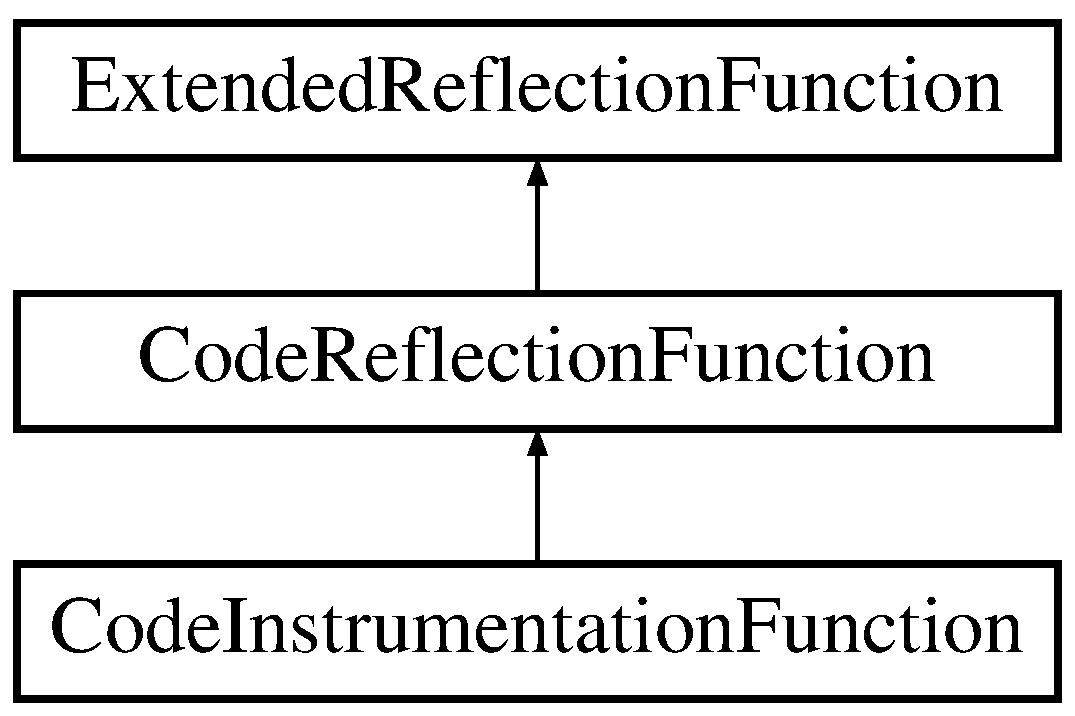
\includegraphics[height=3cm]{class_code_instrumentation_function}
\end{center}
\end{figure}
\subsection*{Protected Member Functions}
\begin{CompactItemize}
\item 
\hyperlink{class_code_instrumentation_function_3d95491ac661050b8e8ecedfaf3c8359}{createExtendedReflectionParameter} (ReflectionParameter \$objReflectionParameter)
\end{CompactItemize}


\subsection{Member Function Documentation}
\hypertarget{class_code_instrumentation_function_3d95491ac661050b8e8ecedfaf3c8359}{
\index{CodeInstrumentationFunction@{CodeInstrumentationFunction}!createExtendedReflectionParameter@{createExtendedReflectionParameter}}
\index{createExtendedReflectionParameter@{createExtendedReflectionParameter}!CodeInstrumentationFunction@{CodeInstrumentationFunction}}
\subsubsection[{createExtendedReflectionParameter}]{\setlength{\rightskip}{0pt plus 5cm}CodeInstrumentationFunction::createExtendedReflectionParameter (ReflectionParameter \$ {\em objReflectionParameter})\hspace{0.3cm}{\tt  \mbox{[}protected\mbox{]}}}}
\label{class_code_instrumentation_function_3d95491ac661050b8e8ecedfaf3c8359}


This method is necessary to make the callers of the parameters of the function bring CodeInstrumentationParameters

\begin{Desc}
\item[See also:]\hyperlink{class_extended_reflection_function_de07ccd452e54a7c8878fc20d215831e}{ExtendedReflectionFunction::createExtendedReflectionParameter} \end{Desc}
\begin{Desc}
\item[Parameters:]
\begin{description}
\item[{\em ReflectionParameter}]\$objReflectionParameter \end{description}
\end{Desc}
\begin{Desc}
\item[Returns:]\hyperlink{class_code_instrumentation_parameter}{CodeInstrumentationParameter} \end{Desc}


Reimplemented from \hyperlink{class_code_reflection_function_7ce14d3f6e8579332f226d85fb439b80}{CodeReflectionFunction}.

The documentation for this class was generated from the following file:\begin{CompactItemize}
\item 
components/codeInstrumentation/\hyperlink{_code_instrumentation_function_8class_8php}{CodeInstrumentationFunction.class.php}\end{CompactItemize}

\hypertarget{class_code_instrumentation_method}{
\section{CodeInstrumentationMethod Class Reference}
\label{class_code_instrumentation_method}\index{CodeInstrumentationMethod@{CodeInstrumentationMethod}}
}
Inheritance diagram for CodeInstrumentationMethod::\begin{figure}[H]
\begin{center}
\leavevmode
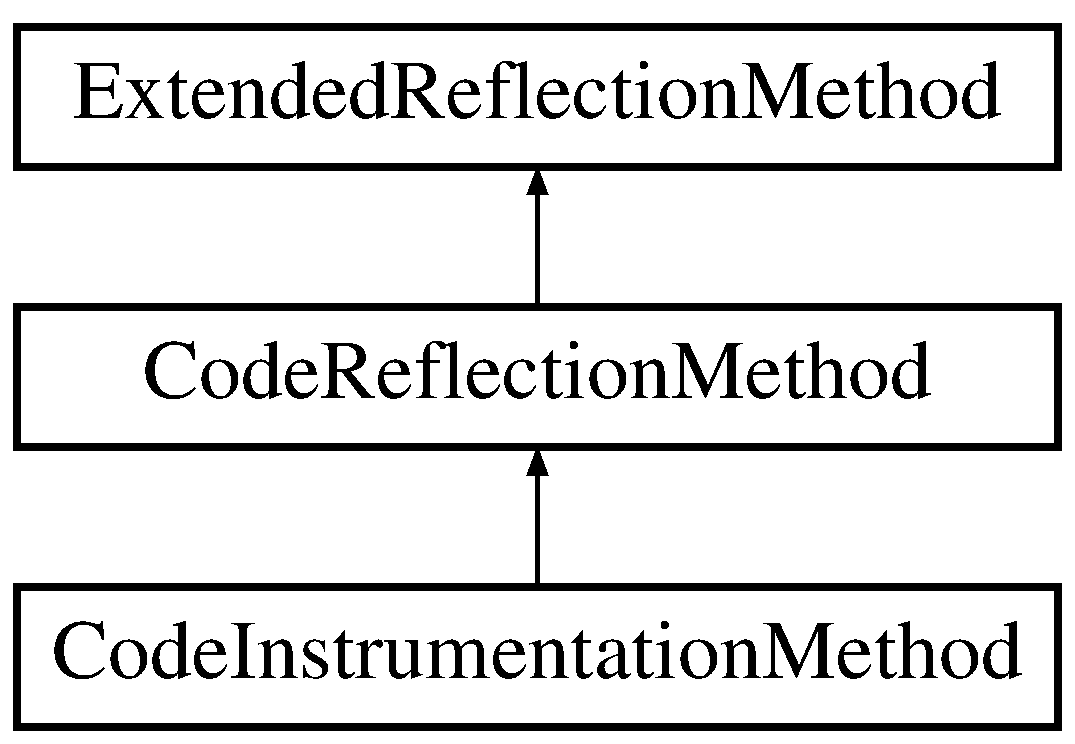
\includegraphics[height=3cm]{class_code_instrumentation_method}
\end{center}
\end{figure}
\subsection*{Public Member Functions}
\begin{CompactItemize}
\item 
\hyperlink{class_code_instrumentation_method_6e2855870a7381176413aa24a2fbfd43}{getNewName} ()
\item 
\hyperlink{class_code_instrumentation_method_7f82d49e30da995729069ae9190555da}{getCallCodeInstrFunctionName} ()
\item 
\hyperlink{class_code_instrumentation_method_b5e24da53b4a0d0848b18c1e832f47ff}{getCode} ()
\item 
\hyperlink{class_code_instrumentation_method_3d517292204047acfc6bb54cc09a38e3}{createMethodHeaderCode} ()
\end{CompactItemize}
\subsection*{Public Attributes}
\begin{CompactItemize}
\item 
const \hyperlink{class_code_instrumentation_method_459af7451a2f181e2e91e444c5a72d04}{PREFIX\_\-METHOD} = \char`\"{}\_\-\_\-\_\-\char`\"{}
\end{CompactItemize}
\subsection*{Protected Member Functions}
\begin{CompactItemize}
\item 
\hyperlink{class_code_instrumentation_method_5df850508e727984f62860b6987991c0}{getCallCodeInstrFunctionCode} ()
\item 
\hyperlink{class_code_instrumentation_method_bd8673f90786848f90fb3c0940c604a6}{getCallCodeInstrFunctionHeaderCode} ()
\item 
\hyperlink{class_code_instrumentation_method_ed55cb9e7235755c7fdab2dc01eb4f47}{getCallCodeInstrFunctionContentCode} ()
\item 
\hyperlink{class_code_instrumentation_method_6b56ec198bc6a5b5a72076e4e7c19e29}{createExtendedReflectionClass} (ReflectionClass \$objOriginalReflectionClass)
\item 
\hyperlink{class_code_instrumentation_method_98ceb248f2b535a3a83ac2e7990e0c1f}{createExtendedReflectionParameter} (ReflectionParameter \$objReflectionParameter)
\item 
\hyperlink{class_code_instrumentation_method_e38c2891dc093dabb6b363a4de9ac495}{createMethodContentCode} ()
\end{CompactItemize}


\subsection{Detailed Description}
Class what in place of create the exactly code of some method, create a version of it what send a message to the code instrumentation receiver before and after each call.

\begin{Desc}
\item[Author:]Thiago Henrique Ramos da Mata $<$\href{mailto:thiago.henrique.mata@gmail.com}{\tt thiago.henrique.mata@gmail.com}$>$ \end{Desc}


\subsection{Member Function Documentation}
\hypertarget{class_code_instrumentation_method_6b56ec198bc6a5b5a72076e4e7c19e29}{
\index{CodeInstrumentationMethod@{CodeInstrumentationMethod}!createExtendedReflectionClass@{createExtendedReflectionClass}}
\index{createExtendedReflectionClass@{createExtendedReflectionClass}!CodeInstrumentationMethod@{CodeInstrumentationMethod}}
\subsubsection[{createExtendedReflectionClass}]{\setlength{\rightskip}{0pt plus 5cm}createExtendedReflectionClass (ReflectionClass \$ {\em objOriginalReflectionClass})\hspace{0.3cm}{\tt  \mbox{[}protected\mbox{]}}}}
\label{class_code_instrumentation_method_6b56ec198bc6a5b5a72076e4e7c19e29}


make the class calls return a code instrumentation class

\begin{Desc}
\item[See also:]\hyperlink{class_extended_reflection_method}{ExtendedReflectionMethod} \end{Desc}
\begin{Desc}
\item[Parameters:]
\begin{description}
\item[{\em ReflectionClass}]\$objOriginalReflectionClass \end{description}
\end{Desc}
\begin{Desc}
\item[Returns:]\hyperlink{class_code_instrumentation_class}{CodeInstrumentationClass} \end{Desc}


Reimplemented from \hyperlink{class_code_reflection_method_6b56ec198bc6a5b5a72076e4e7c19e29}{CodeReflectionMethod}.

\begin{Code}\begin{verbatim}212     {
213         return new CodeInstrumentationClass( $objOriginalReflectionClass->getName() );
214     }
\end{verbatim}
\end{Code}


\hypertarget{class_code_instrumentation_method_98ceb248f2b535a3a83ac2e7990e0c1f}{
\index{CodeInstrumentationMethod@{CodeInstrumentationMethod}!createExtendedReflectionParameter@{createExtendedReflectionParameter}}
\index{createExtendedReflectionParameter@{createExtendedReflectionParameter}!CodeInstrumentationMethod@{CodeInstrumentationMethod}}
\subsubsection[{createExtendedReflectionParameter}]{\setlength{\rightskip}{0pt plus 5cm}createExtendedReflectionParameter (ReflectionParameter \$ {\em objReflectionParameter})\hspace{0.3cm}{\tt  \mbox{[}protected\mbox{]}}}}
\label{class_code_instrumentation_method_98ceb248f2b535a3a83ac2e7990e0c1f}


make the parameters calls return a Code Instrumentation Parameter

\begin{Desc}
\item[See also:]\hyperlink{class_extended_reflection_method_98ceb248f2b535a3a83ac2e7990e0c1f}{ExtendedReflectionMethod::createExtendedReflectionParameter} \end{Desc}
\begin{Desc}
\item[Parameters:]
\begin{description}
\item[{\em ReflectionParameter}]\$objReflectionParameter \end{description}
\end{Desc}
\begin{Desc}
\item[Returns:]\hyperlink{class_code_instrumentation_parameter}{CodeInstrumentationParameter} \end{Desc}


Reimplemented from \hyperlink{class_code_reflection_method_98ceb248f2b535a3a83ac2e7990e0c1f}{CodeReflectionMethod}.

\begin{Code}\begin{verbatim}224     {
225         return new CodeInstrumentationParameter( Array( $this->getDeclaringClass()->getName() , $this->getName() ) , $objReflectionParameter->getName() );
226     }
\end{verbatim}
\end{Code}


\hypertarget{class_code_instrumentation_method_e38c2891dc093dabb6b363a4de9ac495}{
\index{CodeInstrumentationMethod@{CodeInstrumentationMethod}!createMethodContentCode@{createMethodContentCode}}
\index{createMethodContentCode@{createMethodContentCode}!CodeInstrumentationMethod@{CodeInstrumentationMethod}}
\subsubsection[{createMethodContentCode}]{\setlength{\rightskip}{0pt plus 5cm}createMethodContentCode ()\hspace{0.3cm}{\tt  \mbox{[}protected\mbox{]}}}}
\label{class_code_instrumentation_method_e38c2891dc093dabb6b363a4de9ac495}


Create the code instrumentation method content code

\begin{Desc}
\item[Returns:]string \end{Desc}


Reimplemented from \hyperlink{class_code_reflection_method_e38c2891dc093dabb6b363a4de9ac495}{CodeReflectionMethod}.

\begin{Code}\begin{verbatim}234     {
235         $strCode = "";
236 
237         $objCodeInstrFile = CodeReflectionFile::getCodeInstrFileName( $this->getFileName() );
238         $strCode .= $objCodeInstrFile->getFileBit( $this->getStartLine() , $this->getEndLine() );
239         $strCode = trim( $strCode );
240 
241         if( strlen( $strCode ) == 0 )
242         {
243             return $strCode;
244         }
245         
246         // remove the { }
247         if( $strCode[0] == "{" )
248         {
249             $strCode = substr( $strCode , 1 );
250         }
251 
252         $intLast = strlen( $strCode ) - 1;
253 
254         if( $strCode[$intLast] == "}" )
255         {
256             $strCode = substr( $strCode , 0     , -1);
257         }
258         return $strCode;
259     }
\end{verbatim}
\end{Code}


\hypertarget{class_code_instrumentation_method_3d517292204047acfc6bb54cc09a38e3}{
\index{CodeInstrumentationMethod@{CodeInstrumentationMethod}!createMethodHeaderCode@{createMethodHeaderCode}}
\index{createMethodHeaderCode@{createMethodHeaderCode}!CodeInstrumentationMethod@{CodeInstrumentationMethod}}
\subsubsection[{createMethodHeaderCode}]{\setlength{\rightskip}{0pt plus 5cm}createMethodHeaderCode ()}}
\label{class_code_instrumentation_method_3d517292204047acfc6bb54cc09a38e3}


Get the method header of the code instrumentation method

\begin{Desc}
\item[Returns:]string \end{Desc}


Reimplemented from \hyperlink{class_code_reflection_method_3d517292204047acfc6bb54cc09a38e3}{CodeReflectionMethod}.

\begin{Code}\begin{verbatim}195     {
196         $strCode = $this->getDocComment();
197         $strCode .= $this->createModifiersCode();
198         $strCode .= " function ";
199         $strCode .= $this->getNewName();
200         $strCode .= $this->createParametersCode();
201         return CorujaStringManipulation::retab( $strCode , 1 );
202     }
\end{verbatim}
\end{Code}


\hypertarget{class_code_instrumentation_method_5df850508e727984f62860b6987991c0}{
\index{CodeInstrumentationMethod@{CodeInstrumentationMethod}!getCallCodeInstrFunctionCode@{getCallCodeInstrFunctionCode}}
\index{getCallCodeInstrFunctionCode@{getCallCodeInstrFunctionCode}!CodeInstrumentationMethod@{CodeInstrumentationMethod}}
\subsubsection[{getCallCodeInstrFunctionCode}]{\setlength{\rightskip}{0pt plus 5cm}getCallCodeInstrFunctionCode ()\hspace{0.3cm}{\tt  \mbox{[}protected\mbox{]}}}}
\label{class_code_instrumentation_method_5df850508e727984f62860b6987991c0}


Returns the code instrumentation method content what will be append into the class

\begin{Desc}
\item[Returns:]string \end{Desc}


\begin{Code}\begin{verbatim}48     {
49         $strCode = "";
50         $strCode .= $this->getCallCodeInstrFunctionHeaderCode();
51         $strCode .= "{" . "\n";
52         $strCode .= $this->getCallCodeInstrFunctionContentCode();
53         $strCode .= "}" . "\n";
54         return $strCode;
55     }
\end{verbatim}
\end{Code}


\hypertarget{class_code_instrumentation_method_ed55cb9e7235755c7fdab2dc01eb4f47}{
\index{CodeInstrumentationMethod@{CodeInstrumentationMethod}!getCallCodeInstrFunctionContentCode@{getCallCodeInstrFunctionContentCode}}
\index{getCallCodeInstrFunctionContentCode@{getCallCodeInstrFunctionContentCode}!CodeInstrumentationMethod@{CodeInstrumentationMethod}}
\subsubsection[{getCallCodeInstrFunctionContentCode}]{\setlength{\rightskip}{0pt plus 5cm}getCallCodeInstrFunctionContentCode ()\hspace{0.3cm}{\tt  \mbox{[}protected\mbox{]}}}}
\label{class_code_instrumentation_method_ed55cb9e7235755c7fdab2dc01eb4f47}


Get the code instrumentation content of the method what will be append into the class

1. create the method header 2. if the method is a static one 2.1 log the enter method into the code instrumentation receiver as a static call 2.2 run method 2.3 log the leave method into the code instrumentation receiver as a static call 3. else - if the method is not a static one 3.1 log the enter method into the code instrumentation receiver sending the object id 3.2 if the method is the magic method \_\-\_\-call 3.2.1 when some undefined method be called log the call and call the original \_\-\_\-call 3.3 else - if the method is not the magic method \_\-\_\-call 3.3.1 save the call into the code instrumentation receiver and call the original method 3.4 log the leave method into the code instrumentation receiver sending the object id

\begin{Desc}
\item[Returns:]string \end{Desc}


\begin{Code}\begin{verbatim}92     {
93                 // 1. create the method header //
94         $strCode = "";
95         $strCode .=     '       $strMethod = "' . $this->getNewName() . '";                                                                             ' . "\n";
96         $strCode .=     '       $arrArguments = func_get_args();                                                                                                ' . "\n";
97         $strCode .=     '       // prepare caller //                                                                                                                    ' . "\n";
98         
99         // 2. if the method is a static one //
100         if( $this->isStatic() )
101         {
102                      // 2.1 log the enter method into the code instrumentation receiver as a static call
103             $strCode .= '       $arrCaller = Array( __CLASS__ , $strMethod ) ;                                                          ' . "\n";
104             $strCode .= '       // log the enter into the real method //                                                                                ' . "\n";
105             $strCode .= '       CodeInstrumentationReceiver::getInstance()->onEnterMethod( "static" , __CLASS__ , __METHOD__ , $arrArguments );' . "\n";
106 
107             // 2.2 run method
108             $strCode .= '       // execute the real method                                                                                                              ' . "\n";
109             $strCode .= '       $mixReturn = call_user_func_array( $arrCaller, $arrArguments );                                 ' . "\n";
110 
111                     // 2.3 log the leave method into the code instrumentation receiver as a static call
112             $strCode .= '       // log the exit of the real method //                                                                                   ' . "\n";
113             $strCode .= '       CodeInstrumentationReceiver::getInstance()->onLeaveMethod( "static" , __CLASS__ , __METHOD__ , $mixReturn    );' . "\n";
114             $strCode .= '       // return the result of the method into the object  //                                                  ' . "\n";
115             $strCode .= '       return $mixReturn;                                                                                                                              ' . "\n";
116         }
117         // 3. else - if the method is not a static one //
118         else
119         {
120                 // 3.1 log the enter method into the code instrumentation receiver sending the object id //
121             $strCode .= '       $arrCaller = Array( $this , $strMethod ) ;                                      ' . "\n";
122             $strCode .= '       // log the enter into the real method //                                        ' . "\n";
123             $strCode .= '       CodeInstrumentationReceiver::getInstance()->onEnterMethod( spl_object_hash($this) , __CLASS__ , __METHOD__ , $arrArguments );' . "\n";
124             $strCode .= '       // execute the real method                                                      ' . "\n";
125             
126             // 3.2 if the method is the magic method __call //
127             if( $this->getName() == "__call" )
128             {
129                 // 3.2.1 when some undefined method be called log the call and call the original __call //
130                 $strCode .=     '       // if the method exists                                                                                                         ' . "\n";
131                 $strCode .=     '       if( method_exists( $this , $strMethod ) )                                                                               ' . "\n";
132                 $strCode .=     '       {                                                                               ' . "\n";
133                 $strCode .=     '           // call the real method                                                     ' . "\n";
134                 $strCode .=     '       $mixReturn = call_user_func_array( $arrCaller, $arrArguments );                         ' . "\n";
135                 $strCode .=     '       }                                                                               ' . "\n";
136                 $strCode .=     '       else                                                                            ' . "\n";
137                 $strCode .=     '       {                                                                               ' . "\n";
138                 $strCode .=     '           // exists in the original class a __call method //                          ' . "\n";
139                 $strCode .=     '           if( method_exists( $this , "' . self::PREFIX_METHOD . '__call" ) )                                   ' . "\n";
140                 $strCode .=     '           {                                                                           ' . "\n";
141                 $strCode .=     '               // call it //                                                           ' . "\n";
142                 $strCode .=     '               $mixReturn = $this->' . self::PREFIX_METHOD . '__call( $strMethod , $arrArguments );                          ' . "\n";
143                 $strCode .=     '           }                                                                           ' . "\n";
144                 $strCode .=     '           else                                                                           ' . "\n";
145                 $strCode .=     '           {                                                                           ' . "\n";
146                 $strCode .=     '           throw new CodeToDiagramException( "Unable to find the method $strMethod "); ' . "\n";
147                 $strCode .=     '           }                                                                           ' . "\n";
148                 $strCode .=     '       }                                                                               ' . "\n";
149             }
150             // 3.3 else - if the method is not the magic method __call //
151             else
152             {
153                 //  3.3.1 save the call into the code instrumentation receiver and call the original method //
154                 $strCode .=     '       // if the method exists                                                                                                         ' . "\n";
155                 $strCode .=     '       if( method_exists( $this , $strMethod ) )                                                                               ' . "\n";
156                 $strCode .=     '       {                                                                               ' . "\n";
157                 $strCode .=     '           // call the real method                                                     ' . "\n";
158                 $strCode .=     '       $mixReturn = call_user_func_array( $arrCaller, $arrArguments );                         ' . "\n";
159                 $strCode .=     '       }                                                                               ' . "\n";
160                 $strCode .=     '       else                                                                            ' . "\n";
161                 $strCode .=     '       {                                                                               ' . "\n";
162                 $strCode .=     '       throw new CodeToDiagramException( "Unable to find the method $strMethod "); ' . "\n";
163                 $strCode .=     '       }                                                                               ' . "\n";
164             }
165             // 3.4 log the leave method into the code instrumentation receiver sending the object id
166             $strCode .= '       // log the exit of the real method //                                                                                   ' . "\n";
167             $strCode .= '       CodeInstrumentationReceiver::getInstance()->onLeaveMethod( spl_object_hash($this) , __CLASS__ , __METHOD__ , $mixReturn    );' . "\n";
168             $strCode .= '       // return the result of the method into the object  //                                                  ' . "\n";
169             $strCode .= '       return $mixReturn;                                                                                                                              ' . "\n";
170         }
171 
172         return $strCode;
173     }
\end{verbatim}
\end{Code}


\hypertarget{class_code_instrumentation_method_bd8673f90786848f90fb3c0940c604a6}{
\index{CodeInstrumentationMethod@{CodeInstrumentationMethod}!getCallCodeInstrFunctionHeaderCode@{getCallCodeInstrFunctionHeaderCode}}
\index{getCallCodeInstrFunctionHeaderCode@{getCallCodeInstrFunctionHeaderCode}!CodeInstrumentationMethod@{CodeInstrumentationMethod}}
\subsubsection[{getCallCodeInstrFunctionHeaderCode}]{\setlength{\rightskip}{0pt plus 5cm}getCallCodeInstrFunctionHeaderCode ()\hspace{0.3cm}{\tt  \mbox{[}protected\mbox{]}}}}
\label{class_code_instrumentation_method_bd8673f90786848f90fb3c0940c604a6}


Get the code instrumentation header of the method what will be append into the class

\begin{Desc}
\item[Returns:]string \end{Desc}


\begin{Code}\begin{verbatim}64     {
65         $strCode = CorujaStringManipulation::retab( $this->getDocComment() , 1 );
66         $strCode .= $this->createModifiersCode();
67         $strCode .= " function " . $this->getCallCodeInstrFunctionName();
68         $strCode .= $this->createParametersCode();
69         return $strCode;
70     }
\end{verbatim}
\end{Code}


\hypertarget{class_code_instrumentation_method_7f82d49e30da995729069ae9190555da}{
\index{CodeInstrumentationMethod@{CodeInstrumentationMethod}!getCallCodeInstrFunctionName@{getCallCodeInstrFunctionName}}
\index{getCallCodeInstrFunctionName@{getCallCodeInstrFunctionName}!CodeInstrumentationMethod@{CodeInstrumentationMethod}}
\subsubsection[{getCallCodeInstrFunctionName}]{\setlength{\rightskip}{0pt plus 5cm}getCallCodeInstrFunctionName ()}}
\label{class_code_instrumentation_method_7f82d49e30da995729069ae9190555da}


Returns de name of the code instrumentation method name what will be append into the class

\begin{Desc}
\item[Returns:]string \end{Desc}


\begin{Code}\begin{verbatim}38     {
39         return $this->getName();
40     }
\end{verbatim}
\end{Code}


\hypertarget{class_code_instrumentation_method_b5e24da53b4a0d0848b18c1e832f47ff}{
\index{CodeInstrumentationMethod@{CodeInstrumentationMethod}!getCode@{getCode}}
\index{getCode@{getCode}!CodeInstrumentationMethod@{CodeInstrumentationMethod}}
\subsubsection[{getCode}]{\setlength{\rightskip}{0pt plus 5cm}getCode ()}}
\label{class_code_instrumentation_method_b5e24da53b4a0d0848b18c1e832f47ff}


Get the code of the code instrumentation method

\begin{Desc}
\item[Returns:]string \end{Desc}


Reimplemented from \hyperlink{class_code_reflection_method_b5e24da53b4a0d0848b18c1e832f47ff}{CodeReflectionMethod}.

\begin{Code}\begin{verbatim}181     {
182         $strCode = "";
183         $strCode .= $this->getCallCodeInstrFunctionCode();
184         $strCode .= parent::getCode();
185         return $strCode;
186 
187     }
\end{verbatim}
\end{Code}


\hypertarget{class_code_instrumentation_method_6e2855870a7381176413aa24a2fbfd43}{
\index{CodeInstrumentationMethod@{CodeInstrumentationMethod}!getNewName@{getNewName}}
\index{getNewName@{getNewName}!CodeInstrumentationMethod@{CodeInstrumentationMethod}}
\subsubsection[{getNewName}]{\setlength{\rightskip}{0pt plus 5cm}getNewName ()}}
\label{class_code_instrumentation_method_6e2855870a7381176413aa24a2fbfd43}


Returns the new name of the original method. ' \begin{Desc}
\item[Returns:]string \end{Desc}


\begin{Code}\begin{verbatim}28     {
29         return self::PREFIX_METHOD . $this->getName();
30     }
\end{verbatim}
\end{Code}




\subsection{Member Data Documentation}
\hypertarget{class_code_instrumentation_method_459af7451a2f181e2e91e444c5a72d04}{
\index{CodeInstrumentationMethod@{CodeInstrumentationMethod}!PREFIX\_\-METHOD@{PREFIX\_\-METHOD}}
\index{PREFIX\_\-METHOD@{PREFIX\_\-METHOD}!CodeInstrumentationMethod@{CodeInstrumentationMethod}}
\subsubsection[{PREFIX\_\-METHOD}]{\setlength{\rightskip}{0pt plus 5cm}const {\bf PREFIX\_\-METHOD} = \char`\"{}\_\-\_\-\_\-\char`\"{}}}
\label{class_code_instrumentation_method_459af7451a2f181e2e91e444c5a72d04}


The original method should be renamed. This is the new prefix what will be append into it's name. 

The documentation for this class was generated from the following file:\begin{CompactItemize}
\item 
components/codeInstrumentation/\hyperlink{_code_instrumentation_method_8class_8php}{CodeInstrumentationMethod.class.php}\end{CompactItemize}

\hypertarget{class_code_instrumentation_parameter}{
\section{CodeInstrumentationParameter Class Reference}
\label{class_code_instrumentation_parameter}\index{CodeInstrumentationParameter@{CodeInstrumentationParameter}}
}
Inheritance diagram for CodeInstrumentationParameter::\begin{figure}[H]
\begin{center}
\leavevmode
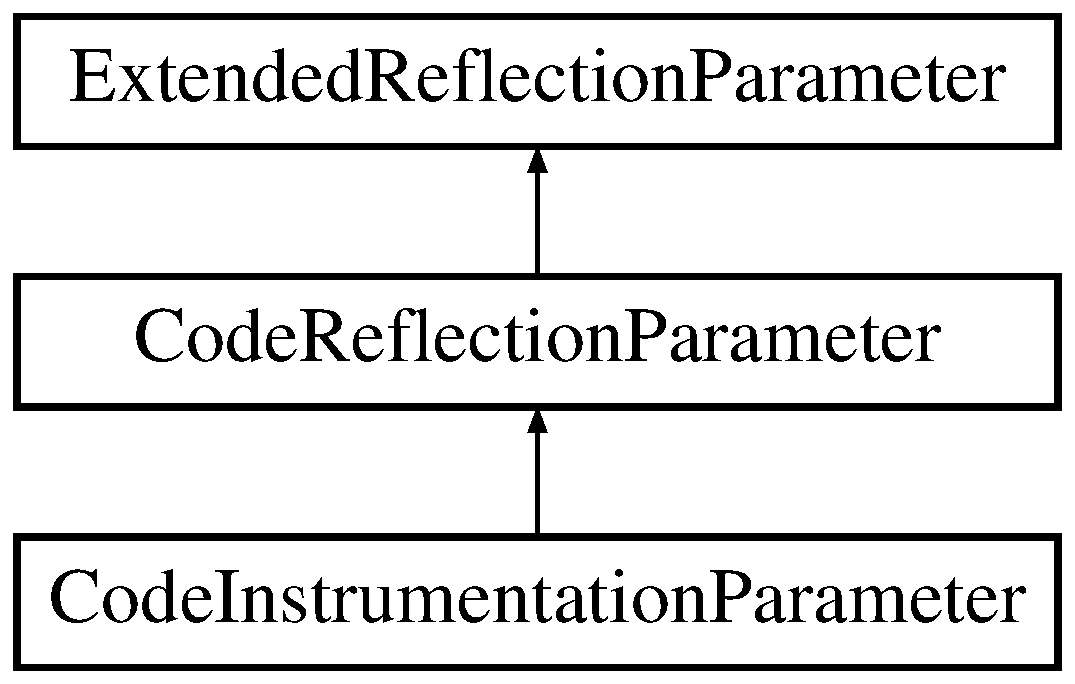
\includegraphics[height=3cm]{class_code_instrumentation_parameter}
\end{center}
\end{figure}
\subsection*{Protected Member Functions}
\begin{CompactItemize}
\item 
\hyperlink{class_code_instrumentation_parameter_4190025f9ec55f58f10b36084a8851fd}{createExtendedReflectionClass} (ReflectionClass \$objOriginalReflectionClass)
\item 
\hyperlink{class_code_instrumentation_parameter_e0c68e69aa93979e2e1fa3057bd39d5a}{createExtendedReflectionMethod} (ReflectionMethod \$objOriginalReflectionMethod)
\item 
\hyperlink{class_code_instrumentation_parameter_e9723a389b48bdb31fc49f784692aecf}{createExtendedReflectionFunction} (ReflectionFunction \$objOriginalReflectionFunction)
\end{CompactItemize}


\subsection{Member Function Documentation}
\hypertarget{class_code_instrumentation_parameter_4190025f9ec55f58f10b36084a8851fd}{
\index{CodeInstrumentationParameter@{CodeInstrumentationParameter}!createExtendedReflectionClass@{createExtendedReflectionClass}}
\index{createExtendedReflectionClass@{createExtendedReflectionClass}!CodeInstrumentationParameter@{CodeInstrumentationParameter}}
\subsubsection[{createExtendedReflectionClass}]{\setlength{\rightskip}{0pt plus 5cm}CodeInstrumentationParameter::createExtendedReflectionClass (ReflectionClass \$ {\em objOriginalReflectionClass})\hspace{0.3cm}{\tt  \mbox{[}protected\mbox{]}}}}
\label{class_code_instrumentation_parameter_4190025f9ec55f58f10b36084a8851fd}


Replace the original reflection class by the Code Instrumentation version of it

\begin{Desc}
\item[Parameters:]
\begin{description}
\item[{\em ReflectionClass}]\$objOriginalReflectionClass \end{description}
\end{Desc}
\begin{Desc}
\item[Returns:]CodeInstrumentationClass \end{Desc}


Reimplemented from \hyperlink{class_code_reflection_parameter_a2b9b21f9711afbf11791dd64dcbdd0a}{CodeReflectionParameter}.\hypertarget{class_code_instrumentation_parameter_e9723a389b48bdb31fc49f784692aecf}{
\index{CodeInstrumentationParameter@{CodeInstrumentationParameter}!createExtendedReflectionFunction@{createExtendedReflectionFunction}}
\index{createExtendedReflectionFunction@{createExtendedReflectionFunction}!CodeInstrumentationParameter@{CodeInstrumentationParameter}}
\subsubsection[{createExtendedReflectionFunction}]{\setlength{\rightskip}{0pt plus 5cm}CodeInstrumentationParameter::createExtendedReflectionFunction (ReflectionFunction \$ {\em objOriginalReflectionFunction})\hspace{0.3cm}{\tt  \mbox{[}protected\mbox{]}}}}
\label{class_code_instrumentation_parameter_e9723a389b48bdb31fc49f784692aecf}


Replace the origianl reflection function of the parameters by the code instrumentation version of it

\begin{Desc}
\item[Parameters:]
\begin{description}
\item[{\em ReflectionFunction}]\$objOriginalReflectionFunction \end{description}
\end{Desc}
\begin{Desc}
\item[Returns:]\hyperlink{class_code_instrumentation_function}{CodeInstrumentationFunction} \end{Desc}


Reimplemented from \hyperlink{class_code_reflection_parameter_5e6e7a1f49ff1f404342a2b2d4a15aa3}{CodeReflectionParameter}.\hypertarget{class_code_instrumentation_parameter_e0c68e69aa93979e2e1fa3057bd39d5a}{
\index{CodeInstrumentationParameter@{CodeInstrumentationParameter}!createExtendedReflectionMethod@{createExtendedReflectionMethod}}
\index{createExtendedReflectionMethod@{createExtendedReflectionMethod}!CodeInstrumentationParameter@{CodeInstrumentationParameter}}
\subsubsection[{createExtendedReflectionMethod}]{\setlength{\rightskip}{0pt plus 5cm}CodeInstrumentationParameter::createExtendedReflectionMethod (ReflectionMethod \$ {\em objOriginalReflectionMethod})\hspace{0.3cm}{\tt  \mbox{[}protected\mbox{]}}}}
\label{class_code_instrumentation_parameter_e0c68e69aa93979e2e1fa3057bd39d5a}


Replace the original reflection method by the Code Instrumentation version of it

\begin{Desc}
\item[Parameters:]
\begin{description}
\item[{\em ReflectionMethod}]\$objOriginalReflectionMethod \end{description}
\end{Desc}
\begin{Desc}
\item[Returns:]\hyperlink{class_code_instrumentation_method}{CodeInstrumentationMethod} \end{Desc}


Reimplemented from \hyperlink{class_code_reflection_parameter_04d7dbd71bc943f3e267869a79bec648}{CodeReflectionParameter}.

The documentation for this class was generated from the following file:\begin{CompactItemize}
\item 
components/codeInstrumentation/\hyperlink{_code_instrumentation_parameter_8class_8php}{CodeInstrumentationParameter.class.php}\end{CompactItemize}

\hypertarget{class_code_instrumentation_property}{
\section{CodeInstrumentationProperty Class Reference}
\label{class_code_instrumentation_property}\index{CodeInstrumentationProperty@{CodeInstrumentationProperty}}
}
Inheritance diagram for CodeInstrumentationProperty::\begin{figure}[H]
\begin{center}
\leavevmode
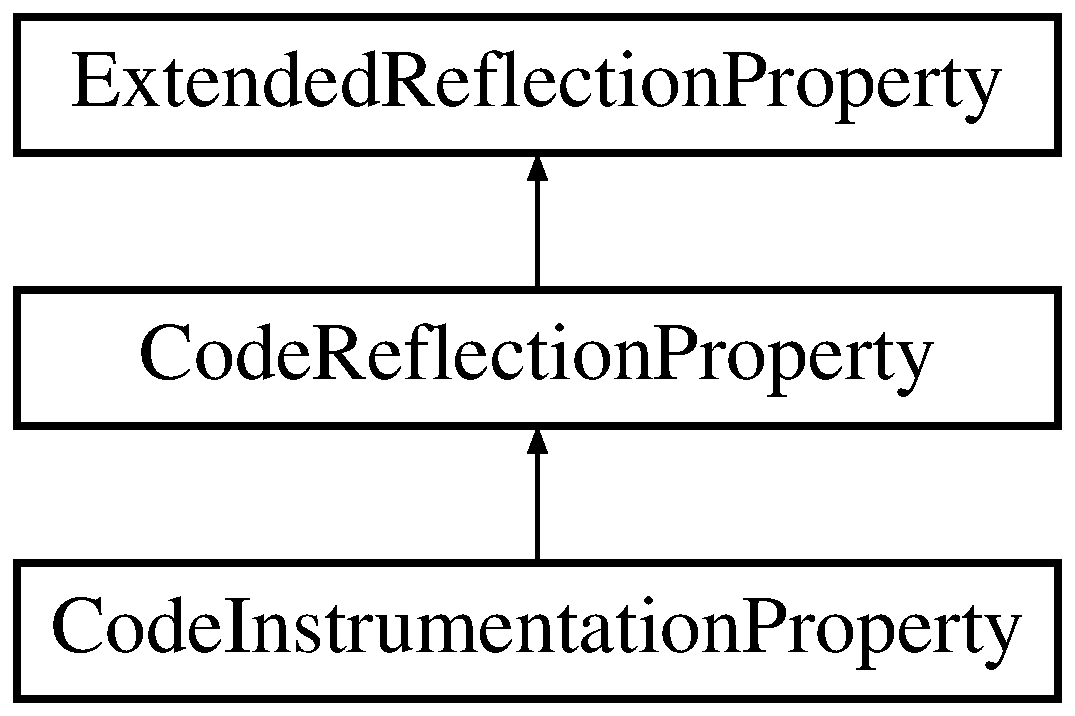
\includegraphics[height=3cm]{class_code_instrumentation_property}
\end{center}
\end{figure}
\subsection*{Protected Member Functions}
\begin{CompactItemize}
\item 
\hyperlink{class_code_instrumentation_property_6b56ec198bc6a5b5a72076e4e7c19e29}{createExtendedReflectionClass} (ReflectionClass \$objOriginalReflectionClass)
\end{CompactItemize}


\subsection{Detailed Description}
class necessary to make the code instrumentation process possible

the propery has not big changes of the code reflection property but it is necessary to extend it to create the reflections links possibles keeping the code instrumentation context.

\begin{Desc}
\item[Author:]Thiago Henrique Ramos da Mata $<$\href{mailto:thiago.henrique.mata@gmail.com}{\tt thiago.henrique.mata@gmail.com}$>$ \end{Desc}


\subsection{Member Function Documentation}
\hypertarget{class_code_instrumentation_property_6b56ec198bc6a5b5a72076e4e7c19e29}{
\index{CodeInstrumentationProperty@{CodeInstrumentationProperty}!createExtendedReflectionClass@{createExtendedReflectionClass}}
\index{createExtendedReflectionClass@{createExtendedReflectionClass}!CodeInstrumentationProperty@{CodeInstrumentationProperty}}
\subsubsection[{createExtendedReflectionClass}]{\setlength{\rightskip}{0pt plus 5cm}createExtendedReflectionClass (ReflectionClass \$ {\em objOriginalReflectionClass})\hspace{0.3cm}{\tt  \mbox{[}protected\mbox{]}}}}
\label{class_code_instrumentation_property_6b56ec198bc6a5b5a72076e4e7c19e29}


Make the calls to the reflection class of the property return a Code Instrumentation class

\begin{Desc}
\item[See also:]CodeReflectionProperty::createExtendedReflectionClass( ReflectionClass ) 

CodeReflectionProperty::createExtendedReflectionClass( ReflectionClass ) \end{Desc}


Reimplemented from \hyperlink{class_code_reflection_property_6b56ec198bc6a5b5a72076e4e7c19e29}{CodeReflectionProperty}.

\begin{Code}\begin{verbatim}27     {
28         return new CodeInstrumentationClass( $objOriginalReflectionClass->getName() );
29     }
\end{verbatim}
\end{Code}




The documentation for this class was generated from the following file:\begin{CompactItemize}
\item 
components/codeInstrumentation/\hyperlink{_code_instrumentation_property_8class_8php}{CodeInstrumentationProperty.class.php}\end{CompactItemize}

\hypertarget{class_code_instrumentation_receiver}{
\section{CodeInstrumentationReceiver Class Reference}
\label{class_code_instrumentation_receiver}\index{CodeInstrumentationReceiver@{CodeInstrumentationReceiver}}
}
\subsection*{Public Member Functions}
\begin{CompactItemize}
\item 
\hyperlink{class_code_instrumentation_receiver_6d6ba9a97475d3f300ec905ef3fc6d7a}{setIgnoreNullReturns} (\$booIgnoreNullReturns)
\item 
\hyperlink{class_code_instrumentation_receiver_659ec50b656faab0ff518cce0cbe1a43}{getIgnoreNullReturns} ()
\item 
\hyperlink{class_code_instrumentation_receiver_d9b3988e912a93b15037235ee4150e5a}{setIgnoreRecursiveCalls} (\$booIgnoreRecursiveCalls)
\item 
\hyperlink{class_code_instrumentation_receiver_f5d40f3016b4d1b289a089b24eebbbe5}{getIgnoreRecursiveCalls} ()
\item 
\hyperlink{class_code_instrumentation_receiver_187013c79a78480d90269bd6e66c6772}{setCallerPath} (\$strCallerPath)
\item 
\hyperlink{class_code_instrumentation_receiver_8e5e85fb7a58ef069788033b05ba0004}{getCallerPath} ()
\item 
\hyperlink{class_code_instrumentation_receiver_5a1555be1d4979c83dbdbacdfc31c679}{setPublicPath} (\$strPublicPath)
\item 
\hyperlink{class_code_instrumentation_receiver_7eceb6a70b026359b2428df86b7e1d5d}{getPublicPath} ()
\item 
\hyperlink{class_code_instrumentation_receiver_118198dd8eaf3a12e3bbc407a92a3376}{\_\-\_\-construct} ()
\item 
\hyperlink{class_code_instrumentation_receiver_f103bccb49a8e11c8da7d4a12bee14cc}{renameMethod} (\$strMethod)
\item 
\hyperlink{class_code_instrumentation_receiver_51bfc5d088d4cf97f850a64cc9b76944}{onEnterMethod} (\$uid, \$strClassDefinition, \$strMethod, \$arrArguments)
\item 
\hyperlink{class_code_instrumentation_receiver_dbe8202a28014f81a7c18f59f557fadc}{onLeaveMethod} (\$uid, \$strClassDefinition, \$strMethod, \$mixReturn)
\item 
\hyperlink{class_code_instrumentation_receiver_addf964fe411ef0c9d4caa4745d22a31}{getXmlSequence} ()
\item 
\hyperlink{class_code_instrumentation_receiver_7f475c5ce6f32c9ab0aac748646deaa8}{restart} ()
\end{CompactItemize}
\subsection*{Static Public Member Functions}
\begin{CompactItemize}
\item 
static \hyperlink{class_code_instrumentation_receiver_7a8b6e3e36c2e6d9fb87f11c8f0aae9b}{getInstance} ()
\end{CompactItemize}
\subsection*{Static Public Attributes}
\begin{CompactItemize}
\item 
static \hyperlink{class_code_instrumentation_receiver_58ceb69302146200d34d39e5f8054301}{\$objCodeInstrumentationReceiver}
\end{CompactItemize}
\subsection*{Protected Attributes}
\begin{CompactItemize}
\item 
\hyperlink{class_code_instrumentation_receiver_9ebcf638caafb0ea92b785a30f8d5cd1}{\$booIgnoreNullReturns} = true
\item 
\hyperlink{class_code_instrumentation_receiver_208637de519d149d33197e681cccb395}{\$booIgnoreRecursiveCalls} = false
\item 
\hyperlink{class_code_instrumentation_receiver_9e8be5e4b9207833e7d3e92e25c5f797}{\$booMergeSameClassObjects} = false
\item 
\hyperlink{class_code_instrumentation_receiver_fb6ce3e590b5b38b793070943bca71f0}{\$arrStack} = array()
\item 
\hyperlink{class_code_instrumentation_receiver_5945968b33462c2a11548cf19ffa66ad}{\$arrActors} = array()
\item 
\hyperlink{class_code_instrumentation_receiver_3f358c2cfe75b8443ba3d0b908fbdd4c}{\$arrClasses} = array()
\item 
\hyperlink{class_code_instrumentation_receiver_231ad79a1ae080f3dda3388819d90247}{\$arrMessages} = array()
\item 
\hyperlink{class_code_instrumentation_receiver_7e81a184fa4092dd95506d434c2660ff}{\$objXmlSequence} = null
\end{CompactItemize}


\subsection{Constructor \& Destructor Documentation}
\hypertarget{class_code_instrumentation_receiver_118198dd8eaf3a12e3bbc407a92a3376}{
\index{CodeInstrumentationReceiver@{CodeInstrumentationReceiver}!\_\-\_\-construct@{\_\-\_\-construct}}
\index{\_\-\_\-construct@{\_\-\_\-construct}!CodeInstrumentationReceiver@{CodeInstrumentationReceiver}}
\subsubsection[{\_\-\_\-construct}]{\setlength{\rightskip}{0pt plus 5cm}CodeInstrumentationReceiver::\_\-\_\-construct ()}}
\label{class_code_instrumentation_receiver_118198dd8eaf3a12e3bbc407a92a3376}


prepare the code instrumentation receiver to start to receive the informations about the execution.

1. create the xml sequence object 2. create the user actor

\begin{Desc}
\item[Returns:]null \end{Desc}


\subsection{Member Function Documentation}
\hypertarget{class_code_instrumentation_receiver_8e5e85fb7a58ef069788033b05ba0004}{
\index{CodeInstrumentationReceiver@{CodeInstrumentationReceiver}!getCallerPath@{getCallerPath}}
\index{getCallerPath@{getCallerPath}!CodeInstrumentationReceiver@{CodeInstrumentationReceiver}}
\subsubsection[{getCallerPath}]{\setlength{\rightskip}{0pt plus 5cm}CodeInstrumentationReceiver::getCallerPath ()}}
\label{class_code_instrumentation_receiver_8e5e85fb7a58ef069788033b05ba0004}


Get the caller path of the xml sequence of the code instrumentation receiver

\begin{Desc}
\item[See also:]\hyperlink{class_xml_sequence_197ff62ed0c4d22324218206147f25e4}{XmlSequence::getCallerPath} \end{Desc}
\begin{Desc}
\item[Returns:]string \end{Desc}
\hypertarget{class_code_instrumentation_receiver_659ec50b656faab0ff518cce0cbe1a43}{
\index{CodeInstrumentationReceiver@{CodeInstrumentationReceiver}!getIgnoreNullReturns@{getIgnoreNullReturns}}
\index{getIgnoreNullReturns@{getIgnoreNullReturns}!CodeInstrumentationReceiver@{CodeInstrumentationReceiver}}
\subsubsection[{getIgnoreNullReturns}]{\setlength{\rightskip}{0pt plus 5cm}CodeInstrumentationReceiver::getIgnoreNullReturns ()}}
\label{class_code_instrumentation_receiver_659ec50b656faab0ff518cce0cbe1a43}


get the configuration paramenter if the code instrumentation should ignore the returns messages with null value returned.

\begin{Desc}
\item[See also:]CodeInstrumentationReceiver-$>$boolIgnoreNullReturns 

CodeInstrumentationReceiver::seIgnoreNullReturns( boolean ) \end{Desc}
\begin{Desc}
\item[Returns:]boolean {\tt true} if should ignore the null returns \end{Desc}
\hypertarget{class_code_instrumentation_receiver_f5d40f3016b4d1b289a089b24eebbbe5}{
\index{CodeInstrumentationReceiver@{CodeInstrumentationReceiver}!getIgnoreRecursiveCalls@{getIgnoreRecursiveCalls}}
\index{getIgnoreRecursiveCalls@{getIgnoreRecursiveCalls}!CodeInstrumentationReceiver@{CodeInstrumentationReceiver}}
\subsubsection[{getIgnoreRecursiveCalls}]{\setlength{\rightskip}{0pt plus 5cm}CodeInstrumentationReceiver::getIgnoreRecursiveCalls ()}}
\label{class_code_instrumentation_receiver_f5d40f3016b4d1b289a089b24eebbbe5}


get the configuration paramenter if the code instrumentation should ignore the recursive messages.

\begin{Desc}
\item[See also:]CodeInstrumentationReceiver-$>$booIgnoreRecursiveCalls 

CodeInstrumentationReceiver::setIgnoreRecursiveCalls( boolean ) \end{Desc}
\begin{Desc}
\item[Parameters:]
\begin{description}
\item[{\em \$booIgnoreNullReturns}]{\tt true} if should ignore the null returns \end{description}
\end{Desc}
\begin{Desc}
\item[Returns:]boolean {\tt true} if should ignore the recursive calls \end{Desc}
\hypertarget{class_code_instrumentation_receiver_7a8b6e3e36c2e6d9fb87f11c8f0aae9b}{
\index{CodeInstrumentationReceiver@{CodeInstrumentationReceiver}!getInstance@{getInstance}}
\index{getInstance@{getInstance}!CodeInstrumentationReceiver@{CodeInstrumentationReceiver}}
\subsubsection[{getInstance}]{\setlength{\rightskip}{0pt plus 5cm}static CodeInstrumentationReceiver::getInstance ()\hspace{0.3cm}{\tt  \mbox{[}static\mbox{]}}}}
\label{class_code_instrumentation_receiver_7a8b6e3e36c2e6d9fb87f11c8f0aae9b}


Get the code instrumentation receiver singleton

\begin{Desc}
\item[Returns:]\hyperlink{class_code_instrumentation_receiver}{CodeInstrumentationReceiver} \end{Desc}
\hypertarget{class_code_instrumentation_receiver_7eceb6a70b026359b2428df86b7e1d5d}{
\index{CodeInstrumentationReceiver@{CodeInstrumentationReceiver}!getPublicPath@{getPublicPath}}
\index{getPublicPath@{getPublicPath}!CodeInstrumentationReceiver@{CodeInstrumentationReceiver}}
\subsubsection[{getPublicPath}]{\setlength{\rightskip}{0pt plus 5cm}CodeInstrumentationReceiver::getPublicPath ()}}
\label{class_code_instrumentation_receiver_7eceb6a70b026359b2428df86b7e1d5d}


Get the \hyperlink{namespacepublic}{public} path of the xml sequence of the code instrumentation receiver

\begin{Desc}
\item[See also:]\hyperlink{class_xml_sequence_156bcaa4792dca6a381621d68052ba32}{XmlSequence::getPublicPath} \end{Desc}
\begin{Desc}
\item[Returns:]string \end{Desc}
\hypertarget{class_code_instrumentation_receiver_addf964fe411ef0c9d4caa4745d22a31}{
\index{CodeInstrumentationReceiver@{CodeInstrumentationReceiver}!getXmlSequence@{getXmlSequence}}
\index{getXmlSequence@{getXmlSequence}!CodeInstrumentationReceiver@{CodeInstrumentationReceiver}}
\subsubsection[{getXmlSequence}]{\setlength{\rightskip}{0pt plus 5cm}CodeInstrumentationReceiver::getXmlSequence ()}}
\label{class_code_instrumentation_receiver_addf964fe411ef0c9d4caa4745d22a31}


Return the Xml Sequence Object what the Code Instrumentation Receiver feeds

\begin{Desc}
\item[Returns:]\hyperlink{class_xml_sequence}{XmlSequence} \end{Desc}
\hypertarget{class_code_instrumentation_receiver_51bfc5d088d4cf97f850a64cc9b76944}{
\index{CodeInstrumentationReceiver@{CodeInstrumentationReceiver}!onEnterMethod@{onEnterMethod}}
\index{onEnterMethod@{onEnterMethod}!CodeInstrumentationReceiver@{CodeInstrumentationReceiver}}
\subsubsection[{onEnterMethod}]{\setlength{\rightskip}{0pt plus 5cm}CodeInstrumentationReceiver::onEnterMethod (\$ {\em uid}, \/  \$ {\em strClassDefinition}, \/  \$ {\em strMethod}, \/  \$ {\em arrArguments})}}
\label{class_code_instrumentation_receiver_51bfc5d088d4cf97f850a64cc9b76944}


Receive a message of enter into some method and append it as a xml sequence message into the xml sequence object, creating if necessary the xml sequence actor

1. get the name of method as the diagram standart 2. get the namespace name 3. get the actor what the message is bring from 4. get the actor what the message is bring to 4.1 create the actor to if he not exists 5. create the message 5.1 set the message attributes 5.2 set the message values 6. append the message

\begin{Desc}
\item[Parameters:]
\begin{description}
\item[{\em string}]\$uid \item[{\em string}]\$strClassDefinition \item[{\em string}]\$strMethod \item[{\em Array}]\$arrArguments \end{description}
\end{Desc}
\begin{Desc}
\item[Returns:]\hyperlink{class_code_instrumentation_receiver}{CodeInstrumentationReceiver} me \end{Desc}
\hypertarget{class_code_instrumentation_receiver_dbe8202a28014f81a7c18f59f557fadc}{
\index{CodeInstrumentationReceiver@{CodeInstrumentationReceiver}!onLeaveMethod@{onLeaveMethod}}
\index{onLeaveMethod@{onLeaveMethod}!CodeInstrumentationReceiver@{CodeInstrumentationReceiver}}
\subsubsection[{onLeaveMethod}]{\setlength{\rightskip}{0pt plus 5cm}CodeInstrumentationReceiver::onLeaveMethod (\$ {\em uid}, \/  \$ {\em strClassDefinition}, \/  \$ {\em strMethod}, \/  \$ {\em mixReturn})}}
\label{class_code_instrumentation_receiver_dbe8202a28014f81a7c18f59f557fadc}


Receive the message of leave some method and append it message into the xml sequence object

1. get the name of method as the diagram standart 2. get the namespace name 3. get the actor what the message is bring from 4. get the actor what the message is bring to 5. create the message 5.1 set the message attributes 5.2 set the message values 6. append the message

\begin{Desc}
\item[Parameters:]
\begin{description}
\item[{\em integer}]\$uid \item[{\em string}]\$strClassDefinition \item[{\em string}]\$strMethod \item[{\em \$mixReturn}]\end{description}
\end{Desc}
\begin{Desc}
\item[Returns:]\hyperlink{class_code_instrumentation_receiver}{CodeInstrumentationReceiver} me \end{Desc}
\hypertarget{class_code_instrumentation_receiver_f103bccb49a8e11c8da7d4a12bee14cc}{
\index{CodeInstrumentationReceiver@{CodeInstrumentationReceiver}!renameMethod@{renameMethod}}
\index{renameMethod@{renameMethod}!CodeInstrumentationReceiver@{CodeInstrumentationReceiver}}
\subsubsection[{renameMethod}]{\setlength{\rightskip}{0pt plus 5cm}CodeInstrumentationReceiver::renameMethod (\$ {\em strMethod})}}
\label{class_code_instrumentation_receiver_f103bccb49a8e11c8da7d4a12bee14cc}


Rename the method to which they are in accordance with the standarts of the diagram

1. if \_\-\_\-construct replace by $<$$<$create$>$$>$ 2. if \_\-\_\-destruct replace by $<$$<$destroy$>$$>$ 3. other cases should append the \char`\"{}()\char`\"{}

\begin{Desc}
\item[Parameters:]
\begin{description}
\item[{\em string}]\$strMethod old method name \end{description}
\end{Desc}
\begin{Desc}
\item[Returns:]string new method name \end{Desc}
\hypertarget{class_code_instrumentation_receiver_7f475c5ce6f32c9ab0aac748646deaa8}{
\index{CodeInstrumentationReceiver@{CodeInstrumentationReceiver}!restart@{restart}}
\index{restart@{restart}!CodeInstrumentationReceiver@{CodeInstrumentationReceiver}}
\subsubsection[{restart}]{\setlength{\rightskip}{0pt plus 5cm}CodeInstrumentationReceiver::restart ()}}
\label{class_code_instrumentation_receiver_7f475c5ce6f32c9ab0aac748646deaa8}


Clean the attributes of the xml sequence existing

1. clean actors 2. clean classes 3. clean messages 4. clean stack 5. clean object xml sequence 6. restart the receiver

\begin{Desc}
\item[Returns:]\hyperlink{class_code_instrumentation_receiver}{CodeInstrumentationReceiver} \end{Desc}
\hypertarget{class_code_instrumentation_receiver_187013c79a78480d90269bd6e66c6772}{
\index{CodeInstrumentationReceiver@{CodeInstrumentationReceiver}!setCallerPath@{setCallerPath}}
\index{setCallerPath@{setCallerPath}!CodeInstrumentationReceiver@{CodeInstrumentationReceiver}}
\subsubsection[{setCallerPath}]{\setlength{\rightskip}{0pt plus 5cm}CodeInstrumentationReceiver::setCallerPath (\$ {\em strCallerPath})}}
\label{class_code_instrumentation_receiver_187013c79a78480d90269bd6e66c6772}


Set the caller path of the xml sequence of the code instrumentation receiver

\begin{Desc}
\item[See also:]\hyperlink{class_xml_sequence_2b5e654d8a5559dc263da2d3bdbd043e}{XmlSequence::setCallerPath} \end{Desc}
\begin{Desc}
\item[Parameters:]
\begin{description}
\item[{\em string}]\$strCallerPath \end{description}
\end{Desc}
\begin{Desc}
\item[Returns:]\hyperlink{class_code_instrumentation_receiver}{CodeInstrumentationReceiver} me \end{Desc}
\hypertarget{class_code_instrumentation_receiver_6d6ba9a97475d3f300ec905ef3fc6d7a}{
\index{CodeInstrumentationReceiver@{CodeInstrumentationReceiver}!setIgnoreNullReturns@{setIgnoreNullReturns}}
\index{setIgnoreNullReturns@{setIgnoreNullReturns}!CodeInstrumentationReceiver@{CodeInstrumentationReceiver}}
\subsubsection[{setIgnoreNullReturns}]{\setlength{\rightskip}{0pt plus 5cm}CodeInstrumentationReceiver::setIgnoreNullReturns (\$ {\em booIgnoreNullReturns})}}
\label{class_code_instrumentation_receiver_6d6ba9a97475d3f300ec905ef3fc6d7a}


Set the configuration paramenter if the code instrumentation should ignore the returns messages with null value returned.

\begin{Desc}
\item[See also:]CodeInstrumentationReceiver-$>$boolIgnoreNullReturns 

CodeInstrumentationReceiver::geIgnoreNullReturns() \end{Desc}
\begin{Desc}
\item[Parameters:]
\begin{description}
\item[{\em \$booIgnoreNullReturns}]{\tt true} if should ignore the null returns \end{description}
\end{Desc}
\begin{Desc}
\item[Returns:]\hyperlink{class_code_instrumentation_receiver}{CodeInstrumentationReceiver} me \end{Desc}
\hypertarget{class_code_instrumentation_receiver_d9b3988e912a93b15037235ee4150e5a}{
\index{CodeInstrumentationReceiver@{CodeInstrumentationReceiver}!setIgnoreRecursiveCalls@{setIgnoreRecursiveCalls}}
\index{setIgnoreRecursiveCalls@{setIgnoreRecursiveCalls}!CodeInstrumentationReceiver@{CodeInstrumentationReceiver}}
\subsubsection[{setIgnoreRecursiveCalls}]{\setlength{\rightskip}{0pt plus 5cm}CodeInstrumentationReceiver::setIgnoreRecursiveCalls (\$ {\em booIgnoreRecursiveCalls})}}
\label{class_code_instrumentation_receiver_d9b3988e912a93b15037235ee4150e5a}


Set the configuration paramenter if the code instrumentation should ignore the recursive messages.

\begin{Desc}
\item[See also:]CodeInstrumentationReceiver-$>$booIgnoreRecursiveCalls 

\hyperlink{class_code_instrumentation_receiver_f5d40f3016b4d1b289a089b24eebbbe5}{CodeInstrumentationReceiver::getIgnoreRecursiveCalls()} \end{Desc}
\begin{Desc}
\item[Parameters:]
\begin{description}
\item[{\em \$booIgnoreNullReturns}]{\tt true} if should ignore the recursive calls \end{description}
\end{Desc}
\begin{Desc}
\item[Returns:]\hyperlink{class_code_instrumentation_receiver}{CodeInstrumentationReceiver} me \end{Desc}
\hypertarget{class_code_instrumentation_receiver_5a1555be1d4979c83dbdbacdfc31c679}{
\index{CodeInstrumentationReceiver@{CodeInstrumentationReceiver}!setPublicPath@{setPublicPath}}
\index{setPublicPath@{setPublicPath}!CodeInstrumentationReceiver@{CodeInstrumentationReceiver}}
\subsubsection[{setPublicPath}]{\setlength{\rightskip}{0pt plus 5cm}CodeInstrumentationReceiver::setPublicPath (\$ {\em strPublicPath})}}
\label{class_code_instrumentation_receiver_5a1555be1d4979c83dbdbacdfc31c679}


Set the \hyperlink{namespacepublic}{public} path of the xml sequence of the code instrumentation receiver

\begin{Desc}
\item[See also:]\hyperlink{class_xml_sequence_1b463d4b176c4798b8be4667262f0450}{XmlSequence::setPublicPath} \end{Desc}
\begin{Desc}
\item[Parameters:]
\begin{description}
\item[{\em string}]\$strPublicPath \end{description}
\end{Desc}
\begin{Desc}
\item[Returns:]\hyperlink{class_code_instrumentation_receiver}{CodeInstrumentationReceiver} me \end{Desc}


\subsection{Member Data Documentation}
\hypertarget{class_code_instrumentation_receiver_5945968b33462c2a11548cf19ffa66ad}{
\index{CodeInstrumentationReceiver@{CodeInstrumentationReceiver}!\$arrActors@{\$arrActors}}
\index{\$arrActors@{\$arrActors}!CodeInstrumentationReceiver@{CodeInstrumentationReceiver}}
\subsubsection[{\$arrActors}]{\setlength{\rightskip}{0pt plus 5cm}CodeInstrumentationReceiver::\$arrActors = array()\hspace{0.3cm}{\tt  \mbox{[}protected\mbox{]}}}}
\label{class_code_instrumentation_receiver_5945968b33462c2a11548cf19ffa66ad}


\hypertarget{class_code_instrumentation_receiver_3f358c2cfe75b8443ba3d0b908fbdd4c}{
\index{CodeInstrumentationReceiver@{CodeInstrumentationReceiver}!\$arrClasses@{\$arrClasses}}
\index{\$arrClasses@{\$arrClasses}!CodeInstrumentationReceiver@{CodeInstrumentationReceiver}}
\subsubsection[{\$arrClasses}]{\setlength{\rightskip}{0pt plus 5cm}CodeInstrumentationReceiver::\$arrClasses = array()\hspace{0.3cm}{\tt  \mbox{[}protected\mbox{]}}}}
\label{class_code_instrumentation_receiver_3f358c2cfe75b8443ba3d0b908fbdd4c}


\hypertarget{class_code_instrumentation_receiver_231ad79a1ae080f3dda3388819d90247}{
\index{CodeInstrumentationReceiver@{CodeInstrumentationReceiver}!\$arrMessages@{\$arrMessages}}
\index{\$arrMessages@{\$arrMessages}!CodeInstrumentationReceiver@{CodeInstrumentationReceiver}}
\subsubsection[{\$arrMessages}]{\setlength{\rightskip}{0pt plus 5cm}CodeInstrumentationReceiver::\$arrMessages = array()\hspace{0.3cm}{\tt  \mbox{[}protected\mbox{]}}}}
\label{class_code_instrumentation_receiver_231ad79a1ae080f3dda3388819d90247}


\hypertarget{class_code_instrumentation_receiver_fb6ce3e590b5b38b793070943bca71f0}{
\index{CodeInstrumentationReceiver@{CodeInstrumentationReceiver}!\$arrStack@{\$arrStack}}
\index{\$arrStack@{\$arrStack}!CodeInstrumentationReceiver@{CodeInstrumentationReceiver}}
\subsubsection[{\$arrStack}]{\setlength{\rightskip}{0pt plus 5cm}CodeInstrumentationReceiver::\$arrStack = array()\hspace{0.3cm}{\tt  \mbox{[}protected\mbox{]}}}}
\label{class_code_instrumentation_receiver_fb6ce3e590b5b38b793070943bca71f0}


\hypertarget{class_code_instrumentation_receiver_9ebcf638caafb0ea92b785a30f8d5cd1}{
\index{CodeInstrumentationReceiver@{CodeInstrumentationReceiver}!\$booIgnoreNullReturns@{\$booIgnoreNullReturns}}
\index{\$booIgnoreNullReturns@{\$booIgnoreNullReturns}!CodeInstrumentationReceiver@{CodeInstrumentationReceiver}}
\subsubsection[{\$booIgnoreNullReturns}]{\setlength{\rightskip}{0pt plus 5cm}CodeInstrumentationReceiver::\$booIgnoreNullReturns = true\hspace{0.3cm}{\tt  \mbox{[}protected\mbox{]}}}}
\label{class_code_instrumentation_receiver_9ebcf638caafb0ea92b785a30f8d5cd1}


\hypertarget{class_code_instrumentation_receiver_208637de519d149d33197e681cccb395}{
\index{CodeInstrumentationReceiver@{CodeInstrumentationReceiver}!\$booIgnoreRecursiveCalls@{\$booIgnoreRecursiveCalls}}
\index{\$booIgnoreRecursiveCalls@{\$booIgnoreRecursiveCalls}!CodeInstrumentationReceiver@{CodeInstrumentationReceiver}}
\subsubsection[{\$booIgnoreRecursiveCalls}]{\setlength{\rightskip}{0pt plus 5cm}CodeInstrumentationReceiver::\$booIgnoreRecursiveCalls = false\hspace{0.3cm}{\tt  \mbox{[}protected\mbox{]}}}}
\label{class_code_instrumentation_receiver_208637de519d149d33197e681cccb395}


\hypertarget{class_code_instrumentation_receiver_9e8be5e4b9207833e7d3e92e25c5f797}{
\index{CodeInstrumentationReceiver@{CodeInstrumentationReceiver}!\$booMergeSameClassObjects@{\$booMergeSameClassObjects}}
\index{\$booMergeSameClassObjects@{\$booMergeSameClassObjects}!CodeInstrumentationReceiver@{CodeInstrumentationReceiver}}
\subsubsection[{\$booMergeSameClassObjects}]{\setlength{\rightskip}{0pt plus 5cm}CodeInstrumentationReceiver::\$booMergeSameClassObjects = false\hspace{0.3cm}{\tt  \mbox{[}protected\mbox{]}}}}
\label{class_code_instrumentation_receiver_9e8be5e4b9207833e7d3e92e25c5f797}


\hypertarget{class_code_instrumentation_receiver_58ceb69302146200d34d39e5f8054301}{
\index{CodeInstrumentationReceiver@{CodeInstrumentationReceiver}!\$objCodeInstrumentationReceiver@{\$objCodeInstrumentationReceiver}}
\index{\$objCodeInstrumentationReceiver@{\$objCodeInstrumentationReceiver}!CodeInstrumentationReceiver@{CodeInstrumentationReceiver}}
\subsubsection[{\$objCodeInstrumentationReceiver}]{\setlength{\rightskip}{0pt plus 5cm}CodeInstrumentationReceiver::\$objCodeInstrumentationReceiver\hspace{0.3cm}{\tt  \mbox{[}static\mbox{]}}}}
\label{class_code_instrumentation_receiver_58ceb69302146200d34d39e5f8054301}


\hypertarget{class_code_instrumentation_receiver_7e81a184fa4092dd95506d434c2660ff}{
\index{CodeInstrumentationReceiver@{CodeInstrumentationReceiver}!\$objXmlSequence@{\$objXmlSequence}}
\index{\$objXmlSequence@{\$objXmlSequence}!CodeInstrumentationReceiver@{CodeInstrumentationReceiver}}
\subsubsection[{\$objXmlSequence}]{\setlength{\rightskip}{0pt plus 5cm}CodeInstrumentationReceiver::\$objXmlSequence = null\hspace{0.3cm}{\tt  \mbox{[}protected\mbox{]}}}}
\label{class_code_instrumentation_receiver_7e81a184fa4092dd95506d434c2660ff}




The documentation for this class was generated from the following file:\begin{CompactItemize}
\item 
components/codeInstrumentation/\hyperlink{_code_instrumentation_receiver_8class_8php}{CodeInstrumentationReceiver.class.php}\end{CompactItemize}

\hypertarget{class_code_reflection_class}{
\section{CodeReflectionClass Class Reference}
\label{class_code_reflection_class}\index{CodeReflectionClass@{CodeReflectionClass}}
}
Inheritance diagram for CodeReflectionClass::\begin{figure}[H]
\begin{center}
\leavevmode
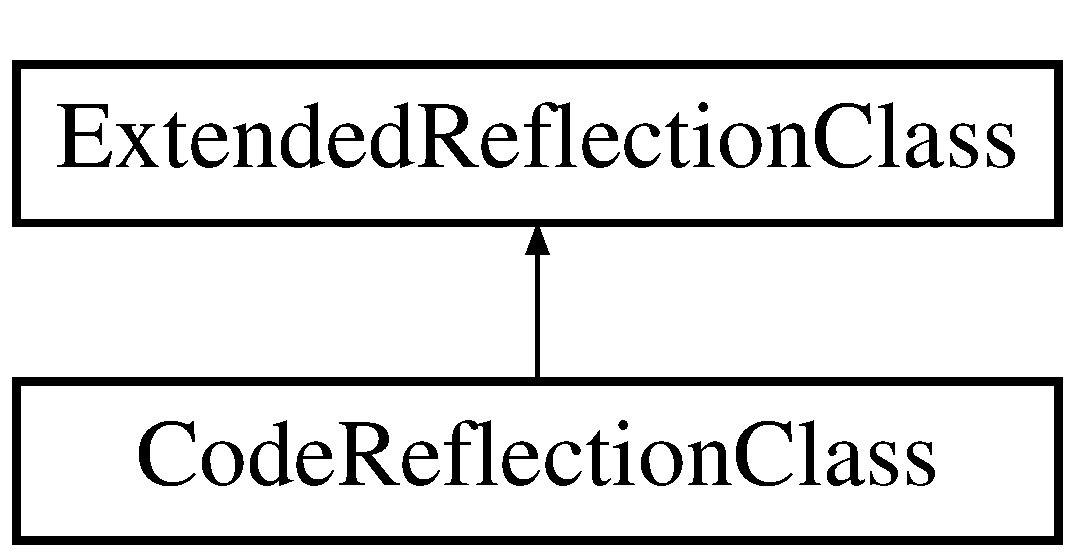
\includegraphics[height=3cm]{class_code_reflection_class}
\end{center}
\end{figure}
\subsection*{Public Member Functions}
\begin{CompactItemize}
\item 
\hyperlink{class_code_reflection_class_4df49469648d1e8de92c18bb8ac40b1b}{\_\-\_\-construct} (\$strClassName, \$strEvalContent=\char`\"{}\char`\"{})
\item 
\hyperlink{class_code_reflection_class_b8f8ee56588ebf5091c288e44ebdfaf4}{getClassName} ()
\item 
\hyperlink{class_code_reflection_class_2614df64646ac71b70b1e1074258052b}{getNamespace} ()
\item 
\hyperlink{class_code_reflection_class_a56c2962a9dd11f78bdafb688f9cd8fa}{getRealClassName} ()
\item 
\hyperlink{class_code_reflection_class_98b016c8a77c458803bb6905c89c914b}{createClassDefinitionCode} ()
\item 
\hyperlink{class_code_reflection_class_72b25801f6d2c909af2ee16b2b51ab8f}{createAttributesDefinitionCode} ()
\item 
\hyperlink{class_code_reflection_class_c2d23f8614e24561b794d5031001eaf8}{createMethodsDefinitionCode} ()
\item 
\hyperlink{class_code_reflection_class_b5e24da53b4a0d0848b18c1e832f47ff}{getCode} ()
\end{CompactItemize}
\subsection*{Protected Member Functions}
\begin{CompactItemize}
\item 
\hyperlink{class_code_reflection_class_6b56ec198bc6a5b5a72076e4e7c19e29}{createExtendedReflectionClass} (ReflectionClass \$objOriginalReflectionClass)
\item 
\hyperlink{class_code_reflection_class_bce271bf4f7b77b8b11986404241ab5c}{createExtendedReflectionProperty} (ReflectionProperty \$objOriginalReflectionProperty)
\item 
\hyperlink{class_code_reflection_class_ec7c1d4b204b6e3a6291d3b867afb688}{createExtendedReflectionMethod} (ReflectionMethod \$objOriginalReflectionMethod)
\end{CompactItemize}


\subsection{Detailed Description}
Code reflection class it is a class what is a extension of the php reflection with improvments to show the php code of the reflected class

With this class you can see the code of some class, method, attribute just as it is and extending this class you can create a similary class of the original one.

This class can be used to debug, detail of some execution or stack and to code instrumentation.

\begin{Desc}
\item[Author:]Thiago Henrique Ramos da Mata $<$\href{mailto:thiago.henrique.mata@gmail.com}{\tt thiago.henrique.mata@gmail.com}$>$ ' $\ast$ \end{Desc}


\subsection{Constructor \& Destructor Documentation}
\hypertarget{class_code_reflection_class_4df49469648d1e8de92c18bb8ac40b1b}{
\index{CodeReflectionClass@{CodeReflectionClass}!\_\-\_\-construct@{\_\-\_\-construct}}
\index{\_\-\_\-construct@{\_\-\_\-construct}!CodeReflectionClass@{CodeReflectionClass}}
\subsubsection[{\_\-\_\-construct}]{\setlength{\rightskip}{0pt plus 5cm}\_\-\_\-construct (\$ {\em strClassName}, \/  \$ {\em strEvalContent} = {\tt \char`\"{}\char`\"{}})}}
\label{class_code_reflection_class_4df49469648d1e8de92c18bb8ac40b1b}


Construct the Code Reflection of the class.

It must receive the eval content if the class it was created into a eval command.

\begin{Desc}
\item[Parameters:]
\begin{description}
\item[{\em string}]\$strClassName \item[{\em string}]\$strEvalContent \end{description}
\end{Desc}


Reimplemented in \hyperlink{class_code_instrumentation_class_4df49469648d1e8de92c18bb8ac40b1b}{CodeInstrumentationClass}.

\begin{Code}\begin{verbatim}33     {
34         parent::__construct( $strClassName );
35         if( $strEvalContent != "" )
36         {
37             new CodeReflectionFile( $this->getFileName() , $strEvalContent , false );
38         }
39     }
\end{verbatim}
\end{Code}




\subsection{Member Function Documentation}
\hypertarget{class_code_reflection_class_72b25801f6d2c909af2ee16b2b51ab8f}{
\index{CodeReflectionClass@{CodeReflectionClass}!createAttributesDefinitionCode@{createAttributesDefinitionCode}}
\index{createAttributesDefinitionCode@{createAttributesDefinitionCode}!CodeReflectionClass@{CodeReflectionClass}}
\subsubsection[{createAttributesDefinitionCode}]{\setlength{\rightskip}{0pt plus 5cm}createAttributesDefinitionCode ()}}
\label{class_code_reflection_class_72b25801f6d2c909af2ee16b2b51ab8f}


Create a php attribute definition code

\begin{Desc}
\item[Returns:]string code of attribute \end{Desc}


\begin{Code}\begin{verbatim}114         {
115                 $strCode = "";
116                 $arrProperties = $this->getProperties();
117                 foreach( $arrProperties as $objReflectionProperty )
118                 {
119                         /*@var $objReflectionProperty CodeReflectionProperty */
120                         $strCode .= $objReflectionProperty->getCode();
121                 }
122         $arrConstants = $this->getConstants();
123                 foreach( $arrConstants as $strKey => $mixValue )
124                 {
125                         /*@var $objReflectionProperty CodeReflectionProperty */
126                         $strCode .= "const " . $strKey . ' = ' . var_export( $mixValue , true ) . ";\n";
127                 }
128                 return $strCode;
129         }
\end{verbatim}
\end{Code}


\hypertarget{class_code_reflection_class_98b016c8a77c458803bb6905c89c914b}{
\index{CodeReflectionClass@{CodeReflectionClass}!createClassDefinitionCode@{createClassDefinitionCode}}
\index{createClassDefinitionCode@{createClassDefinitionCode}!CodeReflectionClass@{CodeReflectionClass}}
\subsubsection[{createClassDefinitionCode}]{\setlength{\rightskip}{0pt plus 5cm}createClassDefinitionCode ()}}
\label{class_code_reflection_class_98b016c8a77c458803bb6905c89c914b}


Create a php class definition code

\begin{Desc}
\item[Returns:]string code of class creation \end{Desc}


\begin{Code}\begin{verbatim}87         {
88                 $strCode = "";
89                 $strCode .= " class " . $this->getClassName();
90                 if( $this->getParentClass() != "" )
91                 {
92                         $strCode .= " extends " . $this->getParentClass()->getClassName();
93                 }
94                 if( sizeof( $this->getInterfaceNames() ) > 0)
95                 {
96                         $arrInterfacesClassName = array();
97                         $arrInterfaces = $this->getInterfaces();
98                         foreach(  $arrInterfaces as $objInterfaces )
99                         {
100                                 $arrInterfacesClassName[] = $objInterfaces->getClassName();
101                         }
102                         $strCode .= " implements " . implode( ", " , $arrInterfacesClassName );
103                 }
104                 $strCode .= "\n";
105                 return $strCode;
106         }
\end{verbatim}
\end{Code}


\hypertarget{class_code_reflection_class_6b56ec198bc6a5b5a72076e4e7c19e29}{
\index{CodeReflectionClass@{CodeReflectionClass}!createExtendedReflectionClass@{createExtendedReflectionClass}}
\index{createExtendedReflectionClass@{createExtendedReflectionClass}!CodeReflectionClass@{CodeReflectionClass}}
\subsubsection[{createExtendedReflectionClass}]{\setlength{\rightskip}{0pt plus 5cm}createExtendedReflectionClass (ReflectionClass \$ {\em objOriginalReflectionClass})\hspace{0.3cm}{\tt  \mbox{[}protected\mbox{]}}}}
\label{class_code_reflection_class_6b56ec198bc6a5b5a72076e4e7c19e29}


Make the recursive calls and indirectly call return the extended reflection object and not a native reflection class.

\begin{Desc}
\item[See also:]ExtendedReflectionClass::createExtendedReflectionClass( ReflectionClass ) \end{Desc}
\begin{Desc}
\item[Parameters:]
\begin{description}
\item[{\em ReflectionClass}]\$objOriginalReflectionClass \end{description}
\end{Desc}
\begin{Desc}
\item[Returns:]\hyperlink{class_code_reflection_class}{CodeReflectionClass} \end{Desc}


Reimplemented from \hyperlink{class_extended_reflection_class_6b56ec198bc6a5b5a72076e4e7c19e29}{ExtendedReflectionClass}.

Reimplemented in \hyperlink{class_code_instrumentation_class_6b56ec198bc6a5b5a72076e4e7c19e29}{CodeInstrumentationClass}.

\begin{Code}\begin{verbatim}198         {
199                 return new CodeReflectionClass( $objOriginalReflectionClass->getName() );
200         }
\end{verbatim}
\end{Code}


\hypertarget{class_code_reflection_class_ec7c1d4b204b6e3a6291d3b867afb688}{
\index{CodeReflectionClass@{CodeReflectionClass}!createExtendedReflectionMethod@{createExtendedReflectionMethod}}
\index{createExtendedReflectionMethod@{createExtendedReflectionMethod}!CodeReflectionClass@{CodeReflectionClass}}
\subsubsection[{createExtendedReflectionMethod}]{\setlength{\rightskip}{0pt plus 5cm}createExtendedReflectionMethod (ReflectionMethod \$ {\em objOriginalReflectionMethod})\hspace{0.3cm}{\tt  \mbox{[}protected\mbox{]}}}}
\label{class_code_reflection_class_ec7c1d4b204b6e3a6291d3b867afb688}


Make the recursive calls and indirectly call return the extended reflection object and not a native reflection method.

\begin{Desc}
\item[See also:]ExtendedReflectionClass::createExtendedReflectionMethod( ReflectionMethod ) \end{Desc}
\begin{Desc}
\item[Parameters:]
\begin{description}
\item[{\em ReflectionMethod}]\$objOriginalReflectionClass \end{description}
\end{Desc}
\begin{Desc}
\item[Returns:]\hyperlink{class_code_reflection_method}{CodeReflectionMethod} \end{Desc}


Reimplemented from \hyperlink{class_extended_reflection_class_ec7c1d4b204b6e3a6291d3b867afb688}{ExtendedReflectionClass}.

Reimplemented in \hyperlink{class_code_instrumentation_class_ec7c1d4b204b6e3a6291d3b867afb688}{CodeInstrumentationClass}.

\begin{Code}\begin{verbatim}224         {
225                 return new CodeReflectionMethod( $this->getName() , $objOriginalReflectionMethod->getName() );
226         }
\end{verbatim}
\end{Code}


\hypertarget{class_code_reflection_class_bce271bf4f7b77b8b11986404241ab5c}{
\index{CodeReflectionClass@{CodeReflectionClass}!createExtendedReflectionProperty@{createExtendedReflectionProperty}}
\index{createExtendedReflectionProperty@{createExtendedReflectionProperty}!CodeReflectionClass@{CodeReflectionClass}}
\subsubsection[{createExtendedReflectionProperty}]{\setlength{\rightskip}{0pt plus 5cm}createExtendedReflectionProperty (ReflectionProperty \$ {\em objOriginalReflectionProperty})\hspace{0.3cm}{\tt  \mbox{[}protected\mbox{]}}}}
\label{class_code_reflection_class_bce271bf4f7b77b8b11986404241ab5c}


Make the recursive calls and indirectly call return the extended reflection object and not a native reflection property.

\begin{Desc}
\item[See also:]ExtendedReflectionClass::createExtendedReflectionProperty( ReflectionProperty ) \end{Desc}
\begin{Desc}
\item[Parameters:]
\begin{description}
\item[{\em ReflectionProperty}]\$objOriginalReflectionClass \end{description}
\end{Desc}
\begin{Desc}
\item[Returns:]\hyperlink{class_code_reflection_property}{CodeReflectionProperty} \end{Desc}


Reimplemented from \hyperlink{class_extended_reflection_class_bce271bf4f7b77b8b11986404241ab5c}{ExtendedReflectionClass}.

Reimplemented in \hyperlink{class_code_instrumentation_class_bce271bf4f7b77b8b11986404241ab5c}{CodeInstrumentationClass}.

\begin{Code}\begin{verbatim}211         {
212                 return new CodeReflectionProperty( $this->getName() , $objOriginalReflectionProperty->getName() );
213         }
\end{verbatim}
\end{Code}


\hypertarget{class_code_reflection_class_c2d23f8614e24561b794d5031001eaf8}{
\index{CodeReflectionClass@{CodeReflectionClass}!createMethodsDefinitionCode@{createMethodsDefinitionCode}}
\index{createMethodsDefinitionCode@{createMethodsDefinitionCode}!CodeReflectionClass@{CodeReflectionClass}}
\subsubsection[{createMethodsDefinitionCode}]{\setlength{\rightskip}{0pt plus 5cm}createMethodsDefinitionCode ()}}
\label{class_code_reflection_class_c2d23f8614e24561b794d5031001eaf8}


Create a php method definiton code

\begin{Desc}
\item[Returns:]string code of method \end{Desc}


Reimplemented in \hyperlink{class_code_instrumentation_class_c2d23f8614e24561b794d5031001eaf8}{CodeInstrumentationClass}.

\begin{Code}\begin{verbatim}137         {
138                 $strCode = "";
139                 $arrMethods = $this->getMethods();
140                 foreach( $arrMethods as $objReflectionMethod )
141                 {
142                         /*@var $objReflectionMethod CodeReflectionMethod */
143             if( $objReflectionMethod->getDeclaringClass()->getRealClassName() == $this->getRealClassName())
144                         {
145                 if( !$this->isInterface() )
146                 {
147                     $strCode .= $objReflectionMethod->getCode();
148                 }
149                 else
150                 {
151                     $strCode .= $objReflectionMethod->createMethodHeaderCode();
152                 }
153             }
154                 }
155                 return $strCode;
156         }
\end{verbatim}
\end{Code}


\hypertarget{class_code_reflection_class_b8f8ee56588ebf5091c288e44ebdfaf4}{
\index{CodeReflectionClass@{CodeReflectionClass}!getClassName@{getClassName}}
\index{getClassName@{getClassName}!CodeReflectionClass@{CodeReflectionClass}}
\subsubsection[{getClassName}]{\setlength{\rightskip}{0pt plus 5cm}getClassName ()}}
\label{class_code_reflection_class_b8f8ee56588ebf5091c288e44ebdfaf4}


Get the class name

\begin{Desc}
\item[Returns:]string \end{Desc}


Reimplemented in \hyperlink{class_code_instrumentation_class_b8f8ee56588ebf5091c288e44ebdfaf4}{CodeInstrumentationClass}.

\begin{Code}\begin{verbatim}47         {
48         $strName = parent::getName();
49         $arrName = explode( "::" ,$strName) ;
50                 return array_pop( $arrName );
51         }
\end{verbatim}
\end{Code}


\hypertarget{class_code_reflection_class_b5e24da53b4a0d0848b18c1e832f47ff}{
\index{CodeReflectionClass@{CodeReflectionClass}!getCode@{getCode}}
\index{getCode@{getCode}!CodeReflectionClass@{CodeReflectionClass}}
\subsubsection[{getCode}]{\setlength{\rightskip}{0pt plus 5cm}getCode ()}}
\label{class_code_reflection_class_b5e24da53b4a0d0848b18c1e832f47ff}


Create the code of the reflected object

\begin{Desc}
\item[See also:]\hyperlink{class_code_reflection_class_98b016c8a77c458803bb6905c89c914b}{CodeReflectionClass::createClassDefinitionCode} 

CodeReflectionClass::createInterfaceDefinitionCode 

\hyperlink{class_code_reflection_class_72b25801f6d2c909af2ee16b2b51ab8f}{CodeReflectionClass::createAttributesDefinitionCode} 

\hyperlink{class_code_reflection_class_c2d23f8614e24561b794d5031001eaf8}{CodeReflectionClass::createMethodsDefinitionCode} \end{Desc}
\begin{Desc}
\item[Returns:]string code of the reflected object \end{Desc}


\begin{Code}\begin{verbatim}168         {
169         $strCode = "";
170         if( !$this->isInterface() )
171         {
172             $strCode .= $this->createClassDefinitionCode();
173             $strCode .= "{\n";
174             $strCode .= $this->createAttributesDefinitionCode();
175             $strCode .= $this->createMethodsDefinitionCode();
176             $strCode .= "\n}\n";
177         }
178         else
179         {
180             $strCode .= $this->createInterfaceDefinitionCode();
181             $strCode .= "{\n";
182             $strCode .= $this->createAttributesDefinitionCode();
183             $strCode .= $this->createMethodsDefinitionCode();
184             $strCode .= "\n}\n";
185         }
186                 return $strCode;
187         }
\end{verbatim}
\end{Code}


\hypertarget{class_code_reflection_class_2614df64646ac71b70b1e1074258052b}{
\index{CodeReflectionClass@{CodeReflectionClass}!getNamespace@{getNamespace}}
\index{getNamespace@{getNamespace}!CodeReflectionClass@{CodeReflectionClass}}
\subsubsection[{getNamespace}]{\setlength{\rightskip}{0pt plus 5cm}getNamespace ()}}
\label{class_code_reflection_class_2614df64646ac71b70b1e1074258052b}


Get the namespace name

\begin{Desc}
\item[Returns:]string \end{Desc}


\begin{Code}\begin{verbatim}59         {
60         $strName = parent::getName();
61         $arrName = explode( "::" ,$strName) ;
62                 return array_shift( $arrName );
63         }
\end{verbatim}
\end{Code}


\hypertarget{class_code_reflection_class_a56c2962a9dd11f78bdafb688f9cd8fa}{
\index{CodeReflectionClass@{CodeReflectionClass}!getRealClassName@{getRealClassName}}
\index{getRealClassName@{getRealClassName}!CodeReflectionClass@{CodeReflectionClass}}
\subsubsection[{getRealClassName}]{\setlength{\rightskip}{0pt plus 5cm}getRealClassName ()\hspace{0.3cm}{\tt  \mbox{[}final\mbox{]}}}}
\label{class_code_reflection_class_a56c2962a9dd11f78bdafb688f9cd8fa}


A version of the get class name what cannot be replaced.

Should be used when the execution need the real original class name

\begin{Desc}
\item[Returns:]string \end{Desc}


\begin{Code}\begin{verbatim}75     {
76         $strName = ExtendedReflectionClass::getName();
77         $arrName = explode( "::" ,$strName) ;
78                 return array_pop( $arrName );
79     }
\end{verbatim}
\end{Code}




The documentation for this class was generated from the following file:\begin{CompactItemize}
\item 
components/codeReflection/\hyperlink{_code_reflection_class_8class_8php}{CodeReflectionClass.class.php}\end{CompactItemize}

\hypertarget{class_code_reflection_exception}{
\section{CodeReflectionException Class Reference}
\label{class_code_reflection_exception}\index{CodeReflectionException@{CodeReflectionException}}
}


\subsection{Detailed Description}
Code Reflection Exception

\begin{Desc}
\item[Author:]Thiago Henrique Ramos da Mata $<$\href{mailto:thiago.henrique.mata@gmail.com}{\tt thiago.henrique.mata@gmail.com}$>$ \end{Desc}


The documentation for this class was generated from the following file:\begin{CompactItemize}
\item 
components/codeReflection/\hyperlink{_code_reflection_exception_8class_8php}{CodeReflectionException.class.php}\end{CompactItemize}

\hypertarget{class_code_reflection_file}{
\section{CodeReflectionFile Class Reference}
\label{class_code_reflection_file}\index{CodeReflectionFile@{CodeReflectionFile}}
}
\subsection*{Public Member Functions}
\begin{CompactItemize}
\item 
\hyperlink{class_code_reflection_file_85d5cd6390afa77ea3d3e67b8ebc762d}{\_\-\_\-construct} (\$strFileName, \$strFileContent=\char`\"{}\char`\"{}, \$boolRealFile=true)
\item 
\hyperlink{class_code_reflection_file_17c133a6bfc041953b6054ca6137c1e9}{setFileName} (\$strFileName)
\item 
\hyperlink{class_code_reflection_file_fd1320273fcd2bbeada22a40d33974ae}{getFileName} ()
\item 
\hyperlink{class_code_reflection_file_8bd4ac0c26519528027a9f2a2840ce77}{setFileContent} (\$strFileContent)
\item 
\hyperlink{class_code_reflection_file_f87150d5f818f1b92d30db63dfdf966a}{getFileContent} ()
\item 
\hyperlink{class_code_reflection_file_1c6e129f863511fd326ccf7a13d64c5a}{getArrFileContent} ()
\item 
\hyperlink{class_code_reflection_file_d5d0f670cbe1798cb50ad67ae37a9164}{getFileBit} (\$intLineStart, \$intLineEnds)
\item 
\hyperlink{class_code_reflection_file_995a74eebd5970a3bbe99c27a231600a}{isRealFile} ()
\end{CompactItemize}
\subsection*{Static Public Member Functions}
\begin{CompactItemize}
\item 
static \hyperlink{class_code_reflection_file_43822c529c08e8f126ab454b209fc31f}{getCodeInstrFileName} (\$strFileName)
\end{CompactItemize}
\subsection*{Protected Attributes}
\begin{CompactItemize}
\item 
\hyperlink{class_code_reflection_file_47606edf90d11273c6b4a4b319bc42c7}{\$strFileName}
\item 
\hyperlink{class_code_reflection_file_ce8c257c3c8d9148294d0b6f3493c2ba}{\$arrFileContent}
\item 
\hyperlink{class_code_reflection_file_9e00721eed14d115918aaba925005394}{\$boolRealFile}
\end{CompactItemize}
\subsection*{Static Protected Attributes}
\begin{CompactItemize}
\item 
static \hyperlink{class_code_reflection_file_019a4ce9092e6ea5f4e51e131e3a0352}{\$arrInstances} = array()
\end{CompactItemize}


\subsection{Constructor \& Destructor Documentation}
\hypertarget{class_code_reflection_file_85d5cd6390afa77ea3d3e67b8ebc762d}{
\index{CodeReflectionFile@{CodeReflectionFile}!\_\-\_\-construct@{\_\-\_\-construct}}
\index{\_\-\_\-construct@{\_\-\_\-construct}!CodeReflectionFile@{CodeReflectionFile}}
\subsubsection[{\_\-\_\-construct}]{\setlength{\rightskip}{0pt plus 5cm}CodeReflectionFile::\_\-\_\-construct (\$ {\em strFileName}, \/  \$ {\em strFileContent} = {\tt \char`\"{}\char`\"{}}, \/  \$ {\em boolRealFile} = {\tt true})}}
\label{class_code_reflection_file_85d5cd6390afa77ea3d3e67b8ebc762d}


Create the Code Reflection File

\begin{Desc}
\item[See also:]\hyperlink{class_code_reflection_file_019a4ce9092e6ea5f4e51e131e3a0352}{CodeReflectionFile::\$arrInstances} 

CodeReflectionFile::setFileName( string ) 

CodeReflectionFile::setFileContent( string ) \end{Desc}
\begin{Desc}
\item[Parameters:]
\begin{description}
\item[{\em string}]\$strFileName file name \item[{\em string}]\$strFileContent file content \item[{\em boolean}]\$boolRealFile if is a real file or not \end{description}
\end{Desc}


\subsection{Member Function Documentation}
\hypertarget{class_code_reflection_file_1c6e129f863511fd326ccf7a13d64c5a}{
\index{CodeReflectionFile@{CodeReflectionFile}!getArrFileContent@{getArrFileContent}}
\index{getArrFileContent@{getArrFileContent}!CodeReflectionFile@{CodeReflectionFile}}
\subsubsection[{getArrFileContent}]{\setlength{\rightskip}{0pt plus 5cm}CodeReflectionFile::getArrFileContent ()}}
\label{class_code_reflection_file_1c6e129f863511fd326ccf7a13d64c5a}


Get the array of lines with the code file content

Set the code file content and return itselft.

\begin{Desc}
\item[See also:]CodeReflectionFile-$>$arrFileContent 

CodeReflectionFile::setFileContent( string ) 

\hyperlink{class_code_reflection_file_f87150d5f818f1b92d30db63dfdf966a}{CodeReflectionFile::getFileContent()} \end{Desc}
\begin{Desc}
\item[Returns:]string\mbox{[}\mbox{]} array of file content \end{Desc}
\hypertarget{class_code_reflection_file_43822c529c08e8f126ab454b209fc31f}{
\index{CodeReflectionFile@{CodeReflectionFile}!getCodeInstrFileName@{getCodeInstrFileName}}
\index{getCodeInstrFileName@{getCodeInstrFileName}!CodeReflectionFile@{CodeReflectionFile}}
\subsubsection[{getCodeInstrFileName}]{\setlength{\rightskip}{0pt plus 5cm}static CodeReflectionFile::getCodeInstrFileName (\$ {\em strFileName})\hspace{0.3cm}{\tt  \mbox{[}static\mbox{]}}}}
\label{class_code_reflection_file_43822c529c08e8f126ab454b209fc31f}


Get The File by Name

Search into all object files saved and return that one have the searched name

\begin{Desc}
\item[See also:]CodeReflectionFile-$>$arrInstances \end{Desc}
\begin{Desc}
\item[Parameters:]
\begin{description}
\item[{\em string}]\$strFileName \end{description}
\end{Desc}
\begin{Desc}
\item[Returns:]\hyperlink{class_code_reflection_file}{CodeReflectionFile} \end{Desc}
\hypertarget{class_code_reflection_file_d5d0f670cbe1798cb50ad67ae37a9164}{
\index{CodeReflectionFile@{CodeReflectionFile}!getFileBit@{getFileBit}}
\index{getFileBit@{getFileBit}!CodeReflectionFile@{CodeReflectionFile}}
\subsubsection[{getFileBit}]{\setlength{\rightskip}{0pt plus 5cm}CodeReflectionFile::getFileBit (\$ {\em intLineStart}, \/  \$ {\em intLineEnds})}}
\label{class_code_reflection_file_d5d0f670cbe1798cb50ad67ae37a9164}


Get a slice, a streck, a bit of the content of the file receiving the first and last line of the slice wish.

\begin{Desc}
\item[See also:]CodeReflectionFile::setFileContent( string ) 

CodeReflectionFile-$>$arrFileContent 

CodeReflectionFile-$>$arrFileContent \end{Desc}
\begin{Desc}
\item[Parameters:]
\begin{description}
\item[{\em integer}]\$intLineStart first line of the content \item[{\em integer}]\$intLineEnds last line of the content \end{description}
\end{Desc}
\begin{Desc}
\item[Returns:]string code content \end{Desc}
\hypertarget{class_code_reflection_file_f87150d5f818f1b92d30db63dfdf966a}{
\index{CodeReflectionFile@{CodeReflectionFile}!getFileContent@{getFileContent}}
\index{getFileContent@{getFileContent}!CodeReflectionFile@{CodeReflectionFile}}
\subsubsection[{getFileContent}]{\setlength{\rightskip}{0pt plus 5cm}CodeReflectionFile::getFileContent ()}}
\label{class_code_reflection_file_f87150d5f818f1b92d30db63dfdf966a}


Get the file content

\begin{Desc}
\item[See also:]CodeReflectionFile-$>$arrFileContent 

CodeReflectionFile::setFileContent( string ) \end{Desc}
\begin{Desc}
\item[Returns:]string file content \end{Desc}
\hypertarget{class_code_reflection_file_fd1320273fcd2bbeada22a40d33974ae}{
\index{CodeReflectionFile@{CodeReflectionFile}!getFileName@{getFileName}}
\index{getFileName@{getFileName}!CodeReflectionFile@{CodeReflectionFile}}
\subsubsection[{getFileName}]{\setlength{\rightskip}{0pt plus 5cm}CodeReflectionFile::getFileName ()}}
\label{class_code_reflection_file_fd1320273fcd2bbeada22a40d33974ae}


Get the file name

\begin{Desc}
\item[See also:]CodeReflectionFile::setFileName( string ) 

CodeReflectionFile-$>$strFileName \end{Desc}
\begin{Desc}
\item[Returns:]string file name \end{Desc}
\hypertarget{class_code_reflection_file_995a74eebd5970a3bbe99c27a231600a}{
\index{CodeReflectionFile@{CodeReflectionFile}!isRealFile@{isRealFile}}
\index{isRealFile@{isRealFile}!CodeReflectionFile@{CodeReflectionFile}}
\subsubsection[{isRealFile}]{\setlength{\rightskip}{0pt plus 5cm}CodeReflectionFile::isRealFile ()}}
\label{class_code_reflection_file_995a74eebd5970a3bbe99c27a231600a}


Returns if the file it is a real file

\begin{Desc}
\item[See also:]CodeReflectionFile-$>$boolRealFile \end{Desc}
\begin{Desc}
\item[Returns:]boolean {\tt true} if is a real file {\tt false} if not \end{Desc}
\hypertarget{class_code_reflection_file_8bd4ac0c26519528027a9f2a2840ce77}{
\index{CodeReflectionFile@{CodeReflectionFile}!setFileContent@{setFileContent}}
\index{setFileContent@{setFileContent}!CodeReflectionFile@{CodeReflectionFile}}
\subsubsection[{setFileContent}]{\setlength{\rightskip}{0pt plus 5cm}CodeReflectionFile::setFileContent (\$ {\em strFileContent})}}
\label{class_code_reflection_file_8bd4ac0c26519528027a9f2a2840ce77}


Set the code Reflection file content

Set the code Reflection file content and return itselft.

\begin{Desc}
\item[See also:]CodeReflectionFile-$>$arrFileContent \end{Desc}
\begin{Desc}
\item[Parameters:]
\begin{description}
\item[{\em string}]\$strFileContent file content \end{description}
\end{Desc}
\begin{Desc}
\item[Returns:]\hyperlink{class_code_reflection_file}{CodeReflectionFile} me \end{Desc}
\hypertarget{class_code_reflection_file_17c133a6bfc041953b6054ca6137c1e9}{
\index{CodeReflectionFile@{CodeReflectionFile}!setFileName@{setFileName}}
\index{setFileName@{setFileName}!CodeReflectionFile@{CodeReflectionFile}}
\subsubsection[{setFileName}]{\setlength{\rightskip}{0pt plus 5cm}CodeReflectionFile::setFileName (\$ {\em strFileName})}}
\label{class_code_reflection_file_17c133a6bfc041953b6054ca6137c1e9}


Set the file name

\begin{Desc}
\item[See also:]\hyperlink{class_code_reflection_file_fd1320273fcd2bbeada22a40d33974ae}{CodeReflectionFile::getFileName()} 

CodeReflectionFile-$>$strFileName \end{Desc}
\begin{Desc}
\item[Parameters:]
\begin{description}
\item[{\em string}]\$strFileName file name \end{description}
\end{Desc}
\begin{Desc}
\item[Returns:]\hyperlink{class_code_reflection_file}{CodeReflectionFile} me \end{Desc}


\subsection{Member Data Documentation}
\hypertarget{class_code_reflection_file_ce8c257c3c8d9148294d0b6f3493c2ba}{
\index{CodeReflectionFile@{CodeReflectionFile}!\$arrFileContent@{\$arrFileContent}}
\index{\$arrFileContent@{\$arrFileContent}!CodeReflectionFile@{CodeReflectionFile}}
\subsubsection[{\$arrFileContent}]{\setlength{\rightskip}{0pt plus 5cm}CodeReflectionFile::\$arrFileContent\hspace{0.3cm}{\tt  \mbox{[}protected\mbox{]}}}}
\label{class_code_reflection_file_ce8c257c3c8d9148294d0b6f3493c2ba}


\hypertarget{class_code_reflection_file_019a4ce9092e6ea5f4e51e131e3a0352}{
\index{CodeReflectionFile@{CodeReflectionFile}!\$arrInstances@{\$arrInstances}}
\index{\$arrInstances@{\$arrInstances}!CodeReflectionFile@{CodeReflectionFile}}
\subsubsection[{\$arrInstances}]{\setlength{\rightskip}{0pt plus 5cm}CodeReflectionFile::\$arrInstances = array()\hspace{0.3cm}{\tt  \mbox{[}static, protected\mbox{]}}}}
\label{class_code_reflection_file_019a4ce9092e6ea5f4e51e131e3a0352}


\hypertarget{class_code_reflection_file_9e00721eed14d115918aaba925005394}{
\index{CodeReflectionFile@{CodeReflectionFile}!\$boolRealFile@{\$boolRealFile}}
\index{\$boolRealFile@{\$boolRealFile}!CodeReflectionFile@{CodeReflectionFile}}
\subsubsection[{\$boolRealFile}]{\setlength{\rightskip}{0pt plus 5cm}CodeReflectionFile::\$boolRealFile\hspace{0.3cm}{\tt  \mbox{[}protected\mbox{]}}}}
\label{class_code_reflection_file_9e00721eed14d115918aaba925005394}


\hypertarget{class_code_reflection_file_47606edf90d11273c6b4a4b319bc42c7}{
\index{CodeReflectionFile@{CodeReflectionFile}!\$strFileName@{\$strFileName}}
\index{\$strFileName@{\$strFileName}!CodeReflectionFile@{CodeReflectionFile}}
\subsubsection[{\$strFileName}]{\setlength{\rightskip}{0pt plus 5cm}CodeReflectionFile::\$strFileName\hspace{0.3cm}{\tt  \mbox{[}protected\mbox{]}}}}
\label{class_code_reflection_file_47606edf90d11273c6b4a4b319bc42c7}




The documentation for this class was generated from the following file:\begin{CompactItemize}
\item 
components/codeReflection/\hyperlink{_code_reflection_file_8class_8php}{CodeReflectionFile.class.php}\end{CompactItemize}

\hypertarget{class_code_reflection_function}{
\section{CodeReflectionFunction Class Reference}
\label{class_code_reflection_function}\index{CodeReflectionFunction@{CodeReflectionFunction}}
}
Inheritance diagram for CodeReflectionFunction::\begin{figure}[H]
\begin{center}
\leavevmode
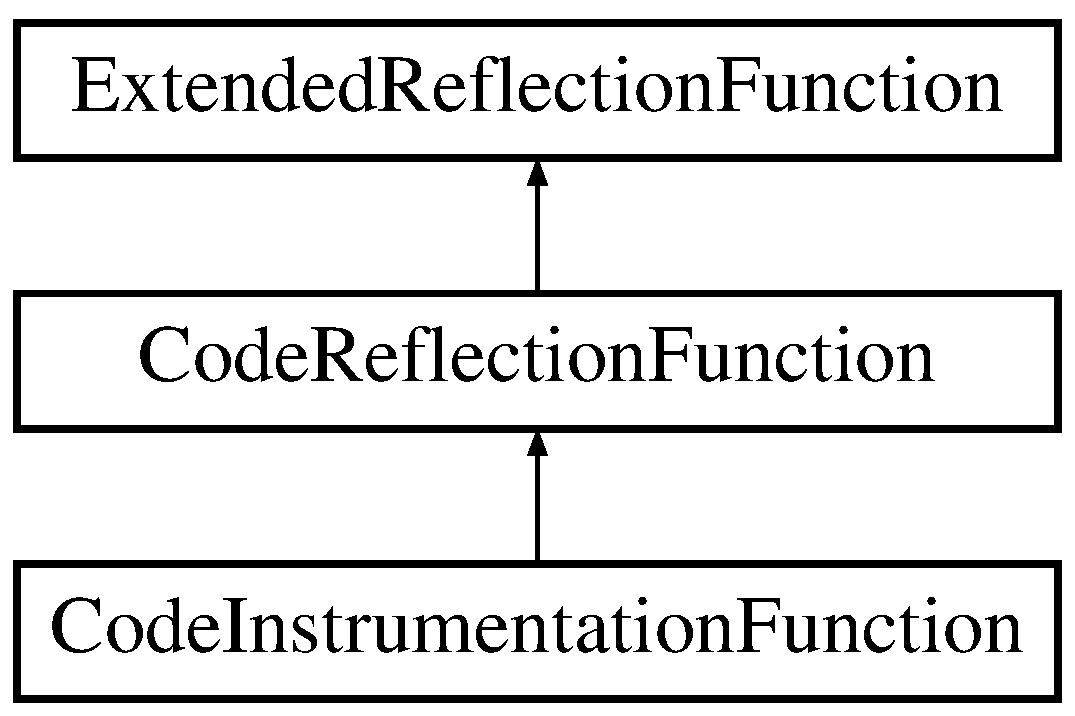
\includegraphics[height=3cm]{class_code_reflection_function}
\end{center}
\end{figure}
\subsection*{Public Member Functions}
\begin{CompactItemize}
\item 
\hyperlink{class_code_reflection_function_eb645ce888eda144d361ccfd14eb9878}{getCode} ()
\item 
\hyperlink{class_code_reflection_function_11b5048c516be3731737308e5cddef79}{getCodeContent} ()
\item 
\hyperlink{class_code_reflection_function_f239516580c5c5e66c02bbe6c55d2f2f}{createFunctionHeaderCode} ()
\end{CompactItemize}
\subsection*{Protected Member Functions}
\begin{CompactItemize}
\item 
\hyperlink{class_code_reflection_function_7ce14d3f6e8579332f226d85fb439b80}{createExtendedReflectionParameter} (ReflectionParameter \$objReflectionParameter)
\item 
\hyperlink{class_code_reflection_function_003298f670f7915ad557ad10b777e0bb}{createParametersCode} ()
\item 
\hyperlink{class_code_reflection_function_3ea191f1a3ff9fa0b3505327e635d306}{createFunctionContentCode} ()
\end{CompactItemize}


\subsection{Member Function Documentation}
\hypertarget{class_code_reflection_function_7ce14d3f6e8579332f226d85fb439b80}{
\index{CodeReflectionFunction@{CodeReflectionFunction}!createExtendedReflectionParameter@{createExtendedReflectionParameter}}
\index{createExtendedReflectionParameter@{createExtendedReflectionParameter}!CodeReflectionFunction@{CodeReflectionFunction}}
\subsubsection[{createExtendedReflectionParameter}]{\setlength{\rightskip}{0pt plus 5cm}CodeReflectionFunction::createExtendedReflectionParameter (ReflectionParameter \$ {\em objReflectionParameter})\hspace{0.3cm}{\tt  \mbox{[}protected\mbox{]}}}}
\label{class_code_reflection_function_7ce14d3f6e8579332f226d85fb439b80}


Make the reflection parameter link return a code reflection parameter

\begin{Desc}
\item[See also:]\hyperlink{class_extended_reflection_function_de07ccd452e54a7c8878fc20d215831e}{ExtendedReflectionFunction::createExtendedReflectionParameter()} \end{Desc}
\begin{Desc}
\item[Parameters:]
\begin{description}
\item[{\em ReflectionParameter}]\$objReflectionParameter \end{description}
\end{Desc}
\begin{Desc}
\item[Returns:]\hyperlink{class_code_reflection_parameter}{CodeReflectionParameter} \end{Desc}


Reimplemented from \hyperlink{class_extended_reflection_function_de07ccd452e54a7c8878fc20d215831e}{ExtendedReflectionFunction}.

Reimplemented in \hyperlink{class_code_instrumentation_function_3d95491ac661050b8e8ecedfaf3c8359}{CodeInstrumentationFunction}.\hypertarget{class_code_reflection_function_3ea191f1a3ff9fa0b3505327e635d306}{
\index{CodeReflectionFunction@{CodeReflectionFunction}!createFunctionContentCode@{createFunctionContentCode}}
\index{createFunctionContentCode@{createFunctionContentCode}!CodeReflectionFunction@{CodeReflectionFunction}}
\subsubsection[{createFunctionContentCode}]{\setlength{\rightskip}{0pt plus 5cm}CodeReflectionFunction::createFunctionContentCode ()\hspace{0.3cm}{\tt  \mbox{[}protected\mbox{]}}}}
\label{class_code_reflection_function_3ea191f1a3ff9fa0b3505327e635d306}


Creater the function content

\begin{Desc}
\item[Returns:]string \end{Desc}
\hypertarget{class_code_reflection_function_f239516580c5c5e66c02bbe6c55d2f2f}{
\index{CodeReflectionFunction@{CodeReflectionFunction}!createFunctionHeaderCode@{createFunctionHeaderCode}}
\index{createFunctionHeaderCode@{createFunctionHeaderCode}!CodeReflectionFunction@{CodeReflectionFunction}}
\subsubsection[{createFunctionHeaderCode}]{\setlength{\rightskip}{0pt plus 5cm}CodeReflectionFunction::createFunctionHeaderCode ()}}
\label{class_code_reflection_function_f239516580c5c5e66c02bbe6c55d2f2f}


Create the function header code \hypertarget{class_code_reflection_function_003298f670f7915ad557ad10b777e0bb}{
\index{CodeReflectionFunction@{CodeReflectionFunction}!createParametersCode@{createParametersCode}}
\index{createParametersCode@{createParametersCode}!CodeReflectionFunction@{CodeReflectionFunction}}
\subsubsection[{createParametersCode}]{\setlength{\rightskip}{0pt plus 5cm}CodeReflectionFunction::createParametersCode ()\hspace{0.3cm}{\tt  \mbox{[}protected\mbox{]}}}}
\label{class_code_reflection_function_003298f670f7915ad557ad10b777e0bb}


Get the code of the parameters definition

\begin{Desc}
\item[Returns:]string \end{Desc}
\hypertarget{class_code_reflection_function_eb645ce888eda144d361ccfd14eb9878}{
\index{CodeReflectionFunction@{CodeReflectionFunction}!getCode@{getCode}}
\index{getCode@{getCode}!CodeReflectionFunction@{CodeReflectionFunction}}
\subsubsection[{getCode}]{\setlength{\rightskip}{0pt plus 5cm}CodeReflectionFunction::getCode ()}}
\label{class_code_reflection_function_eb645ce888eda144d361ccfd14eb9878}


Create the code of the function based into reflection's information

\begin{Desc}
\item[Returns:]string \end{Desc}
\hypertarget{class_code_reflection_function_11b5048c516be3731737308e5cddef79}{
\index{CodeReflectionFunction@{CodeReflectionFunction}!getCodeContent@{getCodeContent}}
\index{getCodeContent@{getCodeContent}!CodeReflectionFunction@{CodeReflectionFunction}}
\subsubsection[{getCodeContent}]{\setlength{\rightskip}{0pt plus 5cm}CodeReflectionFunction::getCodeContent ()}}
\label{class_code_reflection_function_11b5048c516be3731737308e5cddef79}


Get the code content

\begin{Desc}
\item[Returns:]string \end{Desc}


The documentation for this class was generated from the following file:\begin{CompactItemize}
\item 
components/codeReflection/\hyperlink{_code_reflection_function_8class_8php}{CodeReflectionFunction.class.php}\end{CompactItemize}

\hypertarget{class_code_reflection_method}{
\section{CodeReflectionMethod Class Reference}
\label{class_code_reflection_method}\index{CodeReflectionMethod@{CodeReflectionMethod}}
}
Inheritance diagram for CodeReflectionMethod::\begin{figure}[H]
\begin{center}
\leavevmode
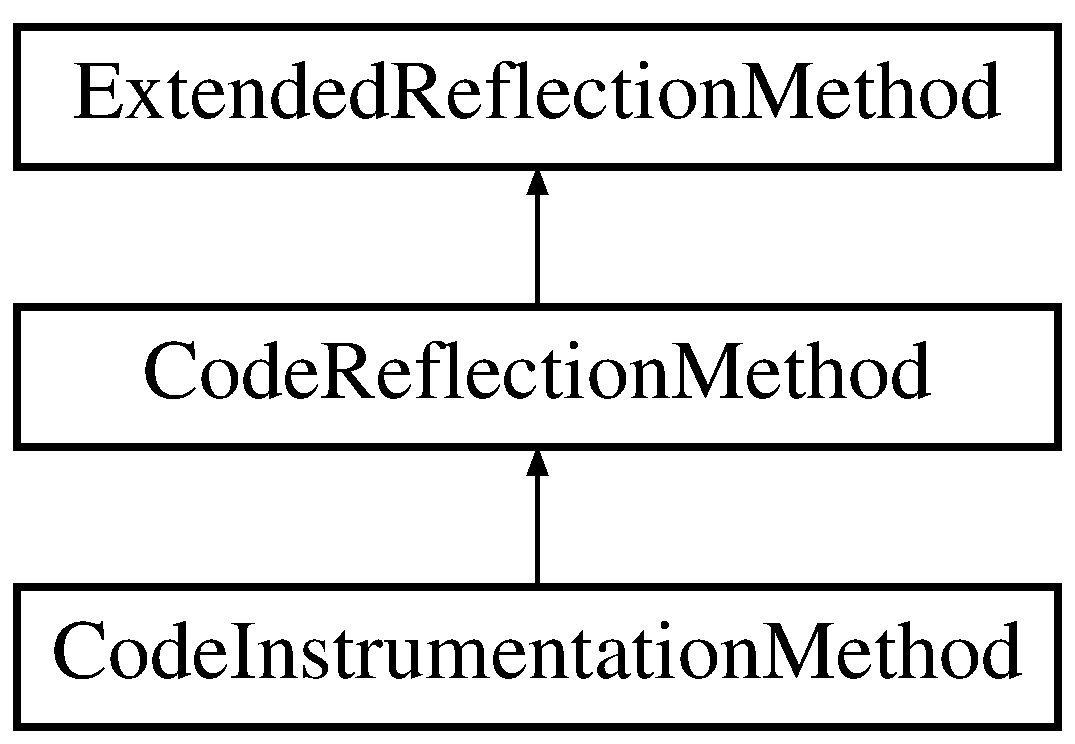
\includegraphics[height=3cm]{class_code_reflection_method}
\end{center}
\end{figure}
\subsection*{Public Member Functions}
\begin{CompactItemize}
\item 
\hyperlink{class_code_reflection_method_9ea590fa1500f62805d106332634893e}{getCode} ()
\item 
\hyperlink{class_code_reflection_method_49ef51345ba44d4a0c9242794f7a97a2}{getCodeContent} ()
\item 
\hyperlink{class_code_reflection_method_c4b3d9a1c136135c42a66302f52c66c5}{createMethodHeaderCode} ()
\end{CompactItemize}
\subsection*{Protected Member Functions}
\begin{CompactItemize}
\item 
\hyperlink{class_code_reflection_method_84c20b140478480a3bbecda5e9e13702}{createExtendedReflectionClass} (ReflectionClass \$objOriginalReflectionClass)
\item 
\hyperlink{class_code_reflection_method_33a3dcd4331a02b37addbc2fa9281af6}{createExtendedReflectionParameter} (ReflectionParameter \$objReflectionParameter)
\item 
\hyperlink{class_code_reflection_method_f2457c6e356d735b29253563175d0523}{createModifiersCode} ()
\item 
\hyperlink{class_code_reflection_method_803892b766bfd1aba81f5e63ed248676}{createParametersCode} ()
\item 
\hyperlink{class_code_reflection_method_4aa609e822a988c2577185932cad79eb}{createMethodContentCode} ()
\end{CompactItemize}


\subsection{Member Function Documentation}
\hypertarget{class_code_reflection_method_84c20b140478480a3bbecda5e9e13702}{
\index{CodeReflectionMethod@{CodeReflectionMethod}!createExtendedReflectionClass@{createExtendedReflectionClass}}
\index{createExtendedReflectionClass@{createExtendedReflectionClass}!CodeReflectionMethod@{CodeReflectionMethod}}
\subsubsection[{createExtendedReflectionClass}]{\setlength{\rightskip}{0pt plus 5cm}CodeReflectionMethod::createExtendedReflectionClass (ReflectionClass \$ {\em objOriginalReflectionClass})\hspace{0.3cm}{\tt  \mbox{[}protected\mbox{]}}}}
\label{class_code_reflection_method_84c20b140478480a3bbecda5e9e13702}


Create the link between the code reflection method and its code reflection class

\begin{Desc}
\item[See also:]ExtendedReflectionMethod::createExtendedReflectionClass( ReflectionClass ) \end{Desc}
\begin{Desc}
\item[Parameters:]
\begin{description}
\item[{\em ReflectionClass}]\$objOriginalReflectionClass \end{description}
\end{Desc}
\begin{Desc}
\item[Returns:]\hyperlink{class_code_reflection_class}{CodeReflectionClass} \end{Desc}


Reimplemented from \hyperlink{class_extended_reflection_method_e5727cf1a1b76d84e56a5fb312989ecb}{ExtendedReflectionMethod}.

Reimplemented in \hyperlink{class_code_instrumentation_method_7dda8c3f7ba312f14dd22d25a2b69ec1}{CodeInstrumentationMethod}.\hypertarget{class_code_reflection_method_33a3dcd4331a02b37addbc2fa9281af6}{
\index{CodeReflectionMethod@{CodeReflectionMethod}!createExtendedReflectionParameter@{createExtendedReflectionParameter}}
\index{createExtendedReflectionParameter@{createExtendedReflectionParameter}!CodeReflectionMethod@{CodeReflectionMethod}}
\subsubsection[{createExtendedReflectionParameter}]{\setlength{\rightskip}{0pt plus 5cm}CodeReflectionMethod::createExtendedReflectionParameter (ReflectionParameter \$ {\em objReflectionParameter})\hspace{0.3cm}{\tt  \mbox{[}protected\mbox{]}}}}
\label{class_code_reflection_method_33a3dcd4331a02b37addbc2fa9281af6}


Create the link between the code reflection method and its code reflection parameter

\begin{Desc}
\item[See also:]ExtendedReflectionMethod::createExtendedReflectionParameter( ReflectionParameter ) \end{Desc}
\begin{Desc}
\item[Parameters:]
\begin{description}
\item[{\em ReflectionParameter}]\$objReflectionParameter \end{description}
\end{Desc}
\begin{Desc}
\item[Returns:]\hyperlink{class_code_reflection_parameter}{CodeReflectionParameter} \end{Desc}


Reimplemented from \hyperlink{class_extended_reflection_method_a7d2760c2914c0ad6428171c4ca61503}{ExtendedReflectionMethod}.

Reimplemented in \hyperlink{class_code_instrumentation_method_d4a17b83d9e1fd997263bc1a9982ae3c}{CodeInstrumentationMethod}.\hypertarget{class_code_reflection_method_4aa609e822a988c2577185932cad79eb}{
\index{CodeReflectionMethod@{CodeReflectionMethod}!createMethodContentCode@{createMethodContentCode}}
\index{createMethodContentCode@{createMethodContentCode}!CodeReflectionMethod@{CodeReflectionMethod}}
\subsubsection[{createMethodContentCode}]{\setlength{\rightskip}{0pt plus 5cm}CodeReflectionMethod::createMethodContentCode ()\hspace{0.3cm}{\tt  \mbox{[}protected\mbox{]}}}}
\label{class_code_reflection_method_4aa609e822a988c2577185932cad79eb}


Create the method code definition content

\begin{Desc}
\item[Returns:]string \end{Desc}


Reimplemented in \hyperlink{class_code_instrumentation_method_731590867f98da76937a4e5a93ec2023}{CodeInstrumentationMethod}.\hypertarget{class_code_reflection_method_c4b3d9a1c136135c42a66302f52c66c5}{
\index{CodeReflectionMethod@{CodeReflectionMethod}!createMethodHeaderCode@{createMethodHeaderCode}}
\index{createMethodHeaderCode@{createMethodHeaderCode}!CodeReflectionMethod@{CodeReflectionMethod}}
\subsubsection[{createMethodHeaderCode}]{\setlength{\rightskip}{0pt plus 5cm}CodeReflectionMethod::createMethodHeaderCode ()}}
\label{class_code_reflection_method_c4b3d9a1c136135c42a66302f52c66c5}


Create the method code definition header

\begin{Desc}
\item[Returns:]string \end{Desc}


Reimplemented in \hyperlink{class_code_instrumentation_method_0eab7bf9706fa3867605f3db1822c333}{CodeInstrumentationMethod}.\hypertarget{class_code_reflection_method_f2457c6e356d735b29253563175d0523}{
\index{CodeReflectionMethod@{CodeReflectionMethod}!createModifiersCode@{createModifiersCode}}
\index{createModifiersCode@{createModifiersCode}!CodeReflectionMethod@{CodeReflectionMethod}}
\subsubsection[{createModifiersCode}]{\setlength{\rightskip}{0pt plus 5cm}CodeReflectionMethod::createModifiersCode ()\hspace{0.3cm}{\tt  \mbox{[}protected\mbox{]}}}}
\label{class_code_reflection_method_f2457c6e356d735b29253563175d0523}


Create the modifiers code definition of the method

\begin{Desc}
\item[Returns:]string \end{Desc}
\hypertarget{class_code_reflection_method_803892b766bfd1aba81f5e63ed248676}{
\index{CodeReflectionMethod@{CodeReflectionMethod}!createParametersCode@{createParametersCode}}
\index{createParametersCode@{createParametersCode}!CodeReflectionMethod@{CodeReflectionMethod}}
\subsubsection[{createParametersCode}]{\setlength{\rightskip}{0pt plus 5cm}CodeReflectionMethod::createParametersCode ()\hspace{0.3cm}{\tt  \mbox{[}protected\mbox{]}}}}
\label{class_code_reflection_method_803892b766bfd1aba81f5e63ed248676}


Create the parameters code definition

\begin{Desc}
\item[Returns:]string \end{Desc}
\hypertarget{class_code_reflection_method_9ea590fa1500f62805d106332634893e}{
\index{CodeReflectionMethod@{CodeReflectionMethod}!getCode@{getCode}}
\index{getCode@{getCode}!CodeReflectionMethod@{CodeReflectionMethod}}
\subsubsection[{getCode}]{\setlength{\rightskip}{0pt plus 5cm}CodeReflectionMethod::getCode ()}}
\label{class_code_reflection_method_9ea590fa1500f62805d106332634893e}


Create the code definition of the reflected method

\begin{Desc}
\item[Returns:]string code method definition \end{Desc}


Reimplemented in \hyperlink{class_code_instrumentation_method_b79054196e5abf3e3464ad0551a9af71}{CodeInstrumentationMethod}.\hypertarget{class_code_reflection_method_49ef51345ba44d4a0c9242794f7a97a2}{
\index{CodeReflectionMethod@{CodeReflectionMethod}!getCodeContent@{getCodeContent}}
\index{getCodeContent@{getCodeContent}!CodeReflectionMethod@{CodeReflectionMethod}}
\subsubsection[{getCodeContent}]{\setlength{\rightskip}{0pt plus 5cm}CodeReflectionMethod::getCodeContent ()}}
\label{class_code_reflection_method_49ef51345ba44d4a0c9242794f7a97a2}


Get the code content of the method

\begin{Desc}
\item[Returns:]string \end{Desc}


The documentation for this class was generated from the following file:\begin{CompactItemize}
\item 
components/codeReflection/\hyperlink{_code_reflection_method_8class_8php}{CodeReflectionMethod.class.php}\end{CompactItemize}

\hypertarget{class_code_reflection_parameter}{
\section{CodeReflectionParameter Class Reference}
\label{class_code_reflection_parameter}\index{CodeReflectionParameter@{CodeReflectionParameter}}
}
Inheritance diagram for CodeReflectionParameter::\begin{figure}[H]
\begin{center}
\leavevmode
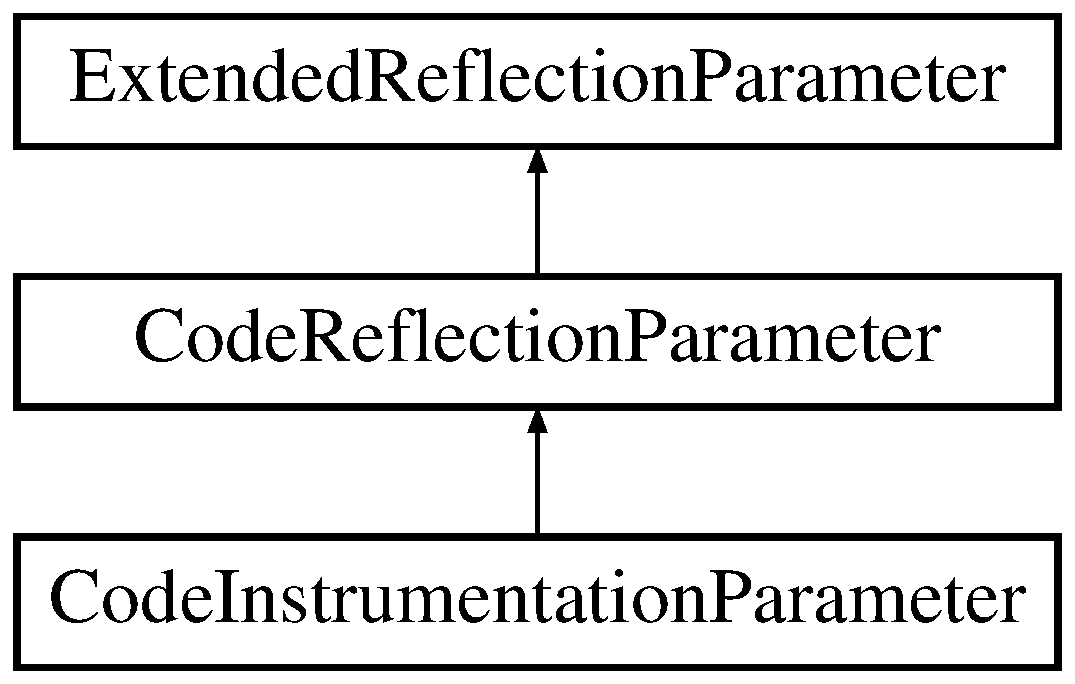
\includegraphics[height=3cm]{class_code_reflection_parameter}
\end{center}
\end{figure}
\subsection*{Public Member Functions}
\begin{CompactItemize}
\item 
\hyperlink{class_code_reflection_parameter_16918720d7f6522b9a9baa9cfbb4cfc7}{getCode} ()
\end{CompactItemize}
\subsection*{Protected Member Functions}
\begin{CompactItemize}
\item 
\hyperlink{class_code_reflection_parameter_a2b9b21f9711afbf11791dd64dcbdd0a}{createExtendedReflectionClass} (ReflectionClass \$objOriginalReflectionClass)
\item 
\hyperlink{class_code_reflection_parameter_04d7dbd71bc943f3e267869a79bec648}{createExtendedReflectionMethod} (ReflectionMethod \$objOriginalReflectionMethod)
\item 
\hyperlink{class_code_reflection_parameter_5e6e7a1f49ff1f404342a2b2d4a15aa3}{createExtendedReflectionFunction} (ReflectionFunction \$objOriginalReflectionFunction)
\end{CompactItemize}


\subsection{Member Function Documentation}
\hypertarget{class_code_reflection_parameter_a2b9b21f9711afbf11791dd64dcbdd0a}{
\index{CodeReflectionParameter@{CodeReflectionParameter}!createExtendedReflectionClass@{createExtendedReflectionClass}}
\index{createExtendedReflectionClass@{createExtendedReflectionClass}!CodeReflectionParameter@{CodeReflectionParameter}}
\subsubsection[{createExtendedReflectionClass}]{\setlength{\rightskip}{0pt plus 5cm}CodeReflectionParameter::createExtendedReflectionClass (ReflectionClass \$ {\em objOriginalReflectionClass})\hspace{0.3cm}{\tt  \mbox{[}protected\mbox{]}}}}
\label{class_code_reflection_parameter_a2b9b21f9711afbf11791dd64dcbdd0a}


Convert a reflection class into a extended reflection class

This is the method what should be replaced when this class be extended.

\begin{Desc}
\item[Parameters:]
\begin{description}
\item[{\em ReflectionClass}]\$objOriginalReflectionClass \end{description}
\end{Desc}
\begin{Desc}
\item[Returns:]\hyperlink{class_extended_reflection_class}{ExtendedReflectionClass} \end{Desc}


Reimplemented from \hyperlink{class_extended_reflection_parameter_7119682d1601c3398cbad195a4d52b4a}{ExtendedReflectionParameter}.

Reimplemented in \hyperlink{class_code_instrumentation_parameter_4190025f9ec55f58f10b36084a8851fd}{CodeInstrumentationParameter}.\hypertarget{class_code_reflection_parameter_5e6e7a1f49ff1f404342a2b2d4a15aa3}{
\index{CodeReflectionParameter@{CodeReflectionParameter}!createExtendedReflectionFunction@{createExtendedReflectionFunction}}
\index{createExtendedReflectionFunction@{createExtendedReflectionFunction}!CodeReflectionParameter@{CodeReflectionParameter}}
\subsubsection[{createExtendedReflectionFunction}]{\setlength{\rightskip}{0pt plus 5cm}CodeReflectionParameter::createExtendedReflectionFunction (ReflectionFunction \$ {\em objOriginalReflectionFunction})\hspace{0.3cm}{\tt  \mbox{[}protected\mbox{]}}}}
\label{class_code_reflection_parameter_5e6e7a1f49ff1f404342a2b2d4a15aa3}


Convert a reflection function into a extended reflection function

This is the method what should be replaced when this class be extended.

\begin{Desc}
\item[Parameters:]
\begin{description}
\item[{\em ReflectionFunction}]\$objOriginalReflectionFunction \end{description}
\end{Desc}
\begin{Desc}
\item[Returns:]\hyperlink{class_extended_reflection_function}{ExtendedReflectionFunction} \end{Desc}


Reimplemented from \hyperlink{class_extended_reflection_parameter_8bea4c5548f8e5476b28c37b705dc25e}{ExtendedReflectionParameter}.

Reimplemented in \hyperlink{class_code_instrumentation_parameter_e9723a389b48bdb31fc49f784692aecf}{CodeInstrumentationParameter}.\hypertarget{class_code_reflection_parameter_04d7dbd71bc943f3e267869a79bec648}{
\index{CodeReflectionParameter@{CodeReflectionParameter}!createExtendedReflectionMethod@{createExtendedReflectionMethod}}
\index{createExtendedReflectionMethod@{createExtendedReflectionMethod}!CodeReflectionParameter@{CodeReflectionParameter}}
\subsubsection[{createExtendedReflectionMethod}]{\setlength{\rightskip}{0pt plus 5cm}CodeReflectionParameter::createExtendedReflectionMethod (ReflectionMethod \$ {\em objOriginalReflectionMethod})\hspace{0.3cm}{\tt  \mbox{[}protected\mbox{]}}}}
\label{class_code_reflection_parameter_04d7dbd71bc943f3e267869a79bec648}


Convert a reflection method into a extended reflection method

This is the method what should be replaced when this class be extended.

\begin{Desc}
\item[Parameters:]
\begin{description}
\item[{\em ReflectionMethod}]\$objOriginalReflectionMethod \end{description}
\end{Desc}
\begin{Desc}
\item[Returns:]\hyperlink{class_extended_reflection_method}{ExtendedReflectionMethod} \end{Desc}


Reimplemented from \hyperlink{class_extended_reflection_parameter_fc7cab8ac6553754c4c4c62ba8be8685}{ExtendedReflectionParameter}.

Reimplemented in \hyperlink{class_code_instrumentation_parameter_e0c68e69aa93979e2e1fa3057bd39d5a}{CodeInstrumentationParameter}.\hypertarget{class_code_reflection_parameter_16918720d7f6522b9a9baa9cfbb4cfc7}{
\index{CodeReflectionParameter@{CodeReflectionParameter}!getCode@{getCode}}
\index{getCode@{getCode}!CodeReflectionParameter@{CodeReflectionParameter}}
\subsubsection[{getCode}]{\setlength{\rightskip}{0pt plus 5cm}CodeReflectionParameter::getCode ()}}
\label{class_code_reflection_parameter_16918720d7f6522b9a9baa9cfbb4cfc7}


Get the code from the parameter

\begin{Desc}
\item[Returns:]String \end{Desc}


\href{http://bugs.php.net/bug.php?id=33312}{\tt http://bugs.php.net/bug.php?id=33312}

The documentation for this class was generated from the following file:\begin{CompactItemize}
\item 
components/codeReflection/\hyperlink{_code_reflection_parameter_8class_8php}{CodeReflectionParameter.class.php}\end{CompactItemize}

\hypertarget{class_code_reflection_property}{
\section{CodeReflectionProperty Class Reference}
\label{class_code_reflection_property}\index{CodeReflectionProperty@{CodeReflectionProperty}}
}
Inheritance diagram for CodeReflectionProperty::\begin{figure}[H]
\begin{center}
\leavevmode
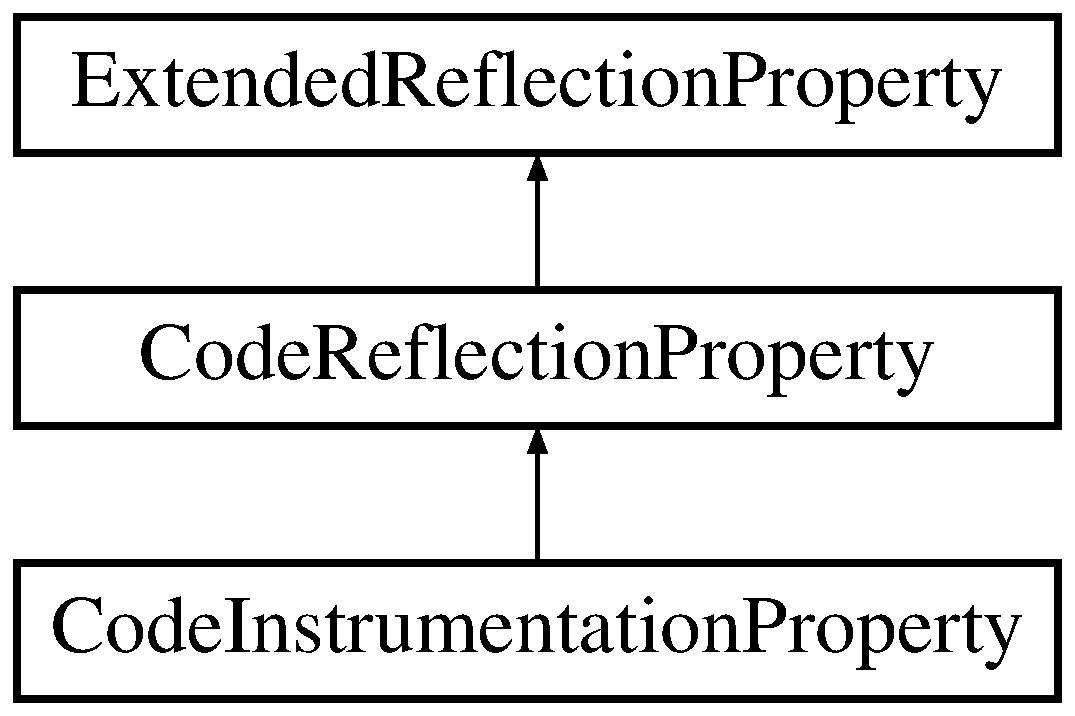
\includegraphics[height=3cm]{class_code_reflection_property}
\end{center}
\end{figure}
\subsection*{Public Member Functions}
\begin{CompactItemize}
\item 
\hyperlink{class_code_reflection_property_f9b9401c63918169457fe8516324950f}{getDefaultValue} ()
\item 
\hyperlink{class_code_reflection_property_b5e24da53b4a0d0848b18c1e832f47ff}{getCode} ()
\end{CompactItemize}
\subsection*{Protected Member Functions}
\begin{CompactItemize}
\item 
\hyperlink{class_code_reflection_property_6b56ec198bc6a5b5a72076e4e7c19e29}{createExtendedReflectionClass} (ReflectionClass \$objOriginalReflectionClass)
\end{CompactItemize}


\subsection{Detailed Description}
Code Reflection Property it is a code reflection version of the reflection property

\begin{Desc}
\item[Author:]Thiago Henrique Ramos da Mata $<$\href{mailto:thiago.henrique.mata@gmail.com}{\tt thiago.henrique.mata@gmail.com}$>$ \end{Desc}


\subsection{Member Function Documentation}
\hypertarget{class_code_reflection_property_6b56ec198bc6a5b5a72076e4e7c19e29}{
\index{CodeReflectionProperty@{CodeReflectionProperty}!createExtendedReflectionClass@{createExtendedReflectionClass}}
\index{createExtendedReflectionClass@{createExtendedReflectionClass}!CodeReflectionProperty@{CodeReflectionProperty}}
\subsubsection[{createExtendedReflectionClass}]{\setlength{\rightskip}{0pt plus 5cm}createExtendedReflectionClass (ReflectionClass \$ {\em objOriginalReflectionClass})\hspace{0.3cm}{\tt  \mbox{[}protected\mbox{]}}}}
\label{class_code_reflection_property_6b56ec198bc6a5b5a72076e4e7c19e29}


Convert a reflection class into a extended reflection class

This is the method what should be replaced when this class be extended.

\begin{Desc}
\item[Parameters:]
\begin{description}
\item[{\em ReflectionClass}]\$objOriginalReflectionClass \end{description}
\end{Desc}
\begin{Desc}
\item[Returns:]\hyperlink{class_extended_reflection_class}{ExtendedReflectionClass} \end{Desc}


Reimplemented from \hyperlink{class_extended_reflection_property_6b56ec198bc6a5b5a72076e4e7c19e29}{ExtendedReflectionProperty}.

Reimplemented in \hyperlink{class_code_instrumentation_property_6b56ec198bc6a5b5a72076e4e7c19e29}{CodeInstrumentationProperty}.

\begin{Code}\begin{verbatim}84         {
85                 return new CodeReflectionClass( $objOriginalReflectionClass->getName() );
86         }
\end{verbatim}
\end{Code}


\hypertarget{class_code_reflection_property_b5e24da53b4a0d0848b18c1e832f47ff}{
\index{CodeReflectionProperty@{CodeReflectionProperty}!getCode@{getCode}}
\index{getCode@{getCode}!CodeReflectionProperty@{CodeReflectionProperty}}
\subsubsection[{getCode}]{\setlength{\rightskip}{0pt plus 5cm}getCode ()}}
\label{class_code_reflection_property_b5e24da53b4a0d0848b18c1e832f47ff}




\begin{Code}\begin{verbatim}55         {
56 
57         $strCode = "";
58                 $strCode .= CorujaStringManipulation::retab( $this->getDocComment() , 1 );
59                 if( $this->isPrivate() )
60                 {
61                         $strCode .= " private ";
62                 }
63                 if( $this->isProtected())
64                 {
65                         $strCode .= " protected ";
66                 }
67                 if( $this->isPublic())
68                 {
69                         $strCode .= " public ";
70                 }
71                 if( $this->isStatic() )
72                 {
73                         $strCode .= " static ";
74                 }
75                 $strCode .= '$'. $this->getName();
76 
77         $strCode .= ' = ' . var_export( $this->getDefaultValue() , true );
78                 $strCode .= ";" . "\n";
79 
80                 return $strCode;
81         }
\end{verbatim}
\end{Code}


\hypertarget{class_code_reflection_property_f9b9401c63918169457fe8516324950f}{
\index{CodeReflectionProperty@{CodeReflectionProperty}!getDefaultValue@{getDefaultValue}}
\index{getDefaultValue@{getDefaultValue}!CodeReflectionProperty@{CodeReflectionProperty}}
\subsubsection[{getDefaultValue}]{\setlength{\rightskip}{0pt plus 5cm}getDefaultValue ()}}
\label{class_code_reflection_property_f9b9401c63918169457fe8516324950f}


Get the default value of the property.

While the PHP Reflection don't make this method native. We have to create this workaround to get the default value of the attribute. This brings a problem of classes what need of paramenters into it's constructors. In this cases, the default value will be ignored.

getDafaultValue don't exist into reflection  unable to get default value on constructors with parameters \begin{Desc}
\item[\hyperlink{todo__todo000003}{Todo}]get the default value of the attribute reading direct from the file \end{Desc}
\begin{Desc}
\item[Returns:]mix \end{Desc}


\begin{Code}\begin{verbatim}30     {
31         /*
32         try
33         {
34             $objParent = $this->getDeclaringClass();
35             $strClassName = $objParent->getClassName();
36             $objTemp = new $strClassName();
37             $arrTemp = (array)$objTemp;
38             $arrNew = array();
39             foreach( $arrTemp as $strKeyTemp => $mixValue )
40             {
41                 $strNewKey = substr( $strKeyTemp , 3 );
42                 $arrNew[ $strNewKey ] = $mixValue;
43             }
44             return $arrNew[ $this->getName() ];
45         }catch( Exception $objException )
46         {
47             // error on init object //
48             return null;
49         }
50          * *
51          */
52         return null;
53     }
\end{verbatim}
\end{Code}




The documentation for this class was generated from the following file:\begin{CompactItemize}
\item 
components/codeReflection/\hyperlink{_code_reflection_property_8class_8php}{CodeReflectionProperty.class.php}\end{CompactItemize}

\hypertarget{class_code_to_diagram_exception}{
\section{CodeToDiagramException Class Reference}
\label{class_code_to_diagram_exception}\index{CodeToDiagramException@{CodeToDiagramException}}
}


\subsection{Detailed Description}
Code To Diagram Exception

\begin{Desc}
\item[Author:]Thiago Henrique Ramos da Mata $<$\href{mailto:thiago.henrique.mata@gmail.com}{\tt thiago.henrique.mata@gmail.com}$>$ \end{Desc}


The documentation for this class was generated from the following file:\begin{CompactItemize}
\item 
components/codeToDiagram/\hyperlink{_code_to_diagram_exception_8class_8php}{CodeToDiagramException.class.php}\end{CompactItemize}

\hypertarget{class_coruja_array_manipulation_test}{
\section{CorujaArrayManipulationTest Class Reference}
\label{class_coruja_array_manipulation_test}\index{CorujaArrayManipulationTest@{CorujaArrayManipulationTest}}
}
\subsection*{Public Member Functions}
\begin{CompactItemize}
\item 
\hyperlink{class_coruja_array_manipulation_test_78b308f298161af48c3887029536a731}{testGetArrayFieldWithNullArray} ()
\item 
\hyperlink{class_coruja_array_manipulation_test_8399ad4b91876142e2d69ba6077c04eb}{testGetArrayFieldWithNoKey} ()
\item 
\hyperlink{class_coruja_array_manipulation_test_48ada181c4be1fc27b5b5542599ac884}{testGetArrayFieldWithNoneArray} ()
\item 
\hyperlink{class_coruja_array_manipulation_test_2b39098a7334b209f5e54877bf165e9b}{testGetArrayFieldWithExistingKey} ()
\item 
\hyperlink{class_coruja_array_manipulation_test_f87353adad0450eaa29c202a0b132262}{testGetArrayFieldWithNoneExistingKey} ()
\item 
\hyperlink{class_coruja_array_manipulation_test_9e14aea717bc3184296db73c59340944}{testGetArrayFieldWithNoneExistingKeyAndThirdParameter} ()
\item 
\hyperlink{class_coruja_array_manipulation_test_ea02b7a01e6a9cd620b4848be8559b7a}{testGetArrayFieldWithNullKey} ()
\end{CompactItemize}
\subsection*{Protected Member Functions}
\begin{CompactItemize}
\item 
\hyperlink{class_coruja_array_manipulation_test_0bc688732d2b3b162ffebaf7812e78da}{setUp} ()
\item 
\hyperlink{class_coruja_array_manipulation_test_80fe3d17e658907fc75346a0ec9d6fc7}{tearDown} ()
\end{CompactItemize}


\subsection{Detailed Description}
Test class for \hyperlink{class_coruja_array_manipulation}{CorujaArrayManipulation}. Generated by PHPUnit on 2008-10-24 at 21:41:40. 

\subsection{Member Function Documentation}
\hypertarget{class_coruja_array_manipulation_test_0bc688732d2b3b162ffebaf7812e78da}{
\index{CorujaArrayManipulationTest@{CorujaArrayManipulationTest}!setUp@{setUp}}
\index{setUp@{setUp}!CorujaArrayManipulationTest@{CorujaArrayManipulationTest}}
\subsubsection[{setUp}]{\setlength{\rightskip}{0pt plus 5cm}setUp ()\hspace{0.3cm}{\tt  \mbox{[}protected\mbox{]}}}}
\label{class_coruja_array_manipulation_test_0bc688732d2b3b162ffebaf7812e78da}


Sets up the fixture, for example, opens a network connection. This method is called before a test is executed.

protected 

\begin{Code}\begin{verbatim}19     {
20     }
\end{verbatim}
\end{Code}


\hypertarget{class_coruja_array_manipulation_test_80fe3d17e658907fc75346a0ec9d6fc7}{
\index{CorujaArrayManipulationTest@{CorujaArrayManipulationTest}!tearDown@{tearDown}}
\index{tearDown@{tearDown}!CorujaArrayManipulationTest@{CorujaArrayManipulationTest}}
\subsubsection[{tearDown}]{\setlength{\rightskip}{0pt plus 5cm}tearDown ()\hspace{0.3cm}{\tt  \mbox{[}protected\mbox{]}}}}
\label{class_coruja_array_manipulation_test_80fe3d17e658907fc75346a0ec9d6fc7}


Tears down the fixture, for example, closes a network connection. This method is called after a test is executed.

protected 

\begin{Code}\begin{verbatim}29     {
30     }
\end{verbatim}
\end{Code}


\hypertarget{class_coruja_array_manipulation_test_2b39098a7334b209f5e54877bf165e9b}{
\index{CorujaArrayManipulationTest@{CorujaArrayManipulationTest}!testGetArrayFieldWithExistingKey@{testGetArrayFieldWithExistingKey}}
\index{testGetArrayFieldWithExistingKey@{testGetArrayFieldWithExistingKey}!CorujaArrayManipulationTest@{CorujaArrayManipulationTest}}
\subsubsection[{testGetArrayFieldWithExistingKey}]{\setlength{\rightskip}{0pt plus 5cm}testGetArrayFieldWithExistingKey ()}}
\label{class_coruja_array_manipulation_test_2b39098a7334b209f5e54877bf165e9b}




\begin{Code}\begin{verbatim}90                                                        {
91 
92         // set up
93         $array = array("one");
94 
95         // exercise
96         $fieldValue = CorujaArrayManipulation::getArrayField( $array, 0 );
97 
98         // assert
99         $this->assertEquals( "one", $fieldValue );
100     }
\end{verbatim}
\end{Code}


\hypertarget{class_coruja_array_manipulation_test_8399ad4b91876142e2d69ba6077c04eb}{
\index{CorujaArrayManipulationTest@{CorujaArrayManipulationTest}!testGetArrayFieldWithNoKey@{testGetArrayFieldWithNoKey}}
\index{testGetArrayFieldWithNoKey@{testGetArrayFieldWithNoKey}!CorujaArrayManipulationTest@{CorujaArrayManipulationTest}}
\subsubsection[{testGetArrayFieldWithNoKey}]{\setlength{\rightskip}{0pt plus 5cm}testGetArrayFieldWithNoKey ()}}
\label{class_coruja_array_manipulation_test_8399ad4b91876142e2d69ba6077c04eb}


\begin{Desc}
\item[\hyperlink{todo__todo000004}{Todo}]Implement testGetArrayField(). \end{Desc}


\begin{Code}\begin{verbatim}50                                                  {
51 
52         // set up
53         $array = array("one");
54 
55         // exercise
56         $fieldValue = CorujaArrayManipulation::getArrayField( $array );
57 
58         // assert
59 
60 
61         // Remove the following lines when you implement this test.
62         $this->markTestIncomplete(
63           'Behavior not defined yet.'
64         );
65     }
\end{verbatim}
\end{Code}


\hypertarget{class_coruja_array_manipulation_test_48ada181c4be1fc27b5b5542599ac884}{
\index{CorujaArrayManipulationTest@{CorujaArrayManipulationTest}!testGetArrayFieldWithNoneArray@{testGetArrayFieldWithNoneArray}}
\index{testGetArrayFieldWithNoneArray@{testGetArrayFieldWithNoneArray}!CorujaArrayManipulationTest@{CorujaArrayManipulationTest}}
\subsubsection[{testGetArrayFieldWithNoneArray}]{\setlength{\rightskip}{0pt plus 5cm}testGetArrayFieldWithNoneArray ()}}
\label{class_coruja_array_manipulation_test_48ada181c4be1fc27b5b5542599ac884}


\begin{Desc}
\item[\hyperlink{todo__todo000005}{Todo}]Implement testGetArrayField(). \end{Desc}


\begin{Code}\begin{verbatim}70                                                      {
71 
72         // set up
73         $integer = 2;
74 
75         // exercise
76         $fieldValue = CorujaArrayManipulation::getArrayField( $integer, 0 );
77 
78         // assert
79 
80 
81         // Remove the following lines when you implement this test.
82         $this->markTestIncomplete(
83           'Behavior not defined yet.'
84         );
85     }
\end{verbatim}
\end{Code}


\hypertarget{class_coruja_array_manipulation_test_f87353adad0450eaa29c202a0b132262}{
\index{CorujaArrayManipulationTest@{CorujaArrayManipulationTest}!testGetArrayFieldWithNoneExistingKey@{testGetArrayFieldWithNoneExistingKey}}
\index{testGetArrayFieldWithNoneExistingKey@{testGetArrayFieldWithNoneExistingKey}!CorujaArrayManipulationTest@{CorujaArrayManipulationTest}}
\subsubsection[{testGetArrayFieldWithNoneExistingKey}]{\setlength{\rightskip}{0pt plus 5cm}testGetArrayFieldWithNoneExistingKey ()}}
\label{class_coruja_array_manipulation_test_f87353adad0450eaa29c202a0b132262}




\begin{Code}\begin{verbatim}105                                                            {
106 
107         // set up
108         $array = array("one");
109 
110         // exercise
111         $fieldValue = CorujaArrayManipulation::getArrayField( $array, 2 );
112 
113         // assert
114         $this->assertNull( $fieldValue );
115     }
\end{verbatim}
\end{Code}


\hypertarget{class_coruja_array_manipulation_test_9e14aea717bc3184296db73c59340944}{
\index{CorujaArrayManipulationTest@{CorujaArrayManipulationTest}!testGetArrayFieldWithNoneExistingKeyAndThirdParameter@{testGetArrayFieldWithNoneExistingKeyAndThirdParameter}}
\index{testGetArrayFieldWithNoneExistingKeyAndThirdParameter@{testGetArrayFieldWithNoneExistingKeyAndThirdParameter}!CorujaArrayManipulationTest@{CorujaArrayManipulationTest}}
\subsubsection[{testGetArrayFieldWithNoneExistingKeyAndThirdParameter}]{\setlength{\rightskip}{0pt plus 5cm}testGetArrayFieldWithNoneExistingKeyAndThirdParameter ()}}
\label{class_coruja_array_manipulation_test_9e14aea717bc3184296db73c59340944}




\begin{Code}\begin{verbatim}120                                                                             {
121 
122         // set up
123         $array = array("one");
124 
125         // exercise
126         $fieldValue = CorujaArrayManipulation::getArrayField( $array, 2, "anything" );
127 
128         // assert
129         $this->assertEquals( "anything", $fieldValue );
130     }
\end{verbatim}
\end{Code}


\hypertarget{class_coruja_array_manipulation_test_78b308f298161af48c3887029536a731}{
\index{CorujaArrayManipulationTest@{CorujaArrayManipulationTest}!testGetArrayFieldWithNullArray@{testGetArrayFieldWithNullArray}}
\index{testGetArrayFieldWithNullArray@{testGetArrayFieldWithNullArray}!CorujaArrayManipulationTest@{CorujaArrayManipulationTest}}
\subsubsection[{testGetArrayFieldWithNullArray}]{\setlength{\rightskip}{0pt plus 5cm}testGetArrayFieldWithNullArray ()}}
\label{class_coruja_array_manipulation_test_78b308f298161af48c3887029536a731}




\begin{Code}\begin{verbatim}35                                                      {
36 
37         // set up
38         $array = null;
39 
40         // exercise
41         $fieldValue = CorujaArrayManipulation::getArrayField( $array );
42 
43         // assert
44         $this->assertNull( $fieldValue );
45     }
\end{verbatim}
\end{Code}


\hypertarget{class_coruja_array_manipulation_test_ea02b7a01e6a9cd620b4848be8559b7a}{
\index{CorujaArrayManipulationTest@{CorujaArrayManipulationTest}!testGetArrayFieldWithNullKey@{testGetArrayFieldWithNullKey}}
\index{testGetArrayFieldWithNullKey@{testGetArrayFieldWithNullKey}!CorujaArrayManipulationTest@{CorujaArrayManipulationTest}}
\subsubsection[{testGetArrayFieldWithNullKey}]{\setlength{\rightskip}{0pt plus 5cm}testGetArrayFieldWithNullKey ()}}
\label{class_coruja_array_manipulation_test_ea02b7a01e6a9cd620b4848be8559b7a}




\begin{Code}\begin{verbatim}135                                                    {
136 
137         // set up
138         $array = array("one");
139 
140         // exercise
141         $fieldValue = CorujaArrayManipulation::getArrayField( $array, null, "anything" );
142 
143         // assert
144         $this->assertEquals( "anything", $fieldValue );
145     }
\end{verbatim}
\end{Code}




The documentation for this class was generated from the following file:\begin{CompactItemize}
\item 
components/library/test/\hyperlink{_coruja_array_manipulation_test_8php}{CorujaArrayManipulationTest.php}\end{CompactItemize}

\hypertarget{class_coruja_class_manipulation_test}{
\section{CorujaClassManipulationTest Class Reference}
\label{class_coruja_class_manipulation_test}\index{CorujaClassManipulationTest@{CorujaClassManipulationTest}}
}
\subsection*{Public Member Functions}
\begin{CompactItemize}
\item 
\hyperlink{class_coruja_class_manipulation_test_597f3fd79250591e51a07532b84520fa}{testGetClassNameFromClassDefinitionWithNullString} ()
\item 
\hyperlink{class_coruja_class_manipulation_test_ff7a03d9aea2786f8cb04b38b194b53f}{testGetClassNameFromClassDefinitionWithAnyString} ()
\item 
\hyperlink{class_coruja_class_manipulation_test_922c39d49268128861fac863098fb660}{testGetClassNameFromClassDefinitionWithNormalClassDefinition} ()
\item 
\hyperlink{class_coruja_class_manipulation_test_ce9cf206ad48a158cd897305919b68cf}{testGetNamespaceFromClassDefinitionWithNullString} ()
\item 
\hyperlink{class_coruja_class_manipulation_test_53d2c075bd350927691fcd7171e6cf44}{testGetNamespaceFromClassDefinitionWithAnyString} ()
\item 
\hyperlink{class_coruja_class_manipulation_test_4bc6c516b02ff2e92a533a1ed066ccbf}{testGetNamespaceFromClassDefinitionWithNormalClassDefinition} ()
\end{CompactItemize}
\subsection*{Protected Member Functions}
\begin{CompactItemize}
\item 
\hyperlink{class_coruja_class_manipulation_test_0689ef78070e399d14d8152d797ad32f}{setUp} ()
\item 
\hyperlink{class_coruja_class_manipulation_test_bb345ca2d0b9f7c3525edbc0f3ace254}{tearDown} ()
\end{CompactItemize}


\subsection{Detailed Description}
Test class for CorujaClassManipulation. Generated by PHPUnit on 2008-10-24 at 22:47:23. 

\subsection{Member Function Documentation}
\hypertarget{class_coruja_class_manipulation_test_0689ef78070e399d14d8152d797ad32f}{
\index{CorujaClassManipulationTest@{CorujaClassManipulationTest}!setUp@{setUp}}
\index{setUp@{setUp}!CorujaClassManipulationTest@{CorujaClassManipulationTest}}
\subsubsection[{setUp}]{\setlength{\rightskip}{0pt plus 5cm}CorujaClassManipulationTest::setUp ()\hspace{0.3cm}{\tt  \mbox{[}protected\mbox{]}}}}
\label{class_coruja_class_manipulation_test_0689ef78070e399d14d8152d797ad32f}


Sets up the fixture, for example, opens a network connection. This method is called before a test is executed.

protected \hypertarget{class_coruja_class_manipulation_test_bb345ca2d0b9f7c3525edbc0f3ace254}{
\index{CorujaClassManipulationTest@{CorujaClassManipulationTest}!tearDown@{tearDown}}
\index{tearDown@{tearDown}!CorujaClassManipulationTest@{CorujaClassManipulationTest}}
\subsubsection[{tearDown}]{\setlength{\rightskip}{0pt plus 5cm}CorujaClassManipulationTest::tearDown ()\hspace{0.3cm}{\tt  \mbox{[}protected\mbox{]}}}}
\label{class_coruja_class_manipulation_test_bb345ca2d0b9f7c3525edbc0f3ace254}


Tears down the fixture, for example, closes a network connection. This method is called after a test is executed.

protected \hypertarget{class_coruja_class_manipulation_test_ff7a03d9aea2786f8cb04b38b194b53f}{
\index{CorujaClassManipulationTest@{CorujaClassManipulationTest}!testGetClassNameFromClassDefinitionWithAnyString@{testGetClassNameFromClassDefinitionWithAnyString}}
\index{testGetClassNameFromClassDefinitionWithAnyString@{testGetClassNameFromClassDefinitionWithAnyString}!CorujaClassManipulationTest@{CorujaClassManipulationTest}}
\subsubsection[{testGetClassNameFromClassDefinitionWithAnyString}]{\setlength{\rightskip}{0pt plus 5cm}CorujaClassManipulationTest::testGetClassNameFromClassDefinitionWithAnyString ()}}
\label{class_coruja_class_manipulation_test_ff7a03d9aea2786f8cb04b38b194b53f}


\begin{Desc}
\item[\hyperlink{todo__todo000007}{Todo}]Implement testGetClassNameFromClassDefintion(). \end{Desc}
\hypertarget{class_coruja_class_manipulation_test_922c39d49268128861fac863098fb660}{
\index{CorujaClassManipulationTest@{CorujaClassManipulationTest}!testGetClassNameFromClassDefinitionWithNormalClassDefinition@{testGetClassNameFromClassDefinitionWithNormalClassDefinition}}
\index{testGetClassNameFromClassDefinitionWithNormalClassDefinition@{testGetClassNameFromClassDefinitionWithNormalClassDefinition}!CorujaClassManipulationTest@{CorujaClassManipulationTest}}
\subsubsection[{testGetClassNameFromClassDefinitionWithNormalClassDefinition}]{\setlength{\rightskip}{0pt plus 5cm}CorujaClassManipulationTest::testGetClassNameFromClassDefinitionWithNormalClassDefinition ()}}
\label{class_coruja_class_manipulation_test_922c39d49268128861fac863098fb660}


\hypertarget{class_coruja_class_manipulation_test_597f3fd79250591e51a07532b84520fa}{
\index{CorujaClassManipulationTest@{CorujaClassManipulationTest}!testGetClassNameFromClassDefinitionWithNullString@{testGetClassNameFromClassDefinitionWithNullString}}
\index{testGetClassNameFromClassDefinitionWithNullString@{testGetClassNameFromClassDefinitionWithNullString}!CorujaClassManipulationTest@{CorujaClassManipulationTest}}
\subsubsection[{testGetClassNameFromClassDefinitionWithNullString}]{\setlength{\rightskip}{0pt plus 5cm}CorujaClassManipulationTest::testGetClassNameFromClassDefinitionWithNullString ()}}
\label{class_coruja_class_manipulation_test_597f3fd79250591e51a07532b84520fa}


\begin{Desc}
\item[\hyperlink{todo__todo000006}{Todo}]Implement testGetClassNameFromClassDefintion(). \end{Desc}
\hypertarget{class_coruja_class_manipulation_test_53d2c075bd350927691fcd7171e6cf44}{
\index{CorujaClassManipulationTest@{CorujaClassManipulationTest}!testGetNamespaceFromClassDefinitionWithAnyString@{testGetNamespaceFromClassDefinitionWithAnyString}}
\index{testGetNamespaceFromClassDefinitionWithAnyString@{testGetNamespaceFromClassDefinitionWithAnyString}!CorujaClassManipulationTest@{CorujaClassManipulationTest}}
\subsubsection[{testGetNamespaceFromClassDefinitionWithAnyString}]{\setlength{\rightskip}{0pt plus 5cm}CorujaClassManipulationTest::testGetNamespaceFromClassDefinitionWithAnyString ()}}
\label{class_coruja_class_manipulation_test_53d2c075bd350927691fcd7171e6cf44}


\begin{Desc}
\item[\hyperlink{todo__todo000009}{Todo}]Implement testGetNamespaceFromClassDefinition(). \end{Desc}
\hypertarget{class_coruja_class_manipulation_test_4bc6c516b02ff2e92a533a1ed066ccbf}{
\index{CorujaClassManipulationTest@{CorujaClassManipulationTest}!testGetNamespaceFromClassDefinitionWithNormalClassDefinition@{testGetNamespaceFromClassDefinitionWithNormalClassDefinition}}
\index{testGetNamespaceFromClassDefinitionWithNormalClassDefinition@{testGetNamespaceFromClassDefinitionWithNormalClassDefinition}!CorujaClassManipulationTest@{CorujaClassManipulationTest}}
\subsubsection[{testGetNamespaceFromClassDefinitionWithNormalClassDefinition}]{\setlength{\rightskip}{0pt plus 5cm}CorujaClassManipulationTest::testGetNamespaceFromClassDefinitionWithNormalClassDefinition ()}}
\label{class_coruja_class_manipulation_test_4bc6c516b02ff2e92a533a1ed066ccbf}


\hypertarget{class_coruja_class_manipulation_test_ce9cf206ad48a158cd897305919b68cf}{
\index{CorujaClassManipulationTest@{CorujaClassManipulationTest}!testGetNamespaceFromClassDefinitionWithNullString@{testGetNamespaceFromClassDefinitionWithNullString}}
\index{testGetNamespaceFromClassDefinitionWithNullString@{testGetNamespaceFromClassDefinitionWithNullString}!CorujaClassManipulationTest@{CorujaClassManipulationTest}}
\subsubsection[{testGetNamespaceFromClassDefinitionWithNullString}]{\setlength{\rightskip}{0pt plus 5cm}CorujaClassManipulationTest::testGetNamespaceFromClassDefinitionWithNullString ()}}
\label{class_coruja_class_manipulation_test_ce9cf206ad48a158cd897305919b68cf}


\begin{Desc}
\item[\hyperlink{todo__todo000008}{Todo}]Implement testGetNamespaceFromClassDefinition(). \end{Desc}


The documentation for this class was generated from the following file:\begin{CompactItemize}
\item 
components/library/test/\hyperlink{_coruja_class_manipulation_test_8php}{CorujaClassManipulationTest.php}\end{CompactItemize}

\hypertarget{class_example_code_reflecion}{
\section{ExampleCodeReflecion Class Reference}
\label{class_example_code_reflecion}\index{ExampleCodeReflecion@{ExampleCodeReflecion}}
}
Inheritance diagram for ExampleCodeReflecion::\begin{figure}[H]
\begin{center}
\leavevmode
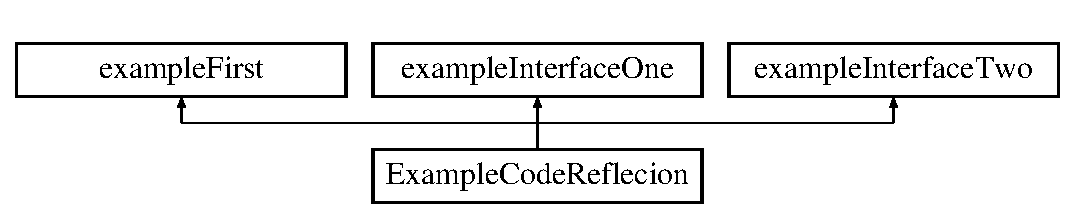
\includegraphics[height=2cm]{class_example_code_reflecion}
\end{center}
\end{figure}
\subsection*{Public Member Functions}
\begin{CompactItemize}
\item 
\hyperlink{class_example_code_reflecion_bf19f7a457cf5f0e92ecd5f42e76018e}{doSomethingCool} (\$strName=\char`\"{}hi\char`\"{}, exampleSecond \$obSecond=null, \hyperlink{classexample_second}{exampleSecond} \$objLastOne=null)
\item 
\hyperlink{class_example_code_reflecion_7d29a36398226ef64512719c29c01a0f}{hardWork} ()
\end{CompactItemize}
\subsection*{Static Protected Attributes}
\begin{CompactItemize}
\item 
static \hyperlink{class_example_code_reflecion_b1f249f4c625c843e88d641a6a71199a}{\$arrParadas} = array()
\end{CompactItemize}
\subsection*{Static Private Member Functions}
\begin{CompactItemize}
\item 
static \hyperlink{class_example_code_reflecion_82081362ac40db52076731b35d8aa5f4}{doNothing} ()
\end{CompactItemize}
\subsection*{Private Attributes}
\begin{CompactItemize}
\item 
\hyperlink{class_example_code_reflecion_90edf7538a74be8ac5ce46baaf203382}{\$strName}
\end{CompactItemize}


\subsection{Member Function Documentation}
\hypertarget{class_example_code_reflecion_82081362ac40db52076731b35d8aa5f4}{
\index{ExampleCodeReflecion@{ExampleCodeReflecion}!doNothing@{doNothing}}
\index{doNothing@{doNothing}!ExampleCodeReflecion@{ExampleCodeReflecion}}
\subsubsection[{doNothing}]{\setlength{\rightskip}{0pt plus 5cm}static doNothing ()\hspace{0.3cm}{\tt  \mbox{[}static, private\mbox{]}}}}
\label{class_example_code_reflecion_82081362ac40db52076731b35d8aa5f4}




\begin{Code}\begin{verbatim}39         {
40                 // empty...
41         }
\end{verbatim}
\end{Code}


\hypertarget{class_example_code_reflecion_bf19f7a457cf5f0e92ecd5f42e76018e}{
\index{ExampleCodeReflecion@{ExampleCodeReflecion}!doSomethingCool@{doSomethingCool}}
\index{doSomethingCool@{doSomethingCool}!ExampleCodeReflecion@{ExampleCodeReflecion}}
\subsubsection[{doSomethingCool}]{\setlength{\rightskip}{0pt plus 5cm}doSomethingCool (\$ {\em strName} = {\tt \char`\"{}hi\char`\"{}}, \/  {\bf exampleSecond} \$ {\em obSecond} = {\tt null}, \/  {\bf exampleSecond} \$ {\em objLastOne} = {\tt null})\hspace{0.3cm}{\tt  \mbox{[}final\mbox{]}}}}
\label{class_example_code_reflecion_bf19f7a457cf5f0e92ecd5f42e76018e}


Will do something cool

\begin{Desc}
\item[Returns:]string \end{Desc}


\begin{Code}\begin{verbatim}32         {
33                 $this->strName = $strName;
34                 print "i change the name to " . $this->strName;
35                 $this->doNothing();
36         }
\end{verbatim}
\end{Code}


\hypertarget{class_example_code_reflecion_7d29a36398226ef64512719c29c01a0f}{
\index{ExampleCodeReflecion@{ExampleCodeReflecion}!hardWork@{hardWork}}
\index{hardWork@{hardWork}!ExampleCodeReflecion@{ExampleCodeReflecion}}
\subsubsection[{hardWork}]{\setlength{\rightskip}{0pt plus 5cm}hardWork ()}}
\label{class_example_code_reflecion_7d29a36398226ef64512719c29c01a0f}




\begin{Code}\begin{verbatim}44         {
45                 for( $i = 0 ; $i < 20 ; $i++ )
46                 {
47                         $this->doSomethingCool( $i );
48                 }
49         }
\end{verbatim}
\end{Code}




\subsection{Member Data Documentation}
\hypertarget{class_example_code_reflecion_b1f249f4c625c843e88d641a6a71199a}{
\index{ExampleCodeReflecion@{ExampleCodeReflecion}!\$arrParadas@{\$arrParadas}}
\index{\$arrParadas@{\$arrParadas}!ExampleCodeReflecion@{ExampleCodeReflecion}}
\subsubsection[{\$arrParadas}]{\setlength{\rightskip}{0pt plus 5cm}\$arrParadas = array()\hspace{0.3cm}{\tt  \mbox{[}static, protected\mbox{]}}}}
\label{class_example_code_reflecion_b1f249f4c625c843e88d641a6a71199a}


\hypertarget{class_example_code_reflecion_90edf7538a74be8ac5ce46baaf203382}{
\index{ExampleCodeReflecion@{ExampleCodeReflecion}!\$strName@{\$strName}}
\index{\$strName@{\$strName}!ExampleCodeReflecion@{ExampleCodeReflecion}}
\subsubsection[{\$strName}]{\setlength{\rightskip}{0pt plus 5cm}\$strName\hspace{0.3cm}{\tt  \mbox{[}private\mbox{]}}}}
\label{class_example_code_reflecion_90edf7538a74be8ac5ce46baaf203382}


else

string 

The documentation for this class was generated from the following file:\begin{CompactItemize}
\item 
components/codeReflection/example/\hyperlink{code_reflection_2example_2test1_8php}{test1.php}\end{CompactItemize}

\hypertarget{classexample_first}{
\section{exampleFirst Class Reference}
\label{classexample_first}\index{exampleFirst@{exampleFirst}}
}
Inheritance diagram for exampleFirst::\begin{figure}[H]
\begin{center}
\leavevmode
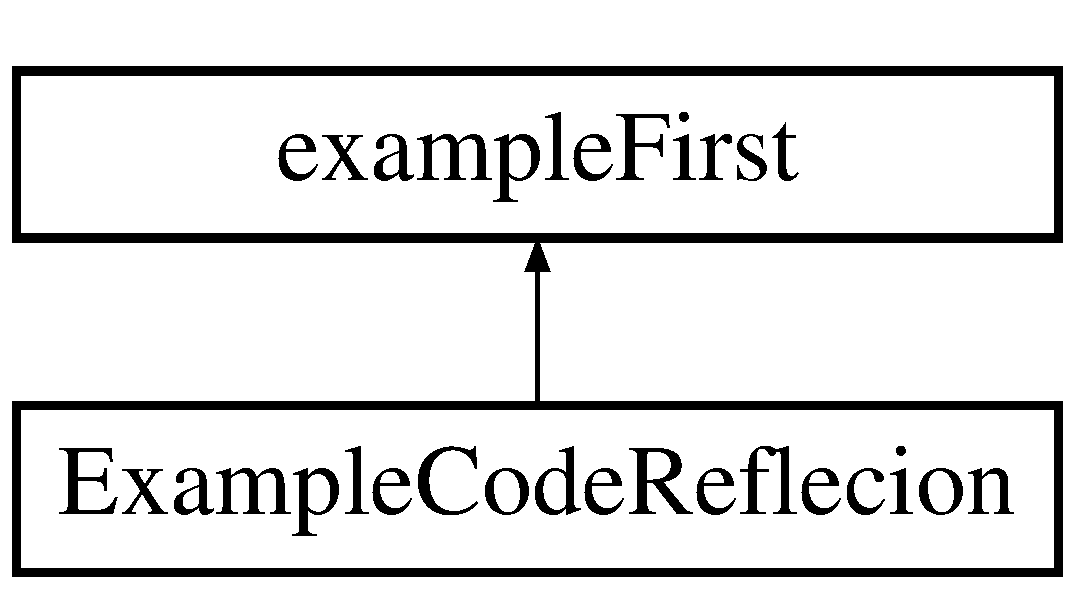
\includegraphics[height=2cm]{classexample_first}
\end{center}
\end{figure}


\subsection{Detailed Description}
This example will consist into change the content of some methods using the debug reflection and namespaces. 

The documentation for this class was generated from the following file:\begin{CompactItemize}
\item 
components/codeReflection/example/\hyperlink{code_reflection_2example_2test1_8php}{test1.php}\end{CompactItemize}

\hypertarget{interfaceexample_interface_one}{
\section{exampleInterfaceOne Interface Reference}
\label{interfaceexample_interface_one}\index{exampleInterfaceOne@{exampleInterfaceOne}}
}
Inheritance diagram for exampleInterfaceOne::\begin{figure}[H]
\begin{center}
\leavevmode
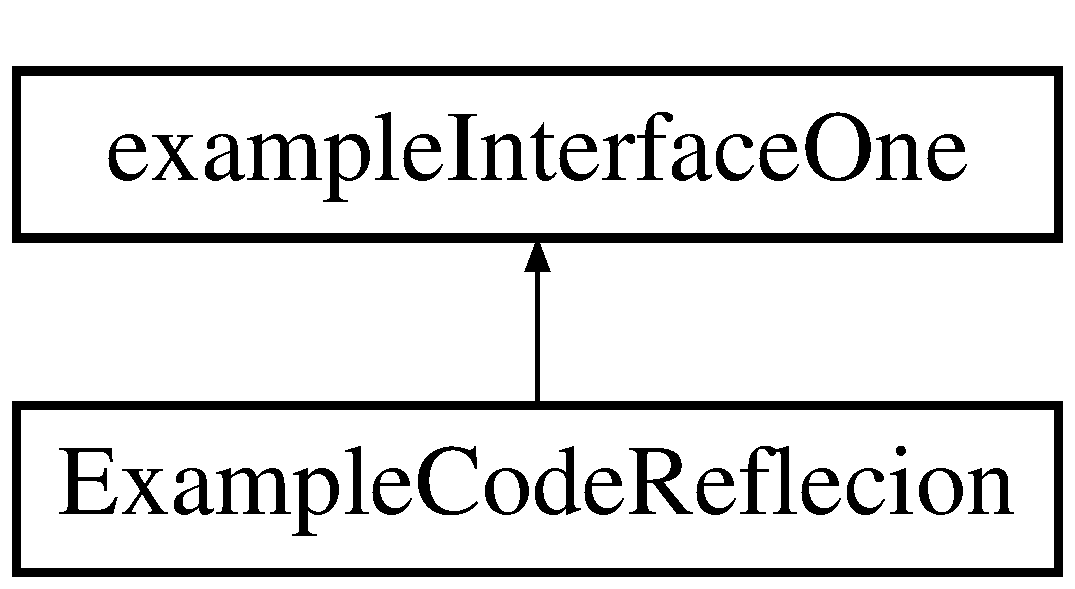
\includegraphics[height=2cm]{interfaceexample_interface_one}
\end{center}
\end{figure}


The documentation for this interface was generated from the following file:\begin{CompactItemize}
\item 
components/codeReflection/example/\hyperlink{code_reflection_2example_2test1_8php}{test1.php}\end{CompactItemize}

\hypertarget{interfaceexample_interface_two}{
\section{exampleInterfaceTwo Interface Reference}
\label{interfaceexample_interface_two}\index{exampleInterfaceTwo@{exampleInterfaceTwo}}
}
Inheritance diagram for exampleInterfaceTwo::\begin{figure}[H]
\begin{center}
\leavevmode
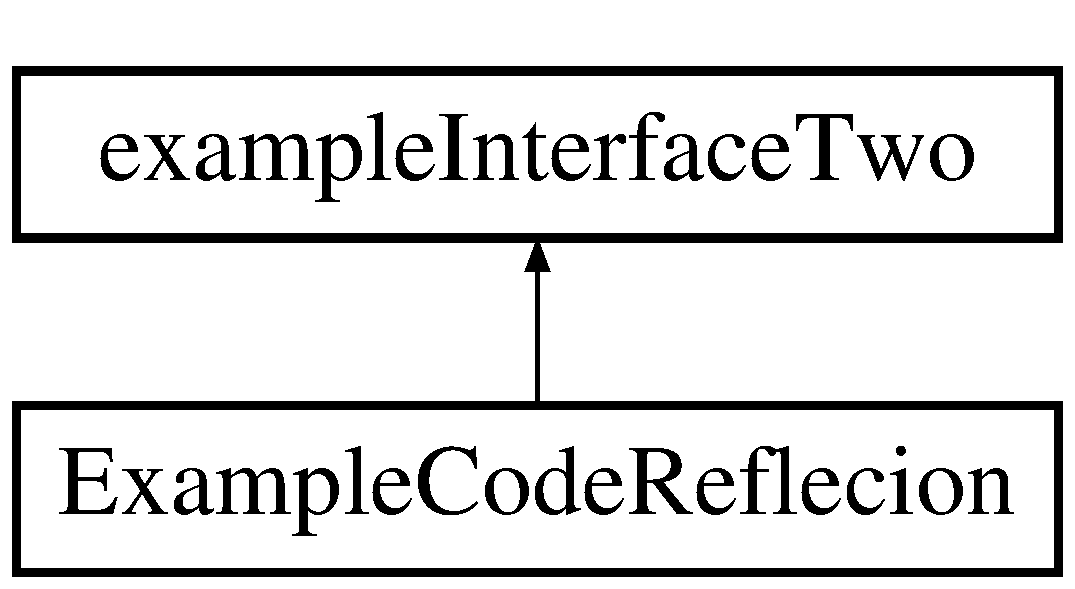
\includegraphics[height=2cm]{interfaceexample_interface_two}
\end{center}
\end{figure}


The documentation for this interface was generated from the following file:\begin{CompactItemize}
\item 
components/codeReflection/example/\hyperlink{code_reflection_2example_2test1_8php}{test1.php}\end{CompactItemize}

\hypertarget{classexample_second}{
\section{exampleSecond Class Reference}
\label{classexample_second}\index{exampleSecond@{exampleSecond}}
}


The documentation for this class was generated from the following file:\begin{CompactItemize}
\item 
components/codeReflection/example/\hyperlink{code_reflection_2example_2test1_8php}{test1.php}\end{CompactItemize}

\hypertarget{class_extended_reflection_class}{
\section{ExtendedReflectionClass Class Reference}
\label{class_extended_reflection_class}\index{ExtendedReflectionClass@{ExtendedReflectionClass}}
}
Inheritance diagram for ExtendedReflectionClass::\begin{figure}[H]
\begin{center}
\leavevmode
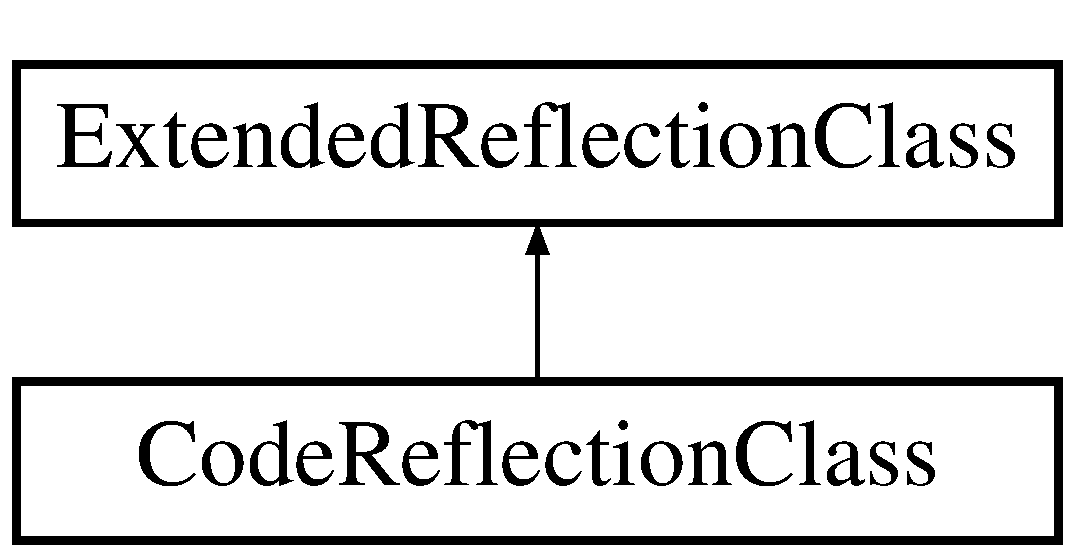
\includegraphics[height=2cm]{class_extended_reflection_class}
\end{center}
\end{figure}
\subsection*{Public Member Functions}
\begin{CompactItemize}
\item 
\hyperlink{class_extended_reflection_class_dbce950becc27c205b461ff9c61aaec2}{getParentClass} ()
\item 
\hyperlink{class_extended_reflection_class_bd1fa7af7876ada7e09c2d4727201b45}{getInterfaces} ()
\item 
\hyperlink{class_extended_reflection_class_8f6bf6f713d03f9ffedf453e65155eab}{getProperties} (\$filter=-1)
\item 
\hyperlink{class_extended_reflection_class_5c58929a1f0a44664ba38d4c05d1cd47}{getProperty} (\$strName)
\item 
\hyperlink{class_extended_reflection_class_01f8e033ec5d82ae20394345fcb06841}{getMethods} (\$filter=-1)
\item 
\hyperlink{class_extended_reflection_class_87cabc3e5bca9750380f3c06cc613d0a}{getMethod} (\$strMethodName)
\end{CompactItemize}
\subsection*{Protected Member Functions}
\begin{CompactItemize}
\item 
\hyperlink{class_extended_reflection_class_851f69035820c89d0ba918a277d2a29f}{createExtendedReflectionClass} (ReflectionClass \$objOriginalReflectionClass)
\item 
\hyperlink{class_extended_reflection_class_6259683f3d0f9583ec36ca51f6e964f9}{createExtendedReflectionProperty} (ReflectionProperty \$objOriginalReflectionProperty)
\item 
\hyperlink{class_extended_reflection_class_922598bd80a21577ccad6d4ca4138474}{createExtendedReflectionMethod} (ReflectionMethod \$objOriginalReflectionMethod)
\end{CompactItemize}


\subsection{Member Function Documentation}
\hypertarget{class_extended_reflection_class_851f69035820c89d0ba918a277d2a29f}{
\index{ExtendedReflectionClass@{ExtendedReflectionClass}!createExtendedReflectionClass@{createExtendedReflectionClass}}
\index{createExtendedReflectionClass@{createExtendedReflectionClass}!ExtendedReflectionClass@{ExtendedReflectionClass}}
\subsubsection[{createExtendedReflectionClass}]{\setlength{\rightskip}{0pt plus 5cm}ExtendedReflectionClass::createExtendedReflectionClass (ReflectionClass \$ {\em objOriginalReflectionClass})\hspace{0.3cm}{\tt  \mbox{[}protected\mbox{]}}}}
\label{class_extended_reflection_class_851f69035820c89d0ba918a277d2a29f}


Convert a reflection class into a extended reflection class

This is the method what should be replaced when this class be extended.

\begin{Desc}
\item[Parameters:]
\begin{description}
\item[{\em ReflectionClass}]\$objOriginalReflectionClass \end{description}
\end{Desc}
\begin{Desc}
\item[Returns:]\hyperlink{class_extended_reflection_class}{ExtendedReflectionClass} \end{Desc}


Reimplemented in \hyperlink{class_code_reflection_class_496631cb5814727379cdacb689e4c40a}{CodeReflectionClass}.\hypertarget{class_extended_reflection_class_922598bd80a21577ccad6d4ca4138474}{
\index{ExtendedReflectionClass@{ExtendedReflectionClass}!createExtendedReflectionMethod@{createExtendedReflectionMethod}}
\index{createExtendedReflectionMethod@{createExtendedReflectionMethod}!ExtendedReflectionClass@{ExtendedReflectionClass}}
\subsubsection[{createExtendedReflectionMethod}]{\setlength{\rightskip}{0pt plus 5cm}ExtendedReflectionClass::createExtendedReflectionMethod (ReflectionMethod \$ {\em objOriginalReflectionMethod})\hspace{0.3cm}{\tt  \mbox{[}protected\mbox{]}}}}
\label{class_extended_reflection_class_922598bd80a21577ccad6d4ca4138474}


Convert a reflection method into a extended reflection method

This is the method what should be replaced when this class be extended.

\begin{Desc}
\item[Parameters:]
\begin{description}
\item[{\em ReflectionMethod}]\$objOriginalReflectionMethod \end{description}
\end{Desc}
\begin{Desc}
\item[Returns:]\hyperlink{class_extended_reflection_method}{ExtendedReflectionMethod} \end{Desc}


Reimplemented in \hyperlink{class_code_reflection_class_c8e58a7369660bf8f63ce39f3b9b5271}{CodeReflectionClass}.\hypertarget{class_extended_reflection_class_6259683f3d0f9583ec36ca51f6e964f9}{
\index{ExtendedReflectionClass@{ExtendedReflectionClass}!createExtendedReflectionProperty@{createExtendedReflectionProperty}}
\index{createExtendedReflectionProperty@{createExtendedReflectionProperty}!ExtendedReflectionClass@{ExtendedReflectionClass}}
\subsubsection[{createExtendedReflectionProperty}]{\setlength{\rightskip}{0pt plus 5cm}ExtendedReflectionClass::createExtendedReflectionProperty (ReflectionProperty \$ {\em objOriginalReflectionProperty})\hspace{0.3cm}{\tt  \mbox{[}protected\mbox{]}}}}
\label{class_extended_reflection_class_6259683f3d0f9583ec36ca51f6e964f9}


Convert a reflection property into a extended reflection property

This is the method what should be replaced when this class be extended.

\begin{Desc}
\item[Parameters:]
\begin{description}
\item[{\em ReflectionProperty}]\$objOriginalReflectionProperty \end{description}
\end{Desc}
\begin{Desc}
\item[Returns:]\hyperlink{class_extended_reflection_property}{ExtendedReflectionProperty} \end{Desc}


Reimplemented in \hyperlink{class_code_reflection_class_838dcd22317018c53f02dda69cd07509}{CodeReflectionClass}.\hypertarget{class_extended_reflection_class_bd1fa7af7876ada7e09c2d4727201b45}{
\index{ExtendedReflectionClass@{ExtendedReflectionClass}!getInterfaces@{getInterfaces}}
\index{getInterfaces@{getInterfaces}!ExtendedReflectionClass@{ExtendedReflectionClass}}
\subsubsection[{getInterfaces}]{\setlength{\rightskip}{0pt plus 5cm}ExtendedReflectionClass::getInterfaces ()\hspace{0.3cm}{\tt  \mbox{[}final\mbox{]}}}}
\label{class_extended_reflection_class_bd1fa7af7876ada7e09c2d4727201b45}


Get the collection of the reflection class of all the interfaces implemented by the reflected class

\begin{Desc}
\item[Returns:]\hyperlink{class_extended_reflection_class}{ExtendedReflectionClass}\mbox{[}\mbox{]} \end{Desc}
\hypertarget{class_extended_reflection_class_87cabc3e5bca9750380f3c06cc613d0a}{
\index{ExtendedReflectionClass@{ExtendedReflectionClass}!getMethod@{getMethod}}
\index{getMethod@{getMethod}!ExtendedReflectionClass@{ExtendedReflectionClass}}
\subsubsection[{getMethod}]{\setlength{\rightskip}{0pt plus 5cm}ExtendedReflectionClass::getMethod (\$ {\em strMethodName})\hspace{0.3cm}{\tt  \mbox{[}final\mbox{]}}}}
\label{class_extended_reflection_class_87cabc3e5bca9750380f3c06cc613d0a}


Return the reflection of some method of the class

\begin{Desc}
\item[Parameters:]
\begin{description}
\item[{\em \$strMethodName}]\end{description}
\end{Desc}
\begin{Desc}
\item[Returns:]\hyperlink{class_extended_reflection_method}{ExtendedReflectionMethod} \end{Desc}
\hypertarget{class_extended_reflection_class_01f8e033ec5d82ae20394345fcb06841}{
\index{ExtendedReflectionClass@{ExtendedReflectionClass}!getMethods@{getMethods}}
\index{getMethods@{getMethods}!ExtendedReflectionClass@{ExtendedReflectionClass}}
\subsubsection[{getMethods}]{\setlength{\rightskip}{0pt plus 5cm}ExtendedReflectionClass::getMethods (\$ {\em filter} = {\tt -1})\hspace{0.3cm}{\tt  \mbox{[}final\mbox{]}}}}
\label{class_extended_reflection_class_01f8e033ec5d82ae20394345fcb06841}


Get the collection of the reflected methods

\begin{Desc}
\item[Parameters:]
\begin{description}
\item[{\em \$filter}]\end{description}
\end{Desc}
\begin{Desc}
\item[Returns:]ReflectionMethod\mbox{[}\mbox{]} \end{Desc}
\hypertarget{class_extended_reflection_class_dbce950becc27c205b461ff9c61aaec2}{
\index{ExtendedReflectionClass@{ExtendedReflectionClass}!getParentClass@{getParentClass}}
\index{getParentClass@{getParentClass}!ExtendedReflectionClass@{ExtendedReflectionClass}}
\subsubsection[{getParentClass}]{\setlength{\rightskip}{0pt plus 5cm}ExtendedReflectionClass::getParentClass ()\hspace{0.3cm}{\tt  \mbox{[}final\mbox{]}}}}
\label{class_extended_reflection_class_dbce950becc27c205b461ff9c61aaec2}


Get the reflection of the parent class if extists and return null if not has a parent class

\begin{Desc}
\item[Returns:]ExtendedReflectionClass$|$null \end{Desc}
\hypertarget{class_extended_reflection_class_8f6bf6f713d03f9ffedf453e65155eab}{
\index{ExtendedReflectionClass@{ExtendedReflectionClass}!getProperties@{getProperties}}
\index{getProperties@{getProperties}!ExtendedReflectionClass@{ExtendedReflectionClass}}
\subsubsection[{getProperties}]{\setlength{\rightskip}{0pt plus 5cm}ExtendedReflectionClass::getProperties (\$ {\em filter} = {\tt -1})\hspace{0.3cm}{\tt  \mbox{[}final\mbox{]}}}}
\label{class_extended_reflection_class_8f6bf6f713d03f9ffedf453e65155eab}


Get the collection of the reflection properties of the reflected class

\begin{Desc}
\item[Parameters:]
\begin{description}
\item[{\em integer}]\$filter \end{description}
\end{Desc}
\begin{Desc}
\item[Returns:]ReflectionProperty\mbox{[}\mbox{]} \end{Desc}
\hypertarget{class_extended_reflection_class_5c58929a1f0a44664ba38d4c05d1cd47}{
\index{ExtendedReflectionClass@{ExtendedReflectionClass}!getProperty@{getProperty}}
\index{getProperty@{getProperty}!ExtendedReflectionClass@{ExtendedReflectionClass}}
\subsubsection[{getProperty}]{\setlength{\rightskip}{0pt plus 5cm}ExtendedReflectionClass::getProperty (\$ {\em strName})\hspace{0.3cm}{\tt  \mbox{[}final\mbox{]}}}}
\label{class_extended_reflection_class_5c58929a1f0a44664ba38d4c05d1cd47}


Get the reflection property of some attribute of the class searched by the property name

\begin{Desc}
\item[Parameters:]
\begin{description}
\item[{\em string}]\$strName \end{description}
\end{Desc}
\begin{Desc}
\item[Returns:]\hyperlink{class_extended_reflection_property}{ExtendedReflectionProperty} \end{Desc}


The documentation for this class was generated from the following file:\begin{CompactItemize}
\item 
components/extendedReflection/\hyperlink{_extended_reflection_class_8class_8php}{ExtendedReflectionClass.class.php}\end{CompactItemize}

\hypertarget{class_extended_reflection_function}{
\section{ExtendedReflectionFunction Class Reference}
\label{class_extended_reflection_function}\index{ExtendedReflectionFunction@{ExtendedReflectionFunction}}
}
Inheritance diagram for ExtendedReflectionFunction::\begin{figure}[H]
\begin{center}
\leavevmode
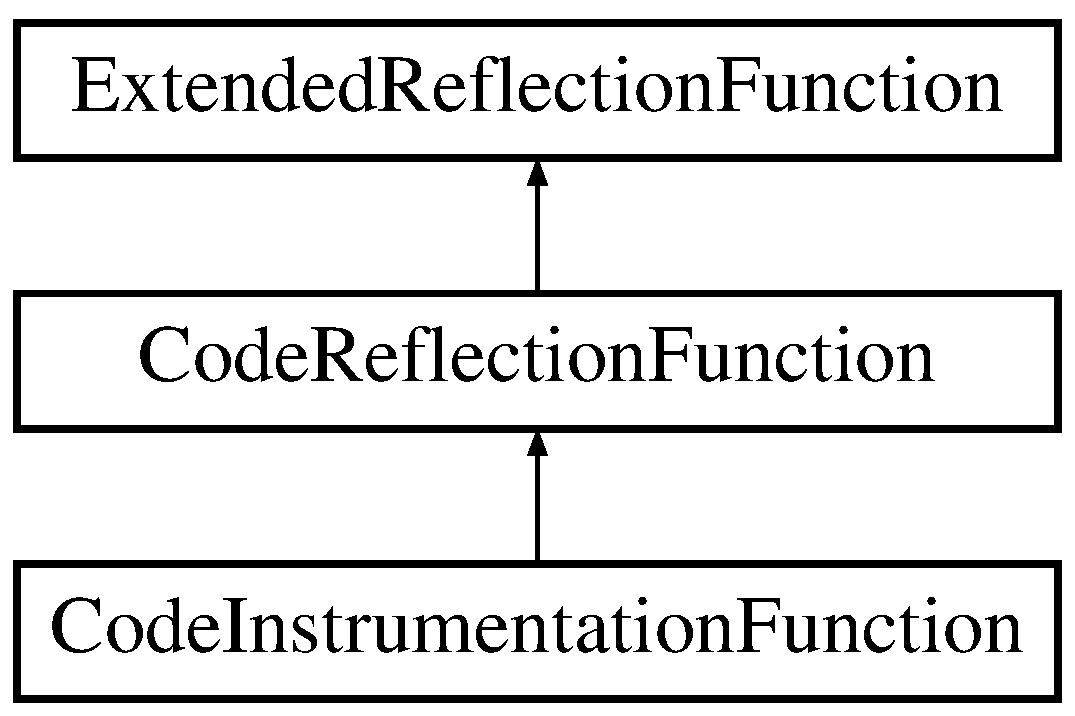
\includegraphics[height=3cm]{class_extended_reflection_function}
\end{center}
\end{figure}
\subsection*{Public Member Functions}
\begin{CompactItemize}
\item 
\hyperlink{class_extended_reflection_function_015cb52e5774a1972d296c9694d2a3c3}{getParameters} ()
\end{CompactItemize}
\subsection*{Protected Member Functions}
\begin{CompactItemize}
\item 
\hyperlink{class_extended_reflection_function_98ceb248f2b535a3a83ac2e7990e0c1f}{createExtendedReflectionParameter} (ReflectionParameter \$objReflectionParameter)
\end{CompactItemize}


\subsection{Detailed Description}
Class what make possible and easy extend reflection function

Reflection classes can be a problem because the reflection methods what return objects will return the original reflection object and not the extended version of it. So it is necessary to create methods what convert the original methods to return the extended version of the objects.

\begin{Desc}
\item[Author:]Thiago Henrique Ramos da Mata $<$\href{mailto:thiago.henrique.mata@gmail.com}{\tt thiago.henrique.mata@gmail.com}$>$ \end{Desc}


\subsection{Member Function Documentation}
\hypertarget{class_extended_reflection_function_98ceb248f2b535a3a83ac2e7990e0c1f}{
\index{ExtendedReflectionFunction@{ExtendedReflectionFunction}!createExtendedReflectionParameter@{createExtendedReflectionParameter}}
\index{createExtendedReflectionParameter@{createExtendedReflectionParameter}!ExtendedReflectionFunction@{ExtendedReflectionFunction}}
\subsubsection[{createExtendedReflectionParameter}]{\setlength{\rightskip}{0pt plus 5cm}createExtendedReflectionParameter (ReflectionParameter \$ {\em objReflectionParameter})\hspace{0.3cm}{\tt  \mbox{[}protected\mbox{]}}}}
\label{class_extended_reflection_function_98ceb248f2b535a3a83ac2e7990e0c1f}


Convert a reflection parameter into a extended reflection parameter

This is the method what should be replaced when this class be extended.

\begin{Desc}
\item[Parameters:]
\begin{description}
\item[{\em ReflectionParameter}]\$objReflectionParameter \end{description}
\end{Desc}
\begin{Desc}
\item[Returns:]\hyperlink{class_extended_reflection_parameter}{ExtendedReflectionParameter} \end{Desc}


Reimplemented in \hyperlink{class_code_instrumentation_function_98ceb248f2b535a3a83ac2e7990e0c1f}{CodeInstrumentationFunction}, and \hyperlink{class_code_reflection_function_98ceb248f2b535a3a83ac2e7990e0c1f}{CodeReflectionFunction}.

\begin{Code}\begin{verbatim}48         {
49                 return new ExtendedReflectionParameter( $this->getDeclaringClass()->getName() , $this->getName() , $objReflectionParameter->getName() );
50         }
\end{verbatim}
\end{Code}


\hypertarget{class_extended_reflection_function_015cb52e5774a1972d296c9694d2a3c3}{
\index{ExtendedReflectionFunction@{ExtendedReflectionFunction}!getParameters@{getParameters}}
\index{getParameters@{getParameters}!ExtendedReflectionFunction@{ExtendedReflectionFunction}}
\subsubsection[{getParameters}]{\setlength{\rightskip}{0pt plus 5cm}getParameters ()\hspace{0.3cm}{\tt  \mbox{[}final\mbox{]}}}}
\label{class_extended_reflection_function_015cb52e5774a1972d296c9694d2a3c3}


Return a list of the parameters of the reflected function

\begin{Desc}
\item[Returns:]\hyperlink{class_extended_reflection_parameter}{ExtendedReflectionParameter}\mbox{[}\mbox{]} \end{Desc}


\begin{Code}\begin{verbatim}27     {
28         $arrReflectionParameters = parent::getParameters();
29         $arrExtendedParameters = array();
30                 foreach( $arrReflectionParameters as $objReflectionParameter )
31                 {
32                         /*@var $objReflectionParameter ReflectionParameter */
33                         $arrExtendedParameteres[] = $this->createExtendedReflectionParameter( $objReflectionParameter );
34                 }
35                 return $arrExtendedParameters;
36     }
\end{verbatim}
\end{Code}




The documentation for this class was generated from the following file:\begin{CompactItemize}
\item 
components/extendedReflection/\hyperlink{_extended_reflection_function_8class_8php}{ExtendedReflectionFunction.class.php}\end{CompactItemize}

\hypertarget{class_extended_reflection_method}{
\section{ExtendedReflectionMethod Class Reference}
\label{class_extended_reflection_method}\index{ExtendedReflectionMethod@{ExtendedReflectionMethod}}
}
Inheritance diagram for ExtendedReflectionMethod::\begin{figure}[H]
\begin{center}
\leavevmode
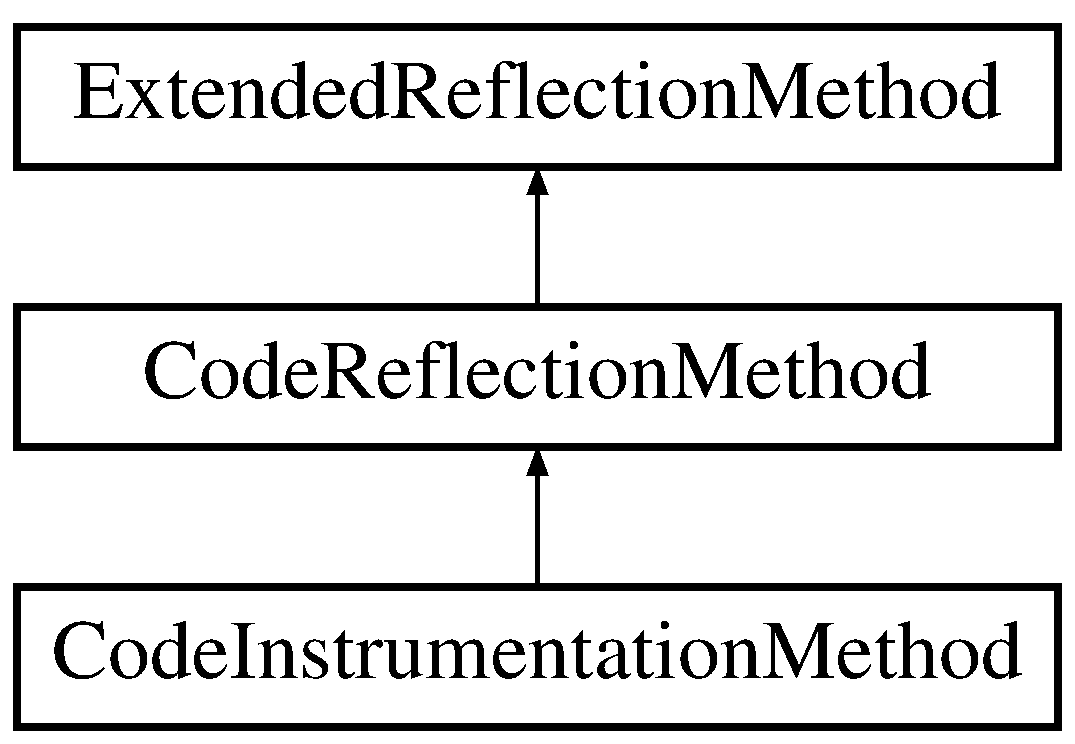
\includegraphics[height=3cm]{class_extended_reflection_method}
\end{center}
\end{figure}
\subsection*{Public Member Functions}
\begin{CompactItemize}
\item 
\hyperlink{class_extended_reflection_method_acff3f8d93cc250281f0f73bff3422e1}{getDeclaringClass} ()
\item 
\hyperlink{class_extended_reflection_method_015cb52e5774a1972d296c9694d2a3c3}{getParameters} ()
\end{CompactItemize}
\subsection*{Protected Member Functions}
\begin{CompactItemize}
\item 
\hyperlink{class_extended_reflection_method_6b56ec198bc6a5b5a72076e4e7c19e29}{createExtendedReflectionClass} (ReflectionClass \$objOriginalReflectionClass)
\item 
\hyperlink{class_extended_reflection_method_98ceb248f2b535a3a83ac2e7990e0c1f}{createExtendedReflectionParameter} (ReflectionParameter \$objReflectionParameter)
\end{CompactItemize}


\subsection{Detailed Description}
Class what make possible and easy extend reflection method

Reflection classes can be a problem because the reflection methods what return objects will return the original reflection object and not the extended version of it. So it is necessary to create methods what convert the original methods to return the extended version of the objects.

\begin{Desc}
\item[Author:]Thiago Henrique Ramos da Mata $<$\href{mailto:thiago.henrique.mata@gmail.com}{\tt thiago.henrique.mata@gmail.com}$>$ \end{Desc}


\subsection{Member Function Documentation}
\hypertarget{class_extended_reflection_method_6b56ec198bc6a5b5a72076e4e7c19e29}{
\index{ExtendedReflectionMethod@{ExtendedReflectionMethod}!createExtendedReflectionClass@{createExtendedReflectionClass}}
\index{createExtendedReflectionClass@{createExtendedReflectionClass}!ExtendedReflectionMethod@{ExtendedReflectionMethod}}
\subsubsection[{createExtendedReflectionClass}]{\setlength{\rightskip}{0pt plus 5cm}createExtendedReflectionClass (ReflectionClass \$ {\em objOriginalReflectionClass})\hspace{0.3cm}{\tt  \mbox{[}protected\mbox{]}}}}
\label{class_extended_reflection_method_6b56ec198bc6a5b5a72076e4e7c19e29}


Convert a reflection class into a extended reflection class

This is the method what should be replaced when this class be extended.

\begin{Desc}
\item[Parameters:]
\begin{description}
\item[{\em ReflectionClass}]\$objOriginalReflectionClass \end{description}
\end{Desc}
\begin{Desc}
\item[Returns:]\hyperlink{class_extended_reflection_class}{ExtendedReflectionClass} \end{Desc}


Reimplemented in \hyperlink{class_code_instrumentation_method_6b56ec198bc6a5b5a72076e4e7c19e29}{CodeInstrumentationMethod}, and \hyperlink{class_code_reflection_method_6b56ec198bc6a5b5a72076e4e7c19e29}{CodeReflectionMethod}.

\begin{Code}\begin{verbatim}60         {
61                 return new ExtendedReflectionClass( $objOriginalReflectionClass->getName() );
62         }
\end{verbatim}
\end{Code}


\hypertarget{class_extended_reflection_method_98ceb248f2b535a3a83ac2e7990e0c1f}{
\index{ExtendedReflectionMethod@{ExtendedReflectionMethod}!createExtendedReflectionParameter@{createExtendedReflectionParameter}}
\index{createExtendedReflectionParameter@{createExtendedReflectionParameter}!ExtendedReflectionMethod@{ExtendedReflectionMethod}}
\subsubsection[{createExtendedReflectionParameter}]{\setlength{\rightskip}{0pt plus 5cm}createExtendedReflectionParameter (ReflectionParameter \$ {\em objReflectionParameter})\hspace{0.3cm}{\tt  \mbox{[}protected\mbox{]}}}}
\label{class_extended_reflection_method_98ceb248f2b535a3a83ac2e7990e0c1f}


Convert a reflection parameter into a extended reflection parameter

This is the method what should be replaced when this class be extended.

\begin{Desc}
\item[Parameters:]
\begin{description}
\item[{\em ReflectionParameter}]\$objReflectionParameter \end{description}
\end{Desc}
\begin{Desc}
\item[Returns:]\hyperlink{class_extended_reflection_parameter}{ExtendedReflectionParameter} \end{Desc}


Reimplemented in \hyperlink{class_code_instrumentation_method_98ceb248f2b535a3a83ac2e7990e0c1f}{CodeInstrumentationMethod}, and \hyperlink{class_code_reflection_method_98ceb248f2b535a3a83ac2e7990e0c1f}{CodeReflectionMethod}.

\begin{Code}\begin{verbatim}74         {
75                 return new ExtendedReflectionParameter( Array( $this->getDeclaringClass()->getName() , $this->getName() ) , $objReflectionParameter->getName() );
76         }
\end{verbatim}
\end{Code}


\hypertarget{class_extended_reflection_method_acff3f8d93cc250281f0f73bff3422e1}{
\index{ExtendedReflectionMethod@{ExtendedReflectionMethod}!getDeclaringClass@{getDeclaringClass}}
\index{getDeclaringClass@{getDeclaringClass}!ExtendedReflectionMethod@{ExtendedReflectionMethod}}
\subsubsection[{getDeclaringClass}]{\setlength{\rightskip}{0pt plus 5cm}getDeclaringClass ()}}
\label{class_extended_reflection_method_acff3f8d93cc250281f0f73bff3422e1}


Get the class owner of the reflected method

\begin{Desc}
\item[Returns:]\hyperlink{class_extended_reflection_class}{ExtendedReflectionClass} \end{Desc}


\begin{Code}\begin{verbatim}28     {
29         $objReflectionClass = parent::getDeclaringClass();
30         return $this->createExtendedReflectionClass( $objReflectionClass );
31     }
\end{verbatim}
\end{Code}


\hypertarget{class_extended_reflection_method_015cb52e5774a1972d296c9694d2a3c3}{
\index{ExtendedReflectionMethod@{ExtendedReflectionMethod}!getParameters@{getParameters}}
\index{getParameters@{getParameters}!ExtendedReflectionMethod@{ExtendedReflectionMethod}}
\subsubsection[{getParameters}]{\setlength{\rightskip}{0pt plus 5cm}getParameters ()}}
\label{class_extended_reflection_method_015cb52e5774a1972d296c9694d2a3c3}


Get the collection of the parameters of the reflected method

\begin{Desc}
\item[Returns:]\hyperlink{class_extended_reflection_parameter}{ExtendedReflectionParameter}\mbox{[}\mbox{]} \end{Desc}


\begin{Code}\begin{verbatim}39     {
40         $arrReflectionParameters = parent::getParameters();
41         $arrExtendedParameters = array();
42                 foreach( $arrReflectionParameters as $objReflectionParameter )
43                 {
44                         /*@var $objReflectionParameter ReflectionParameter */
45                         $arrExtendedParameters[] = $this->createExtendedReflectionParameter( $objReflectionParameter );
46                 }
47                 return $arrExtendedParameters;
48     }
\end{verbatim}
\end{Code}




The documentation for this class was generated from the following file:\begin{CompactItemize}
\item 
components/extendedReflection/\hyperlink{_extended_reflection_method_8class_8php}{ExtendedReflectionMethod.class.php}\end{CompactItemize}

\hypertarget{class_extended_reflection_parameter}{
\section{ExtendedReflectionParameter Class Reference}
\label{class_extended_reflection_parameter}\index{ExtendedReflectionParameter@{ExtendedReflectionParameter}}
}
Inheritance diagram for ExtendedReflectionParameter::\begin{figure}[H]
\begin{center}
\leavevmode
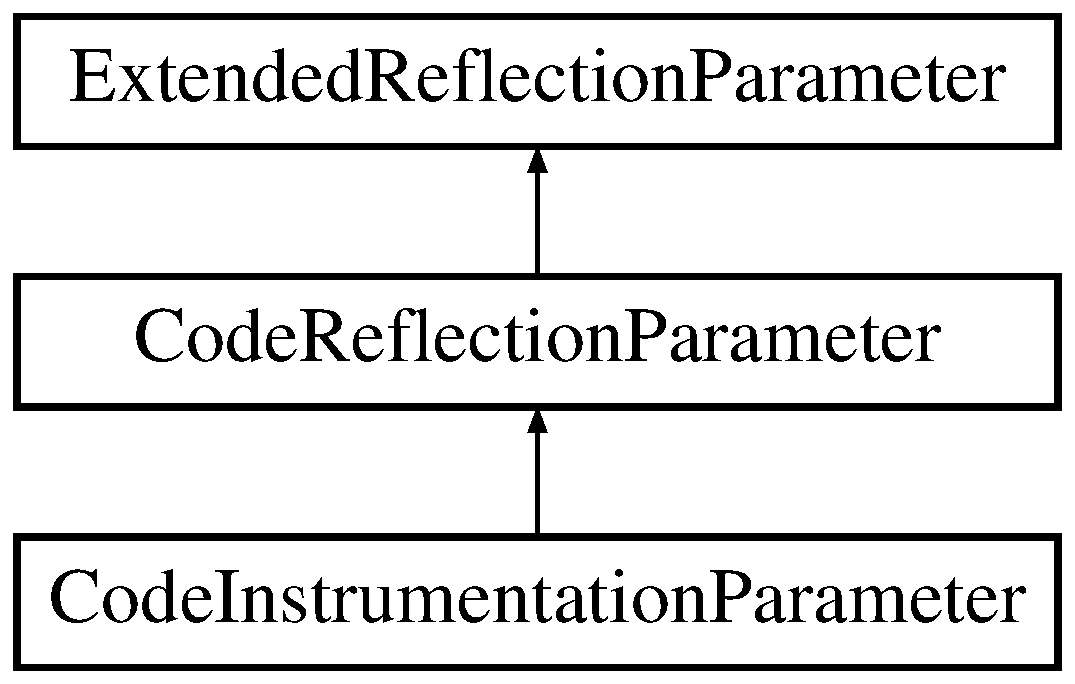
\includegraphics[height=3cm]{class_extended_reflection_parameter}
\end{center}
\end{figure}
\subsection*{Public Member Functions}
\begin{CompactItemize}
\item 
\hyperlink{class_extended_reflection_parameter_acff3f8d93cc250281f0f73bff3422e1}{getDeclaringClass} ()
\item 
\hyperlink{class_extended_reflection_parameter_23ecbde357f7f6bde5a50f876334a74d}{getClass} ()
\item 
\hyperlink{class_extended_reflection_parameter_af67f978eb2fb55cd1835c75ab86feba}{getDeclaringFunction} ()
\end{CompactItemize}
\subsection*{Protected Member Functions}
\begin{CompactItemize}
\item 
\hyperlink{class_extended_reflection_parameter_6b56ec198bc6a5b5a72076e4e7c19e29}{createExtendedReflectionClass} (ReflectionClass \$objOriginalReflectionClass)
\item 
\hyperlink{class_extended_reflection_parameter_ec7c1d4b204b6e3a6291d3b867afb688}{createExtendedReflectionMethod} (ReflectionMethod \$objOriginalReflectionMethod)
\item 
\hyperlink{class_extended_reflection_parameter_b23ad87d3ac2f376c1a133ca6d27f031}{createExtendedReflectionFunction} (ReflectionFunction \$objOriginalReflectionFunction)
\end{CompactItemize}


\subsection{Detailed Description}
Class what make possible and easy extend reflection parameter

Reflection classes can be a problem because the reflection methods what return objects will return the original reflection object and not the extended version of it. So it is necessary to create methods what convert the original methods to return the extended version of the objects.

\begin{Desc}
\item[Author:]Thiago Henrique Ramos da Mata $<$\href{mailto:thiago.henrique.mata@gmail.com}{\tt thiago.henrique.mata@gmail.com}$>$ \end{Desc}


\subsection{Member Function Documentation}
\hypertarget{class_extended_reflection_parameter_6b56ec198bc6a5b5a72076e4e7c19e29}{
\index{ExtendedReflectionParameter@{ExtendedReflectionParameter}!createExtendedReflectionClass@{createExtendedReflectionClass}}
\index{createExtendedReflectionClass@{createExtendedReflectionClass}!ExtendedReflectionParameter@{ExtendedReflectionParameter}}
\subsubsection[{createExtendedReflectionClass}]{\setlength{\rightskip}{0pt plus 5cm}createExtendedReflectionClass (ReflectionClass \$ {\em objOriginalReflectionClass})\hspace{0.3cm}{\tt  \mbox{[}protected\mbox{]}}}}
\label{class_extended_reflection_parameter_6b56ec198bc6a5b5a72076e4e7c19e29}


Convert a reflection class into a extended reflection class

This is the method what should be replaced when this class be extended.

\begin{Desc}
\item[Parameters:]
\begin{description}
\item[{\em ReflectionClass}]\$objOriginalReflectionClass \end{description}
\end{Desc}
\begin{Desc}
\item[Returns:]\hyperlink{class_extended_reflection_class}{ExtendedReflectionClass} \end{Desc}


Reimplemented in \hyperlink{class_code_instrumentation_parameter_6b56ec198bc6a5b5a72076e4e7c19e29}{CodeInstrumentationParameter}, and \hyperlink{class_code_reflection_parameter_6b56ec198bc6a5b5a72076e4e7c19e29}{CodeReflectionParameter}.

\begin{Code}\begin{verbatim}65         {
66                 return new ExtendedReflectionClass( $objOriginalReflectionClass->getName() );
67         }
\end{verbatim}
\end{Code}


\hypertarget{class_extended_reflection_parameter_b23ad87d3ac2f376c1a133ca6d27f031}{
\index{ExtendedReflectionParameter@{ExtendedReflectionParameter}!createExtendedReflectionFunction@{createExtendedReflectionFunction}}
\index{createExtendedReflectionFunction@{createExtendedReflectionFunction}!ExtendedReflectionParameter@{ExtendedReflectionParameter}}
\subsubsection[{createExtendedReflectionFunction}]{\setlength{\rightskip}{0pt plus 5cm}createExtendedReflectionFunction (ReflectionFunction \$ {\em objOriginalReflectionFunction})\hspace{0.3cm}{\tt  \mbox{[}protected\mbox{]}}}}
\label{class_extended_reflection_parameter_b23ad87d3ac2f376c1a133ca6d27f031}


Convert a reflection function into a extended reflection function

This is the method what should be replaced when this class be extended.

\begin{Desc}
\item[Parameters:]
\begin{description}
\item[{\em ReflectionFunction}]\$objOriginalReflectionFunction \end{description}
\end{Desc}
\begin{Desc}
\item[Returns:]\hyperlink{class_extended_reflection_function}{ExtendedReflectionFunction} \end{Desc}


Reimplemented in \hyperlink{class_code_instrumentation_parameter_b23ad87d3ac2f376c1a133ca6d27f031}{CodeInstrumentationParameter}, and \hyperlink{class_code_reflection_parameter_b23ad87d3ac2f376c1a133ca6d27f031}{CodeReflectionParameter}.

\begin{Code}\begin{verbatim}93         {
94                 if( $objOriginalReflectionFunction instanceof ReflectionMethod )
95                 {
96                         return new ExtendedReflectionMethod( $objOriginalReflectionFunction->getName() );
97                 }
98                 else
99                 {
100                         return new ExtendedReflectionFunction( $objOriginalReflectionFunction->getName() );
101                 }
102         }
\end{verbatim}
\end{Code}


\hypertarget{class_extended_reflection_parameter_ec7c1d4b204b6e3a6291d3b867afb688}{
\index{ExtendedReflectionParameter@{ExtendedReflectionParameter}!createExtendedReflectionMethod@{createExtendedReflectionMethod}}
\index{createExtendedReflectionMethod@{createExtendedReflectionMethod}!ExtendedReflectionParameter@{ExtendedReflectionParameter}}
\subsubsection[{createExtendedReflectionMethod}]{\setlength{\rightskip}{0pt plus 5cm}createExtendedReflectionMethod (ReflectionMethod \$ {\em objOriginalReflectionMethod})\hspace{0.3cm}{\tt  \mbox{[}protected\mbox{]}}}}
\label{class_extended_reflection_parameter_ec7c1d4b204b6e3a6291d3b867afb688}


Convert a reflection method into a extended reflection method

This is the method what should be replaced when this class be extended.

\begin{Desc}
\item[Parameters:]
\begin{description}
\item[{\em ReflectionMethod}]\$objOriginalReflectionMethod \end{description}
\end{Desc}
\begin{Desc}
\item[Returns:]\hyperlink{class_extended_reflection_method}{ExtendedReflectionMethod} \end{Desc}


Reimplemented in \hyperlink{class_code_instrumentation_parameter_ec7c1d4b204b6e3a6291d3b867afb688}{CodeInstrumentationParameter}, and \hyperlink{class_code_reflection_parameter_ec7c1d4b204b6e3a6291d3b867afb688}{CodeReflectionParameter}.

\begin{Code}\begin{verbatim}79         {
80                 return new ExtendedReflectionMethod( $this->getName() , $objOriginalReflectionMethod->getName() );
81         }
\end{verbatim}
\end{Code}


\hypertarget{class_extended_reflection_parameter_23ecbde357f7f6bde5a50f876334a74d}{
\index{ExtendedReflectionParameter@{ExtendedReflectionParameter}!getClass@{getClass}}
\index{getClass@{getClass}!ExtendedReflectionParameter@{ExtendedReflectionParameter}}
\subsubsection[{getClass}]{\setlength{\rightskip}{0pt plus 5cm}getClass ()\hspace{0.3cm}{\tt  \mbox{[}final\mbox{]}}}}
\label{class_extended_reflection_parameter_23ecbde357f7f6bde5a50f876334a74d}


Get the class type of the reflected parameter

\begin{Desc}
\item[Returns:]\hyperlink{class_extended_reflection_class}{ExtendedReflectionClass} \end{Desc}


\begin{Code}\begin{verbatim}37     {
38         if( parent::getClass() == null )
39         {
40                 return null;
41         }
42         return $this->createExtendedReflectionClass( parent::getClass() );
43     }
\end{verbatim}
\end{Code}


\hypertarget{class_extended_reflection_parameter_acff3f8d93cc250281f0f73bff3422e1}{
\index{ExtendedReflectionParameter@{ExtendedReflectionParameter}!getDeclaringClass@{getDeclaringClass}}
\index{getDeclaringClass@{getDeclaringClass}!ExtendedReflectionParameter@{ExtendedReflectionParameter}}
\subsubsection[{getDeclaringClass}]{\setlength{\rightskip}{0pt plus 5cm}getDeclaringClass ()\hspace{0.3cm}{\tt  \mbox{[}final\mbox{]}}}}
\label{class_extended_reflection_parameter_acff3f8d93cc250281f0f73bff3422e1}


Get the class owner of the reflected parameter

\begin{Desc}
\item[Returns:]\hyperlink{class_extended_reflection_class}{ExtendedReflectionClass} \end{Desc}


\begin{Code}\begin{verbatim}27     {
28         return $this->createExtendedReflectionClass( parent::getDeclaringClass() );
29     }
\end{verbatim}
\end{Code}


\hypertarget{class_extended_reflection_parameter_af67f978eb2fb55cd1835c75ab86feba}{
\index{ExtendedReflectionParameter@{ExtendedReflectionParameter}!getDeclaringFunction@{getDeclaringFunction}}
\index{getDeclaringFunction@{getDeclaringFunction}!ExtendedReflectionParameter@{ExtendedReflectionParameter}}
\subsubsection[{getDeclaringFunction}]{\setlength{\rightskip}{0pt plus 5cm}getDeclaringFunction ()\hspace{0.3cm}{\tt  \mbox{[}final\mbox{]}}}}
\label{class_extended_reflection_parameter_af67f978eb2fb55cd1835c75ab86feba}


Get the declarion function of the reflected function

\begin{Desc}
\item[Returns:]\hyperlink{class_extended_reflection_function}{ExtendedReflectionFunction} \end{Desc}


\begin{Code}\begin{verbatim}51     {
52         $objReflectionFunction = $this->createExtendedReflectionFunction( parent::getDeclaringFunction() );
53     }
\end{verbatim}
\end{Code}




The documentation for this class was generated from the following file:\begin{CompactItemize}
\item 
components/extendedReflection/\hyperlink{_extended_reflection_parameter_8class_8php}{ExtendedReflectionParameter.class.php}\end{CompactItemize}

\hypertarget{class_extended_reflection_property}{
\section{ExtendedReflectionProperty Class Reference}
\label{class_extended_reflection_property}\index{ExtendedReflectionProperty@{ExtendedReflectionProperty}}
}
Inheritance diagram for ExtendedReflectionProperty::\begin{figure}[H]
\begin{center}
\leavevmode
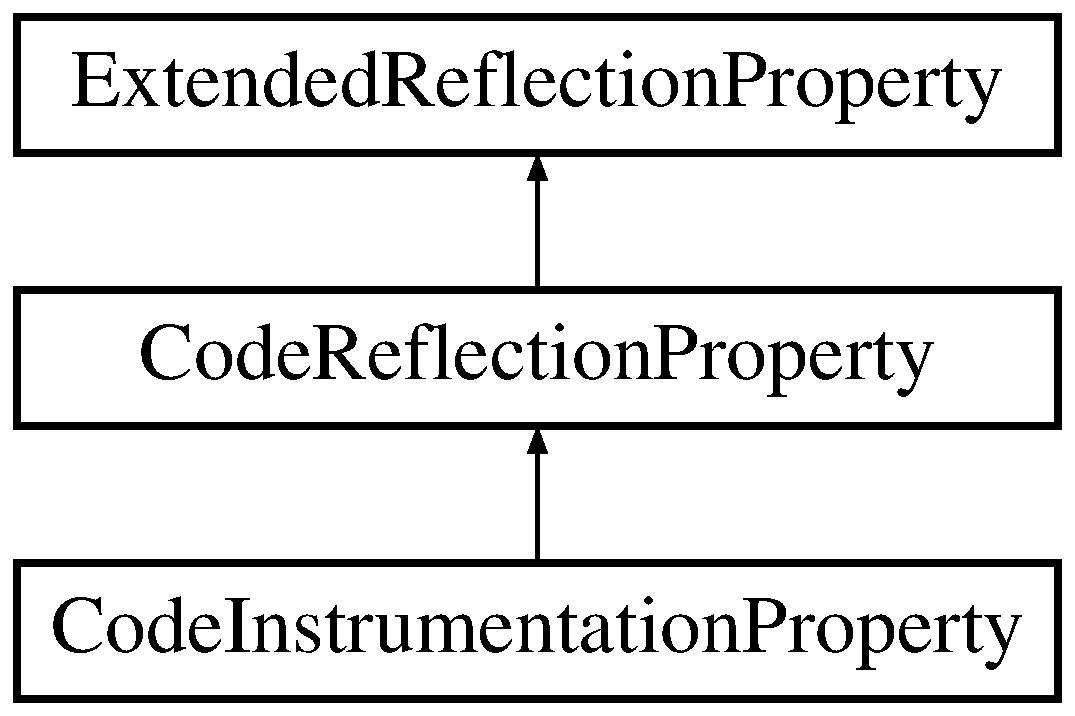
\includegraphics[height=3cm]{class_extended_reflection_property}
\end{center}
\end{figure}
\subsection*{Public Member Functions}
\begin{CompactItemize}
\item 
\hyperlink{class_extended_reflection_property_af1e7fdb7af7548692400dcad6c85c65}{getDeclaringClass} ()
\end{CompactItemize}
\subsection*{Protected Member Functions}
\begin{CompactItemize}
\item 
\hyperlink{class_extended_reflection_property_05c178f6fef194d390db8312f9595d93}{createExtendedReflectionClass} (ReflectionClass \$objOriginalReflectionClass)
\end{CompactItemize}


\subsection{Member Function Documentation}
\hypertarget{class_extended_reflection_property_05c178f6fef194d390db8312f9595d93}{
\index{ExtendedReflectionProperty@{ExtendedReflectionProperty}!createExtendedReflectionClass@{createExtendedReflectionClass}}
\index{createExtendedReflectionClass@{createExtendedReflectionClass}!ExtendedReflectionProperty@{ExtendedReflectionProperty}}
\subsubsection[{createExtendedReflectionClass}]{\setlength{\rightskip}{0pt plus 5cm}ExtendedReflectionProperty::createExtendedReflectionClass (ReflectionClass \$ {\em objOriginalReflectionClass})\hspace{0.3cm}{\tt  \mbox{[}protected\mbox{]}}}}
\label{class_extended_reflection_property_05c178f6fef194d390db8312f9595d93}


Convert a reflection class into a extended reflection class

This is the method what should be replaced when this class be extended.

\begin{Desc}
\item[Parameters:]
\begin{description}
\item[{\em ReflectionClass}]\$objOriginalReflectionClass \end{description}
\end{Desc}
\begin{Desc}
\item[Returns:]\hyperlink{class_extended_reflection_class}{ExtendedReflectionClass} \end{Desc}


Reimplemented in \hyperlink{class_code_instrumentation_property_192bcd477b39d69274c9a7db05cc606d}{CodeInstrumentationProperty}, and \hyperlink{class_code_reflection_property_ada66f395b16622378963471801f11ad}{CodeReflectionProperty}.\hypertarget{class_extended_reflection_property_af1e7fdb7af7548692400dcad6c85c65}{
\index{ExtendedReflectionProperty@{ExtendedReflectionProperty}!getDeclaringClass@{getDeclaringClass}}
\index{getDeclaringClass@{getDeclaringClass}!ExtendedReflectionProperty@{ExtendedReflectionProperty}}
\subsubsection[{getDeclaringClass}]{\setlength{\rightskip}{0pt plus 5cm}ExtendedReflectionProperty::getDeclaringClass ()\hspace{0.3cm}{\tt  \mbox{[}final\mbox{]}}}}
\label{class_extended_reflection_property_af1e7fdb7af7548692400dcad6c85c65}


Get the class owner of the reflected parameter

\begin{Desc}
\item[Returns:]\hyperlink{class_extended_reflection_class}{ExtendedReflectionClass} \end{Desc}


The documentation for this class was generated from the following file:\begin{CompactItemize}
\item 
components/extendedReflection/\hyperlink{_extended_reflection_property_8class_8php}{ExtendedReflectionProperty.class.php}\end{CompactItemize}

\hypertarget{class_fatorial}{
\section{Fatorial Class Reference}
\label{class_fatorial}\index{Fatorial@{Fatorial}}
}
\subsection*{Static Public Member Functions}
\begin{CompactItemize}
\item 
static \hyperlink{class_fatorial_72d167f440f3d1ac6d5d241195ea245c}{play} (\$n)
\end{CompactItemize}


\subsection{Member Function Documentation}
\hypertarget{class_fatorial_72d167f440f3d1ac6d5d241195ea245c}{
\index{Fatorial@{Fatorial}!play@{play}}
\index{play@{play}!Fatorial@{Fatorial}}
\subsubsection[{play}]{\setlength{\rightskip}{0pt plus 5cm}static Fatorial::play (\$ {\em n})\hspace{0.3cm}{\tt  \mbox{[}static\mbox{]}}}}
\label{class_fatorial_72d167f440f3d1ac6d5d241195ea245c}


calc the fatorial of the value received

\begin{Desc}
\item[Parameters:]
\begin{description}
\item[{\em integer}]\$n \end{description}
\end{Desc}
\begin{Desc}
\item[Returns:]integer \end{Desc}


The documentation for this class was generated from the following file:\begin{CompactItemize}
\item 
examples/Fatorial/\hyperlink{_fatorial_8php}{Fatorial.php}\end{CompactItemize}

\hypertarget{class_history}{
\section{History Class Reference}
\label{class_history}\index{History@{History}}
}
\subsection*{Public Member Functions}
\begin{CompactItemize}
\item 
\hyperlink{class_history_b6e145cb886ba3fdbca030285b402894}{\_\-\_\-construct} ()
\end{CompactItemize}


\subsection{Constructor \& Destructor Documentation}
\hypertarget{class_history_b6e145cb886ba3fdbca030285b402894}{
\index{History@{History}!\_\-\_\-construct@{\_\-\_\-construct}}
\index{\_\-\_\-construct@{\_\-\_\-construct}!History@{History}}
\subsubsection[{\_\-\_\-construct}]{\setlength{\rightskip}{0pt plus 5cm}History::\_\-\_\-construct ()}}
\label{class_history_b6e145cb886ba3fdbca030285b402894}




The documentation for this class was generated from the following file:\begin{CompactItemize}
\item 
examples/ThreeLittlePigs/\hyperlink{_history_8class_8php}{History.class.php}\end{CompactItemize}

\hypertarget{class_house}{
\section{House Class Reference}
\label{class_house}\index{House@{House}}
}
\subsection*{Public Member Functions}
\begin{CompactItemize}
\item 
\hyperlink{class_house_48d409343c54e747174ffaf5911b2cd9}{setType} (\$strType)
\item 
\hyperlink{class_house_830b5c75df72b32396701bc563fbe3c7}{getType} ()
\item 
\hyperlink{class_house_cd0f1de87d37a838789035eaf58f17b0}{colapse} ()
\item 
\hyperlink{class_house_17f029203fb995258650c19e2616e669}{isColapsed} ()
\item 
\hyperlink{class_house_5fbf3e8f1af77b77aba13d24cd3218e0}{setPig} (\hyperlink{class_little_pig}{LittlePig} \$objPig)
\item 
\hyperlink{class_house_6b0a38021f87bca50710aba818be2809}{getPig} ()
\item 
\hyperlink{class_house_20552b3b737f2189821f0362e2bd9cee}{getBlowBy} (\hyperlink{class_wolf}{Wolf} \$objWolf)
\end{CompactItemize}
\subsection*{Protected Attributes}
\begin{CompactItemize}
\item 
\hyperlink{class_house_ac9a08cb422ab9a398d451299b054e28}{\$strType}
\item 
\hyperlink{class_house_eeadc4737b5ad49aa0a56c7bbbafdffe}{\$objPig}
\item 
\hyperlink{class_house_2eaf201bec0ce5594be8a5eb8e71b5b9}{\$booIsColapsed} = false
\end{CompactItemize}


\subsection{Detailed Description}
\hyperlink{class_house}{House} of the little pigs to the example of the code to diagram

\begin{Desc}
\item[Author:]Thiago Henrique Ramos da Mata $<$\href{mailto:thiago.henrique.mata@gmail.com}{\tt thiago.henrique.mata@gmail.com}$>$ \end{Desc}


\subsection{Member Function Documentation}
\hypertarget{class_house_cd0f1de87d37a838789035eaf58f17b0}{
\index{House@{House}!colapse@{colapse}}
\index{colapse@{colapse}!House@{House}}
\subsubsection[{colapse}]{\setlength{\rightskip}{0pt plus 5cm}colapse ()}}
\label{class_house_cd0f1de87d37a838789035eaf58f17b0}


Make the house colapse

\begin{Desc}
\item[Returns:]\hyperlink{class_house}{House} me \end{Desc}


\begin{Code}\begin{verbatim}69     {
70         $this->booIsColapsed = true;
71         return $this;
72     }
\end{verbatim}
\end{Code}


\hypertarget{class_house_20552b3b737f2189821f0362e2bd9cee}{
\index{House@{House}!getBlowBy@{getBlowBy}}
\index{getBlowBy@{getBlowBy}!House@{House}}
\subsubsection[{getBlowBy}]{\setlength{\rightskip}{0pt plus 5cm}getBlowBy ({\bf Wolf} \$ {\em objWolf})}}
\label{class_house_20552b3b737f2189821f0362e2bd9cee}


Receive a blow from the wolf.

If the house has the type \char`\"{}Brick\char`\"{} the house dont colapse the the pig, owner of the house it is waked up by the wolf noise. But, if the house has not, the house colapse.

Return {\tt true} if the house is colapsed and {\tt false} if not

\begin{Desc}
\item[Parameters:]
\begin{description}
\item[{\em \hyperlink{class_wolf}{Wolf}}]\$objWolf \end{description}
\end{Desc}
\begin{Desc}
\item[Returns:]boolean \end{Desc}


\begin{Code}\begin{verbatim}128     {
129         if( $this->getType() == "Brick" )
130         {
131             $this->getPig()->wakeUpBy( $objWolf );
132         }
133         else
134         {
135             $this->colapse();
136         }
137         return $this->isColapsed();
138     }
\end{verbatim}
\end{Code}


\hypertarget{class_house_6b0a38021f87bca50710aba818be2809}{
\index{House@{House}!getPig@{getPig}}
\index{getPig@{getPig}!House@{House}}
\subsubsection[{getPig}]{\setlength{\rightskip}{0pt plus 5cm}getPig ()}}
\label{class_house_6b0a38021f87bca50710aba818be2809}


Get the little pig onwer of the house

\begin{Desc}
\item[See also:]House::setPig( LittlePig ) 

House-$>$objPig \end{Desc}
\begin{Desc}
\item[Returns:]\hyperlink{class_little_pig}{LittlePig} \end{Desc}


\begin{Code}\begin{verbatim}107     {
108         return $this->objPig;
109     }
\end{verbatim}
\end{Code}


\hypertarget{class_house_830b5c75df72b32396701bc563fbe3c7}{
\index{House@{House}!getType@{getType}}
\index{getType@{getType}!House@{House}}
\subsubsection[{getType}]{\setlength{\rightskip}{0pt plus 5cm}getType ()}}
\label{class_house_830b5c75df72b32396701bc563fbe3c7}


get the type of the house

\begin{Desc}
\item[See also:]House::setType( string ) 

House-$>$strType \end{Desc}
\begin{Desc}
\item[Returns:]string \end{Desc}


\begin{Code}\begin{verbatim}59     {
60         return $this->strType;
61     }
\end{verbatim}
\end{Code}


\hypertarget{class_house_17f029203fb995258650c19e2616e669}{
\index{House@{House}!isColapsed@{isColapsed}}
\index{isColapsed@{isColapsed}!House@{House}}
\subsubsection[{isColapsed}]{\setlength{\rightskip}{0pt plus 5cm}isColapsed ()}}
\label{class_house_17f029203fb995258650c19e2616e669}


Return {\tt true} if the house is colapsed and {\tt false} if not

\begin{Desc}
\item[Returns:]boolean \end{Desc}


\begin{Code}\begin{verbatim}81     {
82         return $this->booIsColapsed;
83     }
\end{verbatim}
\end{Code}


\hypertarget{class_house_5fbf3e8f1af77b77aba13d24cd3218e0}{
\index{House@{House}!setPig@{setPig}}
\index{setPig@{setPig}!House@{House}}
\subsubsection[{setPig}]{\setlength{\rightskip}{0pt plus 5cm}setPig ({\bf LittlePig} \$ {\em objPig})}}
\label{class_house_5fbf3e8f1af77b77aba13d24cd3218e0}


Set the little pig owner of the house

\begin{Desc}
\item[See also:]\hyperlink{class_house_6b0a38021f87bca50710aba818be2809}{House::getPig()} 

House-$>$objPig \end{Desc}
\begin{Desc}
\item[Parameters:]
\begin{description}
\item[{\em \hyperlink{class_little_pig}{LittlePig}}]\$objPig \end{description}
\end{Desc}
\begin{Desc}
\item[Returns:]\hyperlink{class_house}{House} me \end{Desc}


\begin{Code}\begin{verbatim}94     {
95         $this->objPig = $objPig;
96         return $this;
97     }
\end{verbatim}
\end{Code}


\hypertarget{class_house_48d409343c54e747174ffaf5911b2cd9}{
\index{House@{House}!setType@{setType}}
\index{setType@{setType}!House@{House}}
\subsubsection[{setType}]{\setlength{\rightskip}{0pt plus 5cm}setType (\$ {\em strType})}}
\label{class_house_48d409343c54e747174ffaf5911b2cd9}


Set the type of the house

\begin{Desc}
\item[See also:]\hyperlink{class_house_830b5c75df72b32396701bc563fbe3c7}{House::getType()} 

House-$>$strType \end{Desc}
\begin{Desc}
\item[Parameters:]
\begin{description}
\item[{\em string}]\$strType \end{description}
\end{Desc}
\begin{Desc}
\item[Returns:]\hyperlink{class_house}{House} me \end{Desc}


\begin{Code}\begin{verbatim}46     {
47         $this->strType = $strType;
48         return $this;
49     }
\end{verbatim}
\end{Code}




\subsection{Member Data Documentation}
\hypertarget{class_house_2eaf201bec0ce5594be8a5eb8e71b5b9}{
\index{House@{House}!\$booIsColapsed@{\$booIsColapsed}}
\index{\$booIsColapsed@{\$booIsColapsed}!House@{House}}
\subsubsection[{\$booIsColapsed}]{\setlength{\rightskip}{0pt plus 5cm}\$booIsColapsed = false\hspace{0.3cm}{\tt  \mbox{[}protected\mbox{]}}}}
\label{class_house_2eaf201bec0ce5594be8a5eb8e71b5b9}


This controlls if the house has colapsed

boolean \hypertarget{class_house_eeadc4737b5ad49aa0a56c7bbbafdffe}{
\index{House@{House}!\$objPig@{\$objPig}}
\index{\$objPig@{\$objPig}!House@{House}}
\subsubsection[{\$objPig}]{\setlength{\rightskip}{0pt plus 5cm}\$objPig\hspace{0.3cm}{\tt  \mbox{[}protected\mbox{]}}}}
\label{class_house_eeadc4737b5ad49aa0a56c7bbbafdffe}


Pig owner of the house

\hyperlink{class_little_pig}{LittlePig} \hypertarget{class_house_ac9a08cb422ab9a398d451299b054e28}{
\index{House@{House}!\$strType@{\$strType}}
\index{\$strType@{\$strType}!House@{House}}
\subsubsection[{\$strType}]{\setlength{\rightskip}{0pt plus 5cm}\$strType\hspace{0.3cm}{\tt  \mbox{[}protected\mbox{]}}}}
\label{class_house_ac9a08cb422ab9a398d451299b054e28}


Type of the house

string 

The documentation for this class was generated from the following file:\begin{CompactItemize}
\item 
examples/ThreeLittlePigs/\hyperlink{_house_8class_8php}{House.class.php}\end{CompactItemize}

\hypertarget{class_little_pig}{
\section{LittlePig Class Reference}
\label{class_little_pig}\index{LittlePig@{LittlePig}}
}
\subsection*{Public Member Functions}
\begin{CompactItemize}
\item 
\hyperlink{class_little_pig_0d2d86aa9b7de45757e2d29384b1e549}{say} (\$strText)
\item 
\hyperlink{class_little_pig_c05d9184d52b7a34210a801767bef213}{setName} (\$strName)
\item 
\hyperlink{class_little_pig_082ad68f4d76b0c185027dcbf3a4dc42}{buildHouse} (\$strType)
\item 
\hyperlink{class_little_pig_24a3c5baa4accd4da966da7437d92a6d}{getHouse} ()
\item 
\hyperlink{class_little_pig_11dd4caed12c9780c2dd944d6b024109}{happyEverAfter} ()
\item 
\hyperlink{class_little_pig_990f0b86c82d36f1f94ff331db475c85}{isEaten} ()
\item 
\hyperlink{class_little_pig_ec29070d2544b3cfe0447dcbc5e6c199}{isKilled} ()
\item 
\hyperlink{class_little_pig_ec9bcb744b45ac0a7b30e9e53bddb4d4}{wakeUpBy} (\hyperlink{class_wolf}{Wolf} \$objWolf)
\end{CompactItemize}
\subsection*{Protected Attributes}
\begin{CompactItemize}
\item 
\hyperlink{class_little_pig_90edf7538a74be8ac5ce46baaf203382}{\$strName}
\item 
\hyperlink{class_little_pig_79150187cd5131ac2aa384dc660f3f65}{\$objHouse}
\end{CompactItemize}


\subsection{Detailed Description}
Little pigs of the example of the code to diagram

\begin{Desc}
\item[Author:]Thiago Henrique Ramos da Mata $<$\href{mailto:thiago.henrique.mata@gmail.com}{\tt thiago.henrique.mata@gmail.com}$>$ \end{Desc}


\subsection{Member Function Documentation}
\hypertarget{class_little_pig_082ad68f4d76b0c185027dcbf3a4dc42}{
\index{LittlePig@{LittlePig}!buildHouse@{buildHouse}}
\index{buildHouse@{buildHouse}!LittlePig@{LittlePig}}
\subsubsection[{buildHouse}]{\setlength{\rightskip}{0pt plus 5cm}buildHouse (\$ {\em strType})}}
\label{class_little_pig_082ad68f4d76b0c185027dcbf3a4dc42}


Make the Little Pig buid the house of the received type

\begin{Desc}
\item[Parameters:]
\begin{description}
\item[{\em string}]\$strType type of the house \end{description}
\end{Desc}
\begin{Desc}
\item[Returns:]\hyperlink{class_little_pig}{LittlePig} me \end{Desc}


\begin{Code}\begin{verbatim}61     {
62         $objHouse = new House();
63         $objHouse->setType( $strType );
64         $this->objHouse = $objHouse;
65         $this->objHouse->setPig( $this );
66         return $this;
67     }
\end{verbatim}
\end{Code}


\hypertarget{class_little_pig_24a3c5baa4accd4da966da7437d92a6d}{
\index{LittlePig@{LittlePig}!getHouse@{getHouse}}
\index{getHouse@{getHouse}!LittlePig@{LittlePig}}
\subsubsection[{getHouse}]{\setlength{\rightskip}{0pt plus 5cm}getHouse ()}}
\label{class_little_pig_24a3c5baa4accd4da966da7437d92a6d}


Get the house of the little pig

\begin{Desc}
\item[Returns:]\hyperlink{class_house}{House} \end{Desc}


\begin{Code}\begin{verbatim}75     {
76         return $this->objHouse;
77     }
\end{verbatim}
\end{Code}


\hypertarget{class_little_pig_11dd4caed12c9780c2dd944d6b024109}{
\index{LittlePig@{LittlePig}!happyEverAfter@{happyEverAfter}}
\index{happyEverAfter@{happyEverAfter}!LittlePig@{LittlePig}}
\subsubsection[{happyEverAfter}]{\setlength{\rightskip}{0pt plus 5cm}happyEverAfter ()}}
\label{class_little_pig_11dd4caed12c9780c2dd944d6b024109}


Little Pig celebrate the happy ever after 

\begin{Code}\begin{verbatim}84     {
85         $this->say( "i am happy ever after!" );
86     }
\end{verbatim}
\end{Code}


\hypertarget{class_little_pig_990f0b86c82d36f1f94ff331db475c85}{
\index{LittlePig@{LittlePig}!isEaten@{isEaten}}
\index{isEaten@{isEaten}!LittlePig@{LittlePig}}
\subsubsection[{isEaten}]{\setlength{\rightskip}{0pt plus 5cm}isEaten ()}}
\label{class_little_pig_990f0b86c82d36f1f94ff331db475c85}


Little pig it is eaten 

\begin{Code}\begin{verbatim}92     {
93 
94     }
\end{verbatim}
\end{Code}


\hypertarget{class_little_pig_ec29070d2544b3cfe0447dcbc5e6c199}{
\index{LittlePig@{LittlePig}!isKilled@{isKilled}}
\index{isKilled@{isKilled}!LittlePig@{LittlePig}}
\subsubsection[{isKilled}]{\setlength{\rightskip}{0pt plus 5cm}isKilled ()}}
\label{class_little_pig_ec29070d2544b3cfe0447dcbc5e6c199}


Little pig is killed 

\begin{Code}\begin{verbatim}101     {
102 
103     }
\end{verbatim}
\end{Code}


\hypertarget{class_little_pig_0d2d86aa9b7de45757e2d29384b1e549}{
\index{LittlePig@{LittlePig}!say@{say}}
\index{say@{say}!LittlePig@{LittlePig}}
\subsubsection[{say}]{\setlength{\rightskip}{0pt plus 5cm}say (\$ {\em strText})}}
\label{class_little_pig_0d2d86aa9b7de45757e2d29384b1e549}


The pig speak the received text

\begin{Desc}
\item[Parameters:]
\begin{description}
\item[{\em string}]\$strText \end{description}
\end{Desc}
\begin{Desc}
\item[Returns:]\hyperlink{class_little_pig}{LittlePig} \end{Desc}


\begin{Code}\begin{verbatim}37     {
38         print "pig say: " . $strText . "<br/>\n";
39         return $this;
40     }
\end{verbatim}
\end{Code}


\hypertarget{class_little_pig_c05d9184d52b7a34210a801767bef213}{
\index{LittlePig@{LittlePig}!setName@{setName}}
\index{setName@{setName}!LittlePig@{LittlePig}}
\subsubsection[{setName}]{\setlength{\rightskip}{0pt plus 5cm}setName (\$ {\em strName})}}
\label{class_little_pig_c05d9184d52b7a34210a801767bef213}


Set the Little Pig name

\begin{Desc}
\item[Parameters:]
\begin{description}
\item[{\em string}]\$strName \end{description}
\end{Desc}
\begin{Desc}
\item[Returns:]\hyperlink{class_little_pig}{LittlePig} me \end{Desc}


\begin{Code}\begin{verbatim}49     {
50         $this->strName = $strName;
51         return $this;
52     }
\end{verbatim}
\end{Code}


\hypertarget{class_little_pig_ec9bcb744b45ac0a7b30e9e53bddb4d4}{
\index{LittlePig@{LittlePig}!wakeUpBy@{wakeUpBy}}
\index{wakeUpBy@{wakeUpBy}!LittlePig@{LittlePig}}
\subsubsection[{wakeUpBy}]{\setlength{\rightskip}{0pt plus 5cm}wakeUpBy ({\bf Wolf} \$ {\em objWolf})}}
\label{class_little_pig_ec9bcb744b45ac0a7b30e9e53bddb4d4}


Little pig is wake up by the wolf

1. little pig kill the wolf 2. little pig is happy ever after 

\begin{Code}\begin{verbatim}114     {
115         $objWolf->isKilled();
116         $this->happyEverAfter();
117     }
\end{verbatim}
\end{Code}




\subsection{Member Data Documentation}
\hypertarget{class_little_pig_79150187cd5131ac2aa384dc660f3f65}{
\index{LittlePig@{LittlePig}!\$objHouse@{\$objHouse}}
\index{\$objHouse@{\$objHouse}!LittlePig@{LittlePig}}
\subsubsection[{\$objHouse}]{\setlength{\rightskip}{0pt plus 5cm}\$objHouse\hspace{0.3cm}{\tt  \mbox{[}protected\mbox{]}}}}
\label{class_little_pig_79150187cd5131ac2aa384dc660f3f65}


Little Pig \hyperlink{class_house}{House}

\hyperlink{class_house}{House} \hypertarget{class_little_pig_90edf7538a74be8ac5ce46baaf203382}{
\index{LittlePig@{LittlePig}!\$strName@{\$strName}}
\index{\$strName@{\$strName}!LittlePig@{LittlePig}}
\subsubsection[{\$strName}]{\setlength{\rightskip}{0pt plus 5cm}\$strName\hspace{0.3cm}{\tt  \mbox{[}protected\mbox{]}}}}
\label{class_little_pig_90edf7538a74be8ac5ce46baaf203382}


Little Pig name

string 

The documentation for this class was generated from the following file:\begin{CompactItemize}
\item 
examples/ThreeLittlePigs/\hyperlink{_pig_8class_8php}{Pig.class.php}\end{CompactItemize}

\hypertarget{class_wolf}{
\section{Wolf Class Reference}
\label{class_wolf}\index{Wolf@{Wolf}}
}
\subsection*{Public Member Functions}
\begin{CompactItemize}
\item 
\hyperlink{class_wolf_0d2d86aa9b7de45757e2d29384b1e549}{say} (\$strText)
\item 
\hyperlink{class_wolf_5f459b17559a1eca24d746db4f77fac0}{huff} ()
\item 
\hyperlink{class_wolf_b5eff6bb92e5551d9188160b85e5cc19}{puff} ()
\item 
\hyperlink{class_wolf_9aad8c39845a1148d9088c6c4249a5e6}{blowIt} (\hyperlink{class_house}{House} \$objHouse)
\item 
\hyperlink{class_wolf_ec29070d2544b3cfe0447dcbc5e6c199}{isKilled} ()
\end{CompactItemize}


\subsection{Detailed Description}
\hyperlink{class_wolf}{Wolf} of the example of the code to diagram

\begin{Desc}
\item[Author:]Thiago Henrique Ramos da Mata $<$\href{mailto:thiago.henrique.mata@gmail.com}{\tt thiago.henrique.mata@gmail.com}$>$ \end{Desc}


\subsection{Member Function Documentation}
\hypertarget{class_wolf_9aad8c39845a1148d9088c6c4249a5e6}{
\index{Wolf@{Wolf}!blowIt@{blowIt}}
\index{blowIt@{blowIt}!Wolf@{Wolf}}
\subsubsection[{blowIt}]{\setlength{\rightskip}{0pt plus 5cm}blowIt ({\bf House} \$ {\em objHouse})}}
\label{class_wolf_9aad8c39845a1148d9088c6c4249a5e6}


\hyperlink{class_wolf}{Wolf} blow the house 

\begin{Code}\begin{verbatim}48     {
49         if( $objHouse->getBlowBy( $this ) )
50         {
51             $objPig = $objHouse->getPig();
52             $objPig->isKilled();
53             $objPig->isEaten();
54         }
55     }
\end{verbatim}
\end{Code}


\hypertarget{class_wolf_5f459b17559a1eca24d746db4f77fac0}{
\index{Wolf@{Wolf}!huff@{huff}}
\index{huff@{huff}!Wolf@{Wolf}}
\subsubsection[{huff}]{\setlength{\rightskip}{0pt plus 5cm}huff ()}}
\label{class_wolf_5f459b17559a1eca24d746db4f77fac0}


\hyperlink{class_wolf}{Wolf} buff 

\begin{Code}\begin{verbatim}32     {
33 
34     }
\end{verbatim}
\end{Code}


\hypertarget{class_wolf_ec29070d2544b3cfe0447dcbc5e6c199}{
\index{Wolf@{Wolf}!isKilled@{isKilled}}
\index{isKilled@{isKilled}!Wolf@{Wolf}}
\subsubsection[{isKilled}]{\setlength{\rightskip}{0pt plus 5cm}isKilled ()}}
\label{class_wolf_ec29070d2544b3cfe0447dcbc5e6c199}


\hyperlink{class_wolf}{Wolf} is killed 

\begin{Code}\begin{verbatim}61     {
62         
63     }
\end{verbatim}
\end{Code}


\hypertarget{class_wolf_b5eff6bb92e5551d9188160b85e5cc19}{
\index{Wolf@{Wolf}!puff@{puff}}
\index{puff@{puff}!Wolf@{Wolf}}
\subsubsection[{puff}]{\setlength{\rightskip}{0pt plus 5cm}puff ()}}
\label{class_wolf_b5eff6bb92e5551d9188160b85e5cc19}


\hyperlink{class_wolf}{Wolf} puff 

\begin{Code}\begin{verbatim}40     {
41 
42     }
\end{verbatim}
\end{Code}


\hypertarget{class_wolf_0d2d86aa9b7de45757e2d29384b1e549}{
\index{Wolf@{Wolf}!say@{say}}
\index{say@{say}!Wolf@{Wolf}}
\subsubsection[{say}]{\setlength{\rightskip}{0pt plus 5cm}say (\$ {\em strText})}}
\label{class_wolf_0d2d86aa9b7de45757e2d29384b1e549}


\hyperlink{class_wolf}{Wolf} say the received text

\begin{Desc}
\item[Parameters:]
\begin{description}
\item[{\em string}]\$strText \end{description}
\end{Desc}
\begin{Desc}
\item[Returns:]\hyperlink{class_wolf}{Wolf} me \end{Desc}


\begin{Code}\begin{verbatim}23     {
24         print "wolf say: " . $strText . " <br/>\n";
25         return $this;
26     }
\end{verbatim}
\end{Code}




The documentation for this class was generated from the following file:\begin{CompactItemize}
\item 
examples/ThreeLittlePigs/\hyperlink{_wolf_8class_8php}{Wolf.class.php}\end{CompactItemize}

\hypertarget{class_xml_sequence}{
\section{XmlSequence Class Reference}
\label{class_xml_sequence}\index{XmlSequence@{XmlSequence}}
}
\subsection*{Public Member Functions}
\begin{CompactItemize}
\item 
\hyperlink{class_xml_sequence_953da102372c3cd12f7dfe7fb2f01bbd}{restart} ()
\item 
\hyperlink{class_xml_sequence_2b5e654d8a5559dc263da2d3bdbd043e}{setCallerPath} (\$strCallerPath)
\item 
\hyperlink{class_xml_sequence_197ff62ed0c4d22324218206147f25e4}{getCallerPath} ()
\item 
\hyperlink{class_xml_sequence_1b463d4b176c4798b8be4667262f0450}{setPublicPath} (\$strPublicPath)
\item 
\hyperlink{class_xml_sequence_156bcaa4792dca6a381621d68052ba32}{getPublicPath} ()
\item 
\hyperlink{class_xml_sequence_3cf549fbc588fc2bc0bbd74f818dfe91}{setMessages} (array \$arrMessages)
\item 
\hyperlink{class_xml_sequence_21cc38a9b7b19954bb0b8951b065ad11}{getMessages} ()
\item 
\hyperlink{class_xml_sequence_f46e383dc5728d4b072ac8299417dfed}{addMessage} (\hyperlink{class_xml_sequence_message}{XmlSequenceMessage} \$objMessage)
\item 
\hyperlink{class_xml_sequence_00aa28e395a3d00b7b15b1adebe092db}{setActors} (array \$arrActors)
\item 
\hyperlink{class_xml_sequence_dcce8335021177bac08889348f2a508e}{getActors} ()
\item 
\hyperlink{class_xml_sequence_4dcdb7d52d39bbdb4b9897c61570a064}{addActor} (\hyperlink{class_xml_sequence_actor}{XmlSequenceActor} \$objActor)
\end{CompactItemize}
\subsection*{Protected Attributes}
\begin{CompactItemize}
\item 
\hyperlink{class_xml_sequence_32c07693b6fb096943d6594bc198840d}{\$arrActors} = Array()
\item 
\hyperlink{class_xml_sequence_49575b42830f5ce6152e1cc4e2d934f3}{\$arrMessages} = Array()
\item 
\hyperlink{class_xml_sequence_81ff70d1bae4303f0454e8f76897cde7}{\$strCallerPath}
\item 
\hyperlink{class_xml_sequence_5a3049f005498d02e15be8e67c759ea1}{\$strPublicPath}
\end{CompactItemize}


\subsection{Member Function Documentation}
\hypertarget{class_xml_sequence_4dcdb7d52d39bbdb4b9897c61570a064}{
\index{XmlSequence@{XmlSequence}!addActor@{addActor}}
\index{addActor@{addActor}!XmlSequence@{XmlSequence}}
\subsubsection[{addActor}]{\setlength{\rightskip}{0pt plus 5cm}XmlSequence::addActor ({\bf XmlSequenceActor} \$ {\em objActor})}}
\label{class_xml_sequence_4dcdb7d52d39bbdb4b9897c61570a064}


Add a actor into the xml sequence object

\begin{Desc}
\item[See also:]\hyperlink{class_xml_sequence_00aa28e395a3d00b7b15b1adebe092db}{XmlSequence::setActors}( \hyperlink{class_xml_sequence_actor}{XmlSequenceActor}\mbox{[}\mbox{]} ) 

\hyperlink{class_xml_sequence_dcce8335021177bac08889348f2a508e}{XmlSequence::getActors()} \end{Desc}
\begin{Desc}
\item[Parameters:]
\begin{description}
\item[{\em \hyperlink{class_xml_sequence_actor}{XmlSequenceActor}}]\$objActor \end{description}
\end{Desc}
\begin{Desc}
\item[Returns:]\hyperlink{class_xml_sequence}{XmlSequence} me \end{Desc}
\hypertarget{class_xml_sequence_f46e383dc5728d4b072ac8299417dfed}{
\index{XmlSequence@{XmlSequence}!addMessage@{addMessage}}
\index{addMessage@{addMessage}!XmlSequence@{XmlSequence}}
\subsubsection[{addMessage}]{\setlength{\rightskip}{0pt plus 5cm}XmlSequence::addMessage ({\bf XmlSequenceMessage} \$ {\em objMessage})}}
\label{class_xml_sequence_f46e383dc5728d4b072ac8299417dfed}


Add a message into the xml sequence object

\begin{Desc}
\item[See also:]\hyperlink{class_xml_sequence_3cf549fbc588fc2bc0bbd74f818dfe91}{XmlSequence::setMessages}( \hyperlink{class_xml_sequence_message}{XmlSequenceMessage}\mbox{[}\mbox{]} ) 

\hyperlink{class_xml_sequence_21cc38a9b7b19954bb0b8951b065ad11}{XmlSequence::getMessages()} \end{Desc}
\begin{Desc}
\item[Parameters:]
\begin{description}
\item[{\em \hyperlink{class_xml_sequence_message}{XmlSequenceMessage}}]\$objMessage \end{description}
\end{Desc}
\begin{Desc}
\item[Returns:]\hyperlink{class_xml_sequence}{XmlSequence} me \end{Desc}
\hypertarget{class_xml_sequence_dcce8335021177bac08889348f2a508e}{
\index{XmlSequence@{XmlSequence}!getActors@{getActors}}
\index{getActors@{getActors}!XmlSequence@{XmlSequence}}
\subsubsection[{getActors}]{\setlength{\rightskip}{0pt plus 5cm}XmlSequence::getActors ()}}
\label{class_xml_sequence_dcce8335021177bac08889348f2a508e}


Get the array of xml sequence actors

\begin{Desc}
\item[See also:]\hyperlink{class_xml_sequence_00aa28e395a3d00b7b15b1adebe092db}{XmlSequence::setActors}( \hyperlink{class_xml_sequence_actor}{XmlSequenceActor}\mbox{[}\mbox{]} ) 

XmlSequence-$>$arrActors 

XmlSequence::addActor( XmlSequenceActor ) \end{Desc}
\begin{Desc}
\item[Returns:]\hyperlink{class_xml_sequence_actor}{XmlSequenceActor}\mbox{[}\mbox{]} \end{Desc}
\hypertarget{class_xml_sequence_197ff62ed0c4d22324218206147f25e4}{
\index{XmlSequence@{XmlSequence}!getCallerPath@{getCallerPath}}
\index{getCallerPath@{getCallerPath}!XmlSequence@{XmlSequence}}
\subsubsection[{getCallerPath}]{\setlength{\rightskip}{0pt plus 5cm}XmlSequence::getCallerPath ()}}
\label{class_xml_sequence_197ff62ed0c4d22324218206147f25e4}


Get the caller path

\begin{Desc}
\item[See also:]XmlSequence::setCallerPath( string ) 

XmlSequence-$>$strCallerPath \end{Desc}
\begin{Desc}
\item[Parameters:]
\begin{description}
\item[{\em string}]\$strCallerPath \end{description}
\end{Desc}
\begin{Desc}
\item[Returns:]string \end{Desc}
\hypertarget{class_xml_sequence_21cc38a9b7b19954bb0b8951b065ad11}{
\index{XmlSequence@{XmlSequence}!getMessages@{getMessages}}
\index{getMessages@{getMessages}!XmlSequence@{XmlSequence}}
\subsubsection[{getMessages}]{\setlength{\rightskip}{0pt plus 5cm}XmlSequence::getMessages ()}}
\label{class_xml_sequence_21cc38a9b7b19954bb0b8951b065ad11}


Get the array of xml sequence messages

\begin{Desc}
\item[See also:]\hyperlink{class_xml_sequence_3cf549fbc588fc2bc0bbd74f818dfe91}{XmlSequence::setMessages}( \hyperlink{class_xml_sequence_message}{XmlSequenceMessage}\mbox{[}\mbox{]} ) 

XmlSequence-$>$arrMessages 

XmlSequence::addMessage( XmlSequenceMessage ) \end{Desc}
\begin{Desc}
\item[Returns:]\hyperlink{class_xml_sequence_message}{XmlSequenceMessage}\mbox{[}\mbox{]} \end{Desc}
\hypertarget{class_xml_sequence_156bcaa4792dca6a381621d68052ba32}{
\index{XmlSequence@{XmlSequence}!getPublicPath@{getPublicPath}}
\index{getPublicPath@{getPublicPath}!XmlSequence@{XmlSequence}}
\subsubsection[{getPublicPath}]{\setlength{\rightskip}{0pt plus 5cm}XmlSequence::getPublicPath ()}}
\label{class_xml_sequence_156bcaa4792dca6a381621d68052ba32}


Get the \hyperlink{namespacepublic}{public} path

\begin{Desc}
\item[See also:]XmlSequence::setPublicPath( string ) 

XmlSequence-$>$strPublicPath \end{Desc}
\begin{Desc}
\item[Parameters:]
\begin{description}
\item[{\em string}]\$strPublicPath \end{description}
\end{Desc}
\begin{Desc}
\item[Returns:]string \end{Desc}
\hypertarget{class_xml_sequence_953da102372c3cd12f7dfe7fb2f01bbd}{
\index{XmlSequence@{XmlSequence}!restart@{restart}}
\index{restart@{restart}!XmlSequence@{XmlSequence}}
\subsubsection[{restart}]{\setlength{\rightskip}{0pt plus 5cm}XmlSequence::restart ()}}
\label{class_xml_sequence_953da102372c3cd12f7dfe7fb2f01bbd}


Restart xml sequence clean all the old actors and messages

\begin{Desc}
\item[Returns:]\hyperlink{class_xml_sequence}{XmlSequence} me \end{Desc}
\hypertarget{class_xml_sequence_00aa28e395a3d00b7b15b1adebe092db}{
\index{XmlSequence@{XmlSequence}!setActors@{setActors}}
\index{setActors@{setActors}!XmlSequence@{XmlSequence}}
\subsubsection[{setActors}]{\setlength{\rightskip}{0pt plus 5cm}XmlSequence::setActors (array \$ {\em arrActors})}}
\label{class_xml_sequence_00aa28e395a3d00b7b15b1adebe092db}


Set the array of xml sequence actors

\begin{Desc}
\item[See also:]\hyperlink{class_xml_sequence_dcce8335021177bac08889348f2a508e}{XmlSequence::getActors()} 

XmlSequence-$>$arrActors 

XmlSequence::addActor( XmlSequenceMessage ) \end{Desc}
\begin{Desc}
\item[Parameters:]
\begin{description}
\item[{\em array}]\$arrActors \end{description}
\end{Desc}
\begin{Desc}
\item[Returns:]\hyperlink{class_xml_sequence}{XmlSequence} me \end{Desc}
\hypertarget{class_xml_sequence_2b5e654d8a5559dc263da2d3bdbd043e}{
\index{XmlSequence@{XmlSequence}!setCallerPath@{setCallerPath}}
\index{setCallerPath@{setCallerPath}!XmlSequence@{XmlSequence}}
\subsubsection[{setCallerPath}]{\setlength{\rightskip}{0pt plus 5cm}XmlSequence::setCallerPath (\$ {\em strCallerPath})}}
\label{class_xml_sequence_2b5e654d8a5559dc263da2d3bdbd043e}


Set the caller path

\begin{Desc}
\item[See also:]\hyperlink{class_xml_sequence_197ff62ed0c4d22324218206147f25e4}{XmlSequence::getCallerPath()} 

XmlSequence-$>$strCallerPath \end{Desc}
\begin{Desc}
\item[Parameters:]
\begin{description}
\item[{\em string}]\$strCallerPath \end{description}
\end{Desc}
\begin{Desc}
\item[Returns:]\hyperlink{class_xml_sequence}{XmlSequence} me \end{Desc}
\hypertarget{class_xml_sequence_3cf549fbc588fc2bc0bbd74f818dfe91}{
\index{XmlSequence@{XmlSequence}!setMessages@{setMessages}}
\index{setMessages@{setMessages}!XmlSequence@{XmlSequence}}
\subsubsection[{setMessages}]{\setlength{\rightskip}{0pt plus 5cm}XmlSequence::setMessages (array \$ {\em arrMessages})}}
\label{class_xml_sequence_3cf549fbc588fc2bc0bbd74f818dfe91}


Set the array of xml sequence messages

\begin{Desc}
\item[See also:]\hyperlink{class_xml_sequence_21cc38a9b7b19954bb0b8951b065ad11}{XmlSequence::getMessages()} 

XmlSequence-$>$arrMessages 

XmlSequence::addMessage( XmlSequenceMessage ) \end{Desc}
\begin{Desc}
\item[Parameters:]
\begin{description}
\item[{\em array}]\$arrMessages \end{description}
\end{Desc}
\begin{Desc}
\item[Returns:]\hyperlink{class_xml_sequence}{XmlSequence} me \end{Desc}
\hypertarget{class_xml_sequence_1b463d4b176c4798b8be4667262f0450}{
\index{XmlSequence@{XmlSequence}!setPublicPath@{setPublicPath}}
\index{setPublicPath@{setPublicPath}!XmlSequence@{XmlSequence}}
\subsubsection[{setPublicPath}]{\setlength{\rightskip}{0pt plus 5cm}XmlSequence::setPublicPath (\$ {\em strPublicPath})}}
\label{class_xml_sequence_1b463d4b176c4798b8be4667262f0450}


Set the \hyperlink{namespacepublic}{public} path

\begin{Desc}
\item[See also:]XmlSequence::getPublicrPath() 

XmlSequence-$>$strPublicPath \end{Desc}
\begin{Desc}
\item[Parameters:]
\begin{description}
\item[{\em string}]\$strPublicPath \end{description}
\end{Desc}
\begin{Desc}
\item[Returns:]\hyperlink{class_xml_sequence}{XmlSequence} me \end{Desc}


\subsection{Member Data Documentation}
\hypertarget{class_xml_sequence_32c07693b6fb096943d6594bc198840d}{
\index{XmlSequence@{XmlSequence}!\$arrActors@{\$arrActors}}
\index{\$arrActors@{\$arrActors}!XmlSequence@{XmlSequence}}
\subsubsection[{\$arrActors}]{\setlength{\rightskip}{0pt plus 5cm}XmlSequence::\$arrActors = Array()\hspace{0.3cm}{\tt  \mbox{[}protected\mbox{]}}}}
\label{class_xml_sequence_32c07693b6fb096943d6594bc198840d}


\hypertarget{class_xml_sequence_49575b42830f5ce6152e1cc4e2d934f3}{
\index{XmlSequence@{XmlSequence}!\$arrMessages@{\$arrMessages}}
\index{\$arrMessages@{\$arrMessages}!XmlSequence@{XmlSequence}}
\subsubsection[{\$arrMessages}]{\setlength{\rightskip}{0pt plus 5cm}XmlSequence::\$arrMessages = Array()\hspace{0.3cm}{\tt  \mbox{[}protected\mbox{]}}}}
\label{class_xml_sequence_49575b42830f5ce6152e1cc4e2d934f3}


\hypertarget{class_xml_sequence_81ff70d1bae4303f0454e8f76897cde7}{
\index{XmlSequence@{XmlSequence}!\$strCallerPath@{\$strCallerPath}}
\index{\$strCallerPath@{\$strCallerPath}!XmlSequence@{XmlSequence}}
\subsubsection[{\$strCallerPath}]{\setlength{\rightskip}{0pt plus 5cm}XmlSequence::\$strCallerPath\hspace{0.3cm}{\tt  \mbox{[}protected\mbox{]}}}}
\label{class_xml_sequence_81ff70d1bae4303f0454e8f76897cde7}


\hypertarget{class_xml_sequence_5a3049f005498d02e15be8e67c759ea1}{
\index{XmlSequence@{XmlSequence}!\$strPublicPath@{\$strPublicPath}}
\index{\$strPublicPath@{\$strPublicPath}!XmlSequence@{XmlSequence}}
\subsubsection[{\$strPublicPath}]{\setlength{\rightskip}{0pt plus 5cm}XmlSequence::\$strPublicPath\hspace{0.3cm}{\tt  \mbox{[}protected\mbox{]}}}}
\label{class_xml_sequence_5a3049f005498d02e15be8e67c759ea1}




The documentation for this class was generated from the following file:\begin{CompactItemize}
\item 
components/xmlSequence/\hyperlink{_xml_sequence_8class_8php}{XmlSequence.class.php}\end{CompactItemize}

\hypertarget{class_xml_sequence_actor}{
\section{XmlSequenceActor Class Reference}
\label{class_xml_sequence_actor}\index{XmlSequenceActor@{XmlSequenceActor}}
}
\subsection*{Public Member Functions}
\begin{CompactItemize}
\item 
\hyperlink{class_xml_sequence_actor_12251d0c022e9e21c137a105ff683f13}{getId} ()
\item 
\hyperlink{class_xml_sequence_actor_7a72a09ca694e9785f917216f4d9180a}{setId} (\$intId)
\item 
\hyperlink{class_xml_sequence_actor_830b5c75df72b32396701bc563fbe3c7}{getType} ()
\item 
\hyperlink{class_xml_sequence_actor_48d409343c54e747174ffaf5911b2cd9}{setType} (\$strType)
\item 
\hyperlink{class_xml_sequence_actor_3d0963e68bb313b163a73f2803c64600}{getName} ()
\item 
\hyperlink{class_xml_sequence_actor_c05d9184d52b7a34210a801767bef213}{setName} (\$strName)
\item 
\hyperlink{class_xml_sequence_actor_b8f8ee56588ebf5091c288e44ebdfaf4}{getClassName} ()
\item 
\hyperlink{class_xml_sequence_actor_35ca4f6ef761ae92cfbd3c42f73793e7}{setClassName} (\$strClassName)
\end{CompactItemize}
\subsection*{Protected Attributes}
\begin{CompactItemize}
\item 
\hyperlink{class_xml_sequence_actor_a53d60bfd4dfc5b04cd34ac011b617aa}{\$intId}
\item 
\hyperlink{class_xml_sequence_actor_ac9a08cb422ab9a398d451299b054e28}{\$strType} = 'system'
\item 
\hyperlink{class_xml_sequence_actor_90edf7538a74be8ac5ce46baaf203382}{\$strName}
\item 
\hyperlink{class_xml_sequence_actor_35e72db77496f4544796187dbac02904}{\$strClassName}
\end{CompactItemize}


\subsection{Detailed Description}
Actor of the object of the uml sequence diagram object \begin{Desc}
\item[Author:]Thiago Henrique Ramos da Mata $<$\href{mailto:thiago.henrique.mata@gmail.com}{\tt thiago.henrique.mata@gmail.com}$>$ \end{Desc}


\subsection{Member Function Documentation}
\hypertarget{class_xml_sequence_actor_b8f8ee56588ebf5091c288e44ebdfaf4}{
\index{XmlSequenceActor@{XmlSequenceActor}!getClassName@{getClassName}}
\index{getClassName@{getClassName}!XmlSequenceActor@{XmlSequenceActor}}
\subsubsection[{getClassName}]{\setlength{\rightskip}{0pt plus 5cm}getClassName ()}}
\label{class_xml_sequence_actor_b8f8ee56588ebf5091c288e44ebdfaf4}


Get the class name of the actor

\begin{Desc}
\item[See also:]XmlSequenceActor::setClassName( string ) 

XmlSequenceActor-$>$strClassName \end{Desc}
\begin{Desc}
\item[Returns:]string \end{Desc}


\begin{Code}\begin{verbatim}126                                    {
127         return $this->strClassName;
128     }
\end{verbatim}
\end{Code}


\hypertarget{class_xml_sequence_actor_12251d0c022e9e21c137a105ff683f13}{
\index{XmlSequenceActor@{XmlSequenceActor}!getId@{getId}}
\index{getId@{getId}!XmlSequenceActor@{XmlSequenceActor}}
\subsubsection[{getId}]{\setlength{\rightskip}{0pt plus 5cm}getId ()}}
\label{class_xml_sequence_actor_12251d0c022e9e21c137a105ff683f13}


Get the id of the actor

\begin{Desc}
\item[See also:]XmlSequenceActor::setId( integer ) 

XmlSequenceActor-$>$intId \end{Desc}
\begin{Desc}
\item[Returns:]integer \end{Desc}


\begin{Code}\begin{verbatim}49     {
50         return $this->intId;
51     }
\end{verbatim}
\end{Code}


\hypertarget{class_xml_sequence_actor_3d0963e68bb313b163a73f2803c64600}{
\index{XmlSequenceActor@{XmlSequenceActor}!getName@{getName}}
\index{getName@{getName}!XmlSequenceActor@{XmlSequenceActor}}
\subsubsection[{getName}]{\setlength{\rightskip}{0pt plus 5cm}getName ()}}
\label{class_xml_sequence_actor_3d0963e68bb313b163a73f2803c64600}


Get the name of the actor

\begin{Desc}
\item[See also:]XmlSequenceActor::setName( string ) 

XmlSequenceActor-$>$strName \end{Desc}
\begin{Desc}
\item[Returns:]string \end{Desc}


\begin{Code}\begin{verbatim}103     {
104         return $this->strName;
105     }
\end{verbatim}
\end{Code}


\hypertarget{class_xml_sequence_actor_830b5c75df72b32396701bc563fbe3c7}{
\index{XmlSequenceActor@{XmlSequenceActor}!getType@{getType}}
\index{getType@{getType}!XmlSequenceActor@{XmlSequenceActor}}
\subsubsection[{getType}]{\setlength{\rightskip}{0pt plus 5cm}getType ()}}
\label{class_xml_sequence_actor_830b5c75df72b32396701bc563fbe3c7}


Get the type of the actor

\begin{Desc}
\item[See also:]XmlSequenceActor::setType( string ) 

XmlSequenceActor-$>$strType \end{Desc}
\begin{Desc}
\item[Returns:]string \end{Desc}


\begin{Code}\begin{verbatim}74     {
75         return $this->strType;
76     }
\end{verbatim}
\end{Code}


\hypertarget{class_xml_sequence_actor_35ca4f6ef761ae92cfbd3c42f73793e7}{
\index{XmlSequenceActor@{XmlSequenceActor}!setClassName@{setClassName}}
\index{setClassName@{setClassName}!XmlSequenceActor@{XmlSequenceActor}}
\subsubsection[{setClassName}]{\setlength{\rightskip}{0pt plus 5cm}setClassName (\$ {\em strClassName})}}
\label{class_xml_sequence_actor_35ca4f6ef761ae92cfbd3c42f73793e7}


Set the class name of the actor

\begin{Desc}
\item[See also:]\hyperlink{class_xml_sequence_actor_b8f8ee56588ebf5091c288e44ebdfaf4}{XmlSequenceActor::getClassName()} 

XmlSequenceActor-$>$strClassName \end{Desc}
\begin{Desc}
\item[Returns:]\hyperlink{class_xml_sequence_actor}{XmlSequenceActor} \end{Desc}


\begin{Code}\begin{verbatim}137                                                 {
138         $this->strClassName = $strClassName;
139     }
\end{verbatim}
\end{Code}


\hypertarget{class_xml_sequence_actor_7a72a09ca694e9785f917216f4d9180a}{
\index{XmlSequenceActor@{XmlSequenceActor}!setId@{setId}}
\index{setId@{setId}!XmlSequenceActor@{XmlSequenceActor}}
\subsubsection[{setId}]{\setlength{\rightskip}{0pt plus 5cm}setId (\$ {\em intId})}}
\label{class_xml_sequence_actor_7a72a09ca694e9785f917216f4d9180a}


Set the id of the actor

\begin{Desc}
\item[See also:]\hyperlink{class_xml_sequence_actor_12251d0c022e9e21c137a105ff683f13}{XmlSequenceActor::getId()} 

XmlSequenceActor-$>$intId \end{Desc}
\begin{Desc}
\item[Returns:]\hyperlink{class_xml_sequence_actor}{XmlSequenceActor} \end{Desc}


\begin{Code}\begin{verbatim}61     {
62         $this->intId = $intId;
63         return $this;
64     }
\end{verbatim}
\end{Code}


\hypertarget{class_xml_sequence_actor_c05d9184d52b7a34210a801767bef213}{
\index{XmlSequenceActor@{XmlSequenceActor}!setName@{setName}}
\index{setName@{setName}!XmlSequenceActor@{XmlSequenceActor}}
\subsubsection[{setName}]{\setlength{\rightskip}{0pt plus 5cm}setName (\$ {\em strName})}}
\label{class_xml_sequence_actor_c05d9184d52b7a34210a801767bef213}


Set the name of the actor

\begin{Desc}
\item[See also:]\hyperlink{class_xml_sequence_actor_3d0963e68bb313b163a73f2803c64600}{XmlSequenceActor::getName()} 

XmlSequenceActor-$>$strName \end{Desc}
\begin{Desc}
\item[Returns:]\hyperlink{class_xml_sequence_actor}{XmlSequenceActor} \end{Desc}


\begin{Code}\begin{verbatim}115     {
116         $this->strName = $strName;
117     }
\end{verbatim}
\end{Code}


\hypertarget{class_xml_sequence_actor_48d409343c54e747174ffaf5911b2cd9}{
\index{XmlSequenceActor@{XmlSequenceActor}!setType@{setType}}
\index{setType@{setType}!XmlSequenceActor@{XmlSequenceActor}}
\subsubsection[{setType}]{\setlength{\rightskip}{0pt plus 5cm}setType (\$ {\em strType})}}
\label{class_xml_sequence_actor_48d409343c54e747174ffaf5911b2cd9}


Set the type of the actor

\begin{Desc}
\item[See also:]\hyperlink{class_xml_sequence_actor_830b5c75df72b32396701bc563fbe3c7}{XmlSequenceActor::getType()} 

XmlSequenceActor-$>$strType \end{Desc}
\begin{Desc}
\item[Returns:]\hyperlink{class_xml_sequence_actor}{XmlSequenceActor} \end{Desc}


\begin{Code}\begin{verbatim}86     {
87         if( !in_array( $strType, Array( 'user' , 'system' ) ) )
88         {
89             throw new Exception( "Invalid type of user " . $strType );
90         }
91 
92         $this->strType = $strType;
93     }
\end{verbatim}
\end{Code}




\subsection{Member Data Documentation}
\hypertarget{class_xml_sequence_actor_a53d60bfd4dfc5b04cd34ac011b617aa}{
\index{XmlSequenceActor@{XmlSequenceActor}!\$intId@{\$intId}}
\index{\$intId@{\$intId}!XmlSequenceActor@{XmlSequenceActor}}
\subsubsection[{\$intId}]{\setlength{\rightskip}{0pt plus 5cm}\$intId\hspace{0.3cm}{\tt  \mbox{[}protected\mbox{]}}}}
\label{class_xml_sequence_actor_a53d60bfd4dfc5b04cd34ac011b617aa}


Unique Id of each actor of the sequence

integer \hypertarget{class_xml_sequence_actor_35e72db77496f4544796187dbac02904}{
\index{XmlSequenceActor@{XmlSequenceActor}!\$strClassName@{\$strClassName}}
\index{\$strClassName@{\$strClassName}!XmlSequenceActor@{XmlSequenceActor}}
\subsubsection[{\$strClassName}]{\setlength{\rightskip}{0pt plus 5cm}\$strClassName\hspace{0.3cm}{\tt  \mbox{[}protected\mbox{]}}}}
\label{class_xml_sequence_actor_35e72db77496f4544796187dbac02904}


Class of the object actor

string \hypertarget{class_xml_sequence_actor_90edf7538a74be8ac5ce46baaf203382}{
\index{XmlSequenceActor@{XmlSequenceActor}!\$strName@{\$strName}}
\index{\$strName@{\$strName}!XmlSequenceActor@{XmlSequenceActor}}
\subsubsection[{\$strName}]{\setlength{\rightskip}{0pt plus 5cm}\$strName\hspace{0.3cm}{\tt  \mbox{[}protected\mbox{]}}}}
\label{class_xml_sequence_actor_90edf7538a74be8ac5ce46baaf203382}


Name of the actor

string \hypertarget{class_xml_sequence_actor_ac9a08cb422ab9a398d451299b054e28}{
\index{XmlSequenceActor@{XmlSequenceActor}!\$strType@{\$strType}}
\index{\$strType@{\$strType}!XmlSequenceActor@{XmlSequenceActor}}
\subsubsection[{\$strType}]{\setlength{\rightskip}{0pt plus 5cm}\$strType = 'system'\hspace{0.3cm}{\tt  \mbox{[}protected\mbox{]}}}}
\label{class_xml_sequence_actor_ac9a08cb422ab9a398d451299b054e28}


Type of the actor

string 

The documentation for this class was generated from the following file:\begin{CompactItemize}
\item 
components/xmlSequence/\hyperlink{_xml_sequence_actor_8class_8php}{XmlSequenceActor.class.php}\end{CompactItemize}

\hypertarget{class_xml_sequence_exception}{
\section{XmlSequenceException Class Reference}
\label{class_xml_sequence_exception}\index{XmlSequenceException@{XmlSequenceException}}
}


\subsection{Detailed Description}
Exception of the \hyperlink{class_xml_sequence}{XmlSequence} Component \begin{Desc}
\item[Author:]Thiago Henrique Ramos da Mata $<$\href{mailto:thiago.henrique.mata@gmail.com}{\tt thiago.henrique.mata@gmail.com}$>$ \end{Desc}


The documentation for this class was generated from the following file:\begin{CompactItemize}
\item 
components/xmlSequence/\hyperlink{_xml_sequence_exception_8class_8php}{XmlSequenceException.class.php}\end{CompactItemize}

\hypertarget{interface_xml_sequence_factory_interface}{
\section{XmlSequenceFactoryInterface Interface Reference}
\label{interface_xml_sequence_factory_interface}\index{XmlSequenceFactoryInterface@{XmlSequenceFactoryInterface}}
}
Inheritance diagram for XmlSequenceFactoryInterface::\begin{figure}[H]
\begin{center}
\leavevmode
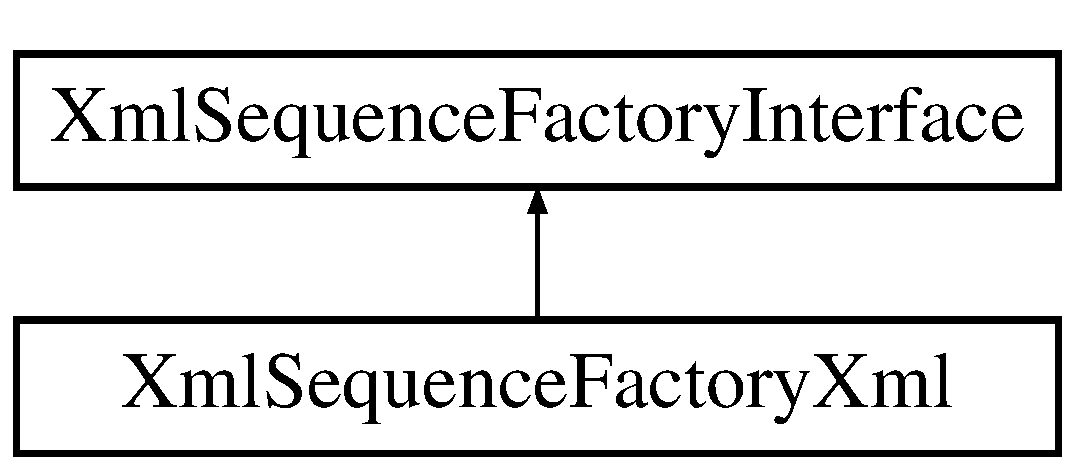
\includegraphics[height=2cm]{interface_xml_sequence_factory_interface}
\end{center}
\end{figure}
\subsection*{Public Member Functions}
\begin{CompactItemize}
\item 
\hyperlink{interface_xml_sequence_factory_interface_8fbb97bc3fbf487c357f5a255a3a2357}{setXmlSequence} (\hyperlink{class_xml_sequence}{XmlSequence} \$objXmlSequence)
\item 
\hyperlink{interface_xml_sequence_factory_interface_a6f31a5f6a768055644ddb62d101cbb6}{getXmlSequence} ()
\item 
\hyperlink{interface_xml_sequence_factory_interface_c06f18d6c688317b41477c315f7008f7}{perform} ()
\end{CompactItemize}
\subsection*{Static Public Member Functions}
\begin{CompactItemize}
\item 
static \hyperlink{interface_xml_sequence_factory_interface_5ad765cdd7548f50459910554b46b015}{getInstance} ()
\end{CompactItemize}


\subsection{Member Function Documentation}
\hypertarget{interface_xml_sequence_factory_interface_5ad765cdd7548f50459910554b46b015}{
\index{XmlSequenceFactoryInterface@{XmlSequenceFactoryInterface}!getInstance@{getInstance}}
\index{getInstance@{getInstance}!XmlSequenceFactoryInterface@{XmlSequenceFactoryInterface}}
\subsubsection[{getInstance}]{\setlength{\rightskip}{0pt plus 5cm}static XmlSequenceFactoryInterface::getInstance ()\hspace{0.3cm}{\tt  \mbox{[}static\mbox{]}}}}
\label{interface_xml_sequence_factory_interface_5ad765cdd7548f50459910554b46b015}


Return the singleton of the \hyperlink{interface_xml_sequence_factory_interface}{XmlSequenceFactoryInterface}

\begin{Desc}
\item[Returns:]\hyperlink{interface_xml_sequence_factory_interface}{XmlSequenceFactoryInterface} \end{Desc}


Implemented in \hyperlink{class_xml_sequence_factory_xml_04cfad5bd111c3dd8f264e783ed91328}{XmlSequenceFactoryXml}.\hypertarget{interface_xml_sequence_factory_interface_a6f31a5f6a768055644ddb62d101cbb6}{
\index{XmlSequenceFactoryInterface@{XmlSequenceFactoryInterface}!getXmlSequence@{getXmlSequence}}
\index{getXmlSequence@{getXmlSequence}!XmlSequenceFactoryInterface@{XmlSequenceFactoryInterface}}
\subsubsection[{getXmlSequence}]{\setlength{\rightskip}{0pt plus 5cm}XmlSequenceFactoryInterface::getXmlSequence ()}}
\label{interface_xml_sequence_factory_interface_a6f31a5f6a768055644ddb62d101cbb6}


get the xml sequence object

\begin{Desc}
\item[See also:]XmlSequenceFactoryInterface-$>$\hyperlink{interface_xml_sequence_factory_interface_a6f31a5f6a768055644ddb62d101cbb6}{getXmlSequence()} \end{Desc}
\begin{Desc}
\item[Returns:]\hyperlink{class_xml_sequence}{XmlSequence} \end{Desc}


Implemented in \hyperlink{class_xml_sequence_factory_xml_fba8de983895bb05857d75f9b26dd71a}{XmlSequenceFactoryXml}.\hypertarget{interface_xml_sequence_factory_interface_c06f18d6c688317b41477c315f7008f7}{
\index{XmlSequenceFactoryInterface@{XmlSequenceFactoryInterface}!perform@{perform}}
\index{perform@{perform}!XmlSequenceFactoryInterface@{XmlSequenceFactoryInterface}}
\subsubsection[{perform}]{\setlength{\rightskip}{0pt plus 5cm}XmlSequenceFactoryInterface::perform ()}}
\label{interface_xml_sequence_factory_interface_c06f18d6c688317b41477c315f7008f7}


create a xml sequence based into its configurations

\begin{Desc}
\item[See also:]XmlSequenceFactoryInterface-$>$\hyperlink{interface_xml_sequence_factory_interface_c06f18d6c688317b41477c315f7008f7}{perform()} \end{Desc}
\begin{Desc}
\item[Returns:]\hyperlink{class_xml_sequence}{XmlSequence} \end{Desc}


Implemented in \hyperlink{class_xml_sequence_factory_xml_f9deb0d1efc6f6e726837251a5759bcc}{XmlSequenceFactoryXml}.\hypertarget{interface_xml_sequence_factory_interface_8fbb97bc3fbf487c357f5a255a3a2357}{
\index{XmlSequenceFactoryInterface@{XmlSequenceFactoryInterface}!setXmlSequence@{setXmlSequence}}
\index{setXmlSequence@{setXmlSequence}!XmlSequenceFactoryInterface@{XmlSequenceFactoryInterface}}
\subsubsection[{setXmlSequence}]{\setlength{\rightskip}{0pt plus 5cm}XmlSequenceFactoryInterface::setXmlSequence ({\bf XmlSequence} \$ {\em objXmlSequence})}}
\label{interface_xml_sequence_factory_interface_8fbb97bc3fbf487c357f5a255a3a2357}


set the xml sequence object

\begin{Desc}
\item[See also:]XmlSequenceFactoryInterface-$>$setXmlSequence( XmlSequence ) \end{Desc}
\begin{Desc}
\item[Parameters:]
\begin{description}
\item[{\em \$objXmlSequence}]\end{description}
\end{Desc}
\begin{Desc}
\item[Returns:]\hyperlink{interface_xml_sequence_factory_interface}{XmlSequenceFactoryInterface} \end{Desc}


Implemented in \hyperlink{class_xml_sequence_factory_xml_c1282bb7211c84aff732419317312152}{XmlSequenceFactoryXml}.

The documentation for this interface was generated from the following file:\begin{CompactItemize}
\item 
components/xmlSequence/\hyperlink{_xml_sequence_factory_interface_8interface_8php}{XmlSequenceFactoryInterface.interface.php}\end{CompactItemize}

\hypertarget{class_xml_sequence_factory_xml}{
\section{XmlSequenceFactoryXml Class Reference}
\label{class_xml_sequence_factory_xml}\index{XmlSequenceFactoryXml@{XmlSequenceFactoryXml}}
}
Inheritance diagram for XmlSequenceFactoryXml::\begin{figure}[H]
\begin{center}
\leavevmode
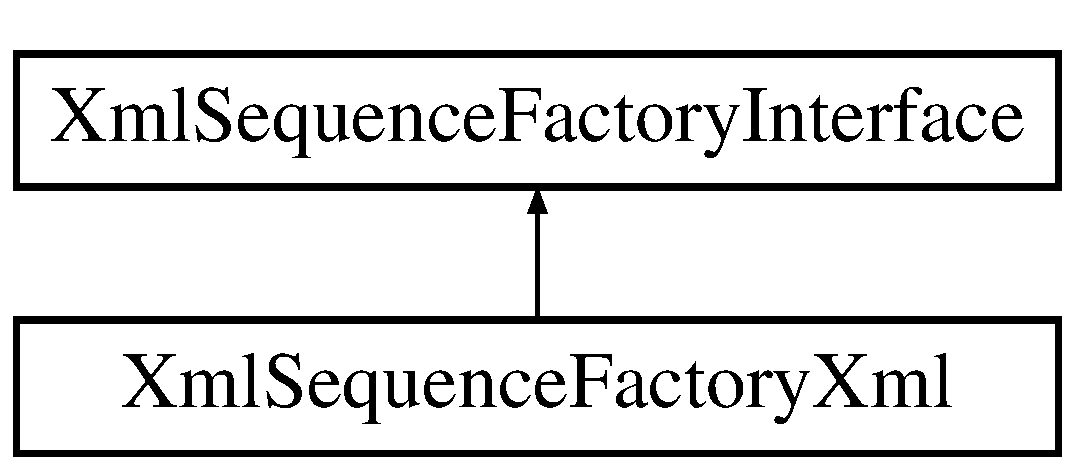
\includegraphics[height=2cm]{class_xml_sequence_factory_xml}
\end{center}
\end{figure}
\subsection*{Public Member Functions}
\begin{CompactItemize}
\item 
\hyperlink{class_xml_sequence_factory_xml_8ac34bd040fb3627c7b4ca12808d427f}{setXml} (\$strXml)
\item 
\hyperlink{class_xml_sequence_factory_xml_1ff0576538bf186559839cada0449ddf}{getXml} ()
\item 
\hyperlink{class_xml_sequence_factory_xml_65967fe6cc76b0c0b28aa39e9acffcab}{setXmlSequence} (\hyperlink{class_xml_sequence}{XmlSequence} \$objXmlSequence)
\item 
\hyperlink{class_xml_sequence_factory_xml_feb0ab0d5955fcae20ff5062fa59fd79}{getXmlSequence} ()
\item 
\hyperlink{class_xml_sequence_factory_xml_469121070b5e6118f202517380558019}{perform} ()
\end{CompactItemize}
\subsection*{Static Public Member Functions}
\begin{CompactItemize}
\item 
static \hyperlink{class_xml_sequence_factory_xml_c93fbec81f07e5d15f80db907e63dc10}{getInstance} ()
\end{CompactItemize}
\subsection*{Protected Member Functions}
\begin{CompactItemize}
\item 
\hyperlink{class_xml_sequence_factory_xml_390c089130460866b440b2f6f73dd136}{loadActors} ()
\item 
\hyperlink{class_xml_sequence_factory_xml_589f548f18802f9a10d0eaca5cab970c}{loadMessages} ()
\end{CompactItemize}
\subsection*{Protected Attributes}
\begin{CompactItemize}
\item 
\hyperlink{class_xml_sequence_factory_xml_eefa469c1b13fe1fec040c910b720034}{\$objXmlSequence}
\item 
\hyperlink{class_xml_sequence_factory_xml_bc4e6de2df0815964fa9983816b76475}{\$objXml}
\end{CompactItemize}
\subsection*{Static Protected Attributes}
\begin{CompactItemize}
\item 
static \hyperlink{class_xml_sequence_factory_xml_917d057900327b25608ed26c927eac3b}{\$objInstance}
\end{CompactItemize}


\subsection{Detailed Description}
Factory what creates \hyperlink{class_xml_sequence}{XmlSequence} based into Xml Files \begin{Desc}
\item[Author:]Thiago Henrique Ramos da Mata $<$\href{mailto:thiago.henrique.mata@gmail.com}{\tt thiago.henrique.mata@gmail.com}$>$ \end{Desc}


\subsection{Member Function Documentation}
\hypertarget{class_xml_sequence_factory_xml_c93fbec81f07e5d15f80db907e63dc10}{
\index{XmlSequenceFactoryXml@{XmlSequenceFactoryXml}!getInstance@{getInstance}}
\index{getInstance@{getInstance}!XmlSequenceFactoryXml@{XmlSequenceFactoryXml}}
\subsubsection[{getInstance}]{\setlength{\rightskip}{0pt plus 5cm}static getInstance ()\hspace{0.3cm}{\tt  \mbox{[}static\mbox{]}}}}
\label{class_xml_sequence_factory_xml_c93fbec81f07e5d15f80db907e63dc10}


Return the singleton of the \hyperlink{class_xml_sequence_factory_xml}{XmlSequenceFactoryXml}

\begin{Desc}
\item[Returns:]\hyperlink{class_xml_sequence_factory_xml}{XmlSequenceFactoryXml} \end{Desc}


Implements \hyperlink{interface_xml_sequence_factory_interface_c93fbec81f07e5d15f80db907e63dc10}{XmlSequenceFactoryInterface}.

\begin{Code}\begin{verbatim}42         {
43                 if( self::$objInstance == null )
44                 {
45                         self::$objInstance = new XmlSequenceFactoryXml();
46                 }
47                 return self::$objInstance;
48         }               
\end{verbatim}
\end{Code}


\hypertarget{class_xml_sequence_factory_xml_1ff0576538bf186559839cada0449ddf}{
\index{XmlSequenceFactoryXml@{XmlSequenceFactoryXml}!getXml@{getXml}}
\index{getXml@{getXml}!XmlSequenceFactoryXml@{XmlSequenceFactoryXml}}
\subsubsection[{getXml}]{\setlength{\rightskip}{0pt plus 5cm}getXml ()}}
\label{class_xml_sequence_factory_xml_1ff0576538bf186559839cada0449ddf}


Get the xml of the sequence object

\begin{Desc}
\item[See also:]XmlSequence-$>$objXml 

XmlSequence::setXml( string ) \end{Desc}
\begin{Desc}
\item[Parameters:]
\begin{description}
\item[{\em string}]\$strXml \end{description}
\end{Desc}
\begin{Desc}
\item[Returns:]SimpleXmlElement \end{Desc}


\begin{Code}\begin{verbatim}74     {
75         return $this->objXml;
76     }
\end{verbatim}
\end{Code}


\hypertarget{class_xml_sequence_factory_xml_feb0ab0d5955fcae20ff5062fa59fd79}{
\index{XmlSequenceFactoryXml@{XmlSequenceFactoryXml}!getXmlSequence@{getXmlSequence}}
\index{getXmlSequence@{getXmlSequence}!XmlSequenceFactoryXml@{XmlSequenceFactoryXml}}
\subsubsection[{getXmlSequence}]{\setlength{\rightskip}{0pt plus 5cm}getXmlSequence ()}}
\label{class_xml_sequence_factory_xml_feb0ab0d5955fcae20ff5062fa59fd79}


get the xml sequence object

\begin{Desc}
\item[See also:]XmlSequenceFactoryInterface-$>$\hyperlink{class_xml_sequence_factory_xml_feb0ab0d5955fcae20ff5062fa59fd79}{getXmlSequence()} \end{Desc}
\begin{Desc}
\item[Returns:]\hyperlink{class_xml_sequence}{XmlSequence} \end{Desc}


Implements \hyperlink{interface_xml_sequence_factory_interface_feb0ab0d5955fcae20ff5062fa59fd79}{XmlSequenceFactoryInterface}.

\begin{Code}\begin{verbatim}98     {
99         return $this->objXmlSequence;   
100     }
\end{verbatim}
\end{Code}


\hypertarget{class_xml_sequence_factory_xml_390c089130460866b440b2f6f73dd136}{
\index{XmlSequenceFactoryXml@{XmlSequenceFactoryXml}!loadActors@{loadActors}}
\index{loadActors@{loadActors}!XmlSequenceFactoryXml@{XmlSequenceFactoryXml}}
\subsubsection[{loadActors}]{\setlength{\rightskip}{0pt plus 5cm}loadActors ()\hspace{0.3cm}{\tt  \mbox{[}protected\mbox{]}}}}
\label{class_xml_sequence_factory_xml_390c089130460866b440b2f6f73dd136}


Load the xml file and based on it insert a list of actors into the \hyperlink{class_xml_sequence}{XmlSequence} Object 

\begin{Code}\begin{verbatim}121     {
122         $arrActors = $this->getXmlSequence()->getActors();
123         
124         foreach( $this->objXml->actors->actor as $xmlActor )
125         {
126             $intId = (integer)$xmlActor['id'];
127             $strType = (string)$xmlActor['type'];
128             $strName = (string)$xmlActor;
129 
130             $objActor = new XmlSequenceActor();
131             $objActor->setId( $intId );
132             $objActor->setType( $strType );
133             $objActor->setName( $strName );
134 
135             $arrActors[ $objActor->getId() ] = $objActor;
136         }
137         ksort( $arrActors );
138         $this->getXmlSequence()->setActors( $arrActors );
139     }
\end{verbatim}
\end{Code}


\hypertarget{class_xml_sequence_factory_xml_589f548f18802f9a10d0eaca5cab970c}{
\index{XmlSequenceFactoryXml@{XmlSequenceFactoryXml}!loadMessages@{loadMessages}}
\index{loadMessages@{loadMessages}!XmlSequenceFactoryXml@{XmlSequenceFactoryXml}}
\subsubsection[{loadMessages}]{\setlength{\rightskip}{0pt plus 5cm}loadMessages ()\hspace{0.3cm}{\tt  \mbox{[}protected\mbox{]}}}}
\label{class_xml_sequence_factory_xml_589f548f18802f9a10d0eaca5cab970c}


Load the xml file and based on it insert a list of messages into the \hyperlink{class_xml_sequence}{XmlSequence} Object 

\begin{Code}\begin{verbatim}146     {
147         $arrMessages = $this->getXmlSequence()->getMessages();
148         $arrActors = $this->getXmlSequence()->getActors();
149         
150         foreach( $this->objXml->messages->message as $xmlMessage )
151         {
152             $intFrom    = (integer)$xmlMessage[ 'from' ];
153             $intTo      = (integer)$xmlMessage[ 'to' ];
154             $strType    = (string) $xmlMessage[ 'type' ];
155             $strText = (string) $xmlMessage[ 'text' ];
156 
157             $objMessage = new XmlSequenceMessage();
158             $objMessage->setType( $strType );
159             $objMessage->setText( $strText );
160 
161            if( !array_key_exists( $intFrom , $arrActors ) )
162             {
163                 throw new Exception( ' Actor From ' . $intFrom . ' not Found ' );
164             }
165             $objMessage->setActorFrom( $arrActors[ $intFrom ] );
166 
167            if( !array_key_exists( $intTo , $arrActors ) )
168             {
169                 throw new Exception( ' Actor To ' . $intTo . ' not Found ' );
170             }
171             $objMessage->setActorTo( $arrActors[ $intTo ] );
172 
173             if( isset( $xmlMessage->values->value ) )
174             foreach( $xmlMessage->values->value as $xmlValue )
175             {
176                 $strName = (string)$xmlValue['name'];
177                 $strValue = (string)$xmlValue['value'];
178                 $objValue = new XmlSequenceValue();
179                 $objValue->setName( $strName );
180                 $objValue->setValue( $strValue );
181 
182                 $objMessage->addValue( $objValue );
183             }
184 
185             $arrMessages[] = $objMessage;
186         }
187         $this->getXmlSequence()->setMessages( $arrMessages );
188     }
\end{verbatim}
\end{Code}


\hypertarget{class_xml_sequence_factory_xml_469121070b5e6118f202517380558019}{
\index{XmlSequenceFactoryXml@{XmlSequenceFactoryXml}!perform@{perform}}
\index{perform@{perform}!XmlSequenceFactoryXml@{XmlSequenceFactoryXml}}
\subsubsection[{perform}]{\setlength{\rightskip}{0pt plus 5cm}perform ()}}
\label{class_xml_sequence_factory_xml_469121070b5e6118f202517380558019}


create a xml sequence based into its configurations

\begin{Desc}
\item[See also:]XmlSequenceFactoryInterface-$>$\hyperlink{class_xml_sequence_factory_xml_469121070b5e6118f202517380558019}{perform()} \end{Desc}
\begin{Desc}
\item[Returns:]\hyperlink{class_xml_sequence}{XmlSequence} \end{Desc}


Implements \hyperlink{interface_xml_sequence_factory_interface_469121070b5e6118f202517380558019}{XmlSequenceFactoryInterface}.

\begin{Code}\begin{verbatim}109     {
110         $this->setXmlSequence( new XmlSequence() );
111         $this->loadActors();
112         $this->loadMessages();
113         return $this->getXmlSequence();
114     }
\end{verbatim}
\end{Code}


\hypertarget{class_xml_sequence_factory_xml_8ac34bd040fb3627c7b4ca12808d427f}{
\index{XmlSequenceFactoryXml@{XmlSequenceFactoryXml}!setXml@{setXml}}
\index{setXml@{setXml}!XmlSequenceFactoryXml@{XmlSequenceFactoryXml}}
\subsubsection[{setXml}]{\setlength{\rightskip}{0pt plus 5cm}setXml (\$ {\em strXml})}}
\label{class_xml_sequence_factory_xml_8ac34bd040fb3627c7b4ca12808d427f}


Set the xml of the sequence object

\begin{Desc}
\item[See also:]XmlSequence-$>$objXml 

XmlSequence::getXml() \end{Desc}
\begin{Desc}
\item[Parameters:]
\begin{description}
\item[{\em string}]\$strXml \end{description}
\end{Desc}
\begin{Desc}
\item[Returns:]\hyperlink{class_xml_sequence_factory_xml}{XmlSequenceFactoryXml} me \end{Desc}


\begin{Code}\begin{verbatim}60     {
61         $this->objXml = simplexml_load_string( $strXml );
62         return $this;
63     }
\end{verbatim}
\end{Code}


\hypertarget{class_xml_sequence_factory_xml_65967fe6cc76b0c0b28aa39e9acffcab}{
\index{XmlSequenceFactoryXml@{XmlSequenceFactoryXml}!setXmlSequence@{setXmlSequence}}
\index{setXmlSequence@{setXmlSequence}!XmlSequenceFactoryXml@{XmlSequenceFactoryXml}}
\subsubsection[{setXmlSequence}]{\setlength{\rightskip}{0pt plus 5cm}setXmlSequence ({\bf XmlSequence} \$ {\em objXmlSequence})}}
\label{class_xml_sequence_factory_xml_65967fe6cc76b0c0b28aa39e9acffcab}


set the xml sequence object

\begin{Desc}
\item[See also:]XmlSequenceFactoryInterface-$>$setXmlSequence( XmlSequence ) \end{Desc}
\begin{Desc}
\item[Parameters:]
\begin{description}
\item[{\em \$objXmlSequence}]\end{description}
\end{Desc}
\begin{Desc}
\item[Returns:]\hyperlink{class_xml_sequence_factory_xml}{XmlSequenceFactoryXml} me \end{Desc}


Implements \hyperlink{interface_xml_sequence_factory_interface_65967fe6cc76b0c0b28aa39e9acffcab}{XmlSequenceFactoryInterface}.

\begin{Code}\begin{verbatim}86     {
87         $this->objXmlSequence = $objXmlSequence;        
88         return $this;
89     }
\end{verbatim}
\end{Code}




\subsection{Member Data Documentation}
\hypertarget{class_xml_sequence_factory_xml_917d057900327b25608ed26c927eac3b}{
\index{XmlSequenceFactoryXml@{XmlSequenceFactoryXml}!\$objInstance@{\$objInstance}}
\index{\$objInstance@{\$objInstance}!XmlSequenceFactoryXml@{XmlSequenceFactoryXml}}
\subsubsection[{\$objInstance}]{\setlength{\rightskip}{0pt plus 5cm}\$objInstance\hspace{0.3cm}{\tt  \mbox{[}static, protected\mbox{]}}}}
\label{class_xml_sequence_factory_xml_917d057900327b25608ed26c927eac3b}


Singleton of the \hyperlink{class_xml_sequence_factory_xml}{XmlSequenceFactoryXml}

\begin{Desc}
\item[See also:]XmlSequenceFactoryInterface::\$objInstance\end{Desc}
\hyperlink{class_xml_sequence_factory_xml}{XmlSequenceFactoryXml} \hypertarget{class_xml_sequence_factory_xml_bc4e6de2df0815964fa9983816b76475}{
\index{XmlSequenceFactoryXml@{XmlSequenceFactoryXml}!\$objXml@{\$objXml}}
\index{\$objXml@{\$objXml}!XmlSequenceFactoryXml@{XmlSequenceFactoryXml}}
\subsubsection[{\$objXml}]{\setlength{\rightskip}{0pt plus 5cm}\$objXml\hspace{0.3cm}{\tt  \mbox{[}protected\mbox{]}}}}
\label{class_xml_sequence_factory_xml_bc4e6de2df0815964fa9983816b76475}


Simple Xml element used to access information from a xml

SimpleXmlElement \hypertarget{class_xml_sequence_factory_xml_eefa469c1b13fe1fec040c910b720034}{
\index{XmlSequenceFactoryXml@{XmlSequenceFactoryXml}!\$objXmlSequence@{\$objXmlSequence}}
\index{\$objXmlSequence@{\$objXmlSequence}!XmlSequenceFactoryXml@{XmlSequenceFactoryXml}}
\subsubsection[{\$objXmlSequence}]{\setlength{\rightskip}{0pt plus 5cm}\$objXmlSequence\hspace{0.3cm}{\tt  \mbox{[}protected\mbox{]}}}}
\label{class_xml_sequence_factory_xml_eefa469c1b13fe1fec040c910b720034}


Xml Sequence Object in factory

\begin{Desc}
\item[See also:]XmlSequenceFactoryInterface-$>$objXmlSequence\end{Desc}
\hyperlink{class_xml_sequence}{XmlSequence} 

The documentation for this class was generated from the following file:\begin{CompactItemize}
\item 
components/xmlSequence/\hyperlink{_xml_sequence_factory_xml_8class_8php}{XmlSequenceFactoryXml.class.php}\end{CompactItemize}

\hypertarget{class_xml_sequence_message}{
\section{XmlSequenceMessage Class Reference}
\label{class_xml_sequence_message}\index{XmlSequenceMessage@{XmlSequenceMessage}}
}
\subsection*{Public Member Functions}
\begin{CompactItemize}
\item 
\hyperlink{class_xml_sequence_message_a4d5880601982b4e882e52f657480cc5}{setText} (\$strText)
\item 
\hyperlink{class_xml_sequence_message_1f80c7d126fc2183c3c99a71df3f1d20}{getText} ()
\item 
\hyperlink{class_xml_sequence_message_a6a08c247856f2721b867676aa130214}{setType} (\$strType)
\item 
\hyperlink{class_xml_sequence_message_d839c7bfe476a42ddf264d019a13938b}{getType} ()
\item 
\hyperlink{class_xml_sequence_message_8dd8205552a1f91a32541187ff799d2f}{setActorFrom} (\hyperlink{class_xml_sequence_actor}{XmlSequenceActor} \$objActor)
\item 
\hyperlink{class_xml_sequence_message_d174306473bc3ba17083bd0c2c100443}{getActorFrom} ()
\item 
\hyperlink{class_xml_sequence_message_dd5dde3ef38d814ef76f6855b38cebc8}{setActorTo} (\hyperlink{class_xml_sequence_actor}{XmlSequenceActor} \$objActor)
\item 
\hyperlink{class_xml_sequence_message_d67a02882cb2602e3171f012650160f6}{getActorTo} ()
\item 
\hyperlink{class_xml_sequence_message_4ed3a9eceec6ce84566098813fde6101}{setValues} (Array \$arrValues)
\item 
\hyperlink{class_xml_sequence_message_9c2e8f8d995477aad79640ad673ab6a9}{getValues} ()
\item 
\hyperlink{class_xml_sequence_message_fc28193031e8ccdedf401767f7881267}{addValue} (\hyperlink{class_xml_sequence_value}{XmlSequenceValue} \$objValue)
\item 
\hyperlink{class_xml_sequence_message_4125b914cfa073d64b144b5607efdb3d}{setTimeStart} (\$intTime)
\item 
\hyperlink{class_xml_sequence_message_27b24a732d56e0b1cf7fd755d2c52983}{getTimeStart} ()
\item 
\hyperlink{class_xml_sequence_message_7fddd3ce13210832ec0ec73a751c332c}{setTimeEnd} (\$intTime)
\item 
\hyperlink{class_xml_sequence_message_a0c32ce53d9ecdff7099c221126fb58c}{getTimeEnd} ()
\item 
\hyperlink{class_xml_sequence_message_0f7538c36a98475fcd35cd554e7c7d05}{getTimeDuration} ()
\item 
\hyperlink{class_xml_sequence_message_c73e3d276fb5b60bfac84c7bda29cb1e}{isReverse} ()
\item 
\hyperlink{class_xml_sequence_message_c2fdfe0fd692c08d72faf1ca63fb7263}{isLarge} ()
\item 
\hyperlink{class_xml_sequence_message_50dd7454dfc6418b76613e6518a1fcc1}{isRecursive} ()
\end{CompactItemize}
\subsection*{Protected Attributes}
\begin{CompactItemize}
\item 
\hyperlink{class_xml_sequence_message_5191806ce342246e9febbb7188ef914f}{\$strText} = null
\item 
\hyperlink{class_xml_sequence_message_9cbf41c891bfaaacc0048ec4e7f54765}{\$strType} = null
\item 
\hyperlink{class_xml_sequence_message_677eb4ecb7493d72f3ea96d6b896f5c4}{\$objActorFrom} = null
\item 
\hyperlink{class_xml_sequence_message_6e35efb1112d87db5a90f660f2c7e487}{\$objActorTo} = null
\item 
\hyperlink{class_xml_sequence_message_97999a3267c23300fddf5d7e0ff0e87d}{\$arrValues} = Array()
\item 
\hyperlink{class_xml_sequence_message_3e60774808cf2fd2fe04898ca6314184}{\$intTimeStart}
\item 
\hyperlink{class_xml_sequence_message_5c82454b9be08a7fc94fd580932f59c1}{\$intTimeEnd}
\end{CompactItemize}


\subsection{Member Function Documentation}
\hypertarget{class_xml_sequence_message_fc28193031e8ccdedf401767f7881267}{
\index{XmlSequenceMessage@{XmlSequenceMessage}!addValue@{addValue}}
\index{addValue@{addValue}!XmlSequenceMessage@{XmlSequenceMessage}}
\subsubsection[{addValue}]{\setlength{\rightskip}{0pt plus 5cm}XmlSequenceMessage::addValue ({\bf XmlSequenceValue} \$ {\em objValue})}}
\label{class_xml_sequence_message_fc28193031e8ccdedf401767f7881267}


Append one \hyperlink{class_xml_sequence_value}{XmlSequenceValue} into the collection of Values of the message

\begin{Desc}
\item[See also:]\hyperlink{class_xml_sequence_message_4ed3a9eceec6ce84566098813fde6101}{XmlSequenceMessage::setValues}( \hyperlink{class_xml_sequence_value}{XmlSequenceValue}\mbox{[}\mbox{]} ) 

XmlSequenceMessage-$>$arrValues 

\hyperlink{class_xml_sequence_message_9c2e8f8d995477aad79640ad673ab6a9}{XmlSequenceMessage::getValues()} 

\hyperlink{class_xml_sequence_value}{XmlSequenceValue} \end{Desc}
\begin{Desc}
\item[Parameters:]
\begin{description}
\item[{\em \hyperlink{class_xml_sequence_value}{XmlSequenceValue}}]\$objValue \end{description}
\end{Desc}
\hypertarget{class_xml_sequence_message_d174306473bc3ba17083bd0c2c100443}{
\index{XmlSequenceMessage@{XmlSequenceMessage}!getActorFrom@{getActorFrom}}
\index{getActorFrom@{getActorFrom}!XmlSequenceMessage@{XmlSequenceMessage}}
\subsubsection[{getActorFrom}]{\setlength{\rightskip}{0pt plus 5cm}XmlSequenceMessage::getActorFrom ()}}
\label{class_xml_sequence_message_d174306473bc3ba17083bd0c2c100443}


Returns the actor who is the recipient of the message

\begin{Desc}
\item[See also:]XmlSequenceMessage::setActorFrom( XmlSequenceActor ) 

XmlSequenceMessage-$>$objActorFrom 

\hyperlink{class_xml_sequence_actor}{XmlSequenceActor} \end{Desc}
\begin{Desc}
\item[Returns:]\hyperlink{class_xml_sequence_actor}{XmlSequenceActor} \end{Desc}
\hypertarget{class_xml_sequence_message_d67a02882cb2602e3171f012650160f6}{
\index{XmlSequenceMessage@{XmlSequenceMessage}!getActorTo@{getActorTo}}
\index{getActorTo@{getActorTo}!XmlSequenceMessage@{XmlSequenceMessage}}
\subsubsection[{getActorTo}]{\setlength{\rightskip}{0pt plus 5cm}XmlSequenceMessage::getActorTo ()}}
\label{class_xml_sequence_message_d67a02882cb2602e3171f012650160f6}


Returns the actor who is the author of the message

\begin{Desc}
\item[See also:]XmlSequenceMessage::setActorTo( XmlSequenceActor ) 

XmlSequenceMessage-$>$objActorTo 

\hyperlink{class_xml_sequence_actor}{XmlSequenceActor} \end{Desc}
\begin{Desc}
\item[Returns:]\hyperlink{class_xml_sequence_actor}{XmlSequenceActor} \end{Desc}
\hypertarget{class_xml_sequence_message_1f80c7d126fc2183c3c99a71df3f1d20}{
\index{XmlSequenceMessage@{XmlSequenceMessage}!getText@{getText}}
\index{getText@{getText}!XmlSequenceMessage@{XmlSequenceMessage}}
\subsubsection[{getText}]{\setlength{\rightskip}{0pt plus 5cm}XmlSequenceMessage::getText ()}}
\label{class_xml_sequence_message_1f80c7d126fc2183c3c99a71df3f1d20}


Get the text of the message

\begin{Desc}
\item[See also:]XmlSequenceMessage::setText( string ) 

XmlSequenceMessage-$>$strText \end{Desc}
\begin{Desc}
\item[Returns:]string \end{Desc}
\hypertarget{class_xml_sequence_message_0f7538c36a98475fcd35cd554e7c7d05}{
\index{XmlSequenceMessage@{XmlSequenceMessage}!getTimeDuration@{getTimeDuration}}
\index{getTimeDuration@{getTimeDuration}!XmlSequenceMessage@{XmlSequenceMessage}}
\subsubsection[{getTimeDuration}]{\setlength{\rightskip}{0pt plus 5cm}XmlSequenceMessage::getTimeDuration ()}}
\label{class_xml_sequence_message_0f7538c36a98475fcd35cd554e7c7d05}


Return the duration in timestamp betwenn the start end end of the message

\begin{Desc}
\item[Returns:]integer \end{Desc}
\hypertarget{class_xml_sequence_message_a0c32ce53d9ecdff7099c221126fb58c}{
\index{XmlSequenceMessage@{XmlSequenceMessage}!getTimeEnd@{getTimeEnd}}
\index{getTimeEnd@{getTimeEnd}!XmlSequenceMessage@{XmlSequenceMessage}}
\subsubsection[{getTimeEnd}]{\setlength{\rightskip}{0pt plus 5cm}XmlSequenceMessage::getTimeEnd ()}}
\label{class_xml_sequence_message_a0c32ce53d9ecdff7099c221126fb58c}


Get the timestamp when the message ends

\begin{Desc}
\item[See also:]XmlSequenceMessage-$>$intTimeEnd 

XmlSequenceMessage::setTimeEnd( integer ) \end{Desc}
\begin{Desc}
\item[Returns:]integer \end{Desc}
\hypertarget{class_xml_sequence_message_27b24a732d56e0b1cf7fd755d2c52983}{
\index{XmlSequenceMessage@{XmlSequenceMessage}!getTimeStart@{getTimeStart}}
\index{getTimeStart@{getTimeStart}!XmlSequenceMessage@{XmlSequenceMessage}}
\subsubsection[{getTimeStart}]{\setlength{\rightskip}{0pt plus 5cm}XmlSequenceMessage::getTimeStart ()}}
\label{class_xml_sequence_message_27b24a732d56e0b1cf7fd755d2c52983}


Get the timestamp when the message started

\begin{Desc}
\item[See also:]XmlSequenceMessage-$>$intTimeStart 

XmlSequenceMessage::setTimeStart( integer ) \end{Desc}
\begin{Desc}
\item[Returns:]integer \end{Desc}
\hypertarget{class_xml_sequence_message_d839c7bfe476a42ddf264d019a13938b}{
\index{XmlSequenceMessage@{XmlSequenceMessage}!getType@{getType}}
\index{getType@{getType}!XmlSequenceMessage@{XmlSequenceMessage}}
\subsubsection[{getType}]{\setlength{\rightskip}{0pt plus 5cm}XmlSequenceMessage::getType ()}}
\label{class_xml_sequence_message_d839c7bfe476a42ddf264d019a13938b}


Get the type of the message

\begin{Desc}
\item[See also:]XmlSequenceMessage::setType( string ) 

XmlSequenceMessage-$>$strType \end{Desc}
\begin{Desc}
\item[Returns:]string \end{Desc}
\hypertarget{class_xml_sequence_message_9c2e8f8d995477aad79640ad673ab6a9}{
\index{XmlSequenceMessage@{XmlSequenceMessage}!getValues@{getValues}}
\index{getValues@{getValues}!XmlSequenceMessage@{XmlSequenceMessage}}
\subsubsection[{getValues}]{\setlength{\rightskip}{0pt plus 5cm}XmlSequenceMessage::getValues ()}}
\label{class_xml_sequence_message_9c2e8f8d995477aad79640ad673ab6a9}


Get the array of values of the message

\begin{Desc}
\item[See also:]\hyperlink{class_xml_sequence_message_4ed3a9eceec6ce84566098813fde6101}{XmlSequenceMessage::setValues}( \hyperlink{class_xml_sequence_value}{XmlSequenceValue}\mbox{[}\mbox{]} ) 

XmlSequenceMessage-$>$arrValues 

\hyperlink{class_xml_sequence_value}{XmlSequenceValue} \end{Desc}
\begin{Desc}
\item[Returns:]\hyperlink{class_xml_sequence_value}{XmlSequenceValue}\mbox{[}\mbox{]} \end{Desc}
\hypertarget{class_xml_sequence_message_c2fdfe0fd692c08d72faf1ca63fb7263}{
\index{XmlSequenceMessage@{XmlSequenceMessage}!isLarge@{isLarge}}
\index{isLarge@{isLarge}!XmlSequenceMessage@{XmlSequenceMessage}}
\subsubsection[{isLarge}]{\setlength{\rightskip}{0pt plus 5cm}XmlSequenceMessage::isLarge ()}}
\label{class_xml_sequence_message_c2fdfe0fd692c08d72faf1ca63fb7263}


Returns {\tt true} if the distance between the actor from and the actor to be bigger then 1, {\tt false} otherwise

\begin{Desc}
\item[Returns:]boolean \end{Desc}
\hypertarget{class_xml_sequence_message_50dd7454dfc6418b76613e6518a1fcc1}{
\index{XmlSequenceMessage@{XmlSequenceMessage}!isRecursive@{isRecursive}}
\index{isRecursive@{isRecursive}!XmlSequenceMessage@{XmlSequenceMessage}}
\subsubsection[{isRecursive}]{\setlength{\rightskip}{0pt plus 5cm}XmlSequenceMessage::isRecursive ()}}
\label{class_xml_sequence_message_50dd7454dfc6418b76613e6518a1fcc1}


Returns {\tt true} if the actor from it is the actor to, {\tt false} otherwise

\begin{Desc}
\item[Returns:]boolean \end{Desc}
\hypertarget{class_xml_sequence_message_c73e3d276fb5b60bfac84c7bda29cb1e}{
\index{XmlSequenceMessage@{XmlSequenceMessage}!isReverse@{isReverse}}
\index{isReverse@{isReverse}!XmlSequenceMessage@{XmlSequenceMessage}}
\subsubsection[{isReverse}]{\setlength{\rightskip}{0pt plus 5cm}XmlSequenceMessage::isReverse ()}}
\label{class_xml_sequence_message_c73e3d276fb5b60bfac84c7bda29cb1e}


Returns {\tt true} if the id of the actor from is bigger then the id of the actor to, {\tt false} otherwise

\begin{Desc}
\item[Returns:]boolean \end{Desc}
\hypertarget{class_xml_sequence_message_8dd8205552a1f91a32541187ff799d2f}{
\index{XmlSequenceMessage@{XmlSequenceMessage}!setActorFrom@{setActorFrom}}
\index{setActorFrom@{setActorFrom}!XmlSequenceMessage@{XmlSequenceMessage}}
\subsubsection[{setActorFrom}]{\setlength{\rightskip}{0pt plus 5cm}XmlSequenceMessage::setActorFrom ({\bf XmlSequenceActor} \$ {\em objActor})}}
\label{class_xml_sequence_message_8dd8205552a1f91a32541187ff799d2f}


Inform the actor who is the recipient of the message

\begin{Desc}
\item[See also:]\hyperlink{class_xml_sequence_message_d174306473bc3ba17083bd0c2c100443}{XmlSequenceMessage::getActorFrom()} 

XmlSequenceMessage-$>$objActorFrom 

\hyperlink{class_xml_sequence_actor}{XmlSequenceActor} \end{Desc}
\begin{Desc}
\item[Parameters:]
\begin{description}
\item[{\em \hyperlink{class_xml_sequence_actor}{XmlSequenceActor}}]\$objActor \end{description}
\end{Desc}
\begin{Desc}
\item[Returns:]\hyperlink{class_xml_sequence_message}{XmlSequenceMessage} me \end{Desc}
\hypertarget{class_xml_sequence_message_dd5dde3ef38d814ef76f6855b38cebc8}{
\index{XmlSequenceMessage@{XmlSequenceMessage}!setActorTo@{setActorTo}}
\index{setActorTo@{setActorTo}!XmlSequenceMessage@{XmlSequenceMessage}}
\subsubsection[{setActorTo}]{\setlength{\rightskip}{0pt plus 5cm}XmlSequenceMessage::setActorTo ({\bf XmlSequenceActor} \$ {\em objActor})}}
\label{class_xml_sequence_message_dd5dde3ef38d814ef76f6855b38cebc8}


Inform the actor who is the author of the message

\begin{Desc}
\item[See also:]\hyperlink{class_xml_sequence_message_d67a02882cb2602e3171f012650160f6}{XmlSequenceMessage::getActorTo()} 

XmlSequenceMessage-$>$objActorTo 

\hyperlink{class_xml_sequence_actor}{XmlSequenceActor} \end{Desc}
\begin{Desc}
\item[Parameters:]
\begin{description}
\item[{\em \hyperlink{class_xml_sequence_actor}{XmlSequenceActor}}]\$objActor \end{description}
\end{Desc}
\begin{Desc}
\item[Returns:]\hyperlink{class_xml_sequence_message}{XmlSequenceMessage} me \end{Desc}
\hypertarget{class_xml_sequence_message_a4d5880601982b4e882e52f657480cc5}{
\index{XmlSequenceMessage@{XmlSequenceMessage}!setText@{setText}}
\index{setText@{setText}!XmlSequenceMessage@{XmlSequenceMessage}}
\subsubsection[{setText}]{\setlength{\rightskip}{0pt plus 5cm}XmlSequenceMessage::setText (\$ {\em strText})}}
\label{class_xml_sequence_message_a4d5880601982b4e882e52f657480cc5}


Set the text of the message

\begin{Desc}
\item[See also:]\hyperlink{class_xml_sequence_message_1f80c7d126fc2183c3c99a71df3f1d20}{XmlSequenceMessage::getText()} 

XmlSequenceMessage-$>$strText \end{Desc}
\begin{Desc}
\item[Parameters:]
\begin{description}
\item[{\em string}]\$strText \end{description}
\end{Desc}
\begin{Desc}
\item[Returns:]\hyperlink{class_xml_sequence_message}{XmlSequenceMessage} me \end{Desc}
\hypertarget{class_xml_sequence_message_7fddd3ce13210832ec0ec73a751c332c}{
\index{XmlSequenceMessage@{XmlSequenceMessage}!setTimeEnd@{setTimeEnd}}
\index{setTimeEnd@{setTimeEnd}!XmlSequenceMessage@{XmlSequenceMessage}}
\subsubsection[{setTimeEnd}]{\setlength{\rightskip}{0pt plus 5cm}XmlSequenceMessage::setTimeEnd (\$ {\em intTime})}}
\label{class_xml_sequence_message_7fddd3ce13210832ec0ec73a751c332c}


Set the timestamp when the message ends

\begin{Desc}
\item[See also:]XmlSequenceMessage-$>$intTimeEnds 

XmlSequenceMessage::getTimeEnds() \end{Desc}
\begin{Desc}
\item[Parameters:]
\begin{description}
\item[{\em integer}]\$intTime \end{description}
\end{Desc}
\begin{Desc}
\item[Returns:]\hyperlink{class_xml_sequence_message}{XmlSequenceMessage} \end{Desc}
\hypertarget{class_xml_sequence_message_4125b914cfa073d64b144b5607efdb3d}{
\index{XmlSequenceMessage@{XmlSequenceMessage}!setTimeStart@{setTimeStart}}
\index{setTimeStart@{setTimeStart}!XmlSequenceMessage@{XmlSequenceMessage}}
\subsubsection[{setTimeStart}]{\setlength{\rightskip}{0pt plus 5cm}XmlSequenceMessage::setTimeStart (\$ {\em intTime})}}
\label{class_xml_sequence_message_4125b914cfa073d64b144b5607efdb3d}


Set the timestamp when the message started

\begin{Desc}
\item[See also:]XmlSequenceMessage-$>$intTimeStart 

\hyperlink{class_xml_sequence_message_27b24a732d56e0b1cf7fd755d2c52983}{XmlSequenceMessage::getTimeStart()} \end{Desc}
\begin{Desc}
\item[Parameters:]
\begin{description}
\item[{\em integer}]\$intTime \end{description}
\end{Desc}
\begin{Desc}
\item[Returns:]\hyperlink{class_xml_sequence_message}{XmlSequenceMessage} \end{Desc}
\hypertarget{class_xml_sequence_message_a6a08c247856f2721b867676aa130214}{
\index{XmlSequenceMessage@{XmlSequenceMessage}!setType@{setType}}
\index{setType@{setType}!XmlSequenceMessage@{XmlSequenceMessage}}
\subsubsection[{setType}]{\setlength{\rightskip}{0pt plus 5cm}XmlSequenceMessage::setType (\$ {\em strType})}}
\label{class_xml_sequence_message_a6a08c247856f2721b867676aa130214}


Set the type of the message

\begin{Desc}
\item[See also:]\hyperlink{class_xml_sequence_message_d839c7bfe476a42ddf264d019a13938b}{XmlSequenceMessage::getType()} 

XmlSequenceMessage-$>$strType \end{Desc}
\begin{Desc}
\item[Parameters:]
\begin{description}
\item[{\em string}]\$strType \end{description}
\end{Desc}
\begin{Desc}
\item[Returns:]\hyperlink{class_xml_sequence_message}{XmlSequenceMessage} me \end{Desc}
\hypertarget{class_xml_sequence_message_4ed3a9eceec6ce84566098813fde6101}{
\index{XmlSequenceMessage@{XmlSequenceMessage}!setValues@{setValues}}
\index{setValues@{setValues}!XmlSequenceMessage@{XmlSequenceMessage}}
\subsubsection[{setValues}]{\setlength{\rightskip}{0pt plus 5cm}XmlSequenceMessage::setValues (Array \$ {\em arrValues})}}
\label{class_xml_sequence_message_4ed3a9eceec6ce84566098813fde6101}


Set the array of values of the message

\begin{Desc}
\item[See also:]\hyperlink{class_xml_sequence_message_9c2e8f8d995477aad79640ad673ab6a9}{XmlSequenceMessage::getValues()} 

XmlSequenceMessage-$>$arrValues 

\hyperlink{class_xml_sequence_value}{XmlSequenceValue} \end{Desc}
\begin{Desc}
\item[Parameters:]
\begin{description}
\item[{\em XmlSequenceValue\mbox{[}$\,$\mbox{]}}]\$arrValues \end{description}
\end{Desc}
\begin{Desc}
\item[Returns:]\hyperlink{class_xml_sequence_message}{XmlSequenceMessage} me \end{Desc}


\subsection{Member Data Documentation}
\hypertarget{class_xml_sequence_message_97999a3267c23300fddf5d7e0ff0e87d}{
\index{XmlSequenceMessage@{XmlSequenceMessage}!\$arrValues@{\$arrValues}}
\index{\$arrValues@{\$arrValues}!XmlSequenceMessage@{XmlSequenceMessage}}
\subsubsection[{\$arrValues}]{\setlength{\rightskip}{0pt plus 5cm}XmlSequenceMessage::\$arrValues = Array()\hspace{0.3cm}{\tt  \mbox{[}protected\mbox{]}}}}
\label{class_xml_sequence_message_97999a3267c23300fddf5d7e0ff0e87d}


\hypertarget{class_xml_sequence_message_5c82454b9be08a7fc94fd580932f59c1}{
\index{XmlSequenceMessage@{XmlSequenceMessage}!\$intTimeEnd@{\$intTimeEnd}}
\index{\$intTimeEnd@{\$intTimeEnd}!XmlSequenceMessage@{XmlSequenceMessage}}
\subsubsection[{\$intTimeEnd}]{\setlength{\rightskip}{0pt plus 5cm}XmlSequenceMessage::\$intTimeEnd\hspace{0.3cm}{\tt  \mbox{[}protected\mbox{]}}}}
\label{class_xml_sequence_message_5c82454b9be08a7fc94fd580932f59c1}


\hypertarget{class_xml_sequence_message_3e60774808cf2fd2fe04898ca6314184}{
\index{XmlSequenceMessage@{XmlSequenceMessage}!\$intTimeStart@{\$intTimeStart}}
\index{\$intTimeStart@{\$intTimeStart}!XmlSequenceMessage@{XmlSequenceMessage}}
\subsubsection[{\$intTimeStart}]{\setlength{\rightskip}{0pt plus 5cm}XmlSequenceMessage::\$intTimeStart\hspace{0.3cm}{\tt  \mbox{[}protected\mbox{]}}}}
\label{class_xml_sequence_message_3e60774808cf2fd2fe04898ca6314184}


\hypertarget{class_xml_sequence_message_677eb4ecb7493d72f3ea96d6b896f5c4}{
\index{XmlSequenceMessage@{XmlSequenceMessage}!\$objActorFrom@{\$objActorFrom}}
\index{\$objActorFrom@{\$objActorFrom}!XmlSequenceMessage@{XmlSequenceMessage}}
\subsubsection[{\$objActorFrom}]{\setlength{\rightskip}{0pt plus 5cm}XmlSequenceMessage::\$objActorFrom = null\hspace{0.3cm}{\tt  \mbox{[}protected\mbox{]}}}}
\label{class_xml_sequence_message_677eb4ecb7493d72f3ea96d6b896f5c4}


\hypertarget{class_xml_sequence_message_6e35efb1112d87db5a90f660f2c7e487}{
\index{XmlSequenceMessage@{XmlSequenceMessage}!\$objActorTo@{\$objActorTo}}
\index{\$objActorTo@{\$objActorTo}!XmlSequenceMessage@{XmlSequenceMessage}}
\subsubsection[{\$objActorTo}]{\setlength{\rightskip}{0pt plus 5cm}XmlSequenceMessage::\$objActorTo = null\hspace{0.3cm}{\tt  \mbox{[}protected\mbox{]}}}}
\label{class_xml_sequence_message_6e35efb1112d87db5a90f660f2c7e487}


\hypertarget{class_xml_sequence_message_5191806ce342246e9febbb7188ef914f}{
\index{XmlSequenceMessage@{XmlSequenceMessage}!\$strText@{\$strText}}
\index{\$strText@{\$strText}!XmlSequenceMessage@{XmlSequenceMessage}}
\subsubsection[{\$strText}]{\setlength{\rightskip}{0pt plus 5cm}XmlSequenceMessage::\$strText = null\hspace{0.3cm}{\tt  \mbox{[}protected\mbox{]}}}}
\label{class_xml_sequence_message_5191806ce342246e9febbb7188ef914f}


\hypertarget{class_xml_sequence_message_9cbf41c891bfaaacc0048ec4e7f54765}{
\index{XmlSequenceMessage@{XmlSequenceMessage}!\$strType@{\$strType}}
\index{\$strType@{\$strType}!XmlSequenceMessage@{XmlSequenceMessage}}
\subsubsection[{\$strType}]{\setlength{\rightskip}{0pt plus 5cm}XmlSequenceMessage::\$strType = null\hspace{0.3cm}{\tt  \mbox{[}protected\mbox{]}}}}
\label{class_xml_sequence_message_9cbf41c891bfaaacc0048ec4e7f54765}




The documentation for this class was generated from the following file:\begin{CompactItemize}
\item 
components/xmlSequence/\hyperlink{_xml_sequence_message_8class_8php}{XmlSequenceMessage.class.php}\end{CompactItemize}

\hypertarget{class_xml_sequence_printer_diagram}{
\section{XmlSequencePrinterDiagram Class Reference}
\label{class_xml_sequence_printer_diagram}\index{XmlSequencePrinterDiagram@{XmlSequencePrinterDiagram}}
}
Inheritance diagram for XmlSequencePrinterDiagram::\begin{figure}[H]
\begin{center}
\leavevmode
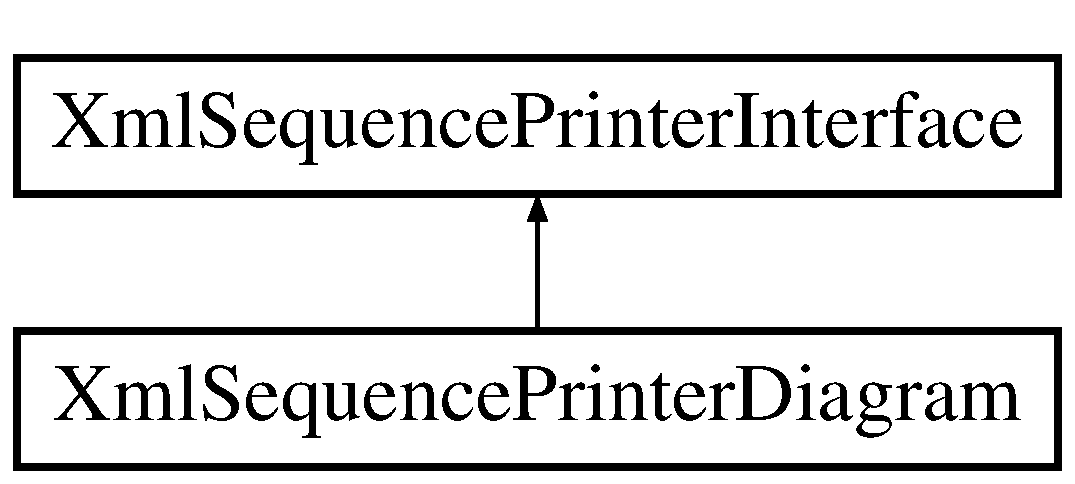
\includegraphics[height=2cm]{class_xml_sequence_printer_diagram}
\end{center}
\end{figure}
\subsection*{Public Member Functions}
\begin{CompactItemize}
\item 
\hyperlink{class_xml_sequence_printer_diagram_a94b897abb072d1d895c2e63dfa066d2}{perform} (\hyperlink{class_xml_sequence}{XmlSequence} \$objXmlSequence)
\item 
\hyperlink{class_xml_sequence_printer_diagram_e80bb8be07efce8abf9af54488d3c616}{setZoom} (\$intZoom)
\item 
\hyperlink{class_xml_sequence_printer_diagram_71fbe6074cf81fab4eee271f16a6f189}{getZoom} ()
\item 
\hyperlink{class_xml_sequence_printer_diagram_bf7cd1d36e6867cefed731112b9ed8e8}{show} ()
\item 
\hyperlink{class_xml_sequence_printer_diagram_eda31caa1d4a613d270b3ca55accd2dd}{showValues} (\hyperlink{class_xml_sequence_message}{XmlSequenceMessage} \$objXmlMessage)
\end{CompactItemize}
\subsection*{Static Public Member Functions}
\begin{CompactItemize}
\item 
static \hyperlink{class_xml_sequence_printer_diagram_c11a145d18a480a3fa4d8404f9aa1649}{getInstance} ()
\end{CompactItemize}
\subsection*{Protected Member Functions}
\begin{CompactItemize}
\item 
\hyperlink{class_xml_sequence_printer_diagram_e7975e1165f4b290bc9ddaba3ae7d5c5}{showHeaders} ()
\item 
\hyperlink{class_xml_sequence_printer_diagram_11f8dd9065dd384aeb6e498578cff669}{showFooter} ()
\end{CompactItemize}
\subsection*{Protected Attributes}
\begin{CompactItemize}
\item 
\hyperlink{class_xml_sequence_printer_diagram_4d24b76a9be3f7a080a5434e5d917912}{\$objXmlSequence}
\item 
\hyperlink{class_xml_sequence_printer_diagram_342c720d4dc17c2b8fd161f3f2579b3a}{\$intMessageWidth} = 300
\item 
\hyperlink{class_xml_sequence_printer_diagram_223b298c0d3af258bfe6a2631ae33ff5}{\$intActorHeaderWidth} = 100
\item 
\hyperlink{class_xml_sequence_printer_diagram_97531ddc90690c05c0feecd57be48006}{\$intActorBarWidth} = 10
\item 
\hyperlink{class_xml_sequence_printer_diagram_dd52069aecd62faf2c555a4dec1ad607}{\$intFont} = 13
\item 
\hyperlink{class_xml_sequence_printer_diagram_6feab15dfe17205a6efca8744c792477}{\$intZoom} = 100
\end{CompactItemize}
\subsection*{Static Protected Attributes}
\begin{CompactItemize}
\item 
static \hyperlink{class_xml_sequence_printer_diagram_bbc670b6771acaff2420cc4feb1624c8}{\$objInstance}
\end{CompactItemize}


\subsection{Member Function Documentation}
\hypertarget{class_xml_sequence_printer_diagram_c11a145d18a480a3fa4d8404f9aa1649}{
\index{XmlSequencePrinterDiagram@{XmlSequencePrinterDiagram}!getInstance@{getInstance}}
\index{getInstance@{getInstance}!XmlSequencePrinterDiagram@{XmlSequencePrinterDiagram}}
\subsubsection[{getInstance}]{\setlength{\rightskip}{0pt plus 5cm}static XmlSequencePrinterDiagram::getInstance ()\hspace{0.3cm}{\tt  \mbox{[}static\mbox{]}}}}
\label{class_xml_sequence_printer_diagram_c11a145d18a480a3fa4d8404f9aa1649}


Return the singleton of the \hyperlink{class_xml_sequence_printer_diagram}{XmlSequencePrinterDiagram}

\begin{Desc}
\item[See also:]\hyperlink{interface_xml_sequence_printer_interface_d488a9fe62e4e3018e482d31497d5e99}{XmlSequencePrinterInterface::getInstance} \end{Desc}
\begin{Desc}
\item[Returns:]\hyperlink{class_xml_sequence_printer_diagram}{XmlSequencePrinterDiagram} \end{Desc}


Implements \hyperlink{interface_xml_sequence_printer_interface_d488a9fe62e4e3018e482d31497d5e99}{XmlSequencePrinterInterface}.\hypertarget{class_xml_sequence_printer_diagram_71fbe6074cf81fab4eee271f16a6f189}{
\index{XmlSequencePrinterDiagram@{XmlSequencePrinterDiagram}!getZoom@{getZoom}}
\index{getZoom@{getZoom}!XmlSequencePrinterDiagram@{XmlSequencePrinterDiagram}}
\subsubsection[{getZoom}]{\setlength{\rightskip}{0pt plus 5cm}XmlSequencePrinterDiagram::getZoom ()}}
\label{class_xml_sequence_printer_diagram_71fbe6074cf81fab4eee271f16a6f189}


Get the zoom of the diagram

\begin{Desc}
\item[Returns:]integer \end{Desc}
\hypertarget{class_xml_sequence_printer_diagram_a94b897abb072d1d895c2e63dfa066d2}{
\index{XmlSequencePrinterDiagram@{XmlSequencePrinterDiagram}!perform@{perform}}
\index{perform@{perform}!XmlSequencePrinterDiagram@{XmlSequencePrinterDiagram}}
\subsubsection[{perform}]{\setlength{\rightskip}{0pt plus 5cm}XmlSequencePrinterDiagram::perform ({\bf XmlSequence} \$ {\em objXmlSequence})}}
\label{class_xml_sequence_printer_diagram_a94b897abb072d1d895c2e63dfa066d2}


Perfom the print process

\begin{Desc}
\item[See also:]XmlSequencePrinterInterface::perform( XmlSequence ) \end{Desc}
\begin{Desc}
\item[Parameters:]
\begin{description}
\item[{\em \hyperlink{class_xml_sequence}{XmlSequence}}]\$objXmlSequence \end{description}
\end{Desc}
\begin{Desc}
\item[Returns:]mixer \end{Desc}


Implements \hyperlink{interface_xml_sequence_printer_interface_68a8066e69c402d49dd0a16a22cfcb6b}{XmlSequencePrinterInterface}.\hypertarget{class_xml_sequence_printer_diagram_e80bb8be07efce8abf9af54488d3c616}{
\index{XmlSequencePrinterDiagram@{XmlSequencePrinterDiagram}!setZoom@{setZoom}}
\index{setZoom@{setZoom}!XmlSequencePrinterDiagram@{XmlSequencePrinterDiagram}}
\subsubsection[{setZoom}]{\setlength{\rightskip}{0pt plus 5cm}XmlSequencePrinterDiagram::setZoom (\$ {\em intZoom})}}
\label{class_xml_sequence_printer_diagram_e80bb8be07efce8abf9af54488d3c616}


Set the zoom of the diagram

\begin{Desc}
\item[Parameters:]
\begin{description}
\item[{\em integer}]\$intZoom \end{description}
\end{Desc}
\begin{Desc}
\item[Returns:]\hyperlink{class_xml_sequence}{XmlSequence} me \end{Desc}
\hypertarget{class_xml_sequence_printer_diagram_bf7cd1d36e6867cefed731112b9ed8e8}{
\index{XmlSequencePrinterDiagram@{XmlSequencePrinterDiagram}!show@{show}}
\index{show@{show}!XmlSequencePrinterDiagram@{XmlSequencePrinterDiagram}}
\subsubsection[{show}]{\setlength{\rightskip}{0pt plus 5cm}XmlSequencePrinterDiagram::show ()}}
\label{class_xml_sequence_printer_diagram_bf7cd1d36e6867cefed731112b9ed8e8}


\hypertarget{class_xml_sequence_printer_diagram_11f8dd9065dd384aeb6e498578cff669}{
\index{XmlSequencePrinterDiagram@{XmlSequencePrinterDiagram}!showFooter@{showFooter}}
\index{showFooter@{showFooter}!XmlSequencePrinterDiagram@{XmlSequencePrinterDiagram}}
\subsubsection[{showFooter}]{\setlength{\rightskip}{0pt plus 5cm}XmlSequencePrinterDiagram::showFooter ()\hspace{0.3cm}{\tt  \mbox{[}protected\mbox{]}}}}
\label{class_xml_sequence_printer_diagram_11f8dd9065dd384aeb6e498578cff669}


Create and return the string of the footer of the html sequence diagram

\begin{Desc}
\item[Returns:]string \end{Desc}
\hypertarget{class_xml_sequence_printer_diagram_e7975e1165f4b290bc9ddaba3ae7d5c5}{
\index{XmlSequencePrinterDiagram@{XmlSequencePrinterDiagram}!showHeaders@{showHeaders}}
\index{showHeaders@{showHeaders}!XmlSequencePrinterDiagram@{XmlSequencePrinterDiagram}}
\subsubsection[{showHeaders}]{\setlength{\rightskip}{0pt plus 5cm}XmlSequencePrinterDiagram::showHeaders ()\hspace{0.3cm}{\tt  \mbox{[}protected\mbox{]}}}}
\label{class_xml_sequence_printer_diagram_e7975e1165f4b290bc9ddaba3ae7d5c5}


Create and return the string of the header of the html sequence diagram

\begin{Desc}
\item[Returns:]string \end{Desc}
\hypertarget{class_xml_sequence_printer_diagram_eda31caa1d4a613d270b3ca55accd2dd}{
\index{XmlSequencePrinterDiagram@{XmlSequencePrinterDiagram}!showValues@{showValues}}
\index{showValues@{showValues}!XmlSequencePrinterDiagram@{XmlSequencePrinterDiagram}}
\subsubsection[{showValues}]{\setlength{\rightskip}{0pt plus 5cm}XmlSequencePrinterDiagram::showValues ({\bf XmlSequenceMessage} \$ {\em objXmlMessage})}}
\label{class_xml_sequence_printer_diagram_eda31caa1d4a613d270b3ca55accd2dd}


Create and return the html of some values of some messages into the html sequence diagram

\begin{Desc}
\item[Parameters:]
\begin{description}
\item[{\em \hyperlink{class_xml_sequence_message}{XmlSequenceMessage}}]\$objXmlMessage \end{description}
\end{Desc}
\begin{Desc}
\item[Returns:]string \end{Desc}


\subsection{Member Data Documentation}
\hypertarget{class_xml_sequence_printer_diagram_97531ddc90690c05c0feecd57be48006}{
\index{XmlSequencePrinterDiagram@{XmlSequencePrinterDiagram}!\$intActorBarWidth@{\$intActorBarWidth}}
\index{\$intActorBarWidth@{\$intActorBarWidth}!XmlSequencePrinterDiagram@{XmlSequencePrinterDiagram}}
\subsubsection[{\$intActorBarWidth}]{\setlength{\rightskip}{0pt plus 5cm}XmlSequencePrinterDiagram::\$intActorBarWidth = 10\hspace{0.3cm}{\tt  \mbox{[}protected\mbox{]}}}}
\label{class_xml_sequence_printer_diagram_97531ddc90690c05c0feecd57be48006}


\hypertarget{class_xml_sequence_printer_diagram_223b298c0d3af258bfe6a2631ae33ff5}{
\index{XmlSequencePrinterDiagram@{XmlSequencePrinterDiagram}!\$intActorHeaderWidth@{\$intActorHeaderWidth}}
\index{\$intActorHeaderWidth@{\$intActorHeaderWidth}!XmlSequencePrinterDiagram@{XmlSequencePrinterDiagram}}
\subsubsection[{\$intActorHeaderWidth}]{\setlength{\rightskip}{0pt plus 5cm}XmlSequencePrinterDiagram::\$intActorHeaderWidth = 100\hspace{0.3cm}{\tt  \mbox{[}protected\mbox{]}}}}
\label{class_xml_sequence_printer_diagram_223b298c0d3af258bfe6a2631ae33ff5}


\hypertarget{class_xml_sequence_printer_diagram_dd52069aecd62faf2c555a4dec1ad607}{
\index{XmlSequencePrinterDiagram@{XmlSequencePrinterDiagram}!\$intFont@{\$intFont}}
\index{\$intFont@{\$intFont}!XmlSequencePrinterDiagram@{XmlSequencePrinterDiagram}}
\subsubsection[{\$intFont}]{\setlength{\rightskip}{0pt plus 5cm}XmlSequencePrinterDiagram::\$intFont = 13\hspace{0.3cm}{\tt  \mbox{[}protected\mbox{]}}}}
\label{class_xml_sequence_printer_diagram_dd52069aecd62faf2c555a4dec1ad607}


\hypertarget{class_xml_sequence_printer_diagram_342c720d4dc17c2b8fd161f3f2579b3a}{
\index{XmlSequencePrinterDiagram@{XmlSequencePrinterDiagram}!\$intMessageWidth@{\$intMessageWidth}}
\index{\$intMessageWidth@{\$intMessageWidth}!XmlSequencePrinterDiagram@{XmlSequencePrinterDiagram}}
\subsubsection[{\$intMessageWidth}]{\setlength{\rightskip}{0pt plus 5cm}XmlSequencePrinterDiagram::\$intMessageWidth = 300\hspace{0.3cm}{\tt  \mbox{[}protected\mbox{]}}}}
\label{class_xml_sequence_printer_diagram_342c720d4dc17c2b8fd161f3f2579b3a}


\hypertarget{class_xml_sequence_printer_diagram_6feab15dfe17205a6efca8744c792477}{
\index{XmlSequencePrinterDiagram@{XmlSequencePrinterDiagram}!\$intZoom@{\$intZoom}}
\index{\$intZoom@{\$intZoom}!XmlSequencePrinterDiagram@{XmlSequencePrinterDiagram}}
\subsubsection[{\$intZoom}]{\setlength{\rightskip}{0pt plus 5cm}XmlSequencePrinterDiagram::\$intZoom = 100\hspace{0.3cm}{\tt  \mbox{[}protected\mbox{]}}}}
\label{class_xml_sequence_printer_diagram_6feab15dfe17205a6efca8744c792477}


\hypertarget{class_xml_sequence_printer_diagram_bbc670b6771acaff2420cc4feb1624c8}{
\index{XmlSequencePrinterDiagram@{XmlSequencePrinterDiagram}!\$objInstance@{\$objInstance}}
\index{\$objInstance@{\$objInstance}!XmlSequencePrinterDiagram@{XmlSequencePrinterDiagram}}
\subsubsection[{\$objInstance}]{\setlength{\rightskip}{0pt plus 5cm}XmlSequencePrinterDiagram::\$objInstance\hspace{0.3cm}{\tt  \mbox{[}static, protected\mbox{]}}}}
\label{class_xml_sequence_printer_diagram_bbc670b6771acaff2420cc4feb1624c8}


\hypertarget{class_xml_sequence_printer_diagram_4d24b76a9be3f7a080a5434e5d917912}{
\index{XmlSequencePrinterDiagram@{XmlSequencePrinterDiagram}!\$objXmlSequence@{\$objXmlSequence}}
\index{\$objXmlSequence@{\$objXmlSequence}!XmlSequencePrinterDiagram@{XmlSequencePrinterDiagram}}
\subsubsection[{\$objXmlSequence}]{\setlength{\rightskip}{0pt plus 5cm}XmlSequencePrinterDiagram::\$objXmlSequence\hspace{0.3cm}{\tt  \mbox{[}protected\mbox{]}}}}
\label{class_xml_sequence_printer_diagram_4d24b76a9be3f7a080a5434e5d917912}




The documentation for this class was generated from the following file:\begin{CompactItemize}
\item 
components/xmlSequence/\hyperlink{_xml_sequence_printer_diagram_8class_8php}{XmlSequencePrinterDiagram.class.php}\end{CompactItemize}

\hypertarget{interface_xml_sequence_printer_interface}{
\section{XmlSequencePrinterInterface Interface Reference}
\label{interface_xml_sequence_printer_interface}\index{XmlSequencePrinterInterface@{XmlSequencePrinterInterface}}
}
Inheritance diagram for XmlSequencePrinterInterface::\begin{figure}[H]
\begin{center}
\leavevmode
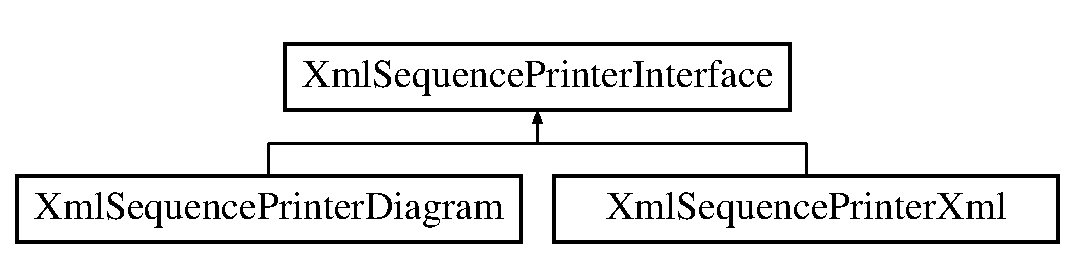
\includegraphics[height=2cm]{interface_xml_sequence_printer_interface}
\end{center}
\end{figure}
\subsection*{Public Member Functions}
\begin{CompactItemize}
\item 
\hyperlink{interface_xml_sequence_printer_interface_68a8066e69c402d49dd0a16a22cfcb6b}{perform} (\hyperlink{class_xml_sequence}{XmlSequence} \$objXmlSequence)
\end{CompactItemize}
\subsection*{Static Public Member Functions}
\begin{CompactItemize}
\item 
static \hyperlink{interface_xml_sequence_printer_interface_d488a9fe62e4e3018e482d31497d5e99}{getInstance} ()
\end{CompactItemize}


\subsection{Member Function Documentation}
\hypertarget{interface_xml_sequence_printer_interface_d488a9fe62e4e3018e482d31497d5e99}{
\index{XmlSequencePrinterInterface@{XmlSequencePrinterInterface}!getInstance@{getInstance}}
\index{getInstance@{getInstance}!XmlSequencePrinterInterface@{XmlSequencePrinterInterface}}
\subsubsection[{getInstance}]{\setlength{\rightskip}{0pt plus 5cm}static XmlSequencePrinterInterface::getInstance ()\hspace{0.3cm}{\tt  \mbox{[}static\mbox{]}}}}
\label{interface_xml_sequence_printer_interface_d488a9fe62e4e3018e482d31497d5e99}


Return the singleton of the \hyperlink{class_xml_sequence_printer_diagram}{XmlSequencePrinterDiagram}

\begin{Desc}
\item[Returns:]\hyperlink{interface_xml_sequence_printer_interface}{XmlSequencePrinterInterface} \end{Desc}


Implemented in \hyperlink{class_xml_sequence_printer_diagram_c11a145d18a480a3fa4d8404f9aa1649}{XmlSequencePrinterDiagram}, and \hyperlink{class_xml_sequence_printer_xml_1c628de89547bd7a6aa509748e562e67}{XmlSequencePrinterXml}.\hypertarget{interface_xml_sequence_printer_interface_68a8066e69c402d49dd0a16a22cfcb6b}{
\index{XmlSequencePrinterInterface@{XmlSequencePrinterInterface}!perform@{perform}}
\index{perform@{perform}!XmlSequencePrinterInterface@{XmlSequencePrinterInterface}}
\subsubsection[{perform}]{\setlength{\rightskip}{0pt plus 5cm}XmlSequencePrinterInterface::perform ({\bf XmlSequence} \$ {\em objXmlSequence})}}
\label{interface_xml_sequence_printer_interface_68a8066e69c402d49dd0a16a22cfcb6b}


Perfom the print process

\begin{Desc}
\item[Parameters:]
\begin{description}
\item[{\em \hyperlink{class_xml_sequence}{XmlSequence}}]\$objXmlSequence \end{description}
\end{Desc}
\begin{Desc}
\item[Returns:]mixer \end{Desc}


Implemented in \hyperlink{class_xml_sequence_printer_diagram_a94b897abb072d1d895c2e63dfa066d2}{XmlSequencePrinterDiagram}, and \hyperlink{class_xml_sequence_printer_xml_7e88c479f35acfc1ce0f053c4dbadb1b}{XmlSequencePrinterXml}.

The documentation for this interface was generated from the following file:\begin{CompactItemize}
\item 
components/xmlSequence/\hyperlink{_xml_sequence_printer_interface_8interface_8php}{XmlSequencePrinterInterface.interface.php}\end{CompactItemize}

\hypertarget{class_xml_sequence_printer_xml}{
\section{XmlSequencePrinterXml Class Reference}
\label{class_xml_sequence_printer_xml}\index{XmlSequencePrinterXml@{XmlSequencePrinterXml}}
}
Inheritance diagram for XmlSequencePrinterXml::\begin{figure}[H]
\begin{center}
\leavevmode
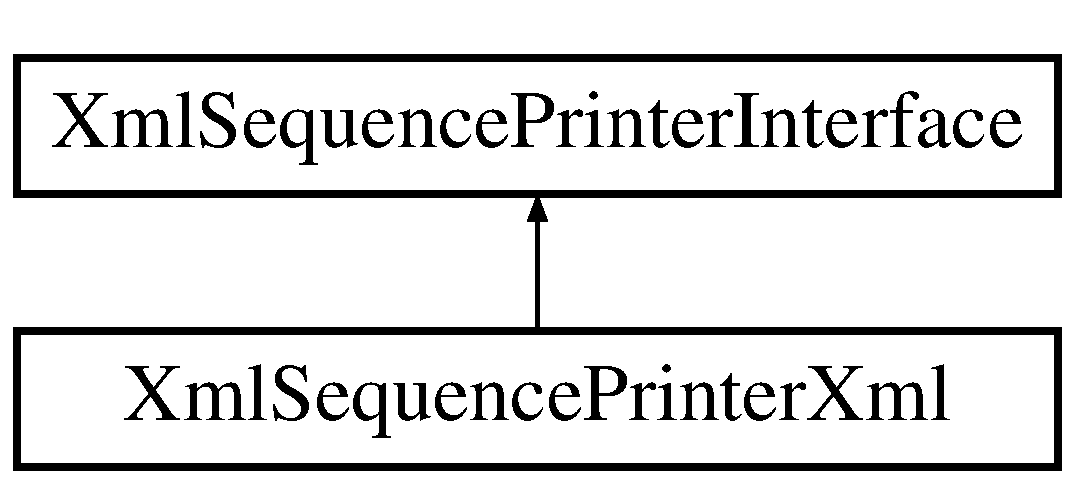
\includegraphics[height=2cm]{class_xml_sequence_printer_xml}
\end{center}
\end{figure}
\subsection*{Public Member Functions}
\begin{CompactItemize}
\item 
\hyperlink{class_xml_sequence_printer_xml_7e88c479f35acfc1ce0f053c4dbadb1b}{perform} (\hyperlink{class_xml_sequence}{XmlSequence} \$objXmlSequence)
\item 
\hyperlink{class_xml_sequence_printer_xml_15a782830da7eeff1fc9746d223452ac}{createXml} ()
\item 
\hyperlink{class_xml_sequence_printer_xml_534160e28dc8623f138311e4a73be081}{createXmlHeader} ()
\item 
\hyperlink{class_xml_sequence_printer_xml_774ffc0433f81a35080033382a39d525}{createXmlFooter} ()
\end{CompactItemize}
\subsection*{Static Public Member Functions}
\begin{CompactItemize}
\item 
static \hyperlink{class_xml_sequence_printer_xml_1c628de89547bd7a6aa509748e562e67}{getInstance} ()
\end{CompactItemize}
\subsection*{Protected Attributes}
\begin{CompactItemize}
\item 
\hyperlink{class_xml_sequence_printer_xml_c24cec88eff41ddb99b215601cd6f5d8}{\$objXmlSequence}
\end{CompactItemize}
\subsection*{Static Protected Attributes}
\begin{CompactItemize}
\item 
static \hyperlink{class_xml_sequence_printer_xml_e633ac1e15f76e165c7a6d599de36231}{\$objInstance}
\end{CompactItemize}


\subsection{Member Function Documentation}
\hypertarget{class_xml_sequence_printer_xml_15a782830da7eeff1fc9746d223452ac}{
\index{XmlSequencePrinterXml@{XmlSequencePrinterXml}!createXml@{createXml}}
\index{createXml@{createXml}!XmlSequencePrinterXml@{XmlSequencePrinterXml}}
\subsubsection[{createXml}]{\setlength{\rightskip}{0pt plus 5cm}XmlSequencePrinterXml::createXml ()}}
\label{class_xml_sequence_printer_xml_15a782830da7eeff1fc9746d223452ac}


Create and return the xml of the sequence diagram object

\begin{Desc}
\item[See also:]\hyperlink{class_xml_sequence_printer_xml_534160e28dc8623f138311e4a73be081}{XmlSequencePrinterXml::createXmlHeader()} 

XmlSequencePrinterXml::createXmlActors() 

\hyperlink{class_xml_sequence_printer_xml_774ffc0433f81a35080033382a39d525}{XmlSequencePrinterXml::createXmlFooter()} \end{Desc}
\begin{Desc}
\item[Returns:]string \end{Desc}
\hypertarget{class_xml_sequence_printer_xml_774ffc0433f81a35080033382a39d525}{
\index{XmlSequencePrinterXml@{XmlSequencePrinterXml}!createXmlFooter@{createXmlFooter}}
\index{createXmlFooter@{createXmlFooter}!XmlSequencePrinterXml@{XmlSequencePrinterXml}}
\subsubsection[{createXmlFooter}]{\setlength{\rightskip}{0pt plus 5cm}XmlSequencePrinterXml::createXmlFooter ()}}
\label{class_xml_sequence_printer_xml_774ffc0433f81a35080033382a39d525}


Create and return the footer slice of the xml

\begin{Desc}
\item[Returns:]string \end{Desc}
\hypertarget{class_xml_sequence_printer_xml_534160e28dc8623f138311e4a73be081}{
\index{XmlSequencePrinterXml@{XmlSequencePrinterXml}!createXmlHeader@{createXmlHeader}}
\index{createXmlHeader@{createXmlHeader}!XmlSequencePrinterXml@{XmlSequencePrinterXml}}
\subsubsection[{createXmlHeader}]{\setlength{\rightskip}{0pt plus 5cm}XmlSequencePrinterXml::createXmlHeader ()}}
\label{class_xml_sequence_printer_xml_534160e28dc8623f138311e4a73be081}


Create and return the header slice of the xml

\begin{Desc}
\item[Returns:]string \end{Desc}
\hypertarget{class_xml_sequence_printer_xml_1c628de89547bd7a6aa509748e562e67}{
\index{XmlSequencePrinterXml@{XmlSequencePrinterXml}!getInstance@{getInstance}}
\index{getInstance@{getInstance}!XmlSequencePrinterXml@{XmlSequencePrinterXml}}
\subsubsection[{getInstance}]{\setlength{\rightskip}{0pt plus 5cm}static XmlSequencePrinterXml::getInstance ()\hspace{0.3cm}{\tt  \mbox{[}static\mbox{]}}}}
\label{class_xml_sequence_printer_xml_1c628de89547bd7a6aa509748e562e67}


Return the singleton of the \hyperlink{class_xml_sequence_printer_xml}{XmlSequencePrinterXml}

\begin{Desc}
\item[See also:]\hyperlink{interface_xml_sequence_printer_interface_d488a9fe62e4e3018e482d31497d5e99}{XmlSequencePrinterInterface::getInstance} \end{Desc}
\begin{Desc}
\item[Returns:]\hyperlink{class_xml_sequence_printer_xml}{XmlSequencePrinterXml} \end{Desc}


Implements \hyperlink{interface_xml_sequence_printer_interface_d488a9fe62e4e3018e482d31497d5e99}{XmlSequencePrinterInterface}.\hypertarget{class_xml_sequence_printer_xml_7e88c479f35acfc1ce0f053c4dbadb1b}{
\index{XmlSequencePrinterXml@{XmlSequencePrinterXml}!perform@{perform}}
\index{perform@{perform}!XmlSequencePrinterXml@{XmlSequencePrinterXml}}
\subsubsection[{perform}]{\setlength{\rightskip}{0pt plus 5cm}XmlSequencePrinterXml::perform ({\bf XmlSequence} \$ {\em objXmlSequence})}}
\label{class_xml_sequence_printer_xml_7e88c479f35acfc1ce0f053c4dbadb1b}


Perfom the print process

\begin{Desc}
\item[See also:]XmlSequencePrinterInterface::perform( XmlSequence ) \end{Desc}
\begin{Desc}
\item[Parameters:]
\begin{description}
\item[{\em \hyperlink{class_xml_sequence}{XmlSequence}}]\$objXmlSequence \end{description}
\end{Desc}
\begin{Desc}
\item[Returns:]mixer \end{Desc}


Implements \hyperlink{interface_xml_sequence_printer_interface_68a8066e69c402d49dd0a16a22cfcb6b}{XmlSequencePrinterInterface}.

\subsection{Member Data Documentation}
\hypertarget{class_xml_sequence_printer_xml_e633ac1e15f76e165c7a6d599de36231}{
\index{XmlSequencePrinterXml@{XmlSequencePrinterXml}!\$objInstance@{\$objInstance}}
\index{\$objInstance@{\$objInstance}!XmlSequencePrinterXml@{XmlSequencePrinterXml}}
\subsubsection[{\$objInstance}]{\setlength{\rightskip}{0pt plus 5cm}XmlSequencePrinterXml::\$objInstance\hspace{0.3cm}{\tt  \mbox{[}static, protected\mbox{]}}}}
\label{class_xml_sequence_printer_xml_e633ac1e15f76e165c7a6d599de36231}


\hypertarget{class_xml_sequence_printer_xml_c24cec88eff41ddb99b215601cd6f5d8}{
\index{XmlSequencePrinterXml@{XmlSequencePrinterXml}!\$objXmlSequence@{\$objXmlSequence}}
\index{\$objXmlSequence@{\$objXmlSequence}!XmlSequencePrinterXml@{XmlSequencePrinterXml}}
\subsubsection[{\$objXmlSequence}]{\setlength{\rightskip}{0pt plus 5cm}XmlSequencePrinterXml::\$objXmlSequence\hspace{0.3cm}{\tt  \mbox{[}protected\mbox{]}}}}
\label{class_xml_sequence_printer_xml_c24cec88eff41ddb99b215601cd6f5d8}




The documentation for this class was generated from the following file:\begin{CompactItemize}
\item 
components/xmlSequence/\hyperlink{_xml_sequence_printer_xml_8class_8php}{XmlSequencePrinterXml.class.php}\end{CompactItemize}

\hypertarget{class_xml_sequence_value}{
\section{XmlSequenceValue Class Reference}
\label{class_xml_sequence_value}\index{XmlSequenceValue@{XmlSequenceValue}}
}
\subsection*{Public Member Functions}
\begin{CompactItemize}
\item 
\hyperlink{class_xml_sequence_value_c05d9184d52b7a34210a801767bef213}{setName} (\$strName)
\item 
\hyperlink{class_xml_sequence_value_3d0963e68bb313b163a73f2803c64600}{getName} ()
\item 
\hyperlink{class_xml_sequence_value_b5d79fa8a006bc1c112844b24f3e4897}{setValue} (\$strValue)
\item 
\hyperlink{class_xml_sequence_value_c0bc18784b182c89fcfd276625aef435}{getValue} ()
\end{CompactItemize}
\subsection*{Protected Attributes}
\begin{CompactItemize}
\item 
\hyperlink{class_xml_sequence_value_90edf7538a74be8ac5ce46baaf203382}{\$strName}
\item 
\hyperlink{class_xml_sequence_value_4ca01dcd54c8197f45702984773b68a4}{\$strValue}
\end{CompactItemize}


\subsection{Detailed Description}
Object with the values send into the message \begin{Desc}
\item[Author:]Thiago Henrique Ramos da Mata $<$\href{mailto:thiago.henrique.mata@gmail.com}{\tt thiago.henrique.mata@gmail.com}$>$ \end{Desc}


\subsection{Member Function Documentation}
\hypertarget{class_xml_sequence_value_3d0963e68bb313b163a73f2803c64600}{
\index{XmlSequenceValue@{XmlSequenceValue}!getName@{getName}}
\index{getName@{getName}!XmlSequenceValue@{XmlSequenceValue}}
\subsubsection[{getName}]{\setlength{\rightskip}{0pt plus 5cm}getName ()}}
\label{class_xml_sequence_value_3d0963e68bb313b163a73f2803c64600}


set the name of the attribute value

\begin{Desc}
\item[See also:]XmlSequenceValue::setName( string ) 

XmlSequenceValue-$>$strName \end{Desc}
\begin{Desc}
\item[Returns:]string \end{Desc}


\begin{Code}\begin{verbatim}49     {
50         return $this->strName;
51     }
\end{verbatim}
\end{Code}


\hypertarget{class_xml_sequence_value_c0bc18784b182c89fcfd276625aef435}{
\index{XmlSequenceValue@{XmlSequenceValue}!getValue@{getValue}}
\index{getValue@{getValue}!XmlSequenceValue@{XmlSequenceValue}}
\subsubsection[{getValue}]{\setlength{\rightskip}{0pt plus 5cm}getValue ()}}
\label{class_xml_sequence_value_c0bc18784b182c89fcfd276625aef435}


set the value of the attribute

\begin{Desc}
\item[See also:]XmlSequenceValue::setValue( string ) 

XmlSequenceValue-$>$strValue \end{Desc}
\begin{Desc}
\item[Returns:]string \end{Desc}


\begin{Code}\begin{verbatim}75     {
76         return $this->strValue;
77     }
\end{verbatim}
\end{Code}


\hypertarget{class_xml_sequence_value_c05d9184d52b7a34210a801767bef213}{
\index{XmlSequenceValue@{XmlSequenceValue}!setName@{setName}}
\index{setName@{setName}!XmlSequenceValue@{XmlSequenceValue}}
\subsubsection[{setName}]{\setlength{\rightskip}{0pt plus 5cm}setName (\$ {\em strName})}}
\label{class_xml_sequence_value_c05d9184d52b7a34210a801767bef213}


Set the name of the attribute value

\begin{Desc}
\item[See also:]\hyperlink{class_xml_sequence_value_3d0963e68bb313b163a73f2803c64600}{XmlSequenceValue::getName()} 

XmlSequenceValue-$>$strName \end{Desc}
\begin{Desc}
\item[Parameters:]
\begin{description}
\item[{\em string}]\$strName \end{description}
\end{Desc}
\begin{Desc}
\item[Returns:]\hyperlink{class_xml_sequence_value}{XmlSequenceValue} me \end{Desc}


\begin{Code}\begin{verbatim}36     {
37         $this->strName = $strName;
38         return $this;
39     }
\end{verbatim}
\end{Code}


\hypertarget{class_xml_sequence_value_b5d79fa8a006bc1c112844b24f3e4897}{
\index{XmlSequenceValue@{XmlSequenceValue}!setValue@{setValue}}
\index{setValue@{setValue}!XmlSequenceValue@{XmlSequenceValue}}
\subsubsection[{setValue}]{\setlength{\rightskip}{0pt plus 5cm}setValue (\$ {\em strValue})}}
\label{class_xml_sequence_value_b5d79fa8a006bc1c112844b24f3e4897}


Set the value of the attribute

\begin{Desc}
\item[See also:]\hyperlink{class_xml_sequence_value_c0bc18784b182c89fcfd276625aef435}{XmlSequenceValue::getValue()} 

XmlSequenceValue-$>$strValue \end{Desc}
\begin{Desc}
\item[Parameters:]
\begin{description}
\item[{\em string}]\$strValue \end{description}
\end{Desc}
\begin{Desc}
\item[Returns:]\hyperlink{class_xml_sequence_value}{XmlSequenceValue} me \end{Desc}


\begin{Code}\begin{verbatim}62     {
63         $this->strValue = $strValue;
64         return $this;
65     }
\end{verbatim}
\end{Code}




\subsection{Member Data Documentation}
\hypertarget{class_xml_sequence_value_90edf7538a74be8ac5ce46baaf203382}{
\index{XmlSequenceValue@{XmlSequenceValue}!\$strName@{\$strName}}
\index{\$strName@{\$strName}!XmlSequenceValue@{XmlSequenceValue}}
\subsubsection[{\$strName}]{\setlength{\rightskip}{0pt plus 5cm}\$strName\hspace{0.3cm}{\tt  \mbox{[}protected\mbox{]}}}}
\label{class_xml_sequence_value_90edf7538a74be8ac5ce46baaf203382}


Name of the attribute

string \hypertarget{class_xml_sequence_value_4ca01dcd54c8197f45702984773b68a4}{
\index{XmlSequenceValue@{XmlSequenceValue}!\$strValue@{\$strValue}}
\index{\$strValue@{\$strValue}!XmlSequenceValue@{XmlSequenceValue}}
\subsubsection[{\$strValue}]{\setlength{\rightskip}{0pt plus 5cm}\$strValue\hspace{0.3cm}{\tt  \mbox{[}protected\mbox{]}}}}
\label{class_xml_sequence_value_4ca01dcd54c8197f45702984773b68a4}


Value of the attribute

string 

The documentation for this class was generated from the following file:\begin{CompactItemize}
\item 
components/xmlSequence/\hyperlink{_xml_sequence_value_8class_8php}{XmlSequenceValue.class.php}\end{CompactItemize}

\chapter{File Documentation}
\hypertarget{__start_8php}{
\section{\_\-start.php File Reference}
\label{__start_8php}\index{\_\-start.php@{\_\-start.php}}
}
\subsection*{Enumerations}
\begin{CompactItemize}
\item 
enum \hyperlink{__start_8php_bceef7ce0317a0230c7163f52877e667}{PATH\_\-CODE\_\-TO\_\-DIAGRAM} 
\item 
enum \hyperlink{__start_8php_0227eeec0798e41bef3990e74ab2cde2}{PATH\_\-CODE\_\-TO\_\-DIAGRAM\_\-COMPONENT} 
\end{CompactItemize}


\subsection{Enumeration Type Documentation}
\hypertarget{__start_8php_bceef7ce0317a0230c7163f52877e667}{
\index{\_\-start.php@{\_\-start.php}!PATH\_\-CODE\_\-TO\_\-DIAGRAM@{PATH\_\-CODE\_\-TO\_\-DIAGRAM}}
\index{PATH\_\-CODE\_\-TO\_\-DIAGRAM@{PATH\_\-CODE\_\-TO\_\-DIAGRAM}!_start.php@{\_\-start.php}}
\subsubsection[{PATH\_\-CODE\_\-TO\_\-DIAGRAM}]{\setlength{\rightskip}{0pt plus 5cm}enum {\bf PATH\_\-CODE\_\-TO\_\-DIAGRAM}}}
\label{__start_8php_bceef7ce0317a0230c7163f52877e667}


\hypertarget{__start_8php_0227eeec0798e41bef3990e74ab2cde2}{
\index{\_\-start.php@{\_\-start.php}!PATH\_\-CODE\_\-TO\_\-DIAGRAM\_\-COMPONENT@{PATH\_\-CODE\_\-TO\_\-DIAGRAM\_\-COMPONENT}}
\index{PATH\_\-CODE\_\-TO\_\-DIAGRAM\_\-COMPONENT@{PATH\_\-CODE\_\-TO\_\-DIAGRAM\_\-COMPONENT}!_start.php@{\_\-start.php}}
\subsubsection[{PATH\_\-CODE\_\-TO\_\-DIAGRAM\_\-COMPONENT}]{\setlength{\rightskip}{0pt plus 5cm}enum {\bf PATH\_\-CODE\_\-TO\_\-DIAGRAM\_\-COMPONENT}}}
\label{__start_8php_0227eeec0798e41bef3990e74ab2cde2}



\hypertarget{components_2__start_8php}{
\section{components/\_\-start.php File Reference}
\label{components_2__start_8php}\index{components/\_\-start.php@{components/\_\-start.php}}
}
\subsection*{Enumerations}
\begin{CompactItemize}
\item 
enum \hyperlink{components_2__start_8php_a354c4c2689d1d4fa7fd1f4e940a6b2a}{COMPONENTS\_\-PATH} 
\end{CompactItemize}


\subsection{Enumeration Type Documentation}
\hypertarget{components_2__start_8php_a354c4c2689d1d4fa7fd1f4e940a6b2a}{
\index{components/\_\-start.php@{components/\_\-start.php}!COMPONENTS\_\-PATH@{COMPONENTS\_\-PATH}}
\index{COMPONENTS\_\-PATH@{COMPONENTS\_\-PATH}!components/_start.php@{components/\_\-start.php}}
\subsubsection[{COMPONENTS\_\-PATH}]{\setlength{\rightskip}{0pt plus 5cm}enum {\bf COMPONENTS\_\-PATH}}}
\label{components_2__start_8php_a354c4c2689d1d4fa7fd1f4e940a6b2a}



\hypertarget{components_2backtrace_2__start_8php}{
\section{components/backtrace/\_\-start.php File Reference}
\label{components_2backtrace_2__start_8php}\index{components/backtrace/\_\-start.php@{components/backtrace/\_\-start.php}}
}
\subsection*{Namespaces}
\begin{CompactItemize}
\item 
namespace \hyperlink{namespacebacktrace}{backtrace}
\end{CompactItemize}

\hypertarget{components_2code_instrumentation_2__start_8php}{
\section{components/codeInstrumentation/\_\-start.php File Reference}
\label{components_2code_instrumentation_2__start_8php}\index{components/codeInstrumentation/\_\-start.php@{components/codeInstrumentation/\_\-start.php}}
}
\subsection*{Namespaces}
\begin{CompactItemize}
\item 
namespace \hyperlink{namespace_code_instrumentation}{CodeInstrumentation}
\end{CompactItemize}

\hypertarget{components_2code_instrumentation_2example_2__start_8php}{
\section{components/codeInstrumentation/example/\_\-start.php File Reference}
\label{components_2code_instrumentation_2example_2__start_8php}\index{components/codeInstrumentation/example/\_\-start.php@{components/codeInstrumentation/example/\_\-start.php}}
}

\hypertarget{components_2code_reflection_2__start_8php}{
\section{components/codeReflection/\_\-start.php File Reference}
\label{components_2code_reflection_2__start_8php}\index{components/codeReflection/\_\-start.php@{components/codeReflection/\_\-start.php}}
}
\subsection*{Namespaces}
\begin{CompactItemize}
\item 
namespace \hyperlink{namespace_code_reflection}{CodeReflection}
\end{CompactItemize}

\hypertarget{components_2code_reflection_2example_2__start_8php}{
\section{components/codeReflection/example/\_\-start.php File Reference}
\label{components_2code_reflection_2example_2__start_8php}\index{components/codeReflection/example/\_\-start.php@{components/codeReflection/example/\_\-start.php}}
}

\hypertarget{components_2code_to_diagram_2__start_8php}{
\section{components/codeToDiagram/\_\-start.php File Reference}
\label{components_2code_to_diagram_2__start_8php}\index{components/codeToDiagram/\_\-start.php@{components/codeToDiagram/\_\-start.php}}
}
\subsection*{Namespaces}
\begin{CompactItemize}
\item 
namespace \hyperlink{namespace_code_to_diagram}{CodeToDiagram}
\end{CompactItemize}

\hypertarget{components_2extended_reflection_2__start_8php}{
\section{components/extendedReflection/\_\-start.php File Reference}
\label{components_2extended_reflection_2__start_8php}\index{components/extendedReflection/\_\-start.php@{components/extendedReflection/\_\-start.php}}
}
\subsection*{Namespaces}
\begin{CompactItemize}
\item 
namespace \hyperlink{namespace_extended_reflection}{ExtendedReflection}
\end{CompactItemize}

\hypertarget{components_2library_2__start_8php}{
\section{components/library/\_\-start.php File Reference}
\label{components_2library_2__start_8php}\index{components/library/\_\-start.php@{components/library/\_\-start.php}}
}

\hypertarget{components_2library_2example_2__start_8php}{
\section{components/library/example/\_\-start.php File Reference}
\label{components_2library_2example_2__start_8php}\index{components/library/example/\_\-start.php@{components/library/example/\_\-start.php}}
}

\hypertarget{components_2xml_sequence_2__start_8php}{
\section{components/xmlSequence/\_\-start.php File Reference}
\label{components_2xml_sequence_2__start_8php}\index{components/xmlSequence/\_\-start.php@{components/xmlSequence/\_\-start.php}}
}
\subsection*{Namespaces}
\begin{CompactItemize}
\item 
namespace \hyperlink{namespace_xml_sequence}{XmlSequence}
\end{CompactItemize}

\hypertarget{_back_trace_8php}{
\section{components/backtrace/BackTrace.php File Reference}
\label{_back_trace_8php}\index{components/backtrace/BackTrace.php@{components/backtrace/BackTrace.php}}
}
\subsection*{Classes}
\begin{CompactItemize}
\item 
class \hyperlink{class_back_trace}{BackTrace}
\end{CompactItemize}
\subsection*{Namespaces}
\begin{CompactItemize}
\item 
namespace \hyperlink{namespacebacktrace}{backtrace}
\end{CompactItemize}

\hypertarget{_back_trace_explain_8php}{
\section{components/backtrace/BackTraceExplain.php File Reference}
\label{_back_trace_explain_8php}\index{components/backtrace/BackTraceExplain.php@{components/backtrace/BackTraceExplain.php}}
}
\subsection*{Classes}
\begin{CompactItemize}
\item 
class \hyperlink{class_back_trace_explain}{BackTraceExplain}
\end{CompactItemize}
\subsection*{Namespaces}
\begin{CompactItemize}
\item 
namespace \hyperlink{namespacebacktrace}{backtrace}
\end{CompactItemize}

\hypertarget{_code_instrumentation_class_8class_8php}{
\section{components/codeInstrumentation/CodeInstrumentationClass.class.php File Reference}
\label{_code_instrumentation_class_8class_8php}\index{components/codeInstrumentation/CodeInstrumentationClass.class.php@{components/codeInstrumentation/CodeInstrumentationClass.class.php}}
}
\subsection*{Namespaces}
\begin{CompactItemize}
\item 
namespace \hyperlink{namespace_code_instrumentation}{CodeInstrumentation}
\end{CompactItemize}

\hypertarget{_code_instrumentation_exception_8class_8php}{
\section{components/codeInstrumentation/CodeInstrumentationException.class.php File Reference}
\label{_code_instrumentation_exception_8class_8php}\index{components/codeInstrumentation/CodeInstrumentationException.class.php@{components/codeInstrumentation/CodeInstrumentationException.class.php}}
}
\subsection*{Classes}
\begin{CompactItemize}
\item 
class \hyperlink{class_code_instrumentation_exception}{CodeInstrumentationException}
\end{CompactItemize}
\subsection*{Namespaces}
\begin{CompactItemize}
\item 
namespace \hyperlink{namespace_code_instrumentation}{CodeInstrumentation}
\end{CompactItemize}

\hypertarget{_code_instrumentation_function_8class_8php}{
\section{components/codeInstrumentation/CodeInstrumentationFunction.class.php File Reference}
\label{_code_instrumentation_function_8class_8php}\index{components/codeInstrumentation/CodeInstrumentationFunction.class.php@{components/codeInstrumentation/CodeInstrumentationFunction.class.php}}
}
\subsection*{Classes}
\begin{CompactItemize}
\item 
class \hyperlink{class_code_instrumentation_function}{CodeInstrumentationFunction}
\end{CompactItemize}
\subsection*{Namespaces}
\begin{CompactItemize}
\item 
namespace \hyperlink{namespace_code_instrumentation}{CodeInstrumentation}
\end{CompactItemize}

\hypertarget{_code_instrumentation_method_8class_8php}{
\section{components/codeInstrumentation/CodeInstrumentationMethod.class.php File Reference}
\label{_code_instrumentation_method_8class_8php}\index{components/codeInstrumentation/CodeInstrumentationMethod.class.php@{components/codeInstrumentation/CodeInstrumentationMethod.class.php}}
}
\subsection*{Classes}
\begin{CompactItemize}
\item 
class \hyperlink{class_code_instrumentation_method}{CodeInstrumentationMethod}
\end{CompactItemize}
\subsection*{Namespaces}
\begin{CompactItemize}
\item 
namespace \hyperlink{namespace_code_instrumentation}{CodeInstrumentation}
\end{CompactItemize}

\hypertarget{_code_instrumentation_parameter_8class_8php}{
\section{components/codeInstrumentation/CodeInstrumentationParameter.class.php File Reference}
\label{_code_instrumentation_parameter_8class_8php}\index{components/codeInstrumentation/CodeInstrumentationParameter.class.php@{components/codeInstrumentation/CodeInstrumentationParameter.class.php}}
}
\subsection*{Classes}
\begin{CompactItemize}
\item 
class \hyperlink{class_code_instrumentation_parameter}{CodeInstrumentationParameter}
\end{CompactItemize}
\subsection*{Namespaces}
\begin{CompactItemize}
\item 
namespace \hyperlink{namespace_code_instrumentation}{CodeInstrumentation}
\end{CompactItemize}

\hypertarget{_code_instrumentation_property_8class_8php}{
\section{components/codeInstrumentation/CodeInstrumentationProperty.class.php File Reference}
\label{_code_instrumentation_property_8class_8php}\index{components/codeInstrumentation/CodeInstrumentationProperty.class.php@{components/codeInstrumentation/CodeInstrumentationProperty.class.php}}
}
\subsection*{Classes}
\begin{CompactItemize}
\item 
class \hyperlink{class_code_instrumentation_property}{CodeInstrumentationProperty}
\end{CompactItemize}
\subsection*{Namespaces}
\begin{CompactItemize}
\item 
namespace \hyperlink{namespace_code_instrumentation}{CodeInstrumentation}
\end{CompactItemize}

\hypertarget{_code_instrumentation_receiver_8class_8php}{
\section{components/codeInstrumentation/CodeInstrumentationReceiver.class.php File Reference}
\label{_code_instrumentation_receiver_8class_8php}\index{components/codeInstrumentation/CodeInstrumentationReceiver.class.php@{components/codeInstrumentation/CodeInstrumentationReceiver.class.php}}
}
\subsection*{Classes}
\begin{CompactItemize}
\item 
class \hyperlink{class_code_instrumentation_receiver}{CodeInstrumentationReceiver}
\end{CompactItemize}
\subsection*{Namespaces}
\begin{CompactItemize}
\item 
namespace \hyperlink{namespace_code_instrumentation}{CodeInstrumentation}
\end{CompactItemize}

\hypertarget{code_instrumentation_2example_2test1_8php}{
\section{components/codeInstrumentation/example/test1.php File Reference}
\label{code_instrumentation_2example_2test1_8php}\index{components/codeInstrumentation/example/test1.php@{components/codeInstrumentation/example/test1.php}}
}
\subsection*{Enumerations}
\begin{CompactItemize}
\item 
enum \hyperlink{code_instrumentation_2example_2test1_8php_b72f88470e4eee5518bfc7c908101d80}{PUBLIC\_\-PATH} 
\item 
enum \hyperlink{code_instrumentation_2example_2test1_8php_58763391df8832eea0c173fe59e5c977}{CALLER\_\-PATH} 
\end{CompactItemize}
\subsection*{Variables}
\begin{CompactItemize}
\item 
\hyperlink{code_instrumentation_2example_2test1_8php_78bb668948bf961e4e27227e71de5850}{\$strBigFile}
\item 
\hyperlink{code_instrumentation_2example_2test1_8php_dff853bfc3335950f89bfb9e1a779c7e}{\$oReflectionCode} = new CodeInstrumentationClass( \char`\"{}temp\_\-fatorial\char`\"{} , \$strBigFile )
\item 
\hyperlink{code_instrumentation_2example_2test1_8php_882f0b62de6f379d0e0cf88ef6658601}{\$strNewCode} = \$oReflectionCode $\rightarrow$ getCode()
\item 
\hyperlink{code_instrumentation_2example_2test1_8php_e72f9ac2779bbc5e49a4a9df50c17c73}{\$objTest} = new fatorial( 2 )
\item 
\hyperlink{code_instrumentation_2example_2test1_8php_da23b058075209c6506f7b0b1bb0d5bf}{\$objSimpleXml} = simplexml\_\-load\_\-string( CodeInstrumentationReceiver::getInstance() $\rightarrow$ getXmlSequence() $\rightarrow$ createXml() )
\end{CompactItemize}


\subsection{Enumeration Type Documentation}
\hypertarget{code_instrumentation_2example_2test1_8php_58763391df8832eea0c173fe59e5c977}{
\index{codeInstrumentation/example/test1.php@{codeInstrumentation/example/test1.php}!CALLER\_\-PATH@{CALLER\_\-PATH}}
\index{CALLER\_\-PATH@{CALLER\_\-PATH}!codeInstrumentation/example/test1.php@{codeInstrumentation/example/test1.php}}
\subsubsection[{CALLER\_\-PATH}]{\setlength{\rightskip}{0pt plus 5cm}enum {\bf CALLER\_\-PATH}}}
\label{code_instrumentation_2example_2test1_8php_58763391df8832eea0c173fe59e5c977}


\hypertarget{code_instrumentation_2example_2test1_8php_b72f88470e4eee5518bfc7c908101d80}{
\index{codeInstrumentation/example/test1.php@{codeInstrumentation/example/test1.php}!PUBLIC\_\-PATH@{PUBLIC\_\-PATH}}
\index{PUBLIC\_\-PATH@{PUBLIC\_\-PATH}!codeInstrumentation/example/test1.php@{codeInstrumentation/example/test1.php}}
\subsubsection[{PUBLIC\_\-PATH}]{\setlength{\rightskip}{0pt plus 5cm}enum {\bf PUBLIC\_\-PATH}}}
\label{code_instrumentation_2example_2test1_8php_b72f88470e4eee5518bfc7c908101d80}




\subsection{Variable Documentation}
\hypertarget{code_instrumentation_2example_2test1_8php_da23b058075209c6506f7b0b1bb0d5bf}{
\index{codeInstrumentation/example/test1.php@{codeInstrumentation/example/test1.php}!\$objSimpleXml@{\$objSimpleXml}}
\index{\$objSimpleXml@{\$objSimpleXml}!codeInstrumentation/example/test1.php@{codeInstrumentation/example/test1.php}}
\subsubsection[{\$objSimpleXml}]{\setlength{\rightskip}{0pt plus 5cm}\$objSimpleXml = simplexml\_\-load\_\-string( CodeInstrumentationReceiver::getInstance() $\rightarrow$ getXmlSequence() $\rightarrow$ createXml() )}}
\label{code_instrumentation_2example_2test1_8php_da23b058075209c6506f7b0b1bb0d5bf}


\hypertarget{code_instrumentation_2example_2test1_8php_e72f9ac2779bbc5e49a4a9df50c17c73}{
\index{codeInstrumentation/example/test1.php@{codeInstrumentation/example/test1.php}!\$objTest@{\$objTest}}
\index{\$objTest@{\$objTest}!codeInstrumentation/example/test1.php@{codeInstrumentation/example/test1.php}}
\subsubsection[{\$objTest}]{\setlength{\rightskip}{0pt plus 5cm}\$objTest = new fatorial( 2 )}}
\label{code_instrumentation_2example_2test1_8php_e72f9ac2779bbc5e49a4a9df50c17c73}


\hypertarget{code_instrumentation_2example_2test1_8php_dff853bfc3335950f89bfb9e1a779c7e}{
\index{codeInstrumentation/example/test1.php@{codeInstrumentation/example/test1.php}!\$oReflectionCode@{\$oReflectionCode}}
\index{\$oReflectionCode@{\$oReflectionCode}!codeInstrumentation/example/test1.php@{codeInstrumentation/example/test1.php}}
\subsubsection[{\$oReflectionCode}]{\setlength{\rightskip}{0pt plus 5cm}\$oReflectionCode = new CodeInstrumentationClass( \char`\"{}temp\_\-fatorial\char`\"{} , \$strBigFile )}}
\label{code_instrumentation_2example_2test1_8php_dff853bfc3335950f89bfb9e1a779c7e}


\hypertarget{code_instrumentation_2example_2test1_8php_78bb668948bf961e4e27227e71de5850}{
\index{codeInstrumentation/example/test1.php@{codeInstrumentation/example/test1.php}!\$strBigFile@{\$strBigFile}}
\index{\$strBigFile@{\$strBigFile}!codeInstrumentation/example/test1.php@{codeInstrumentation/example/test1.php}}
\subsubsection[{\$strBigFile}]{\setlength{\rightskip}{0pt plus 5cm}\$strBigFile}}
\label{code_instrumentation_2example_2test1_8php_78bb668948bf961e4e27227e71de5850}


\textbf{Initial value:}

\begin{Code}\begin{verbatim} '
class fatorial
{
    protected $n;

    public function __construct( $n )
    {
        $this->n = $n;
    }

    public function calc()
    {
        if ($this->n < 2)
        {
            return 1;
        }
        else
        {
            $objFat = new Fatorial( $this->n - 1 );
            return $this->n * $objFat->calc();
        }
    }
};
'
\end{verbatim}
\end{Code}
\hypertarget{code_instrumentation_2example_2test1_8php_882f0b62de6f379d0e0cf88ef6658601}{
\index{codeInstrumentation/example/test1.php@{codeInstrumentation/example/test1.php}!\$strNewCode@{\$strNewCode}}
\index{\$strNewCode@{\$strNewCode}!codeInstrumentation/example/test1.php@{codeInstrumentation/example/test1.php}}
\subsubsection[{\$strNewCode}]{\setlength{\rightskip}{0pt plus 5cm}\$strNewCode = \$oReflectionCode $\rightarrow$ getCode()}}
\label{code_instrumentation_2example_2test1_8php_882f0b62de6f379d0e0cf88ef6658601}



\hypertarget{code_reflection_2example_2test1_8php}{
\section{components/codeReflection/example/test1.php File Reference}
\label{code_reflection_2example_2test1_8php}\index{components/codeReflection/example/test1.php@{components/codeReflection/example/test1.php}}
}
\subsection*{Classes}
\begin{CompactItemize}
\item 
class \hyperlink{classexample_first}{exampleFirst}
\item 
class \hyperlink{classexample_second}{exampleSecond}
\item 
interface \hyperlink{interfaceexample_interface_one}{exampleInterfaceOne}
\item 
interface \hyperlink{interfaceexample_interface_two}{exampleInterfaceTwo}
\item 
class \hyperlink{class_example_code_reflecion}{ExampleCodeReflecion}
\end{CompactItemize}
\subsection*{Variables}
\begin{CompactItemize}
\item 
\hyperlink{code_reflection_2example_2test1_8php_dff853bfc3335950f89bfb9e1a779c7e}{\$oReflectionCode} = new \hyperlink{class_code_reflection_class}{CodeReflectionClass}( \char`\"{}ExampleCodeReflecion\char`\"{} )
\item 
\hyperlink{code_reflection_2example_2test1_8php_882f0b62de6f379d0e0cf88ef6658601}{\$strNewCode} = \$oReflectionCode $\rightarrow$ getCode()
\end{CompactItemize}


\subsection{Variable Documentation}
\hypertarget{code_reflection_2example_2test1_8php_dff853bfc3335950f89bfb9e1a779c7e}{
\index{codeReflection/example/test1.php@{codeReflection/example/test1.php}!\$oReflectionCode@{\$oReflectionCode}}
\index{\$oReflectionCode@{\$oReflectionCode}!codeReflection/example/test1.php@{codeReflection/example/test1.php}}
\subsubsection[{\$oReflectionCode}]{\setlength{\rightskip}{0pt plus 5cm}\$oReflectionCode = new {\bf CodeReflectionClass}( \char`\"{}ExampleCodeReflecion\char`\"{} )}}
\label{code_reflection_2example_2test1_8php_dff853bfc3335950f89bfb9e1a779c7e}


\hypertarget{code_reflection_2example_2test1_8php_882f0b62de6f379d0e0cf88ef6658601}{
\index{codeReflection/example/test1.php@{codeReflection/example/test1.php}!\$strNewCode@{\$strNewCode}}
\index{\$strNewCode@{\$strNewCode}!codeReflection/example/test1.php@{codeReflection/example/test1.php}}
\subsubsection[{\$strNewCode}]{\setlength{\rightskip}{0pt plus 5cm}\$strNewCode = \$oReflectionCode $\rightarrow$ getCode()}}
\label{code_reflection_2example_2test1_8php_882f0b62de6f379d0e0cf88ef6658601}



\hypertarget{test2_8php}{
\section{components/codeInstrumentation/example/test2.php File Reference}
\label{test2_8php}\index{components/codeInstrumentation/example/test2.php@{components/codeInstrumentation/example/test2.php}}
}
\subsection*{Variables}
\begin{CompactItemize}
\item 
\hyperlink{test2_8php_1ac33ebb6e938d93add7631fafed358a}{\$strOriginalClass}
\item 
\hyperlink{test2_8php_dff853bfc3335950f89bfb9e1a779c7e}{\$oReflectionCode} = new CodeInstrumentationClass( \char`\"{}ExampleSimple\char`\"{} , \$strOriginalClass )
\item 
\hyperlink{test2_8php_882f0b62de6f379d0e0cf88ef6658601}{\$strNewCode} = \$oReflectionCode $\rightarrow$ getCode()
\item 
\hyperlink{test2_8php_34775dfd2d211eafdfc4ca0c32336a2a}{\$objOldCode} = new \hyperlink{class_code_reflection_class}{CodeReflectionClass}( \char`\"{}ExampleSimple\char`\"{} , \$strOriginalClass )
\item 
\hyperlink{test2_8php_2706d26c6080a6989ab38b87786b8935}{\$objNewCode} = new \hyperlink{class_code_reflection_class}{CodeReflectionClass}( \char`\"{}SomethingElse\char`\"{} , \$strNewCode )
\end{CompactItemize}


\subsection{Variable Documentation}
\hypertarget{test2_8php_2706d26c6080a6989ab38b87786b8935}{
\index{test2.php@{test2.php}!\$objNewCode@{\$objNewCode}}
\index{\$objNewCode@{\$objNewCode}!test2.php@{test2.php}}
\subsubsection[{\$objNewCode}]{\setlength{\rightskip}{0pt plus 5cm}\$objNewCode = new {\bf CodeReflectionClass}( \char`\"{}SomethingElse\char`\"{} , \$strNewCode )}}
\label{test2_8php_2706d26c6080a6989ab38b87786b8935}


\hypertarget{test2_8php_34775dfd2d211eafdfc4ca0c32336a2a}{
\index{test2.php@{test2.php}!\$objOldCode@{\$objOldCode}}
\index{\$objOldCode@{\$objOldCode}!test2.php@{test2.php}}
\subsubsection[{\$objOldCode}]{\setlength{\rightskip}{0pt plus 5cm}\$objOldCode = new {\bf CodeReflectionClass}( \char`\"{}ExampleSimple\char`\"{} , \$strOriginalClass )}}
\label{test2_8php_34775dfd2d211eafdfc4ca0c32336a2a}


\hypertarget{test2_8php_dff853bfc3335950f89bfb9e1a779c7e}{
\index{test2.php@{test2.php}!\$oReflectionCode@{\$oReflectionCode}}
\index{\$oReflectionCode@{\$oReflectionCode}!test2.php@{test2.php}}
\subsubsection[{\$oReflectionCode}]{\setlength{\rightskip}{0pt plus 5cm}\$oReflectionCode = new CodeInstrumentationClass( \char`\"{}ExampleSimple\char`\"{} , \$strOriginalClass )}}
\label{test2_8php_dff853bfc3335950f89bfb9e1a779c7e}


\hypertarget{test2_8php_882f0b62de6f379d0e0cf88ef6658601}{
\index{test2.php@{test2.php}!\$strNewCode@{\$strNewCode}}
\index{\$strNewCode@{\$strNewCode}!test2.php@{test2.php}}
\subsubsection[{\$strNewCode}]{\setlength{\rightskip}{0pt plus 5cm}\$strNewCode = \$oReflectionCode $\rightarrow$ getCode()}}
\label{test2_8php_882f0b62de6f379d0e0cf88ef6658601}


\hypertarget{test2_8php_1ac33ebb6e938d93add7631fafed358a}{
\index{test2.php@{test2.php}!\$strOriginalClass@{\$strOriginalClass}}
\index{\$strOriginalClass@{\$strOriginalClass}!test2.php@{test2.php}}
\subsubsection[{\$strOriginalClass}]{\setlength{\rightskip}{0pt plus 5cm}\$strOriginalClass}}
\label{test2_8php_1ac33ebb6e938d93add7631fafed358a}


\textbf{Initial value:}

\begin{Code}\begin{verbatim} '
class ExampleSimple
{
    public function __construct()
    {
        print "i am";
    }
};
'
\end{verbatim}
\end{Code}
This test will consist into show the code of the new class based no the original class what is into a eval command 
\hypertarget{_code_reflection_class_8class_8php}{
\section{components/codeReflection/CodeReflectionClass.class.php File Reference}
\label{_code_reflection_class_8class_8php}\index{components/codeReflection/CodeReflectionClass.class.php@{components/codeReflection/CodeReflectionClass.class.php}}
}
\subsection*{Classes}
\begin{CompactItemize}
\item 
class \hyperlink{class_code_reflection_class}{CodeReflectionClass}
\end{CompactItemize}
\subsection*{Namespaces}
\begin{CompactItemize}
\item 
namespace \hyperlink{namespace_code_reflection}{CodeReflection}
\end{CompactItemize}

\hypertarget{_code_reflection_exception_8class_8php}{
\section{components/codeReflection/CodeReflectionException.class.php File Reference}
\label{_code_reflection_exception_8class_8php}\index{components/codeReflection/CodeReflectionException.class.php@{components/codeReflection/CodeReflectionException.class.php}}
}
\subsection*{Classes}
\begin{CompactItemize}
\item 
class \hyperlink{class_code_reflection_exception}{CodeReflectionException}
\end{CompactItemize}
\subsection*{Namespaces}
\begin{CompactItemize}
\item 
namespace \hyperlink{namespace_code_reflection}{CodeReflection}
\end{CompactItemize}

\hypertarget{_code_reflection_file_8class_8php}{
\section{components/codeReflection/CodeReflectionFile.class.php File Reference}
\label{_code_reflection_file_8class_8php}\index{components/codeReflection/CodeReflectionFile.class.php@{components/codeReflection/CodeReflectionFile.class.php}}
}
\subsection*{Classes}
\begin{CompactItemize}
\item 
class \hyperlink{class_code_reflection_file}{CodeReflectionFile}
\end{CompactItemize}
\subsection*{Namespaces}
\begin{CompactItemize}
\item 
namespace \hyperlink{namespace_code_reflection}{CodeReflection}
\end{CompactItemize}

\hypertarget{_code_reflection_function_8class_8php}{
\section{components/codeReflection/CodeReflectionFunction.class.php File Reference}
\label{_code_reflection_function_8class_8php}\index{components/codeReflection/CodeReflectionFunction.class.php@{components/codeReflection/CodeReflectionFunction.class.php}}
}
\subsection*{Classes}
\begin{CompactItemize}
\item 
class \hyperlink{class_code_reflection_function}{CodeReflectionFunction}
\end{CompactItemize}
\subsection*{Namespaces}
\begin{CompactItemize}
\item 
namespace \hyperlink{namespace_code_reflection}{CodeReflection}
\end{CompactItemize}

\hypertarget{_code_reflection_method_8class_8php}{
\section{components/codeReflection/CodeReflectionMethod.class.php File Reference}
\label{_code_reflection_method_8class_8php}\index{components/codeReflection/CodeReflectionMethod.class.php@{components/codeReflection/CodeReflectionMethod.class.php}}
}
\subsection*{Classes}
\begin{CompactItemize}
\item 
class \hyperlink{class_code_reflection_method}{CodeReflectionMethod}
\end{CompactItemize}
\subsection*{Namespaces}
\begin{CompactItemize}
\item 
namespace \hyperlink{namespace_code_reflection}{CodeReflection}
\end{CompactItemize}

\hypertarget{_code_reflection_parameter_8class_8php}{
\section{components/codeReflection/CodeReflectionParameter.class.php File Reference}
\label{_code_reflection_parameter_8class_8php}\index{components/codeReflection/CodeReflectionParameter.class.php@{components/codeReflection/CodeReflectionParameter.class.php}}
}
\subsection*{Classes}
\begin{CompactItemize}
\item 
class \hyperlink{class_code_reflection_parameter}{CodeReflectionParameter}
\end{CompactItemize}
\subsection*{Namespaces}
\begin{CompactItemize}
\item 
namespace \hyperlink{namespace_code_reflection}{CodeReflection}
\end{CompactItemize}

\hypertarget{_code_reflection_property_8class_8php}{
\section{components/codeReflection/CodeReflectionProperty.class.php File Reference}
\label{_code_reflection_property_8class_8php}\index{components/codeReflection/CodeReflectionProperty.class.php@{components/codeReflection/CodeReflectionProperty.class.php}}
}
\subsection*{Classes}
\begin{CompactItemize}
\item 
class \hyperlink{class_code_reflection_property}{CodeReflectionProperty}
\end{CompactItemize}
\subsection*{Namespaces}
\begin{CompactItemize}
\item 
namespace \hyperlink{namespace_code_reflection}{CodeReflection}
\end{CompactItemize}

\hypertarget{_code_to_diagram_8class_8php}{
\section{components/codeToDiagram/CodeToDiagram.class.php File Reference}
\label{_code_to_diagram_8class_8php}\index{components/codeToDiagram/CodeToDiagram.class.php@{components/codeToDiagram/CodeToDiagram.class.php}}
}
\subsection*{Namespaces}
\begin{CompactItemize}
\item 
namespace \hyperlink{namespace_code_to_diagram}{CodeToDiagram}
\end{CompactItemize}

\hypertarget{_code_to_diagram_exception_8class_8php}{
\section{components/codeToDiagram/CodeToDiagramException.class.php File Reference}
\label{_code_to_diagram_exception_8class_8php}\index{components/codeToDiagram/CodeToDiagramException.class.php@{components/codeToDiagram/CodeToDiagramException.class.php}}
}
\subsection*{Classes}
\begin{CompactItemize}
\item 
class \hyperlink{class_code_to_diagram_exception}{CodeToDiagramException}
\end{CompactItemize}
\subsection*{Namespaces}
\begin{CompactItemize}
\item 
namespace \hyperlink{namespace_code_to_diagram}{CodeToDiagram}
\end{CompactItemize}

\hypertarget{_extended_reflection_class_8class_8php}{
\section{components/extendedReflection/ExtendedReflectionClass.class.php File Reference}
\label{_extended_reflection_class_8class_8php}\index{components/extendedReflection/ExtendedReflectionClass.class.php@{components/extendedReflection/ExtendedReflectionClass.class.php}}
}
\subsection*{Classes}
\begin{CompactItemize}
\item 
class \hyperlink{class_extended_reflection_class}{ExtendedReflectionClass}
\end{CompactItemize}
\subsection*{Namespaces}
\begin{CompactItemize}
\item 
namespace \hyperlink{namespace_extended_reflection}{ExtendedReflection}
\end{CompactItemize}

\hypertarget{_extended_reflection_function_8class_8php}{
\section{components/extendedReflection/ExtendedReflectionFunction.class.php File Reference}
\label{_extended_reflection_function_8class_8php}\index{components/extendedReflection/ExtendedReflectionFunction.class.php@{components/extendedReflection/ExtendedReflectionFunction.class.php}}
}
\subsection*{Classes}
\begin{CompactItemize}
\item 
class \hyperlink{class_extended_reflection_function}{ExtendedReflectionFunction}
\end{CompactItemize}
\subsection*{Namespaces}
\begin{CompactItemize}
\item 
namespace \hyperlink{namespace_extended_reflection}{ExtendedReflection}
\end{CompactItemize}

\hypertarget{_extended_reflection_method_8class_8php}{
\section{components/extendedReflection/ExtendedReflectionMethod.class.php File Reference}
\label{_extended_reflection_method_8class_8php}\index{components/extendedReflection/ExtendedReflectionMethod.class.php@{components/extendedReflection/ExtendedReflectionMethod.class.php}}
}
\subsection*{Classes}
\begin{CompactItemize}
\item 
class \hyperlink{class_extended_reflection_method}{ExtendedReflectionMethod}
\end{CompactItemize}
\subsection*{Namespaces}
\begin{CompactItemize}
\item 
namespace \hyperlink{namespace_extended_reflection}{ExtendedReflection}
\end{CompactItemize}

\hypertarget{_extended_reflection_parameter_8class_8php}{
\section{components/extendedReflection/ExtendedReflectionParameter.class.php File Reference}
\label{_extended_reflection_parameter_8class_8php}\index{components/extendedReflection/ExtendedReflectionParameter.class.php@{components/extendedReflection/ExtendedReflectionParameter.class.php}}
}
\subsection*{Classes}
\begin{CompactItemize}
\item 
class \hyperlink{class_extended_reflection_parameter}{ExtendedReflectionParameter}
\end{CompactItemize}
\subsection*{Namespaces}
\begin{CompactItemize}
\item 
namespace \hyperlink{namespace_extended_reflection}{ExtendedReflection}
\end{CompactItemize}

\hypertarget{_extended_reflection_property_8class_8php}{
\section{components/extendedReflection/ExtendedReflectionProperty.class.php File Reference}
\label{_extended_reflection_property_8class_8php}\index{components/extendedReflection/ExtendedReflectionProperty.class.php@{components/extendedReflection/ExtendedReflectionProperty.class.php}}
}
\subsection*{Classes}
\begin{CompactItemize}
\item 
class \hyperlink{class_extended_reflection_property}{ExtendedReflectionProperty}
\end{CompactItemize}
\subsection*{Namespaces}
\begin{CompactItemize}
\item 
namespace \hyperlink{namespace_extended_reflection}{ExtendedReflection}
\end{CompactItemize}

\hypertarget{_coruja_array_manipulation_8class_8php}{
\section{components/library/CorujaArrayManipulation.class.php File Reference}
\label{_coruja_array_manipulation_8class_8php}\index{components/library/CorujaArrayManipulation.class.php@{components/library/CorujaArrayManipulation.class.php}}
}

\hypertarget{_coruja_class_manipulation_8class_8php}{
\section{components/library/CorujaClassManipulation.class.php File Reference}
\label{_coruja_class_manipulation_8class_8php}\index{components/library/CorujaClassManipulation.class.php@{components/library/CorujaClassManipulation.class.php}}
}
\subsection*{Classes}
\begin{CompactItemize}
\item 
class \hyperlink{class_coruja_class_manipulation}{CorujaClassManipulation}
\end{CompactItemize}
\subsection*{Namespaces}
\begin{CompactItemize}
\item 
namespace \hyperlink{namespacelibrary}{library}
\end{CompactItemize}

\hypertarget{_coruja_string_manipulation_8class_8php}{
\section{components/library/CorujaStringManipulation.class.php File Reference}
\label{_coruja_string_manipulation_8class_8php}\index{components/library/CorujaStringManipulation.class.php@{components/library/CorujaStringManipulation.class.php}}
}

\hypertarget{_coruja_array_manipulation_example_8php}{
\section{components/library/example/CorujaArrayManipulationExample.php File Reference}
\label{_coruja_array_manipulation_example_8php}\index{components/library/example/CorujaArrayManipulationExample.php@{components/library/example/CorujaArrayManipulationExample.php}}
}
\subsection*{Variables}
\begin{CompactItemize}
\item 
\hyperlink{_coruja_array_manipulation_example_8php_d73fd072ead4aea41bde966e0a3bbe10}{\$arrExample} = Array( \char`\"{}first\char`\"{} =$>$ 1 , \char`\"{}second\char`\"{} =$>$ 2 , \char`\"{}third\char`\"{} =$>$ 3)
\end{CompactItemize}


\subsection{Variable Documentation}
\hypertarget{_coruja_array_manipulation_example_8php_d73fd072ead4aea41bde966e0a3bbe10}{
\index{CorujaArrayManipulationExample.php@{CorujaArrayManipulationExample.php}!\$arrExample@{\$arrExample}}
\index{\$arrExample@{\$arrExample}!CorujaArrayManipulationExample.php@{CorujaArrayManipulationExample.php}}
\subsubsection[{\$arrExample}]{\setlength{\rightskip}{0pt plus 5cm}\$arrExample = Array( \char`\"{}first\char`\"{} =$>$ 1 , \char`\"{}second\char`\"{} =$>$ 2 , \char`\"{}third\char`\"{} =$>$ 3)}}
\label{_coruja_array_manipulation_example_8php_d73fd072ead4aea41bde966e0a3bbe10}



\hypertarget{stringmanipulation_8php}{
\section{components/library/example/stringmanipulation.php File Reference}
\label{stringmanipulation_8php}\index{components/library/example/stringmanipulation.php@{components/library/example/stringmanipulation.php}}
}

\hypertarget{_coruja_array_manipulation_test_8php}{
\section{components/library/test/CorujaArrayManipulationTest.php File Reference}
\label{_coruja_array_manipulation_test_8php}\index{components/library/test/CorujaArrayManipulationTest.php@{components/library/test/CorujaArrayManipulationTest.php}}
}
\subsection*{Classes}
\begin{CompactItemize}
\item 
class \hyperlink{class_coruja_array_manipulation_test}{CorujaArrayManipulationTest}
\end{CompactItemize}

\hypertarget{_coruja_class_manipulation_test_8php}{
\section{components/library/test/CorujaClassManipulationTest.php File Reference}
\label{_coruja_class_manipulation_test_8php}\index{components/library/test/CorujaClassManipulationTest.php@{components/library/test/CorujaClassManipulationTest.php}}
}
\subsection*{Classes}
\begin{CompactItemize}
\item 
class \hyperlink{class_coruja_class_manipulation_test}{CorujaClassManipulationTest}
\end{CompactItemize}

\hypertarget{_coruja_string_manipulation_test_8php}{
\section{components/library/test/CorujaStringManipulationTest.php File Reference}
\label{_coruja_string_manipulation_test_8php}\index{components/library/test/CorujaStringManipulationTest.php@{components/library/test/CorujaStringManipulationTest.php}}
}

\hypertarget{_xml_sequence_8class_8php}{
\section{components/xmlSequence/XmlSequence.class.php File Reference}
\label{_xml_sequence_8class_8php}\index{components/xmlSequence/XmlSequence.class.php@{components/xmlSequence/XmlSequence.class.php}}
}
\subsection*{Classes}
\begin{CompactItemize}
\item 
class \hyperlink{class_xml_sequence}{XmlSequence}
\end{CompactItemize}
\subsection*{Namespaces}
\begin{CompactItemize}
\item 
namespace \hyperlink{namespace_xml_sequence}{XmlSequence}
\end{CompactItemize}

\hypertarget{_xml_sequence_actor_8class_8php}{
\section{components/xmlSequence/XmlSequenceActor.class.php File Reference}
\label{_xml_sequence_actor_8class_8php}\index{components/xmlSequence/XmlSequenceActor.class.php@{components/xmlSequence/XmlSequenceActor.class.php}}
}
\subsection*{Classes}
\begin{CompactItemize}
\item 
class \hyperlink{class_xml_sequence_actor}{XmlSequenceActor}
\end{CompactItemize}
\subsection*{Namespaces}
\begin{CompactItemize}
\item 
namespace \hyperlink{namespace_xml_sequence}{XmlSequence}
\end{CompactItemize}

\hypertarget{_xml_sequence_exception_8class_8php}{
\section{components/xmlSequence/XmlSequenceException.class.php File Reference}
\label{_xml_sequence_exception_8class_8php}\index{components/xmlSequence/XmlSequenceException.class.php@{components/xmlSequence/XmlSequenceException.class.php}}
}
\subsection*{Classes}
\begin{CompactItemize}
\item 
class \hyperlink{class_xml_sequence_exception}{XmlSequenceException}
\end{CompactItemize}
\subsection*{Namespaces}
\begin{CompactItemize}
\item 
namespace \hyperlink{namespace_xml_sequence}{XmlSequence}
\end{CompactItemize}

\hypertarget{_xml_sequence_factory_interface_8interface_8php}{
\section{components/xmlSequence/XmlSequenceFactoryInterface.interface.php File Reference}
\label{_xml_sequence_factory_interface_8interface_8php}\index{components/xmlSequence/XmlSequenceFactoryInterface.interface.php@{components/xmlSequence/XmlSequenceFactoryInterface.interface.php}}
}
\subsection*{Classes}
\begin{CompactItemize}
\item 
interface \hyperlink{interface_xml_sequence_factory_interface}{XmlSequenceFactoryInterface}
\end{CompactItemize}
\subsection*{Namespaces}
\begin{CompactItemize}
\item 
namespace \hyperlink{namespace_xml_sequence}{XmlSequence}
\end{CompactItemize}

\hypertarget{_xml_sequence_factory_xml_8class_8php}{
\section{components/xmlSequence/XmlSequenceFactoryXml.class.php File Reference}
\label{_xml_sequence_factory_xml_8class_8php}\index{components/xmlSequence/XmlSequenceFactoryXml.class.php@{components/xmlSequence/XmlSequenceFactoryXml.class.php}}
}
\subsection*{Classes}
\begin{CompactItemize}
\item 
class \hyperlink{class_xml_sequence_factory_xml}{XmlSequenceFactoryXml}
\end{CompactItemize}
\subsection*{Namespaces}
\begin{CompactItemize}
\item 
namespace \hyperlink{namespace_xml_sequence}{XmlSequence}
\end{CompactItemize}

\hypertarget{_xml_sequence_message_8class_8php}{
\section{components/xmlSequence/XmlSequenceMessage.class.php File Reference}
\label{_xml_sequence_message_8class_8php}\index{components/xmlSequence/XmlSequenceMessage.class.php@{components/xmlSequence/XmlSequenceMessage.class.php}}
}
\subsection*{Classes}
\begin{CompactItemize}
\item 
class \hyperlink{class_xml_sequence_message}{XmlSequenceMessage}
\end{CompactItemize}
\subsection*{Namespaces}
\begin{CompactItemize}
\item 
namespace \hyperlink{namespace_xml_sequence}{XmlSequence}
\end{CompactItemize}

\hypertarget{_xml_sequence_printer_diagram_8class_8php}{
\section{components/xmlSequence/XmlSequencePrinterDiagram.class.php File Reference}
\label{_xml_sequence_printer_diagram_8class_8php}\index{components/xmlSequence/XmlSequencePrinterDiagram.class.php@{components/xmlSequence/XmlSequencePrinterDiagram.class.php}}
}
\subsection*{Classes}
\begin{CompactItemize}
\item 
class \hyperlink{class_xml_sequence_printer_diagram}{XmlSequencePrinterDiagram}
\end{CompactItemize}
\subsection*{Namespaces}
\begin{CompactItemize}
\item 
namespace \hyperlink{namespace_xml_sequence}{XmlSequence}
\end{CompactItemize}

\hypertarget{_xml_sequence_printer_interface_8interface_8php}{
\section{components/xmlSequence/XmlSequencePrinterInterface.interface.php File Reference}
\label{_xml_sequence_printer_interface_8interface_8php}\index{components/xmlSequence/XmlSequencePrinterInterface.interface.php@{components/xmlSequence/XmlSequencePrinterInterface.interface.php}}
}
\subsection*{Classes}
\begin{CompactItemize}
\item 
interface \hyperlink{interface_xml_sequence_printer_interface}{XmlSequencePrinterInterface}
\end{CompactItemize}
\subsection*{Namespaces}
\begin{CompactItemize}
\item 
namespace \hyperlink{namespace_xml_sequence}{XmlSequence}
\end{CompactItemize}

\hypertarget{_xml_sequence_printer_xml_8class_8php}{
\section{components/xmlSequence/XmlSequencePrinterXml.class.php File Reference}
\label{_xml_sequence_printer_xml_8class_8php}\index{components/xmlSequence/XmlSequencePrinterXml.class.php@{components/xmlSequence/XmlSequencePrinterXml.class.php}}
}
\subsection*{Classes}
\begin{CompactItemize}
\item 
class \hyperlink{class_xml_sequence_printer_xml}{XmlSequencePrinterXml}
\end{CompactItemize}
\subsection*{Namespaces}
\begin{CompactItemize}
\item 
namespace \hyperlink{namespace_xml_sequence}{XmlSequence}
\end{CompactItemize}

\hypertarget{_xml_sequence_value_8class_8php}{
\section{components/xmlSequence/XmlSequenceValue.class.php File Reference}
\label{_xml_sequence_value_8class_8php}\index{components/xmlSequence/XmlSequenceValue.class.php@{components/xmlSequence/XmlSequenceValue.class.php}}
}
\subsection*{Classes}
\begin{CompactItemize}
\item 
class \hyperlink{class_xml_sequence_value}{XmlSequenceValue}
\end{CompactItemize}
\subsection*{Namespaces}
\begin{CompactItemize}
\item 
namespace \hyperlink{namespace_xml_sequence}{XmlSequence}
\end{CompactItemize}

\hypertarget{config_8dox}{
\section{doc/config.dox File Reference}
\label{config_8dox}\index{doc/config.dox@{doc/config.dox}}
}

\hypertarget{log_8dox}{
\section{doc/dox/log.dox File Reference}
\label{log_8dox}\index{doc/dox/log.dox@{doc/dox/log.dox}}
}

\hypertarget{output_8dox}{
\section{doc/dox/output.dox File Reference}
\label{output_8dox}\index{doc/dox/output.dox@{doc/dox/output.dox}}
}

\hypertarget{_fatorial_8php}{
\section{examples/Fatorial/Fatorial.php File Reference}
\label{_fatorial_8php}\index{examples/Fatorial/Fatorial.php@{examples/Fatorial/Fatorial.php}}
}
\subsection*{Classes}
\begin{CompactItemize}
\item 
class \hyperlink{class_fatorial}{Fatorial}
\end{CompactItemize}
\subsection*{Namespaces}
\begin{CompactItemize}
\item 
namespace \hyperlink{namespaceexamples}{examples}
\end{CompactItemize}

\hypertarget{examples_2_fatorial_2index_8php}{
\section{examples/Fatorial/index.php File Reference}
\label{examples_2_fatorial_2index_8php}\index{examples/Fatorial/index.php@{examples/Fatorial/index.php}}
}
\subsection*{Namespaces}
\begin{CompactItemize}
\item 
namespace \hyperlink{namespaceexamples}{examples}
\end{CompactItemize}

\hypertarget{public_2index_8php}{
\section{public/index.php File Reference}
\label{public_2index_8php}\index{public/index.php@{public/index.php}}
}
\subsection*{Namespaces}
\begin{CompactItemize}
\item 
namespace \hyperlink{namespacepublic}{public}
\end{CompactItemize}

\hypertarget{_history_8class_8php}{
\section{examples/ThreeLittlePigs/History.class.php File Reference}
\label{_history_8class_8php}\index{examples/ThreeLittlePigs/History.class.php@{examples/ThreeLittlePigs/History.class.php}}
}
\subsection*{Classes}
\begin{CompactItemize}
\item 
class \hyperlink{class_history}{History}
\end{CompactItemize}
\subsection*{Namespaces}
\begin{CompactItemize}
\item 
namespace \hyperlink{namespaceexamples}{examples}
\end{CompactItemize}

\hypertarget{_house_8class_8php}{
\section{examples/ThreeLittlePigs/House.class.php File Reference}
\label{_house_8class_8php}\index{examples/ThreeLittlePigs/House.class.php@{examples/ThreeLittlePigs/House.class.php}}
}
\subsection*{Classes}
\begin{CompactItemize}
\item 
class \hyperlink{class_house}{House}
\end{CompactItemize}
\subsection*{Namespaces}
\begin{CompactItemize}
\item 
namespace \hyperlink{namespaceexamples}{examples}
\end{CompactItemize}

\hypertarget{_pig_8class_8php}{
\section{examples/ThreeLittlePigs/Pig.class.php File Reference}
\label{_pig_8class_8php}\index{examples/ThreeLittlePigs/Pig.class.php@{examples/ThreeLittlePigs/Pig.class.php}}
}
\subsection*{Classes}
\begin{CompactItemize}
\item 
class \hyperlink{class_little_pig}{LittlePig}
\end{CompactItemize}
\subsection*{Namespaces}
\begin{CompactItemize}
\item 
namespace \hyperlink{namespaceexamples}{examples}
\end{CompactItemize}

\hypertarget{three_little_pigs_8php}{
\section{examples/ThreeLittlePigs/threeLittlePigs.php File Reference}
\label{three_little_pigs_8php}\index{examples/ThreeLittlePigs/threeLittlePigs.php@{examples/ThreeLittlePigs/threeLittlePigs.php}}
}
\subsection*{Namespaces}
\begin{CompactItemize}
\item 
namespace \hyperlink{namespaceexamples}{examples}
\end{CompactItemize}

\hypertarget{three_little_pigs2_8php}{
\section{examples/ThreeLittlePigs/threeLittlePigs2.php File Reference}
\label{three_little_pigs2_8php}\index{examples/ThreeLittlePigs/threeLittlePigs2.php@{examples/ThreeLittlePigs/threeLittlePigs2.php}}
}
\subsection*{Namespaces}
\begin{CompactItemize}
\item 
namespace \hyperlink{namespaceexamples}{examples}
\end{CompactItemize}
\subsection*{Variables}
\begin{CompactItemize}
\item 
\hyperlink{three_little_pigs2_8php_eeadc4737b5ad49aa0a56c7bbbafdffe}{\$objPig} = new \hyperlink{class_little_pig}{LittlePig}()
\item 
\hyperlink{three_little_pigs2_8php_7f33d1ae25d8f6e2bc5e59c96b293fd8}{\$objWolf} = new \hyperlink{class_wolf}{Wolf}()
\end{CompactItemize}


\subsection{Variable Documentation}
\hypertarget{three_little_pigs2_8php_eeadc4737b5ad49aa0a56c7bbbafdffe}{
\index{threeLittlePigs2.php@{threeLittlePigs2.php}!\$objPig@{\$objPig}}
\index{\$objPig@{\$objPig}!threeLittlePigs2.php@{threeLittlePigs2.php}}
\subsubsection[{\$objPig}]{\setlength{\rightskip}{0pt plus 5cm}\$objPig = new {\bf LittlePig}()}}
\label{three_little_pigs2_8php_eeadc4737b5ad49aa0a56c7bbbafdffe}


\hypertarget{three_little_pigs2_8php_7f33d1ae25d8f6e2bc5e59c96b293fd8}{
\index{threeLittlePigs2.php@{threeLittlePigs2.php}!\$objWolf@{\$objWolf}}
\index{\$objWolf@{\$objWolf}!threeLittlePigs2.php@{threeLittlePigs2.php}}
\subsubsection[{\$objWolf}]{\setlength{\rightskip}{0pt plus 5cm}\$objWolf = new {\bf Wolf}()}}
\label{three_little_pigs2_8php_7f33d1ae25d8f6e2bc5e59c96b293fd8}



\hypertarget{_wolf_8class_8php}{
\section{examples/ThreeLittlePigs/Wolf.class.php File Reference}
\label{_wolf_8class_8php}\index{examples/ThreeLittlePigs/Wolf.class.php@{examples/ThreeLittlePigs/Wolf.class.php}}
}
\subsection*{Classes}
\begin{CompactItemize}
\item 
class \hyperlink{class_wolf}{Wolf}
\end{CompactItemize}
\subsection*{Namespaces}
\begin{CompactItemize}
\item 
namespace \hyperlink{namespaceexamples}{examples}
\end{CompactItemize}

\hypertarget{caller_8php}{
\section{public/caller.php File Reference}
\label{caller_8php}\index{public/caller.php@{public/caller.php}}
}
\subsection*{Namespaces}
\begin{CompactItemize}
\item 
namespace \hyperlink{namespacepublic}{public}
\end{CompactItemize}

\hypertarget{codetodiagram_8php}{
\section{public/codetodiagram.php File Reference}
\label{codetodiagram_8php}\index{public/codetodiagram.php@{public/codetodiagram.php}}
}
\subsection*{Namespaces}
\begin{CompactItemize}
\item 
namespace \hyperlink{namespacepublic}{public}
\end{CompactItemize}

\hypertarget{sequence_8php}{
\section{public/sequence.php File Reference}
\label{sequence_8php}\index{public/sequence.php@{public/sequence.php}}
}
\subsection*{Namespaces}
\begin{CompactItemize}
\item 
namespace \hyperlink{namespacepublic}{public}
\end{CompactItemize}
\subsection*{Variables}
\begin{CompactItemize}
\item 
\hyperlink{sequence_8php_ba837fb08baf5fbca04d8237a589e93e}{\$intZoom} = (integer)getArrayElement( \$\_\-POST , \char`\"{}zoom\char`\"{} , 50 )
\item 
\hyperlink{sequence_8php_2651e3074f6303e4683f2aff16ec1fbd}{\$strXml} = getArrayElement( \$\_\-POST , \char`\"{}xml\char`\"{} , '$<$sequence$>$$<$/sequence$>$' )
\item 
\hyperlink{sequence_8php_e5059171a0a3647786809cd168a41c0f}{\$strTitle} = getArrayElement( \$\_\-POST , \char`\"{}title\char`\"{} , 'Sequence Diagram' )
\item 
\hyperlink{sequence_8php_eefa469c1b13fe1fec040c910b720034}{\$objXmlSequence} = new \hyperlink{class_xml_sequence}{XmlSequence}()
\end{CompactItemize}


\subsection{Variable Documentation}
\hypertarget{sequence_8php_ba837fb08baf5fbca04d8237a589e93e}{
\index{sequence.php@{sequence.php}!\$intZoom@{\$intZoom}}
\index{\$intZoom@{\$intZoom}!sequence.php@{sequence.php}}
\subsubsection[{\$intZoom}]{\setlength{\rightskip}{0pt plus 5cm}\$intZoom = (integer)getArrayElement( \$\_\-POST , \char`\"{}zoom\char`\"{} , 50 )}}
\label{sequence_8php_ba837fb08baf5fbca04d8237a589e93e}


This file convert the http request into a sequence diagram into screen. Can be used to external access, to be test, to be a remote tool, etc.

\begin{Desc}
\item[Author:]Thiago Henrique Ramos da Mata $<$\href{mailto:thiago.henrique.mata@gmail.com}{\tt thiago.henrique.mata@gmail.com}$>$ \end{Desc}
\hypertarget{sequence_8php_eefa469c1b13fe1fec040c910b720034}{
\index{sequence.php@{sequence.php}!\$objXmlSequence@{\$objXmlSequence}}
\index{\$objXmlSequence@{\$objXmlSequence}!sequence.php@{sequence.php}}
\subsubsection[{\$objXmlSequence}]{\setlength{\rightskip}{0pt plus 5cm}\$objXmlSequence = new {\bf XmlSequence}()}}
\label{sequence_8php_eefa469c1b13fe1fec040c910b720034}


\hypertarget{sequence_8php_e5059171a0a3647786809cd168a41c0f}{
\index{sequence.php@{sequence.php}!\$strTitle@{\$strTitle}}
\index{\$strTitle@{\$strTitle}!sequence.php@{sequence.php}}
\subsubsection[{\$strTitle}]{\setlength{\rightskip}{0pt plus 5cm}\$strTitle = getArrayElement( \$\_\-POST , \char`\"{}title\char`\"{} , 'Sequence Diagram' )}}
\label{sequence_8php_e5059171a0a3647786809cd168a41c0f}


\hypertarget{sequence_8php_2651e3074f6303e4683f2aff16ec1fbd}{
\index{sequence.php@{sequence.php}!\$strXml@{\$strXml}}
\index{\$strXml@{\$strXml}!sequence.php@{sequence.php}}
\subsubsection[{\$strXml}]{\setlength{\rightskip}{0pt plus 5cm}\$strXml = getArrayElement( \$\_\-POST , \char`\"{}xml\char`\"{} , '$<$sequence$>$$<$/sequence$>$' )}}
\label{sequence_8php_2651e3074f6303e4683f2aff16ec1fbd}



\hypertarget{xml_to_diagram_8php}{
\section{public/xmlToDiagram.php File Reference}
\label{xml_to_diagram_8php}\index{public/xmlToDiagram.php@{public/xmlToDiagram.php}}
}
\subsection*{Namespaces}
\begin{CompactItemize}
\item 
namespace \hyperlink{namespacepublic}{public}
\end{CompactItemize}
\subsection*{Variables}
\begin{CompactItemize}
\item 
\hyperlink{xml_to_diagram_8php_ba837fb08baf5fbca04d8237a589e93e}{\$intZoom} = (integer)CorujaArrayManipulation::getArrayField( \$\_\-POST , \char`\"{}zoom\char`\"{} , 50 )
\item 
\hyperlink{xml_to_diagram_8php_2651e3074f6303e4683f2aff16ec1fbd}{\$strXml} = CorujaArrayManipulation::getArrayField( \$\_\-POST , \char`\"{}xml\char`\"{} , file\_\-get\_\-contents( 'sequence.xml' ) )
\item 
\hyperlink{xml_to_diagram_8php_eefa469c1b13fe1fec040c910b720034}{\$objXmlSequence} = XmlSequenceFactoryXml::getInstance() $\rightarrow$ setXml( \$strXml ) $\rightarrow$ perform()
\end{CompactItemize}


\subsection{Variable Documentation}
\hypertarget{xml_to_diagram_8php_ba837fb08baf5fbca04d8237a589e93e}{
\index{xmlToDiagram.php@{xmlToDiagram.php}!\$intZoom@{\$intZoom}}
\index{\$intZoom@{\$intZoom}!xmlToDiagram.php@{xmlToDiagram.php}}
\subsubsection[{\$intZoom}]{\setlength{\rightskip}{0pt plus 5cm}\$intZoom = (integer)CorujaArrayManipulation::getArrayField( \$\_\-POST , \char`\"{}zoom\char`\"{} , 50 )}}
\label{xml_to_diagram_8php_ba837fb08baf5fbca04d8237a589e93e}


\hypertarget{xml_to_diagram_8php_eefa469c1b13fe1fec040c910b720034}{
\index{xmlToDiagram.php@{xmlToDiagram.php}!\$objXmlSequence@{\$objXmlSequence}}
\index{\$objXmlSequence@{\$objXmlSequence}!xmlToDiagram.php@{xmlToDiagram.php}}
\subsubsection[{\$objXmlSequence}]{\setlength{\rightskip}{0pt plus 5cm}\$objXmlSequence = XmlSequenceFactoryXml::getInstance() $\rightarrow$ setXml( \$strXml ) $\rightarrow$ perform()}}
\label{xml_to_diagram_8php_eefa469c1b13fe1fec040c910b720034}


\hypertarget{xml_to_diagram_8php_2651e3074f6303e4683f2aff16ec1fbd}{
\index{xmlToDiagram.php@{xmlToDiagram.php}!\$strXml@{\$strXml}}
\index{\$strXml@{\$strXml}!xmlToDiagram.php@{xmlToDiagram.php}}
\subsubsection[{\$strXml}]{\setlength{\rightskip}{0pt plus 5cm}\$strXml = CorujaArrayManipulation::getArrayField( \$\_\-POST , \char`\"{}xml\char`\"{} , file\_\-get\_\-contents( 'sequence.xml' ) )}}
\label{xml_to_diagram_8php_2651e3074f6303e4683f2aff16ec1fbd}



\printindex
\end{document}
